% For copyright and license information, see uiucthesis2021.dtx and derivatives.
\documentclass{uiucthesis2021}
\usepackage[utf8]{inputenc}
\usepackage[english]{babel}
\usepackage{csquotes}
\usepackage{microtype}
\usepackage{amsmath,amsthm,amssymb}
\usepackage[bookmarksdepth=3,linktoc=all,colorlinks=true,urlcolor=blue,linkcolor=blue,citecolor=blue]{hyperref}
\usepackage[capitalize]{cleveref}
\usepackage[style=ieee]{biblatex}

% \usepackage{ruledchapters}  % example of compliant heading format, uncomment to use

\usepackage{lipsum}  % just for placeholder code

% uncomment the below to show a grid on all pages
% \usepackage[grid, gridunit=in, gridcolor=blue!40, subgridcolor=blue!20]{eso-pic}

\addbibresource{./bibliography.bib}
\newcounter{counterforappendices}

% Packages added by me
\usepackage[acronym,toc]{glossaries}
\newacronym{AGR1}{AGR-1}{Advanced Gas Reactor 1}
\newacronym{ANL}{ANL}{Argonne National Laboratory}
\newacronym{ANN}{ANN}{Artificial Neural Network}
\newacronym{API}{API}{Application Programming Interface}
\newacronym{ATR}{ATR}{Advanced Test Reactor}
\newacronym{B4C}{B4C}{boron carbide}
\newacronym{BC}{BC}{boundary condition}
\newacronym{BOC}{BOC}{beginning of the equilibrium cycle}
\newacronym{BNCT}{BNCT}{Boron Neutron Capture Therapy}
\newacronym{BSD}{BSD}{Berkeley Software Distribution}
\newacronym{BWR}{BWR}{Boiling Water Reactor}
\newacronym{CAISO}{CAISO}{California ISO}
\newacronym{CAPP}{CAPP}{Core Analyzer for Pebble and Prism type VHTRs}
\newacronym{CEA}{CEA}{Commissariat a l'Energie Atomique}
\newacronym{CFD}{CFD}{computational fluid dynamics}
\newacronym{CO2}{CO$_2$}{carbon dioxide}
\newacronym{CNN}{CNN}{Convolutional Neural Network}
\newacronym{CR}{CR}{control rod}
\newacronym{CRAM}{CRAM}{Chebyshev Rational Approximation Method}
\newacronym{CRP}{CRP}{Coordinated Research Project}
\newacronym{CZP}{CZP}{Cold Zero Power}
\newacronym{DCC}{DCC}{depressurized conduction cool-down}
\newacronym{DOD}{DOD}{U.S. Department of Defense}
\newacronym{DOE}{DOE}{Department of Energy}
\newacronym[\glslongpluralkey={degrees of freedom}]{DoF}{DoF}{degree of freedom}
\newacronym{DT}{DT}{Decision Tree}
\newacronym{DTR}{DTR}{Decision Tree Regression}
\newacronym{EOC}{EOC}{end of the equilibrium cycle}
\newacronym{FCEV}{FCEV}{Fuel Cell Electric Vehicle}
\newacronym{FDM}{FDM}{Finite Difference Method}
\newacronym{FEM}{FEM}{Finite Element Method}
\newacronym{FNN}{FNN}{Feedforward Neural Network}
\newacronym{FVM}{FVM}{Finite Volume Method}
\newacronym[\glslongpluralkey={greenhouse gases}]{GHG}{GHG}{greenhouse gas}
\newacronym[\glslongpluralkey={Gaussian processes}]{GP}{GP}{Gaussian process}
\newacronym{GRS}{GRS}{Gesellschaft für Anlagen und Reaktorsicherheit}
\newacronym{GT-MHR}{GT-MHR}{Gas Turbine-Modular Helium Reactor}
\newacronym{H2}{H$_2$}{hydrogen}
\newacronym{He}{He}{helium}
\newacronym{HFIR}{HFIR}{High Flux Isotope Reactor}
\newacronym{HFP}{HFP}{Hot Full Power}
\newacronym{HPC}{HPC}{high-performance computing}
\newacronym{HPCC}{HPCC}{high-pressure conduction cool-down}
\newacronym{HTE}{HTE}{High-Temperature Electrolysis}
\newacronym{HTGR}{HTGR}{High-Temperature Gas-Cooled Reactor}
\newacronym{HTR}{HTR}{High Temperature Reactor}
\newacronym{HTTR}{HTTR}{High-Temperature engineering Test Reactor}
\newacronym{HZDR}{HZDR}{Helmholtz-Zentrum Dresden-Rossendorf}
\newacronym{IAEA}{IAEA}{International Atomic Energy Agency}
\newacronym{icap}{iCAP}{Illinois Climate Action Plan}
\newacronym{INL}{INL}{Idaho National Laboratory}
\newacronym{IPyC}{IPyC}{inner pyrolytic carbon}
\newacronym{IRIS}{IRIS}{International Reactor Innovative and Secure}
\newacronym{ITER}{ITER}{International Thermonuclear Experimental Reactor}
\newacronym{JFNK}{JFNK}{Jacobian-Free Newton-Krylov}
\newacronym{KAERI}{KAERI}{Korea Atomic Energy Research Institute}
\newacronym{Keff}{k$_{eff}$}{multiplication factor}
\newacronym{KNN}{KNN}{K-Nearest Neighbors}
\newacronym{LANL}{LANL}{Los Alamos National Laboratory}
\newacronym{LBP}{LBP}{Lumped Burnable Poison}
\newacronym{LEU}{LEU}{low-enriched uranium}
\newacronym{HEU}{HEU}{highly-enriched uranium}
\newacronym{LGPL}{LGPL}{Lesser GNU Public License}
\newacronym{LOCA}{LOCA}{loss-of-coolant accident}
\newacronym{LOFW}{LOFW}{loss-of-feedwater}
\newacronym{LOFA}{LOFA}{loss-of-flow accident}
\newacronym{LogR}{LogR}{Logistic Regression}
\newacronym{LPCC}{LPCC}{low-pressure conduction cool-down}
\newacronym{LR}{LR}{Linear Regression}
\newacronym{LSTM}{LSTM}{Long Short-Term Memory Network}
\newacronym{LTE}{LTE}{Low-Temperature Electrolysis}
\newacronym{LWR}{LWR}{Light Water Reactor}
\newacronym{MOAA}{MOAA}{MCNP-ORIGEN Activation Automation}
\newacronym{MC}{MC}{Monte Carlo}
\newacronym{MHTGR}{MHTGR}{Modular High-Temperature Gas-Cooled Reactor}
\newacronym{ML}{ML}{machine learning}
\newacronym{MMR}{MMR}{Micro Modular Reactor}
\newacronym{MOC}{MOC}{middle of the equilibrium cycle}
\newacronym{MOX}{MOX}{Mixed-Oxide}
\newacronym{MOOSE}{MOOSE}{Multi-physics Object-Oriented Simulation Environment}
\newacronym{MPI}{MPI}{Message Passing Interface}
\newacronym{MAE}{MAE}{Mean Absolute Error}
\newacronym{MSE}{MSE}{Mean Squared Error}
\newacronym{MSR}{MSR}{Molten Salt Reactor}
\newacronym{MTR}{MTR}{material-testing reactor}
\newacronym{ND}{ND}{net demand}
\newacronym{NEA}{NEA}{Nuclear Energy Agency}
\newacronym{NEM}{NEM}{Nodal Expansion Method}
\newacronym{NGNP}{NGNP}{Next Generation Nuclear Power}
\newacronym{NPP}{NPP}{Nuclear Power Plant}
\newacronym{NRC}{NRC}{Nuclear Regulatory Commission}
\newacronym{NSC}{NSC}{Nuclear Science Committee}
\newacronym{NSUF}{NSUF}{Nuclear Science User Facility}
\newacronym{OECD}{OECD}{Organisation for Economic Co-operation and Development}
\newacronym{OPyC}{OPyC}{outer pyrolytic carbon}
\newacronym{ORNL}{ORNL}{Oak Ridge National Laboratory}
\newacronym{OS}{OS}{Operator-Splitting}
\newacronym{PBMR}{PBMR}{Pebble Bed Modular Reactor}
\newacronym{PDE}{PDE}{Partial Differential Equation}
\newacronym{PIE}{PIE}{post-irradiation examination}
\newacronym{PMR}{PMR}{Prismatic Modular Reactor}
\newacronym{PV}{PV}{photovoltaics}
\newacronym{PWR}{PWR}{Pressurized Water Reactor}
\newacronym{RF}{RF}{Random Forest}
\newacronym{RFR}{RFR}{Random Forest Regression}
\newacronym{RNN}{RNN}{Recurrent Neural Network}
\newacronym{RPV}{RPV}{Reactor Pressure Vessel}
\newacronym{RSC}{RSC}{Reserve Shutdown Control}
\newacronym{RSD}{RSD}{Relative Standard Deviation}
\newacronym{R2S}{R2S}{Rigorous 2-Step}
\newacronym{SD}{SD}{Standard Deviation}
\newacronym{SI}{SI}{Sulfur-Iodine}
\newacronym{SiC}{SiC}{silicon carbide}
\newacronym{SMR}{SMR}{Small Modular Reactor}
\newacronym{SNU}{SNU}{Seoul National University}
\newacronym{SOEC}{SOEC}{Solid Oxide Electrolysis Cells}
\newacronym{SP3}{SP$_3$}{Simplified P$_3$}
\newacronym{SVM}{SVM}{Support Vector Machine}
\newacronym{SVR}{SVR}{Support Vector Regression}
\newacronym{TFHR}{TFHR}{Transportable Fluoride-salt-cooled High-temperature Reactor}
\newacronym{TIP}{TIP}{transverse integration procedure}
\newacronym{TRISO}{TRISO}{Tristructural Isotropic}
\newacronym{TREAT}{TREAT}{Transient Reactor Test Facility}
\newacronym{UIF}{UIF}{user input file}
\newacronym{UIUC}{UIUC}{University of Illinois Urbana-Champaign}
\newacronym{UNIST}{UNIST}{Ulsan National Institute of Science and Technology}
\newacronym{UK}{UK}{United Kingdom}
\newacronym{UMICH}{UMICH}{University of Michigan}
\newacronym{UQ}{UQ}{Uncertainty Quantification}
\newacronym{US}{US}{United States}
\newacronym{USNC}{USNC}{Ultra Safe Nuclear Corporation}
\newacronym{VHTR}{VHTR}{Very High-Temperature Gas-Cooled Reactor}
\newacronym{WRM}{WRM}{weighted residual method}
%\newacronym{<++>}{<++>}{<++>}
%\newacronym{<++>}{<++>}{<++>}

% \makeglossaries
% \usepackage{graphics}
\usepackage{graphicx}
\usepackage{relsize}
\usepackage{listings}
\usepackage{caption}
\usepackage{subcaption}
\usepackage{booktabs}
\usepackage{multirow}
\usepackage{algorithm}
\usepackage[noend]{algpseudocode}
\usepackage{csvsimple}
\usepackage{longtable}

% \usepackage[printwatermark]{xwatermark}
% \usepackage{xcolor}
% \newwatermark[allpages,color=gray!50,angle=45,scale=3,xpos=0,ypos=0]{DRAFT}

\begin{document}

\title{Enhanced method for the support of experiment safety analysis}
\author{Roberto E. Fairhurst-Agosta}
\department{Nuclear, Plasma, and Radiological Engineering}
% \concentration{Coffee Studies}
\phdthesis
% \prelim
\degreeyear{2023}
\committee{
    Professor Tomasz Kozlowski, Director of Research, Chair\\
    Professor Rizwan Uddin\\
    Research Scientist Madicken Munk\\
    Professor Paul Fischer\\
    }
\maketitle

\frontmatter

\begin{abstract}

% Something on Nuclear Research reactors
Nuclear research reactors enable a wide range of applications and support the development of multiple fields, including energy production, isotopic production, space discovery, among others.
% Why safety analysis is important
Research reactor safety analyses demonstrate the contribution of the operational procedures to the prevention of accidents, focusing mainly on the reactor core.
These analyses rely on the assumption of heat being locally deposited in the core after shutdown.
This work, however, is concerned with research reactor experiments, and it investigates more detailed methods targeting the specific reactor regions hosting the experiments.

% So far I said that we want more precise calculations
% % Now reduce time and increase availability
% The number of research reactors has been decreasing ...
% % Add image with number of research reactors in the US and the world as well?
% As the number of research reactors has been decreasing, we also want to increase the reactor availability.

Additionally, research reactor experiments require the development of individual experiment safety analyses, which due to the lack of a streamlined workflow becomes effort and time-consuming as well as error-prone.
This thesis supports the development of safety analyses for research reactor experiments with the objective of streamlining the calculation procedure as well as accelerating it.
The methodology presented here calculates the delayed heating in experiments, generates the volumetric heat source term for thermal-fluids calculations, solves the experiment temperature evolution during a channel draining event, and determines if the event leads to a radioactive material release.
Moreover, this work examines methods to accelerate the calculation, which include the creation of a generic irradiation database and data-based modeling.

This thesis starts with a literature survey summarizing previous work relevant to delayed heating calculations, transport/depletion solvers, and machine learning applied to nuclear engineering.
The conclusions of the survey guide the choice of methods for the delayed heating calculation and the choice of machine learning algorithms for the data-based modeling.

The following chapters focus on the calculation workflows.
This thesis establishes a delayed heating calculation workflow based on the formal three-step method that builds on top of the \gls*{MOAA} tool.
This workflow is verified and demonstrated with several exercises, which also ease the workflow visualization.
The workflow is also demonstrated in two full-size research reactors, for which the heat in the structures and an experiment are calculated.

A simple modification of the delayed heating calculation workflow generates a shutdown dose rate calculation workflow as a value-added.
This calculation workflow helps guide the \gls*{PIE} of experiments and helps prevent the unnecessary exposure of personnel and surrounding equipment.
The calculation workflow is demonstrated for a \gls*{TRISO}-fueled experiment which highlights the applicability of this workflow to more complex geometries, such as \glspl*{HTGR}.

When focusing on the acceleration of the calculations, this thesis proposes the generic irradiation database method.
This method relies on the delayed heating calculation workflow to obtain the heat produced in experiments of individual chemical elements and through their combination calculate the heat produced in experiments of arbitrary material composition.
This thesis verifies this method by studying a vast range of materials that could be used in a research reactor experiment.

Moreover, this thesis investigates the applicability of data-based modeling to predict the outcome of the most thermally challenging accident in an experiment, a channel draining event.
The data preparation process and several machine learning algorithms are described before studying a simplified model.
This simplified model allows drawing several useful conclusions before scaling it up, with some minor modifications, to a full-size reactor experiment.

Finally, this thesis wraps up with the conclusions from all the previous calculations.
Overall, the results presented in this thesis meet this thesis' objectives and prove that the proposed methodology decreases the computational expense and enables quick calculations supporting research reactor experiments.

\end{abstract}

\begin{dedication}
A mi familia, for their unconditional and unwavering support.
\end{dedication}

\begin{acknowledgments}

% Intro
Pursuing a Ph.D. is like a roller coaster of emotions through which we build knowledge and advance the state-of-the-art of a certain field.
% A PhD thesis is not meant to solve all the issues in the field, but to contribute to its advancement.
I learned a lot during these years, wherein I became a better researcher and gained a deeper understanding of how the academic world works, while I increased my knowledge of this engineering field that I love.
This Ph.D. thesis is the product of countless cups of coffee and innumerable discussions that can be wrapped up into five and a half years of work, and it would not have been possible without the support of numerous people that I will try to acknowledge here.

% Tomasz
First and foremost, I would like to thank my Ph.D. advisor Dr. Tomasz Kozlowski for welcoming me into his research group, the Analysis of Reactor Transients and Stability Group (ARTS).
I have always esteemed Tomasz and his broad and deep expertise in the fundamental physics that defines our field.
Hopefully, I was able to learn some things from him and the long and fruitful discussions that contributed to my work.
% Kathryn Huff
Second, I would like to thank my former advisor Dr. Kathryn Huff for allowing me to be part of the Advanced Reactors and Fuel Cycles Group (ARFC) and for her thorough guidance in my academic beginnings during my early years in graduate school.
% Committee
Next, I would like to thank the members of my doctoral committee, Dr. Madicken Munk, Dr. Rizwan Uddin, and Dr. Paul Fischer for the thorough input and guidance they provided in assessing this work.
I would like to specially thank Madicken and Paul for their kind words, support, and very enlightening questions and remarks during my preliminary examination.

% Internships
Additionally, part of my learning experience happened during several summer internships at national laboratories.
I am very grateful I was part of the Irradiation Experiment Neutronics Analysis group at the Idaho National Laboratory for two consecutive summers.
The seed idea for this work came from discussions with Dr. Joshua Peterson-Droogh, for whom I am very thankful.
I also would like to acknowledge my internship mentor Austin Carter, from whom I learned a lot about software development and quality assurance.
And also I would like to acknowledge him as the main developer of the MCNP-ORIGEN Activation Automation tool (MOAA), one of the major components of this work.
Idaho felt like home thanks to Josh, Austin, and Clinton Wilson, who taught me that there is an important human factor in research.
During my last summer internship, I was part of the System Analysis and Methods group at the Argonne National Laboratory, where I was working under Dr. Zhiee J. Ooi's mentorship along with Dr. Ling Zhou and Dr. Rui Hu.
I am very thankful for this opportunity, wherein I was able to collaborate with researchers of their caliber and to learn the true meaning of teamwork.

% Group ARTS, ARFC and Friends in Grad School
Besides the support from several professors and mentors, this work was possible due to day-to-day motivation from my fellow group-mates Alvin Lee, Silvana Tabares-Burgos, Harun Ardiansyah, and Yifan Mao, also from my former group-mates Sam Dotson, Gwen Chee, and Sun Myung Park, as well as my graduate school friends Jeremy Mettler and Erik Smith.
% My Family
I also want to highlight my family: Roberto, Ana, Leo, Vicky, and Euge, who even though are well over five thousand miles apart, their love, support, and encouragement were always present.
% Nicole
Finally, I would like to acknowledge Nicole Veit for her support during my last semester of graduate school and for giving me the strength, courage, and motivation necessary to finish this work.

This work was conducted in ARTS group at the Nuclear, Plasma, and Radiological Engineering (NPRE) Department at the \gls*{UIUC}.
This research made use of the Illinois Campus Cluster, a computing resource that is operated by the Illinois Campus Cluster Program (ICCP) in conjunction with the National Center for Supercomputing Applications (NCSA), which is supported by funds from \gls*{UIUC}.
This research also made use of the resources of the High Performance Computing Center at the \gls*{INL}, which is supported by the Office of Nuclear Energy of the \gls*{DOE} and the Nuclear Science User Facilities under Contract No. DE-AC07-05ID14517.

\end{acknowledgments}

{
    \hypersetup{linkcolor=black}  % disable link coloring locally
    \tableofcontents
    % the Graduate College doesn't recommend including lot or lof
    % \listoftables
    % \listoffigures
}

% Leave this for the PhD (Maybe)
% \chapter{List of Abbreviations}

% \begin{abbrevlist}
% \item[CA] Caffeine Addict.
% \item[CD] Coffee Drinker.
% \end{abbrevlist}

% Leave this for the PhD (Maybe)
% \chapter{List of Symbols}

% \begin{symbollist}[0.7in]
% \item[$\tau$] Time taken to drink one cup of coffee.
% \item[$\mu$g] Micrograms (of caffeine, generally).
% \end{symbollist}

\mainmatter
%%%%%%%%%%%%%%%%%%%%%%%%%%%%%%%%%%%%%%%%%%%%%%%%%%%%%%%%%%%%%%%%%%%%%%%%%%%%%%%

\chapter{Introduction}
\label{ch:intro}

% Other research reactor applications: support energy production, space discovery, etc ...
% iaea-research: https://www.iaea.org/sites/default/files/18/05/research-reactors-purpose-and-future.pdf
% https://world-nuclear.org/information-library/non-power-nuclear-applications/radioisotopes-research/research-reactors.aspx
% https://www-pub.iaea.org/MTCD/Publications/PDF/Pub1627_web.pdf

% Research Reactors intro
Research reactors are nuclear reactors that work as neutron and gamma sources for research and various applications.
In contrast to \glspl*{NPP}, they are not used to produce heat for electricity generation, and consequently, they are smaller.
Their power ratings are smaller too compared to \glspl*{NPP}, typically ranging from zero up to 200 MWth \cite{iaea-research}.
Smaller sizes and power ratings make them less complex with simpler systems and designs that make them well suited for education and training of reactor operators, radiation protection personnel, students, and researchers.

% Uses and purposes
Research reactors enable a vast range of uses and purposes, including scientific research, material testing, and radioactive material production.
% scientific research
An example of scientific research is the utilization of thermal and cold neutron facilities, as in the Argentinian reactor RA-10 shown in Figure \ref{fig:intro-1}, to study the structure of matter via neutron scattering.
Knowing the internal structure of matter allows to understand the macroscopic properties of a material.
By performing neutron scattering, biologists understand the repair and decay processes in the bones, physicists create more powerful magnets, and neuron experts study proteins in the brain, just to mention a few areas of research \cite{iaea-research}.

\begin{figure}[htbp!] % or H
  \centering
  \begin{subfigure}[b]{0.49\textwidth}
    \centering
    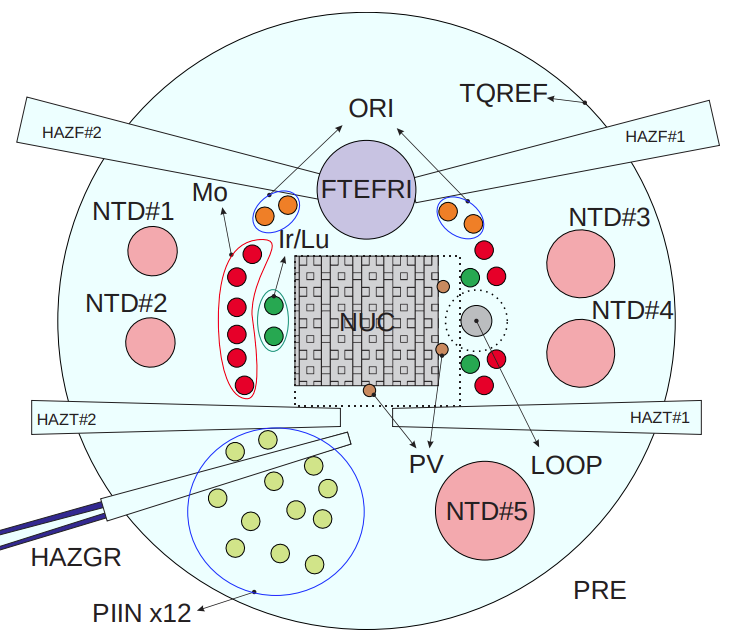
\includegraphics[width=0.95\textwidth]{figures/RA-10}
    \caption{Scientific research in the Argentinian reactor RA-10 \cite{ra10}.}
  \end{subfigure}
  \hfill
  \begin{subfigure}[b]{0.49\textwidth}
    \centering
    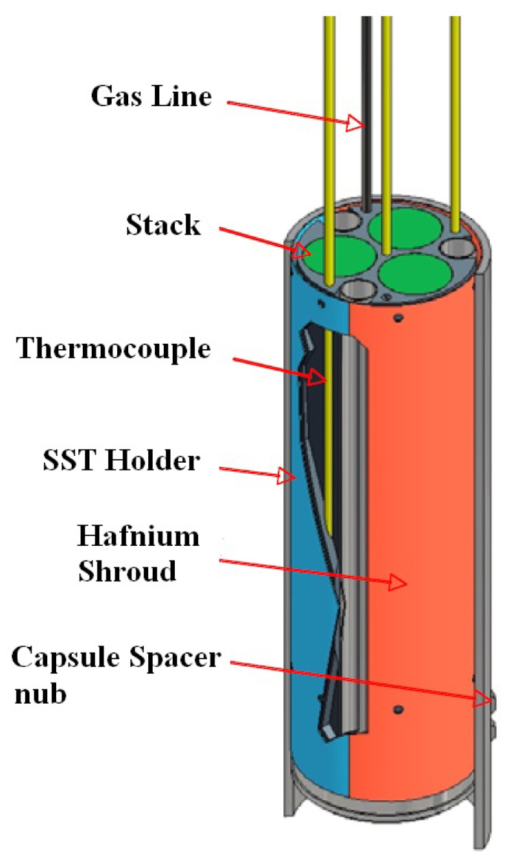
\includegraphics[width=0.50\textwidth]{figures/agr1}
    \caption{Material testing of the \gls*{AGR1} capsule \cite{sterbentz_agr1_2018}.}
  \end{subfigure}
  \hfill
  \caption{Examples of research reactor uses.}
  \label{fig:intro-1}
\end{figure}

% material testing
Material characterization and testing allows to study the effects of radiation on the material properties.
Neutrons induce changes in the materials' structure, making them fragile, elastic or hardened, swell, crumble, change their composition, release gas, etc.
Moreover, research reactors test advanced reactor fuel which supports their design optimization.
The \gls*{AGR1} experiment \cite{sterbentz_agr1_2018}, shown in Figure \ref{fig:intro-1}, was an irradiation test to provide performance data during normal operation of the fuel utilized in \glspl*{HTGR}.

% radioactive material production
Another frequent use of research reactors is radioactive material production, which encompasses three main applications: neutron activation analysis, neutron transmutation doping, and radioisotope production for medicine.
Figure \ref{fig:intro-2} shows some examples of these applications.
% neutron activation analysis
% https://www.iaea.org/sites/default/files/18/05/research-reactors-purpose-and-future.pdf
Neutron activation analysis is a technique to measure the elemental composition of water, air, soil, rocks, etc.
The samples are irradiated and by studying their characteristic gamma emissions it is possible to identify trace elements in the range of parts per billion.
% neutron transmutation
Neutron transmutation doping changes silicon properties, making it conductive, and the electronics industry highly benefits from this application for chip production.
% radioisotopes
Finally, the medical field utilizes radioisotopes for diagnosing and treating health conditions like cancer and cardiovascular diseases.
For example, technetium-99m comes from the decay of molybdenum-99, and its primary use is diagnostic imaging \cite{mattar_exploring_2019}.


\begin{figure}[htbp!] % or H
  \centering
  \begin{subfigure}[b]{0.45\textwidth}
    \centering
    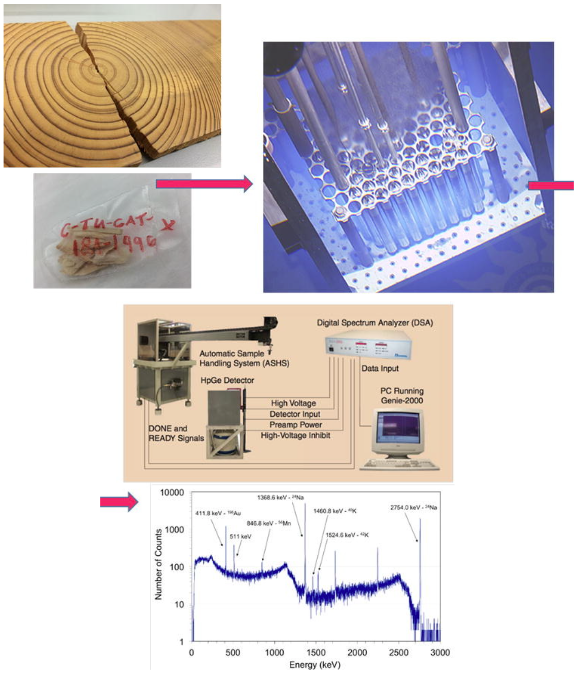
\includegraphics[width=0.75\textwidth]{figures/neutron-activation}
    \caption{Neutron activation analysis \cite{neutron-activation}.}
  \end{subfigure}
  \hfill
  \begin{subfigure}[b]{0.53\textwidth}
    \centering
    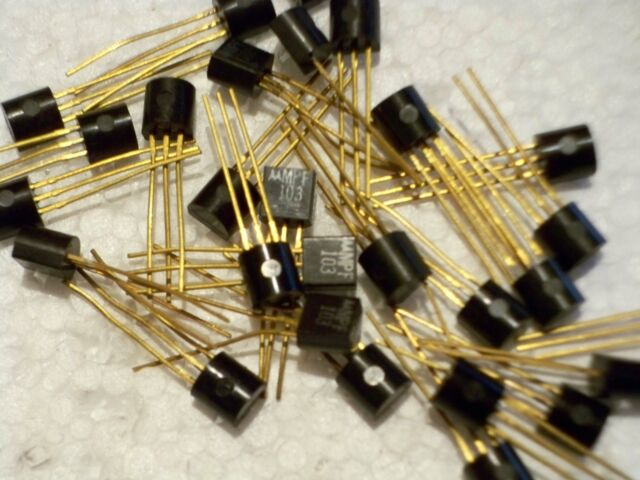
\includegraphics[width=0.95\textwidth]{figures/neutron-transmutation}
    \caption{Neutron transmutation doping.}
  \end{subfigure}
  \hfill
  \begin{subfigure}[b]{0.49\textwidth}
    \centering
    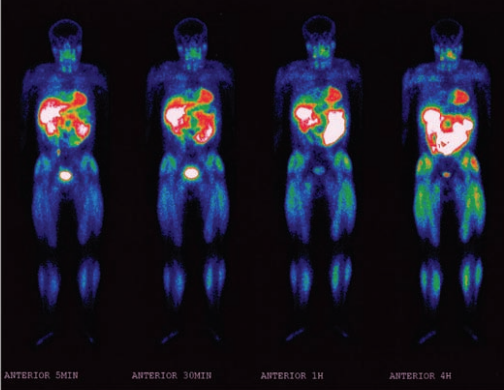
\includegraphics[width=0.95\textwidth]{figures/tc-99}
    \caption{Medicine applications. Whole body scan in a human administered with Tc-99m \cite{tc99m}.}
  \end{subfigure}
  \caption{Examples of applications of radioactive material production.}
  \label{fig:intro-2}
\end{figure}

% Some more: https://www.iaea.org/newscenter/news/exploring-research-reactors-and-their-use#:~:text=Research%20reactors%20are%20small%20nuclear%20reactors%20that%20are%20primarily%20used,and%20used%20to%20generate%20electricity.
% And some more: https://www.antinternational.com/docs/samples/FM/11/ZIRAT23_STR_Material_Test_Reactors_and_other_Irradiation_Facilities_Sample.pdf


\section{Motivation}

% https://www-pub.iaea.org/MTCD/Publications/PDF/Pub1321_web.pdf
% https://www-pub.iaea.org/MTCD/Publications/PDF/PUB1981_web.pdf

% Transition
The \gls*{IAEA} Safety Fundamentals state that the main safety objective in all nuclear installations is to protect people and the environment by establishing an effective defense against radiological hazards \cite{iaea-safety2}.
Fulfilling this objective requires the quantification of the risk of radiation release to the environment that may arise from a nuclear reactor.
Safety analyses assess the performance of the reactor against a broad range of operating conditions and demonstrate the prevention of radioactive material releases.
They can also identify hidden weaknesses and guide design improvements.
Although research reactors have a much smaller size and power than \glspl*{NPP}, safety analyses are still required.

Research reactor safety analyses demonstrate to the regulatory body the contribution of the operational procedures to the prevention and mitigation of accidents.
However, these analyses focus on the reactor core and disregard a thorough examination of the experiments.
This work defines an experiment as any device utilized in any of the aforementioned research reactor applications.
The development of experiment safety analyses is paramount to ensure safe experiment activities during any planned or unplanned events.
Accordingly, the \gls*{IAEA} recommends that experiment safety analyses include a list of possible hazards and any operational limits, such as maximum temperatures and pressures \cite{noauthor_safety_2012}.

% The problem
Research reactors enable the irradiation of a wide variety of experiments.
For example, they may have different combinations of shapes and materials.
Therefore, experiments tend to be unique, requiring independent calculations and the development of safety analyses on a case-by-case basis.
In consequence, the development of individual analyses often tends to be effort- and time-consuming.
% Also need for a unified workflow --> otherwise it is error prone
For instance, the initial experiment definition, design, and fabrication of a simple static capsule experiment for the \gls*{ATR} takes six months \cite{inl_advanced_2009}.
Nevertheless, using previously analyzed configurations can shorten this process.
%
Another example is the \gls*{NSUF} of the \gls*{HFIR}, wherein the experiment proposal review process requires the experiment materials and parameters to fall within the bounds of previously approved experiments \cite{hfir}.
For experiments falling outside these bounds, additional procedures are required, translating to longer processing times.
This reinforces the idea that using previous knowledge can expedite the process.

The present work supports the development of experiment safety analysis, and, to narrow down the scope of the analysis, it studies the bounding event - i.e., the most thermally challenging scenario that an experiment could undergo within the design basis accidents, a channel draining event.
The section on the left of Figure \ref{fig:diagra1} shows the standard workflow for the evaluation of the experiment state during the bounding event.
The workflow consists of a delayed heating calculation and the \gls*{CFD} modeling of the experiment.
The delayed heating calculation relies on a three-step process.
First, a neutron transport simulation determines the flux distribution.
Second, a depletion simulation determines the material composition, decay rates, and photon energy distribution.
Third, a photon transport simulation estimates the energy deposition in the experiment.
The subsequent run and exchange of information between these steps and the CFD simulation is commonly carried out manually by the lack of a streamlined workflow.
In consequence, the development of experiment safety analyses tends to not only be effort- and time-consuming, but also error-prone, as each of these steps introduces an instance for an error to occur.

\begin{figure}[htbp!]
  \centering
  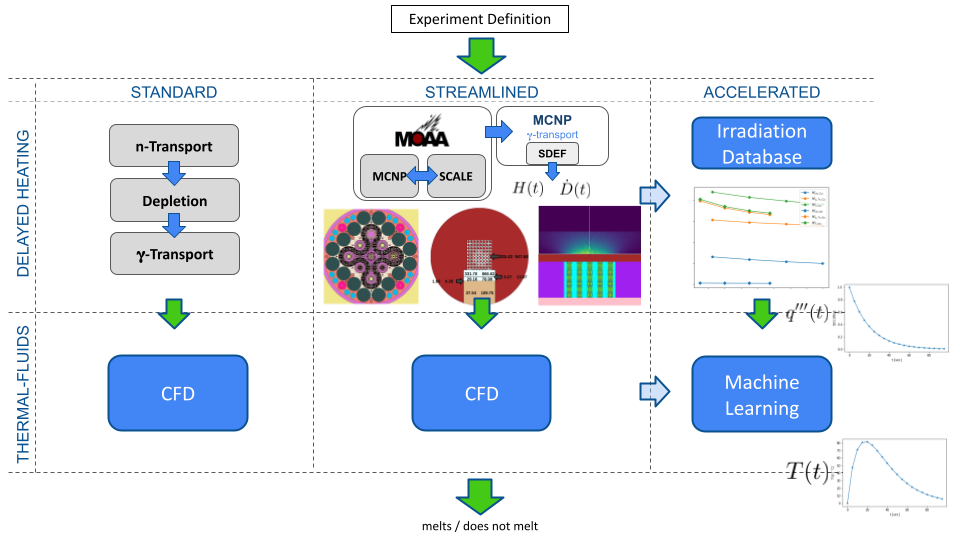
\includegraphics[width=0.99\textwidth]{figures/diagram}
  \caption{Calculation procedure to determine experiment state during a channel draining event.}
  \label{fig:diagra1}
\end{figure}


\section{Objectives}

% What is the main objective?
The objective of this Ph.D. thesis is to reduce the effort and time invested in the development of experiment safety analyses and to lower the chance of errors.
This objective can be separated into two parts.
The first part streamlines the calculation workflow, and the second part accelerates it by integrating previous knowledge into the process.
The section in the center of Figure \ref{fig:diagra1} provides a visual representation of the streamlined workflow that fulfills the requirements of the first part of the objective.
The streamlined workflow automates the transfer of information within the delayed heating calculation workflow as well as to the CFD simulation.
This objective can be organized into the following main subtopics.

% Secondary objectives
\textbf{Study the capsule's integrity during a channel draining event.}
Specifically, this work develops modeling capabilities to quickly predict the outcome of the bounding event on the experiment  and if it leads to a radioactive material release.
Additionally, the range of applicability of these capabilities should encompass any experiment material composition.
The present work considers the melting of the capsule encasing the experiment as the threshold for the radioactive material release.
The accident progression considers the following events: the safety system stops the fission reactions in the core, the experiment channel loses all the coolant, air fills up the remaining space, and the resulting natural circulation of air cools down the experiment.
The study takes a conservative approach and considers that the channel is drained instantly after shutdown.
% The following list of objectives expands on this goal.

% Thermal-fluids model
\textbf{Create a CFD model of the experiment.}
Effective heat removal prevents overheating damage that may lead to a radioactive material release.
Quantifying the capsule cooling requirements, and hence ensuring the capsule's integrity, requires the development of a thermal-fluids model to accurately predict the capsule temperature.

% Decay heat calculation
\textbf{Develop delayed heating calculation capabilities.}
In an operating reactor, there is an equilibrium between the generated and removed heat.
After a reactor shutdown, the radioactive materials continue to decay and release energy.
This energy is deposited across the reactor, and it is the cause of the delayed heating.
The assessment of the energy deposited in the experiment provides the thermal-fluids model with the volumetric heat source to accurately calculate the capsule temperature.
The delayed heating calculation workflow not only allows calculating the heating in the reactor experiments but also in reactor structures, a new feature that will be demonstrated.

% Shutdown dose rate calculation
\textbf{Shutdown-dose rate calculations.}
After the experiment has been extracted from the reactor, the ongoing decay exposes workers and equipment in the surroundings to radiation dose.
Safety analyses require the quantification of this dose.
A value-added of the delayed heating calculation is the shutdown-dose rate, which removes the need for additional workflow for radiation dose rates and will be demonstrated for the post-irradiation examination of an experiment.
% The calculation of the shutdown-dose rate will be demonstrated for the post-irradiation examination of AGR-1, a TRISO-fueled experiment in ATR.

The workflow described above streamlines the calculation procedure of experiment safety analyses.
The section on the right of Figure \ref{fig:diagra1} shows the accelerated workflow that intends to decrease the calculation burden significantly, which fulfills the requirement of the second part of this Ph.D. thesis objective.
The first part of the accelerated calculation is the delayed heating in the experiment, which relies on the use of the delayed heating calculation of the streamlined workflow.
This step entails the creation of a generic material irradiation database with which it is possible to estimate the delayed heating of experiments of any material composition.
The second component of the accelerated calculation is the determination of the bounding event outcome.
This part uses the CFD calculation of the streamlined workflow to train and test several machine-learning algorithms and examine their applicability to further lower the calculation burden.
This objective can be organized into the following main subtopics.

% Additionally, the proposed methodology includes the creation of a generic material irradiation database to further decrease the calculation burden.
% Furthermore, this work examines the applicability of machine-learning algorithms to reduce this burden even further.

\textbf{Generate a delayed heating database.}
Research reactors fulfill the radioisotope needs from multiple fields.
Consequently, the range of materials that form the experiments is vast.
For example, the medical field requires a supply of cobalt-60, yttrium-90, molybdenum-99, iodine-131, and iridium-192.
Therefore, this work aims to create a model extensible to all possible irradiated materials.
The creation of the database involves utilizing the delayed heating calculation scheme to obtain the delayed heating for experiments composed of individual chemical elements.
% Nevertheless, an experiment usually comprises a mix of different elements.
% This work creates a method for calculating the delayed heating of an experiment as a combination of the delayed heating of the individual elements that are part of it.
This work creates a method that uses such a database to calculate the delayed heating in experiments of arbitrary composition.
This method will be verified for selected materials.

% Surrogate model
\textbf{Build a data-based model.}
The thermal-fluids model allows for the determination of the capsule temperature for an experiment.
However, running the thermal-fluids model for each individual experiment is computationally expensive.
The data-based model utilizes several machine learning to further lower the computational burden and quickly predict the capsule temperature.
The present work compares their performance and examines their applicability to experiment safety analysis.
Ultimately, the data-based model aims to predict if the experiment capsule melts for any experiment material composition, provided its thermal properties are known.
Two main approaches were chosen.
The first approach relies on classification methods to predict the state of the experiment.
The second approach uses deep-learning to predict the temperature evolution of the experiment.

% Demonstrate in ATR
\textbf{Demonstrate the modeling capability by its application to ATR.}
The fulfillment of this thesis' objectives is complete with the application, demonstration, and verification of the presented developments on a full-size research reactor.
This thesis focuses on the \gls*{ATR}, and this objective consists of the following steps.
Create a detailed delayed heating database for an ATR experiment.
Tailor the thermal-fluids model to the experiment.
Train and test a data-based model specific to the experiment.


\section{Outline}

% TODO: I will get back to this after finishing the rest of the document
This thesis describes the motivation, objectives, methodology, results, and conclusions towards the advancement of the state-of-the-art of research reactor experiment analysis.
The remainder of this document is organized as follows.
Chapter 2 presents a literature review organizing and summarizing previous relevant work to this thesis.
Chapter 3 describes the delayed heating calculation workflow and demonstrates it for  multiple examples.
Chapter 4 focuses on the shutdown dose rate calculation workflow and several demonstration cases.
Chapter 5 introduces the generic material irradiation database method, and its verification with selected materials commonly used in nuclear engineering.
Chapter 6 describes the utilized machine learning algorithms, the implementation strategies, and the train and test of different exercises.
Chapter 7 summarizes the contributions of this thesis to the nuclear engineering field.

%%%% Figures
% \begin{figure}[htbp!]
% 	\centering
% 	\includegraphics[height=4.0cm]{figures/triso}
% 	\caption{Drawing of a TRISO fuel particle. Image reproduced from \cite{hales_multidimensional_2013}.}
% 	\label{fig:triso}
% \end{figure}

% \begin{figure}[htbp!]
%     \centering
%     \subfloat[Reactor layout. Image reproduced from \cite{barre_gas-cooled_2010}. \label{fig:fsv-a}]{
%         \includegraphics[width=0.40\textwidth]{figures/fsv-core}
%     }
%     \subfloat[Fuel assembly. Image reproduced from \cite{melese_thermal_1984}. \label{fig:fsv-b}]{
%         \includegraphics[width=0.41\textwidth]{figures/fsv-assembly}
%     }
%     \hfill
%     \caption{Fort St. Vrain Generating Station.}
%     \label{fig:fsv}
% \end{figure}


\chapter{Literature Review}
\label{ch:lit}

\section{Delayed Heating}

% Most of this comes from 8-/

% Research Reactor accident conditions - LOCA/LOFA : using the ANSI/ANS standard.
The state of the reactor core during an accident is the main focus of research reactor safety analyses.
Accordingly, numerous studies have targeted diverse accident conditions affecting research reactors, such as the \gls*{LOCA} and the \gls*{LOFA}.
% For example, Bajs et al. \cite{bajs_loca_2003} conducted numerical simulations of a LOCA in the IRIS Reactor.
Bajs et al. \cite{bajs_loca_2003} studied the performance of the emergency systems of the \gls* {IRIS} reactor during a LOCA concluding that the reactor core remains at safe temperatures and covered at all times during the event.
Kazeminejad et al. \cite{kazeminejad_thermal_2008} investigated the peak fuel and cladding temperatures of a 10-MW \gls*{IAEA} research reactor after a LOFA with flow inversion.
Hainoun et al. \cite{hainoun_international_2014} introduced a benchmark exercise for thermal-hydraulic solvers to study the LOFA in the IEA-R1 research reactor, where the metrics of interest were the coolant and cladding temperatures, reactor power, and flow rates of different positions in the core.
% And Abdelmaksoud et al. \cite{abdelmaksoud_analysis_2022} examined the passive heat removal by natural convection and radiation of a typical research reactor after a LOCA.
Abdelmaksoud et al. \cite{abdelmaksoud_analysis_2022} examined the possibility of passively cooling by natural convection and radiation the reactor core of a typical research reactor that is completely uncovered after a LOCA.
% % Other applications:
% Other studies targeted the design of nuclear facilities, such as spent fuel storage pools, spent fuel transportation systems, reprocessing plants, and final storage plants, to ensure their safeguards goal \cite{yamamoto_validation_2016}\cite{mozin_delayed_2011}.
% For example, dry storage facilities require the evaluation of the gamma radiation originating in the fuel \cite{gauld_applications_2006}.
% Localized heat deposition
All these studies rely on different versions of the ANSI/ANS standard \cite{ans_decay_1994} for estimating the decay heat after shutdown, assuming that most of the energy from radioactive decay is deposited locally in the region of interest: the reactor core.

Additionally, many software packages, such as Serpent \cite{giot_decay_2018} and ORIGEN \cite{scale}, estimate the decay heat by assuming the local deposition of heat, and diverse studies relied on the same assumption.
Lee et al. \cite{lee_decay_2010} used ORIGEN-2 to compare the decay heat in a \gls*{HTGR} core containing transuranic and uranium fuel.
Ilas et al. \cite{ilas_modeling_2015} calculated the decay heat in the HFIR irradiated fuel using ORIGEN-2.2.
% Some of their results revealed that their calculations yielded a decay heat 46\% larger than the ANSI/ANS standard.
% hawkes_sensitivity_2015 - I am not sure how the gamma heating is calculated, are gammas transported or just come from ORIGEN ? I think they just come from ORIGEN.
Hawkes et al. \cite{hawkes_sensitivity_2015} evaluated with ORIGEN-2.2 the thermal behavior of the AGR-2 experiment in the ATR, an experiment fueled with \gls*{TRISO} particles.
% The experiment heat rate was calculated with MCNP and JMOCUP \cite{sterbentz_mocup_2009}, featuring a couple utility program of MCNP5 and ORIGEN2.2.
% Need for precise method
However, an accurate assessment of the deposited energy across the reactor geometry can better determine the heat removal requirements and ensures an effective cool down.
Moreover, the regulatory authorities and the industry are interested in more precise calculations for economic reasons and \gls*{UQ}.
Therefore, instead of assuming the local deposition of heat, this work focuses on more detailed methods targeting the specific reactor regions hosting the experiments.

The main contributions to the nuclear heating in an operating reactor can be summarized as follows \cite{lemaire_estimation_2015}:
% Table \ref{tab:energy_fission} displays the different components of the energy released through fission.
% As this study places its focus on non-fueled regions of the reactor, the particles of interest are the ones that deposit their energy globally.
% These particles must be transported and heat is deposited during their trajectories.
% % Prompt (including capture gammas) and delayed gammas (from fission product decay) deposit their energy globally and must be transported as well.
% % Need to talk about the heat deposited by charged particles and the necessity of running a gamma-transport simulation.
% \begin{table}[htbp!]
%   \caption{Components of the energy released through fission \cite{brown_monte_2008}.}
%   \label{tab:energy_fission}
%   \begin{tabular}{llll}
%     Quantity                               & Notation        & Deposition site & Value(MeV)  \\
%     Kinetic energy of the fragments        &  Q$_f$          &  Local          & 169.12  \\
%     Kinetic energy of the prompt neutrons  &  Q$_{n,p}$      &  Global         & 4.79  \\
%     Kinetic energy of the delayed neutrons &  Q$_{n,d}$      &  Global         & 7.40E-03  \\
%     Kinetic energy of the prompt gammas    &  Q$_{\gamma,p}$ &  Global         & 6.97  \\
%     Kinetic energy of the delayed gammas   &  Q$_{\gamma,d}$ &  Global         & 6.33  \\
%     Total energy released by delayed betas &  Q$_{\beta}$    &  Local          & 6.50  \\
%     Energy carried away by the neutrinos   &  Q$_\nu$        & -               & 8.75  \\
%     Total energy release per fission (sum) &  Q              &                 & 202.47  \\
%     % Total energy less neutrino energy      &          &                 & 193.72
%     \end{tabular}
% \end{table}
\begin{itemize}
  \item Prompt neutron heating: deposition of the recoil energy of nuclei after a neutron collision and energy deposition of resulting charged particles from neutron interactions - e.g., heating caused by protons released in $(n,p)$ interactions.
  \item Delayed neutron heating: energy deposition of resulting charged particles created with a delay after a neutron interaction - e.g., heating caused by alpha particles resulting from actinide activation and heating caused by beta particles emitted from fission product decay.
  \item Prompt gamma heating: energy deposition of resulting charged particles of photo-atomic and photo-nuclear interactions. Prompt photons are emitted immediately after a neutron interaction. This includes prompt gamma radiation from the rapid de-excitation of the fission fragments and capture gammas.
  \item Delayed gamma heating: same energy deposition mechanism as prompt photons. Delayed photons are the result of activation and fission product decay.
\end{itemize}
% The delayed neutron contribution can be neglected as it is very low and decays within minutes.
% https://nuclear-power.com/wp-content/uploads/2015/10/Yield-of-Delayed-Neutrons.png
% U235 lambda_i [1/sec]: 1) 0.0124, 2) 0.0305, 3) 0.111, 4) 0.301, 5) 1.14, 6) 3.01
% T1/2_i [sec]: 1) 55.89 s ... it is the largest
% % I could include here the calculation of the prompt gammas
% % All contributions / prompt gamma contributions
% Several studies:
% - heating calculations including the prompt neutron, delayed neutron, and prompt gamma contributions
% - focus on determining the ratio between delayed and prompt gammas.
% % Prompt + delayed gamma
% Several studies \cite{lee_gamma_2001} \cite{amharrak_state_2014} \cite{fourmentel_delayed_2015} calculated the gamma heating during reactor operation, which includes both prompt and delayed components.
% % lee_gamma_2001: TRIPOLI-4 + DARWIN, only fission product decay-gammas
% % fourmentel_delayed_2015: TRIPOLI-4, only fission product decay-gammas ??
% % amharrak_state_2014: TRIPOLI-4 + PEPIN-2
% % ambrozic_JSIR2S_2020
% Ambrozic and Snoj \cite{ambrozic_JSIR2S_2020} compared JSIR2S calculations with experimental measurements to validate the code.
% % gruel_heating_2020
% Gruel et al. \cite{gruel_heating_2020} used JSIR2S to calculate the gamma field in the JSI TRIGA Reactor, including both prompt and delayed sources.
% JSIR2S is a code coupling MCNP and Fispact-II \cite{sublet_fispact_2017}.
% While MCNP is responsible for the transport of particles, Fispact-II handles the isotopic inventory and produces the source description for selected particles.
% Shutdown
After reactor shutdown, the prompt emissions no longer contribute to the heating, and we are left with only the delayed neutron and delayed gamma contributions.
% Local vs global
These contributions can be further classified by the location in which the emitted particles deposit their energy.
The delayed neutron heating is caused by charged particles that deposit their energy locally due to their short range.
The delayed gamma heating is caused by photons that deposit their energy globally and must be transported \cite{peterson-droogh_current_2018}.
The following formula calculates the nuclear heating after reactor shutdown or delayed heating
\begin{align}
H_{T} = H_{ch} + H_{\gamma, Tr} \label{eq:heat}
\end{align}
where $H_{T}$ is the total heat deposited in the region of interest, $H_{ch}$ is the energy deposited by charged particles in the region of interest, $H_{\gamma, Tr}$ is the energy deposited in the region of interest resulting from photon transport.

A common method for the calculation of the delayed gamma contribution is the so-called Rigorous 2-Step (R2S) process \cite{chen_rigorous_2002}.
Because the R2S process consists of three steps, this work refers to it as the \textit{formal 3-step process}.
This method consists of the following three steps:
\begin{itemize}
  \item First, a neutron-transport calculation determines the neutron flux spatial and energy distribution during reactor operation.
  \item Second, an activation calculation estimates the energy distribution and emission probability of the photon decay after reactor shutdown.
  \item Third, a photon-transport calculation evaluates the delayed gamma heating.
\end{itemize}

% Nuclear heating in experiment positions - Pre-defined values
Earlier versions of this method accounted for the delayed photons through a fixed-source calculation based on pre-defined gamma emission probabilities.
% ambrosek_improved_1995 - they also calculated the neutron and prompt photon heating
For example, Ambrosek et al. \cite{ambrosek_improved_1995} used this method to calculate the delayed gamma heating component in two ATR experiment positions.
% lee_tripoli_2013
Lee et al. \cite{lee_tripoli_2013} also used this method to calculate the gamma-radiation dose of multiple \gls*{PWR} spent fuel elements.

% Nuclear heating in experiment positions: formal 3-step process
% mozin_delayed_2011
% Mozin \cite{mozin_delayed_2011} implemented the formal 3-step process utilizing MCNP \cite{mcnp} and CINDER to assay the delayed gamma radiation of spent \gls*{LWR} fuel.
% Additionally, they investigated the delayed gamma spectra sensitivity to the actinide content of the fuel.
% Their method actually comprised of four steps, in which the processing of the gamma source was an independent step.
For the formal 3-step process, Mozin \cite{mozin_delayed_2011} utilized MCNP \cite{mcnp} and CINDER \cite{mcnp-cinder} to investigate the delayed gamma spectra sensitivity to the actinide content of spent \gls*{LWR} fuel.
% lemaire_estimation_2015
Lemaire et al. \cite{lemaire_estimation_2015} utilized TRIPOLI-4 \cite{tripoli4} and the point-depletion tool PEPIN-2 \cite{pepin2} to study the delayed gamma contribution from fission product decay in the Jules Horowitz Reactor.
% Lemaire et al. \cite{lemaire_estimation_2015} studied the nuclear heating from prompt neutron, prompt photon, and delayed photons in the Jules Horowitz Reactor.
% Their delayed photon calculation utilized TRIPOLI-4 \cite{tripoli4} and the point-depletion tool PEPIN-2 \cite{pepin2}.
% Their method only accounted for the delayed photons from fission product decay and not the activation product decay.
% noh_estimation_2018 - MCNP6 & ORIGEN-2.1
% Noh et al. \cite{noh_estimation_2018} studied the delayed gamma heating by radiation originated in the activated structures of the High flux Advanced Neutron Application ReactOr (HANARO), a 30-MW research reactor of the \gls*{KAERI}.
% Their implementation coupled MCNP6 and ORIGEN-2.1.
% They calculated the nuclear heating after approximately 8 years of reactor operation in an iridium sample located in multiple irradiation positions - i.e. inner core, outer core, and heavy water reflector tank.
% The calculations considered as radiation sources the structural materials near the irradiation capsule, including the fuel assembly flow tubes, the inner shell separating the reflector tank from the core, and the heavy water reflector tank.
Noh et al. \cite{noh_estimation_2018} coupled MCNP and ORIGEN to study the delayed gamma heating by radiation originated in the activated structures of the High flux Advanced Neutron Application ReactOr (HANARO), a 30-MW research reactor of the \gls*{KAERI}.
% peterson-droogh_current_2018
% Peterson-Droogh and Howard \cite{peterson-droogh_current_2018} summarized in a paper the modeling techniques for the production of iridium-192 in the \gls*{HFIR} at the \gls*{ORNL}.
% The paper described modeling techniques used for the calculation of the heating rates and the activity of the iridium targets.
% The calculation of these metrics are required by thermal-hydraulic calculations and post-irradiation handling.
% Additionally, detailed calculations help in the optimization process of the target design.
% They calculated the prompt neutron and gamma components as well as the delayed components.
% Their calculation scheme of the delayed components can be separated into two.
% The first method relied on the \textit{PIKMT} method, better detailed later in this chapter, for obtaining the delayed gamma contribution from fission product decay.
% The second method used the formal 3-step process for calculating the delayed gamma contribution from activation product decay.
% Their implementation utilized a coupling of MCNP and ORIGEN.
% They utilized ORIGEN, as well, for calculating the heat deposition of charged particles in the iridium targets.
% % The contribution of the prompt photons, delayed photons, and the charged particles from activation product decay are 54\%, 19\%, and 27\% of the total heating rate, respectively.
% % The contribution of the prompt and delayed neutron is negligible.
Peterson-Droogh and Howard \cite{peterson-droogh_current_2018} summarized the modeling techniques for the calculation of the heating rates and the activity of iridium-192 targets in the \gls*{HFIR} at the \gls*{ORNL}.
Their delayed heating calculation was separated into two methods.
The first method was the PIKMT method, described later in this chapter, for obtaining the delayed gamma contribution from fission product decay.
The second method calculated the delayed gamma contribution from activation product decay by coupling MCNP and ORIGEN.

% Other applications of the formal 3-step process
The dose rate evaluation of fusion reactor components is another common application of the formal 3-step process.
% chen_rigorous_2002
Chen et al. \cite{chen_rigorous_2002} calculated the shutdown dose rate of the \gls*{ITER} mid-plane maintenance port coupling MCNP and the FISPACT inventory code \cite{forrest_fispact_1998}.
Other studies using this method include \cite{serikov_advanced_2002, sauvan_development_2016}.
% sauvan_development_2016: R2SUNED = MCNP + ACAB

% Different methods: Direct 1-step process
Valenza et al. \cite{valenza_proposal_2001} introduced another method widely used for shutdown dose rate calculations in fusion reactors.
The method replaces the prompt gamma spectrum with a decay gamma spectrum, and it is better known as the Direct 1-step (D1S) method.
The method requires modifying the nuclear data library so that the delayed gamma radiation replaces the prompt gamma radiation.
For example, the delayed gamma rays from Co-60 replace the prompt gamma rays that accompany the Co-59 $(n, \gamma)$ reaction.
Additionally, the method relies on a depletion solver to account for the build-up and the decay of the considered radionuclides.
Other fusion reactor studies \cite{petrizzi_improvement_2001, palermo_shutdown_2017} used this same method.
% cited by noh_estimation_2008
For fission reactors, Lee et al. \cite{lee_analysis_2008} used this method to calculate the delayed gamma contribution in the HANARO reactor.
% Drawbacks
Although the D1S method is simple once the nuclear data is modified, it is most reliable when the generated radionuclides have short half-lives \cite{noh_estimation_2018}.

% Different methods: PIKMT method
The \textit{PIKMT} method has become predominant in the past few years for delayed gamma heating calculations.
It was first introduced by Brown et al. \cite{brown_monte_2008} and relies on the assumption that the prompt and delayed gamma spectra are similar.
The method uses one neutron-photon coupled simulation using the MCNP PIKMT card to evaluate the energy deposited by prompt gamma radiation originated at fuel fission events, and then it scales it to the delayed gamma component.
% brown_monte_2008
\begin{align}
H_{\gamma, d} &= Q_{\gamma, d} / Q_{\gamma, p} \times F6\!:\!p_{PIKMT}
\end{align}
where $H_{\gamma, d}$ is the delayed gamma heating from the fission product decay, $Q_{\gamma, p}$ and $Q_{\gamma, d}$ is the energy released from fission carried away by the prompt and delayed gamma components, and $F6\!:\!p_{PIKMT}$ is the MCNP $F6$ tally with the PIKMT card.

% PIKMT examples
% Ilas et al. \cite{ilas_impact_2013} used the PIKMT method for studying the conversion of the HFIR's core from \gls*{HEU} to \gls*{LEU}.
% The focus of the study was the neutronic poison buildup and heating rates in the reflector.
% The nuclear heating calculation consisted of two simulations: one for obtaining the neutron and prompt gamma components and the other for the delayed gamma component.
% They compared some of the results obtained with the PIKMT method against previous results obtained with the formal 3-step process for an HFIR reflector redesign study \cite{chang_high_1995}.
% The study concluded that the overall agreement between methods is excellent.
Ilas et al. \cite{ilas_impact_2013} used the PIKMT method for calculating the heating rates in the \gls*{HFIR}’s reflector during a \gls*{HEU} to \gls*{LEU} conversion study.
%
% Davidson et al. \cite{davidson_heat_2017} assessed the feasibility of converting HFIR's fuel from HEU to LEU as well.
% They utilized the PIKMT method for calculating the delayed gamma heating rates in different regions of the reactor.
Davidson et al. \cite{davidson_heat_2017} calculated the delayed gamma heating in different reactor regions using the PIKMT method for another HEU-to-LEU conversion study in HFIR.
% jurbandam_calculation_2018
Jurbandam \cite{jurbandam_calculation_2018} calculated the spatial heat distribution in the SAFARI-1 nuclear reactor, relying on the PIKMT method to account for the delayed gamma contributions.

% Different methods: conclusion
One of the main advantages of the PIKMT method over the formal 3-step process is that it requires only one coupled neutron/photon-transport simulation for obtaining the delayed gamma contribution.
However, it only accounts for the gamma radiation emitted from fission product decay.
In general, when the component of interest is located close to the fuel, the photons from fission product decay become the major contributor to the delayed heating \cite{lemaire_estimation_2015}.
% Actually lemaire says that the activation product contribution is smaller than 2%
In other cases, the photons from activation product decay may have higher contributions.
For those cases, only the formal 3-step process is applicable.
Additionally, the formal 3-step process obtains the charged particle contribution, which is a contribution neglected by the PIKMT method.
Furthermore, the PIKMT method obtains the delayed gamma contribution during reactor operation or immediately after shutdown.
Given that this work is concerned with the time evolution of the delayed heating, the only applicable method here is the formal 3-step process.

% \section{Safety analyis in Research reactors}
% Not sure where/if to place this
% The calculations refer to a document that I couldn't find
% Khericha and Pedersen \cite{khericha_experiment_2003} studied the integrity of an irradiated MOX capsule during a canal draining event.
% The study reveals that a minimum cooling time of 4 hours after reactor shutdown should be established for fueled experiments to assure that melting does not occur.


\section{Transport/Depletion Solvers Background}

% Most of this comes from 6-/

% Need to link the first section to this section
The first two steps in the formal 3-step process are accomplished by coupling a transport and a depletion solver.
This strategy determines the evolution of the material composition in the reactor during operation.
Depletion solvers ignore the geometry of the system, which underscores the need for a transport solver.
The transport solver generates geometry- and material-dependent parameters that the depletion solver relies on.
The depletion solver then calculates the material compositions and returns this information to the transport solver, and a cyclical transfer of information occurs, as shown in Figure \ref{fig:trans-dep}.
% After reactor shutdown, he material composition and the isotopes decay chain provide enough information to determine the energy distribution and emission probability of the photon decay.

\begin{figure}[htbp!]
  \begin{center}
    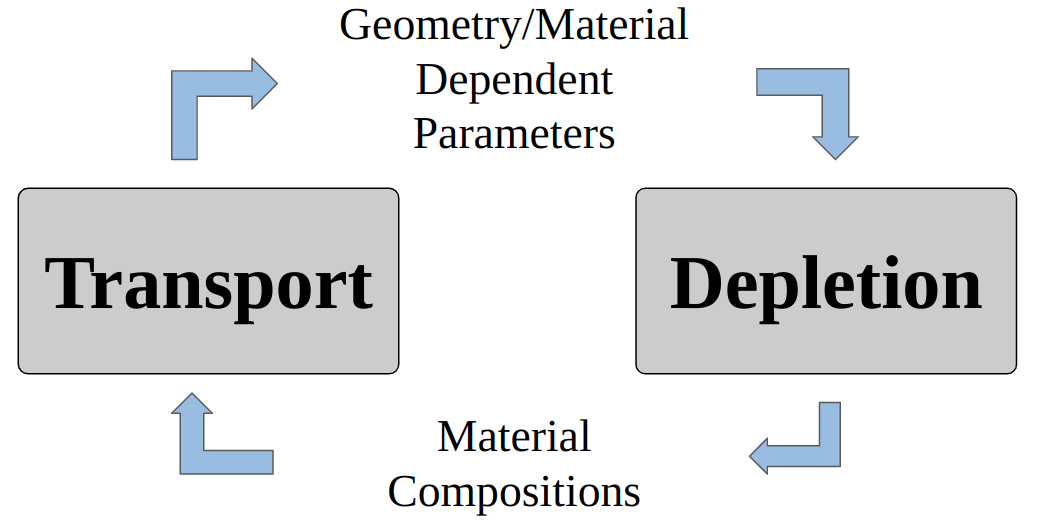
\includegraphics[scale=0.3]{figures/diagram_1}
  \end{center}
  \caption{Typical workflow of a transport/depletion solver.}
  \label{fig:trans-dep}
\end{figure}

There are several software packages available with these capabilities.
Table \ref{tab:background} summarizes some popular transport/depletion software packages that have been developed over the past 25 years.
This list is not meant to be extensive and instead provides the reader with an overview of past developments.
The motivation for the development of these tools varies.
Some were created to address specific projects, such as MOCUP \cite{mocup}, which was developed to simulate isotope depletion of the \gls*{ATR} and the Advanced Neutron Source, and Monteburns \cite{monte}, which was created to simulate isotope depletion for the Accelerator Transmutation of Waste (ATW) project at the \gls*{LANL}.

Additionally, MCNP’s lack of depletion capabilities motivated the development of many of these software packages, as well as the addition of depletion subroutines to MCNP itself \cite{mcnp-cinder}.
The integration of CINDER90 into MCNP provides a self-contained Monte Carlo/depletion capability in a single tool.
Serpent \cite{leppanen_serpent_2015} is another example of a Monte Carlo solver with self-contained depletion subroutines.

% MAYBE: add MCNP versions
\begin{table}[htbp!] %htbp! or H
  \centering
  \caption{List of previous Transport/Depletion software packages.}
  \label{tab:background}
  \begin{tabular}{ccccc}
    \toprule
    Tool       & Reference    & Transport  & Depletion  & Year developed \\
    \midrule
    MOCUP      & \cite{mocup} & MCNP       & ORIGEN2    & 1995 \\ %MCNP4A
    Monteburns & \cite{monte} & MCNP       & ORIGEN2    & 1998 \\ %MCNP4B
    MCODE-2.2  & \cite{mcode} & MCNP       & ORIGEN2    & 2008 \\ %MCNP4C
    VESTA      & \cite{vesta} & MCNP       & ORIGEN2/Phoenix & 2008 \\ %MCNP (any version)
    MCNP       & \cite{mcnp}  & \multicolumn{2}{c}{MCNP (CINDER90)} & 2009 \\ 
    Serpent    & \cite{leppanen_serpent_2015} & \multicolumn{2}{c}{Serpent (CRAM)} & 2010 \\
    \bottomrule
  \end{tabular}
\end{table}

Most of these tools, however, still rely on ORIGEN2, which was deprecated and lost support more than three decades ago.
The current version is ORIGEN/SCALE (sometimes called ORIGEN-S or just ORIGEN), which uses the \gls*{CRAM} \cite{cram} to solve the system of depletion equations.
While the open literature describes various depletion algorithms, the three most relevant are CINDER90 \cite{mcnp-cinder}, MATREX \cite{scale}, and \gls*{CRAM}.
MCNP uses CINDER90, ORIGEN2 uses MATREX, and ORIGEN uses either MATREX or CRAM.
The accuracy of the CINDER90 algorithm deteriorates for actinide prediction in higher-burnup cases \cite{mcnp-cinder}.
Although increasing CINDER90’s accuracy is possible by using a sub-step method, the CRAM solver produces more accurate solutions even when using longer burnup intervals \cite{vera}.
The MATREX algorithm is a hybrid method combining the Matrix Exponential method and linear chains \cite{origen2}.
While the matrix exponential and linear chains can be solved accurately when independent of each other, accounting for the effects of short and long-lived nuclides in the hybrid method requires additional approximations that lead to a loss of accuracy \cite{origen-cram}.
Overall, CRAM is orders of magnitude more accurate than other depletion algorithms currently available \cite{vera, origen2, origen-cram}.
Furthermore, in most cases, the solver is up to several times faster due to not having sub-stepping requirements \cite{origen-cram}.

% Motivation: ATR and active maintenance
As mentioned in Chapter \ref{ch:intro}, this work intends to demonstrate the modeling capabilities of ATR.
The physical configuration of ATR, shown in Figure \ref{fig:atr-view}, gives the reactor the unique capability to operate simultaneously at different power levels in the corner lobes.
This feature enables independent testing conditions within the same operating cycle for experiments located in different reactor regions \cite{atr}.

\begin{figure}[htbp!]  % or H
  \begin{center}
    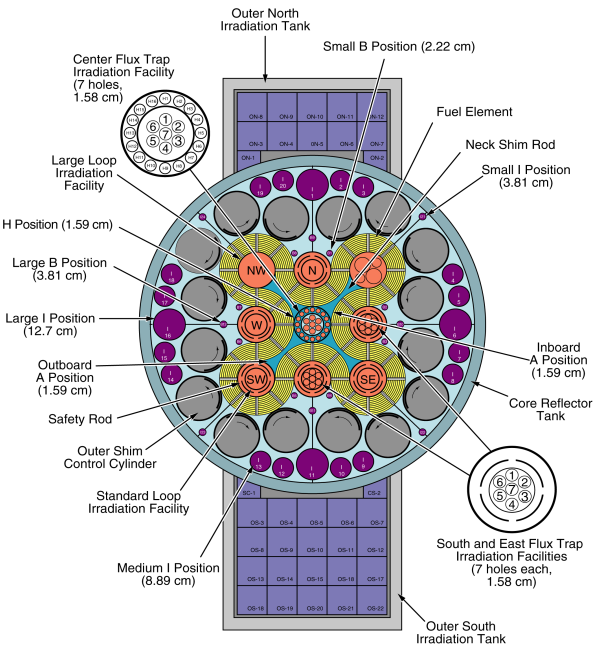
\includegraphics[scale=0.45]{figures/atr_view}
  \end{center}
  \caption{ATR cross sectional diagram and irradiation locations. Image reproduced from \cite{atr}.}
  \label{fig:atr-view}
\end{figure}

The analysis of ATR experiments requires the transport/depletion solver to have a lobe power scaling capability to properly calculate the neutron flux normalization factor and hence obtain the right depletion rates.
% A study within the section dedicated to MOAA could be to compare the flux and also depletion rates of an experiment when using and not using <atr>True</atr>.
While multiple tools have targeted ATR in the past, most of them are no longer maintained.
Active maintenance has many desirable features, including the development of new capabilities, bug catching and fixing, code updates for compliance with quality assurance requirements, among others.
% Motivation: computational requirments
% Finally, continuous energy Monte Carlo depletion calculations have high computational requirements, being memory-intensive tasks with long computation times \cite{vesta-2}.
Finally, continuous energy Monte Carlo depletion calculations have high computational requirements with long computation times.

% Conclusions
Overall, a tool relying on ORIGEN (and CRAM) that can model ATR and has low computational requirements can fulfill this thesis' needs.
The tool with all the desired capabilities is MOAA \cite{fairhurst_development_2022}, which is described in detail in Chapter \ref{ch:delayedheat}.


\section{Machine Learning}

% Why is this necessary?
As stated in Chapter \ref{ch:intro}, one of the objectives of this Ph.D. thesis is to accelerate the prediction of the bounding event outcome (capsule melts or does not melt).
This method relies on multiple machine learning algorithms.
This section of the thesis motivates the choice of the algorithms and describes them briefly.

% Intro
Machine learning is the branch of artificial intelligence that allows computer algorithms to derive relationships from data.
This feature allows them to solve complex problems, while at the same time decreasing the calculations' computational expense.
For example, the high computational expense of physics-based calculations makes them unsuitable for various applications, e.g., real-time reactor control.
Even though the \gls*{HPC} capabilities have increased considerably in the past few decades, they are still not sufficient.
In contrast, machine learning models can emulate the behavior of the input/output relationship of the physics-based model in real-time.

% Traditional ML
Traditional machine learning techniques have been applied in the nuclear engineering field to some extent.
% Safety analysis - Classification - SVM/SVR - IEEE Transactions of Nuclear Science
Na et al. \cite{na_detection_2008} applied \gls*{SVM} and \gls*{SVR} to \gls*{NPP} safety analysis.
During an accident, the NPP operators may have insufficient time to analyze the data and swiftly mitigate it.
Their work studied the applicability of \gls*{SVM} and \gls*{SVR} to a \gls*{LOCA} by predicting the break size and its location.
The model used multiple reactor signals, including core exit temperature, pressurizer water level, and containment pressure.

% Regression - SVR - Nuclear Engineering and Technology
NPPs safety systems calculate a number of safety-critical parameters and trip the reactor when they exceed the operating limits.
An accurate estimation of the local power density is necessary for the safe operation of an NPP for preventing the fuel rod from melting.
Bae et al. \cite{bae_estimation_2009} applied \gls*{SVR} to \gls*{NPP} online monitoring.
Their study accurately estimated the local power density based on different signals of the reactor coolant system, including reactor power, core inlet temperature, and coolant flow rate.

% Reactor control - Regression - SVR - Annals of Nuclear Energy
Zeng et al. \cite{zeng_machine_2017} created a machine learning-based system for autonomous control of small reactors.
The system consisted of a prediction module using \gls*{SVR} to estimate the state of some system variables, such as coolant and fuel temperatures, flux, and power history.
The prediction module fed into a decision module, which consisted of the control decision making and control system motion.
They demonstrated the system prediction module for a reactivity insertion event in a 20 MW$_{th}$ \gls*{TFHR}.

% Predictive maintenance - Classification - SVM and Logistic regression - Nuclear Engineering and Technology
Gohel et al. \cite{gohel_predictive_2020} developed a framework utilizing \gls*{SVM} and \gls*{LogR} for conducting predictive maintenance of \glspl*{NPP}.
Predictive maintenance allows operators to mitigate component failures and to increase the power plant availability.
Their framework intended to predict the failure of a power plant infrastructure in future cycles based on sensor real-time data.
Due to the lack of real NPP data, the paper demonstrated the framework by applying it to the degradation of a turbofan engine.

% Several - Nuclear Engineering and Design
Blevins and Yang \cite{blevins_machine_2020} discussed the suitability of machine learning for manufacturing in nuclear engineering.
Their article presented an overview and examples of applications of multiple machine learning techniques, such as \gls*{DTR}, \gls*{RFR}, \gls*{SVM}, \gls*{KNN}, and \glspl*{FNN}, to advanced manufacturing.
As many of these algorithms have not been yet applied to advanced manufacturing in the nuclear engineering field, they extrapolated these methods from different engineering applications, including semiconductor doping, manufacturing defect detection, and additive manufacturing parameter optimization, among others.

% Deep learning
Additionally, deep-learning, which is a sub-field of machine learning, has also been applied to nuclear engineering problems.
Deep-learning algorithms are more complex and abstract than traditional machine learning algorithms.
Nevertheless, a higher level of abstraction allows them to automate some pieces of the training process and, hence, eliminate some of the human intervention.
% Online Monitoring - ANNs - Nuclear Technology
In 1992, Guo and Uhrig \cite{guo_use_1992} presented one of the first applications of \glspl*{ANN} to nuclear engineering.
They developed a model for online monitoring that was able to predict the thermal performance and gross heat rate of the Sequoyah \gls*{NPP}.
The model utilized a hybrid neural network, comprising a clustering stage and an \gls*{FNN}, trained with sensor signals from the plant.
Additionally, they applied a sensitivity analysis to the network to determine the variables that affected the heat rate the most.
This kind of study allows power plant personnel to determine the cause of anomalies and, hence, provide a controlling basis for them.

% Optimization - ANNs - Annals of Nuclear of Nuclear Energy
Erdogan and Melih \cite{erdogan_pwr_2003} developed an optimal loading algorithm for nuclear fuel based on an \gls*{FNN} and a genetic algorithm.
Their algorithm searched for a loading pattern that minimized the initial amount of fuel and satisfied the reactor safety requirements.
Overall, minimizing the use of fuel reduces the operational cost of the plant.
% Optimization - ANNs - Annals of Nuclear Energy
% Fernandes-Faria and Pereira, 2003 \cite{fernandes-faria_nuclear_2003} utilized an \gls{ANN} for minimizing the power peaking factor while maximizing the fuel burnup.
% Control rod position - ANNs - Progress in Nuclear Energy
Andersson et al. \cite{andersson_development_2003} developed an application for online monitoring utilizing \gls*{FNN}.
The network calculated the control rod positions from the axial shape of the neutron flux.
Such an application helps to corroborate the control rod positions during transients.
The neural network could guide that control rod calibration process as well, as the electromechanical position indicators can be recalibrated during operation.
% Online Monitoring - ANNs - Annals of Nuclear Energy
% Souza and Moreira, 2006 \cite{souza_neural_2006} applied ANNs to reactor protection systems.
% Their paper intended to predict in real time the power peak factor based on the control rods position.
% Reactor design ? - ANNs - Annals of Nuclear Energy
Montes et al. \cite{montes_local_2009} applied FNNs to reactor fuel optimization.
The network quickly determined the local power peaking factor in a \gls*{BWR} based on the distribution of fissile and burnable poison materials.
The power peaking factor is a design parameter, and the ability to quickly estimate it reduces the fuel optimization time.
% Time evolution - ANNs - Nuclear Engineering and Design
Gomez Fernandez et al. \cite{gomez_fernandez_nuclear_2017} applied FNNs to reactor accident identification.
Their data comprised multiple sensor signals from a small \gls*{LWR} and the time evolution corresponding to two transient events, a piecewise-constant power ramp and a \gls*{LOFW} accident.
The model was able to accurately identify the transients and predict the time evolution of the reactor.
A model with such features can guide the \gls*{NPP} operators to identify safety issues and to take prompt actions to mitigate the accident.

% CNNs
Other examples of \glspl*{ANN} applied to nuclear engineering include the use of \glspl*{CNN} and \glspl*{RNN}.
For example, Kamuda et al. \cite{kamuda_comparison_2018} applied \glspl*{CNN} to automate isotope identification in gamma-ray spectroscopy.
Wilson \cite{wilson_machine_2019} compared the performance of \gls*{SVR} and a CNN at predicting the reactor power shape for diverse shim blade positions.
Their goal was to demonstrate that machine learning can provide real-time predictions and contribute to the autonomous control of nuclear reactors.

% RNNs
% https://www.analyticsvidhya.com/blog/2022/03/a-brief-overview-of-recurrent-neural-networks-rnn/
% LSTMs
% https://colah.github.io/posts/2015-08-Understanding-LSTMs/
% https://www.analyticsvidhya.com/blog/2021/03/introduction-to-long-short-term-memory-lstm/

% RNNs
\Glspl*{RNN} were created to handle inputs and outputs correlated as part of a sequence.
For example, when predicting the next word of a sentence, the prior words are necessary.
While all inputs and outputs in an FNN are independent of each other, an RNN is a sequential network that allows information to persist and uses it for processing the current input.
In the last few years, \glspl*{RNN} have been successfully applied to various tasks involving sequential inputs, such as speech and language recognition/prediction \cite{mikolov_recurrent_2010}.

% The problem - LSTM - Intro
In practice, RNNs cannot learn long-term dependencies.
When training the network, the back-propagated gradients may grow or shrink significantly at each time step.
Therefore, the gradients may vanish or explode for sufficiently long time series.
This issue is called the vanishing gradient problem, and \glspl*{LSTM} were explicitly designed to avoid it.
LSTMs are a special kind of RNN and are able to learn long-term dependencies.

% LSTM - yang_accident_2018
Yang and Kim \cite{yang_accident_2018} developed a model using LSTMs for accident diagnosis.
The model predicted the evolution of the plant's main variables and identified the accident.
% The trained model demonstrates the feasibility of utilizing LSTM for diagnosing several NPP accidents, including a loss of coolant accident, a steam generator tube rupture, and a main steam line break.
% LSTM - lee_autonomous_2018
Lee et al. \cite{lee_autonomous_2018} created a model using LSTMs for the autonomous operation of safety systems.
% Their model predicted the state of several plant components given multiple physical variables.
% % Given multiple physical variables the predicts the state of several plant components, and hence, reducing the role of human operators in critical decision making.
% % To train a validate their model, they used a compact nuclear simulator featuring a reference PWR.
% LSTM - radaideh_neural-based_2020
Radaideh et al. \cite{radaideh_neural-based_2020} predicted the progression of a \gls*{LOCA} utilizing deep-learning algorithms, including FNNs and LSTMs.
% They utilized two approaches: first, a \gls*{FNN} to fit all outputs in a single model, and second, a \gls{LSTM} network to fit individual models for each output.
% In this approach, the model makes one-step predictions, meaning that it uses the available data for the current time step \textit{t} to predict the following time step \textit{t+1}.
% Then, the actual data at \textit{t+1} is made available so it can be used for making a prediction on the subsequent time step.

% Other examples of LSTM usage outside the nuclear engineering domain include:
% - erosion rate and shoreline evolution forecasting for sandy coasts \cite{calkoen_traditional_2021}
% - speech recognition: Graves, A., & Jaitly, N. (2014). Towards end-to-end speech recognition with recurrent neural networks. International Conference on Machine Learning, 1764–1772.
% - language modeling: Kiros, Salakhutdinov, & Zemel, 2014

% Conclusion
Overall, machine learning has been applied to different areas of nuclear engineering.
The numerous applications described here cover many algorithms that can be classified as traditional machine learning or deep-learning.
This literature survey helps to understand the state of development of this field and can guide the choice of algorithms for this work.
% problem at hand.
However, machine learning has not been yet utilized in applications with similar objectives to this thesis'.
Therefore, Chapter \ref{ch:tf} compares various algorithms performance and analyzes their suitability to this thesis.


\chapter{Delayed Heating}
\label{ch:delayedheat}

\section{MOAA}

% PHYSOR - PRELIM
The Irradiation Experiment Neutronics Analysis group at the \gls*{INL} supports the \gls*{ATR} and the \gls*{TREAT} by performing neutronics analyses before the irradiation of experiments takes place.
% MAYBE - add more details to this ?
% Why is necessary to calculate the source term
The analyses provide the radioisotope source term of the experiments after irradiation.
% Can we cite previous work ?
The calculated source terms have multiple applications, which include radiation shielding, inventory and shipping purposes, demonstration of compliance with the safety limits, modeling of radioactive material dispersion, comparison to \gls*{PIE} results for validation, and experiment design and optimization, among others.

% Objectives
This section introduces the MCNP-ORIGEN Activation Automation (MOAA) tool and explains its workflow.
% why is MOAA necessary
The Irradiation Experiment Neutronics Analysis group developed MOAA to streamline the calculation of the experiment source terms.
% What is MOAA
MOAA is a Python package that couples MCNP \cite{mcnp} and ORIGEN \cite{scale} by writing MCNP tally cards, reading MCNP tallies, creating SCALE input files, executing SCALE, and standardizing the results post-processing.
Streamlining this procedure helps to reduce processing times and avoid potential human errors.

Although MOAA was originally developed to analyze the irradiation of experiments at ATR, it has grown to become a more general tool through further development.
Overall, MOAA is a tool that calculates radionuclide mass, activity, and heat in the regions of interest in a nuclear reactor.
% Other potential applications
% cite previous work and applications
Similar tools set a path for potential future applications for MOAA, including fuel burnup \cite{sterbentz_agr1_2018}, spent fuel repository design \cite{spent_fuel_2008}, transportation cask design \cite{transportation_2016}, shutdown dose calculation \cite{chen_rigorous_2002}, to mention just a few.
Additionally, earlier work utilized MOAA for delayed heating calculations \cite{fairhurst_decay_2022, fairhurst_demonstration_2022, fairhurst_database_2022}.
% See if there is any report that I could cite
% burnup of reactor with moving inventory \cite is there a report maybe?


\subsection{Calculation Workflow}

% Intro: single/multiple irradiations
MOAA performs material irradiation and decay calculations, which can be configured to include a single or multiple irradiation steps \cite{fairhurst_development_2022}.
While a single-step calculation uses constant power irradiation, multi-step calculations can handle several core configurations and piecewise constant power irradiation (i.e., different power levels at each time step).
Such capability allows for the modeling of evolution in material density, temperature, and geometry, as well as the control rod movement during the irradiation cycle.
% Predictor/Corrector
Additionally, the calculations can be configured to utilize the conventional predictor-corrector scheme, which is a two-step process that combines explicit and implicit calculations to achieve higher accuracy.

% General workflow - describe what each component does
% Figure \ref{fig:workflow_1} shows the calculation of the isotopic composition $m_l$ after irradiation case $l$.
% The subsequent irradiation case uses $m_l$ to update the MCNP material definitions.
\begin{figure}[htbp!]
  \begin{center}
    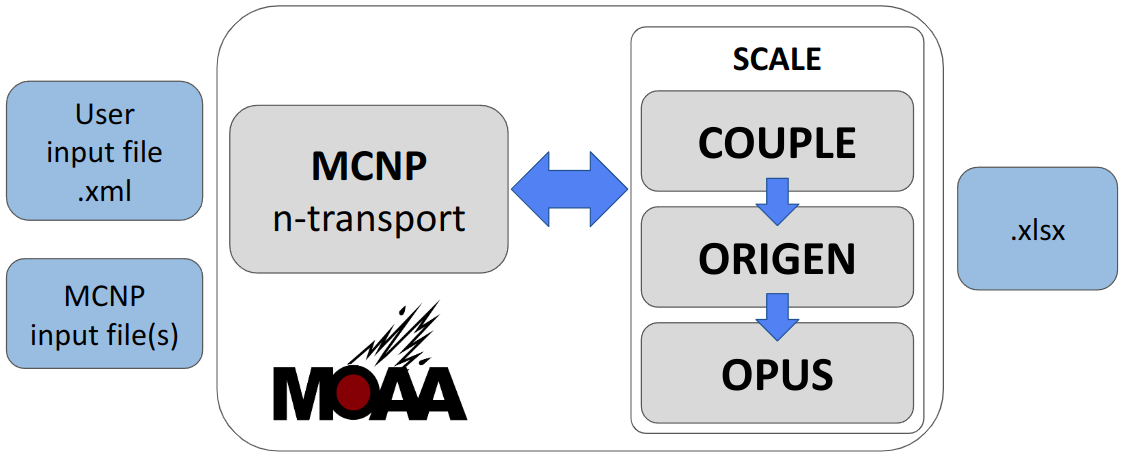
\includegraphics[scale=0.4]{figures/diagram_2}
  \end{center}
  \caption{Graphical representation of MOAA's workflow.}
  \label{fig:workflow_1}
\end{figure}

Figure \ref{fig:workflow_1} highlights MOAA's main calculation workflow that integrates with MCNP and ORIGEN.
MCNP is a general-purpose, continuous-energy, generalized-geometry, Monte Carlo radiation-transport tool that can track neutrons, photons, electrons, and other particles.
The main advantage of the Monte Carlo method is its capability to model geometry and interaction physics without significant approximations.
MOAA relies on MCNP for obtaining the geometry- and material-dependent parameters of the user-defined system during the irradiation steps - i.e., fluxes and reaction rates.

ORIGEN is a general-purpose point depletion and decay tool to calculate isotopic concentrations, radiation source terms, and decay heat.
ORIGEN is integrated into the SCALE code system, which is a modeling and simulation suite for nuclear safety analysis and design.
MOAA uses the calculated parameters from the MCNP output files to define the SCALE input files.
Besides ORIGEN, MOAA also uses the COUPLE and OPUS modules from SCALE.
ORIGEN requires a single volume- and spectrum-weighted cross-section library that MOAA generates using COUPLE.
Meanwhile, OPUS provides the ability to extract specific data from the ORIGEN output libraries, perform unit conversions, and generate data for post-calculation analysis.

% Formulas
MOAA calculates the following parameters for each cell of interest
% Need to double check the formulas
% isotopes: j
% reaction: k
% irradiation step: l
% predictor corrector: m = P or C
% irradiation case: l,m or n
\begin{align}
\phi(E)^{l, m} &= F4_{E} \\
\bar{\phi}_T^{l, m} &= \frac{\nu \times P [MW]}{Q [MeV/fiss] \times k_{eff} \times 1.6022 \times 10^{-19}} \times \mathlarger{\sum}_E F4_E \label{eq-flux} \\
\sigma_{j,k}^{l, m} &= \frac{ F4_{FM_{j,k}} }{ \mathlarger{\sum}_E F4_E } \\  % F4 tally_{FM}: the reaction cross-sections are microscropic (MCNP manual 3.3.5.7 Note 4)
k &= (n,\gamma), (n,p), (n,\alpha), (n,fission)
\end{align}
where $\phi(E)$ is the spectrum normalized to unity, $\bar{\phi}_T$ is the power-normalized total neutron flux, and $\sigma$ is the microscopic one-group cross-section.
The index $l$ corresponds to the irradiation step and index $m$ specifies the calculation to be the predictor or corrector case.
The index $j$ corresponds to the isotope identification number and index $k$ corresponds to the reaction type.
$F4_E$ is the F4 tally split up into energy bins, $F4_{FM_{j,k}}$ is the F4 tally for isotope $j$ reaction type $k$, $\nu$ is the number of neutrons emitted per fission, $P$ is the reactor power, $Q$ is the released energy per fission, and $k_{eff}$ is the effective multiplication factor.
MOAA extracts the parameters $\nu$, $k_{eff}$, $F4_E$, and $F4_{FM_{j,k}}$ from the MCNP output files, and $P$ and $Q$ are user-defined parameters.
A special use case is the ATR simulations in which $P$ has to be calculated.
Section \ref{sec:atr} gives further details on its calculation.

\begin{figure}[htbp!]
  \begin{center}
    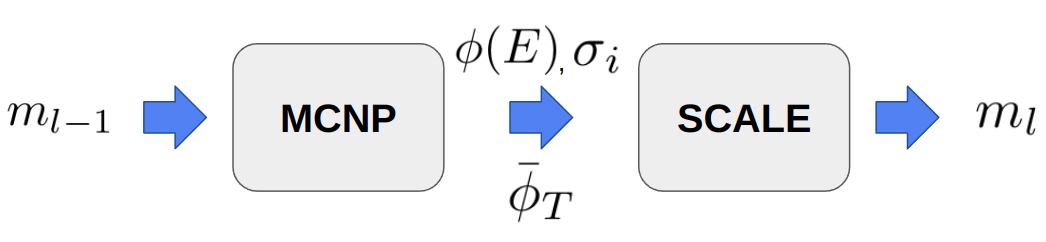
\includegraphics[scale=0.32]{figures/diagram_3}
  \end{center}
  \caption{Information flow of a MOAA simulation.}
  \label{fig:workflow_2}
\end{figure}

For multiple irradiation steps, MOAA calculates the isotopic composition at the end of the step $m_l$ based on the isotopic compositions from the previous step $m_{l-1}$, as shown in Figure \ref{fig:workflow_2}.
For the first irradiation step, the isotopic composition is extracted from the MCNP input file.
This method is known as constant extrapolation (CE) or Euler's method, which assumes that the flux and cross-sections remain at their beginning-of-step values throughout the interval \cite{leppanen_burnup_2012}.
If the predictor/corrector scheme is enabled, the irradiation step requires two irradiation calculations.
The first irradiation calculation uses $m_{l-1}$ to obtain $\phi(E)^{l, p}$, $\bar{\phi}_T^{l, p}$, and $\sigma_{j,k}^{p}$ to define the SCALE input files and calculate an intermediate isotopic composition $m_l^p$.
The second irradiation calculation uses $m_l^p$ to obtain $\phi(E)^{l, c}$, $\bar{\phi}_T^{l, c}$, and $\sigma_{j,k}^{c}$ and the following averaged parameters to define the SCALE input files and calculate $m_l$
% Predictor/Corrector formulas
\begin{align}
\phi(E) &= \frac{1}{2}\phi(E)^{l, p} + \frac{1}{2}\phi(E)^{l, c} \\
\bar{\phi}_T &= \frac{1}{2} \bar{\phi}_T^{l, p} + \frac{1}{2} \bar{\phi}_T^{l, c} \\
\sigma_{j,k} &= \frac{1}{2}\sigma_{j,k}^{l, p} + \frac{1}{2}\sigma_{j,k}^{l, c}.
\end{align}
This method is known as conventional predictor-corrector or constant extrapolation with linear interpolation (CE/LI) \cite{leppanen_burnup_2012}.
As the name suggests, the predictor calculation assumes constant values throughout the interval, and the final calculation uses an average of the predictor and corrector flux and cross-sections, which corresponds to a linear interpolation between the beginning and end-of-step values.

The creation of a MOAA application starts with the definition of a \gls*{UIF} in \textit{.xml} format, as shown in Figure \ref{fig:workflow_1}.
The UIF contains a set of required and optional settings for MOAA.
The required settings are a list of irradiation cases, a list of decay times, and a list of cells.
Within the irradiation cases, the user must specify an associated MCNP input file, an irradiation time, and an irradiation power.
% Basic user input description
Appendix \ref{ref:moaa-exec} displays a minimal MOAA input file.
MOAA's workflow can be summarized into Algorithm \ref{moaa_flow}.
If the predictor/corrector scheme is enabled, the number of cases is twice the number of irradiation cases.

\begin{algorithm}
  \caption{MOAA's main algorithm.}
  \label{moaa_flow}
  \begin{algorithmic}[1]
    \State parses user input file
    \For{case}
      \If {case $>$ 0}
        \State updates MCNP inputs with case-1 calculated compositions  
      \EndIf
      \State appends MCNP tallies
      \State executes MCNP
      \State parses MCNP output
      \If {case is corrector}
        \State applies correction
      \EndIf
      \State writes COUPLE sequence
      \State writes ORIGEN sequence
      \State writes OPUS sequence
      \State executes SCALE
      \State processes results
    \EndFor
  \end{algorithmic}
\end{algorithm}



\subsection{ATR cases}
\label{sec:atr}

The definition of an ATR case uses the same flux normalization as Equation \ref{eq-flux}, but requires the specification of the different lobe powers, as well as the calculation of adjusted lobe powers.
The adjusted lobe power can be thought of as a ``virtual'' total reactor power that would produce the same flux level in that lobe.
For experiments in lobes northwest (NW), northeast (NE), center (C), southwest (SW), and southeast (SE), the flux normalization uses the adjusted lobe power of the user-specified lobe powers.
The flux normalization of experiments in the rest of the lobes uses a weighted power average of the closest lobes.
For example, the east lobe (E) power is calculated as an average between the power of lobes NE, C, and SE.
The following formula calculates the adjusted lobe powers

% The tally number has to be user-specified with atr_lp_tally_id.
\begin{align}
T_i = \mathlarger{\sum}_c F7_{c} \times m_c \\
f_i = \frac{T_i}{ \mathlarger{\sum}_j T_j } \times \mathlarger{\sum}_j LP_j \\
P_i = \frac{LP_i}{f_i} \times \mathlarger{\sum}_j LP_j
\end{align}
where $F7_{c}$ is the fission energy tally, $m_c$ is the mass, and index $c$ represents the cells integrating the lobe.
$LP_i$ is the user-defined power for lobe $i$ and $P_i$ is the adjusted lobe power.
% ATR input file
The required settings within the irradiation cases include an MCNP input file, an irradiation time, an irradiation power divided into five lobe powers: NW, NE, C, SW, SE.
Additionally, the user must provide the F7 tally identification number that will be used for adjusting the lobe powers.
Appendix \ref{ref:moaa-exec} displays a typical UIF for an ATR irradiation experiment.


\subsection{Quality Assurance and Version Control}
\label{sec:quality}

% Quality Assurance
Nuclear regulators require the implementation of a quality assurance program for all systems that prevent or mitigate the consequences of postulated accidents in nuclear power plants and reprocessing plants.
Software plays a major role in licensing by producing calculations critical to the design and safety \cite{sqa}.
The implementation of a software quality assurance program ensures code reliability.

% NQA
This section briefly describes the current efforts for MOAA to fulfill the American Society of Mechanical Engineers (ASME) Nuclear Quality Assurance 1 (NQA-1) Standard \cite{nqa1}.
According to the NQA-1 documentation, ``this Standard reflects the current understanding of the quality assurance requirements necessary to achieve safe, reliable, and efficient utilization of nuclear energy, and management and processing of radioactive materials."
These requirements target different steps of the software development process, including \textit{software design requirements, software design, software implementation,} and \textit{software design verification}.
These steps entail the documentation of the entire process -- from the establishment of the software requirements to the confirmation that the design correctly fulfills them.
% 
The collection of these assets holistically qualifies MOAA for performing nuclear reactor physics analysis.
While this documentation discusses actions pertaining to the development of MOAA, MCNP and SCALE respective requirements are beyond the scope of this work.

% Releases
The NQA-1 standard requires reviews and approvals for each stable release, and a software test plan details the verification process that leads to such a release.
% Verification / Testing
The verification process comprises design reviews, alternative calculations, and/or testing.
Testing is the process of comparing the behavior of the observed code against its expected behavior.
The type of output for the different tests may range from numerical verification to error handling testing, covering behavior from the common to the extreme.
MOAA uses ``dynamic" testing, including white and black box techniques, to attempt to identify defects by executing the software.
All tests have the same objective, which is to ensure that the system produces the expected output when executed with the prescribed input.
This mechanism helps to provide confidence that the software performs as intended \cite{testing}.

% Directory tree
\begin{figure}[htbp!]
  \begin{center}
    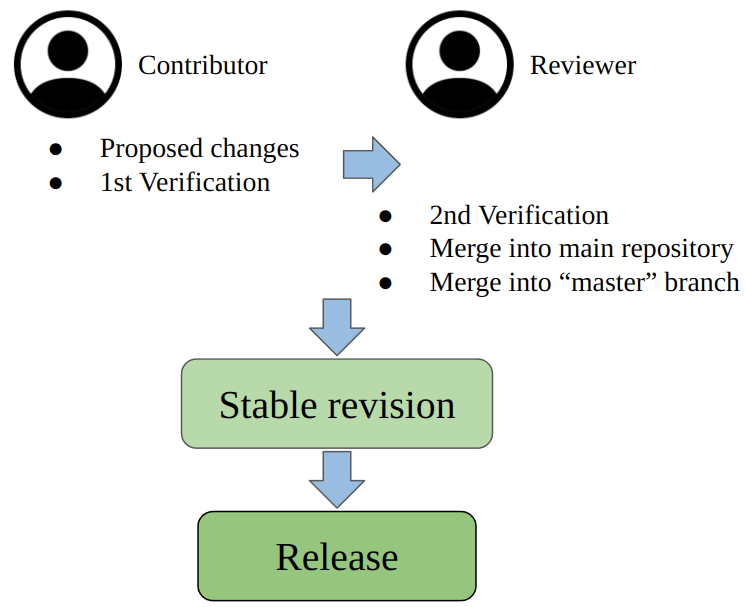
\includegraphics[scale=0.30]{figures/version-control}
  \end{center}
  \caption{Quality assurance process for MOAA.}
  \label{fig:sqa}
\end{figure}

% GitLab - Version Control
MOAA leverages the AGILE methodology for software development and tests that all proposed changes are properly integrated before merging them into the main repository hosting the source code, as shown in Figure \ref{fig:sqa}.
The proposed changes may include new features, which require the addition of new software design requirements, or a bug fix, which means that a software design requirement is not currently met.
After testing has been successfully completed (independently) by the contributor and a reviewer, a merge is made into the ``master" branch of the repository, creating a new ``stable" revision.
Each revision is eligible for release and subject to a complete release review.
Currently, a stable release of MOAA is under review.


\subsection{Simulation Specification}

To accommodate the MOAA calculations, the MCNP input files must undergo a few minimal modifications.
First, the depleted cells sharing the same material definition require the duplication of the original material, as each MOAA depleted cell requires an independent material definition.
The reason for this is to accommodate the depletion of independent cells subject to individual flux levels, divergent depletion rates, and the resulting different material compositions.

Second, while MOAA can handle the depletion of cells defined as repeated structures, it cannot handle the depletion when the same cell is present in different nested structures.
For example, if cell 100 is nested in cells 300 and 900 (100 $<$ 300 $<$ 900), and cell 100 is also nested in cells 400 and 900 (100 $<$ 400 $<$ 900), MOAA can handle only one of the two nested structures in one given simulation.
To handle both nested structures, cell 400 would have to be redefined as 300 if the geometry definition allows, and MOAA will be able to handle both occurrences simultaneously.

Third, the volume of some depleted cells has to be calculated and specified within the MCNP input file.
This is because MCNP can only calculate the volume of simple geometries only, and the user must specify the cell volumes to avoid errors.
For cells defined as repeated structures, the user must specify the volume of the whole material in those cells that is present in the geometry.
Otherwise, MCNP will calculate the volume of only one cell.


% Results
% Depletion results: AGR1 benchmark
\section{Delayed heating}

% This is probably repeated somewhere
In an operating reactor, an equilibrium exists between the generation and removal of heat.
After reactor shutdown, radioactive decay continues to release energy, which is deposited across the reactor and causes the delayed heating.
The estimation of delayed heating in experiments and in the reactor structures is paramount in the safety analyses of research reactors, and its accurate determination generates a reliable heat source term for thermal-hydraulics calculations.
This in turn allows the determination of heat removal requirements and evaluation of temperature levels in the components of interest \cite{fairhurst_decay_2022, fairhurst_machine_2022, fairhurst_machine_2_2022}.
Additionally, detailed calculations help in the optimization process of the irradiation target designs \cite{peterson-droogh_current_2018}.

Overall, these calculations determine whether delayed heating presents a hazard for the components of interest, which could lead to the release of radioactive contaminants into the reactor coolant.
An important application example is in spent nuclear fuel where delayed heating calculations are crucial for the design of nuclear facilities, including spent fuel storage pools, spent fuel transportation systems, reprocessing plants, and final storage sites.

% Objectives of the paper
This section introduces a delayed heating calculation workflow based on MOAA, presents the motivation for the choice of the method, and showcases its capabilities by presenting two specific applications.

\subsection{Calculation Workflow}
\label{sec:delheat}

Figure \ref{fig:workflow_0} summarizes the calculation workflow, which relies on the formal 3-step method for the delayed heating calculation.
During reactor operation, the first two steps in the formal 3-step process are accomplished by coupling a transport and a depletion solver.
The delayed heating calculation workflow presented here relies on the \gls*{MOAA} tool \cite{fairhurst_development_2022} for carrying out the first two steps.
After reactor shutdown, the depletion solver calculates the energy distribution and emission probability of the photon sources.
The photon-transport calculation uses this information to evaluate the delayed gamma heating.

%% General workflow
\begin{figure}[htbp!]
  \begin{center}
    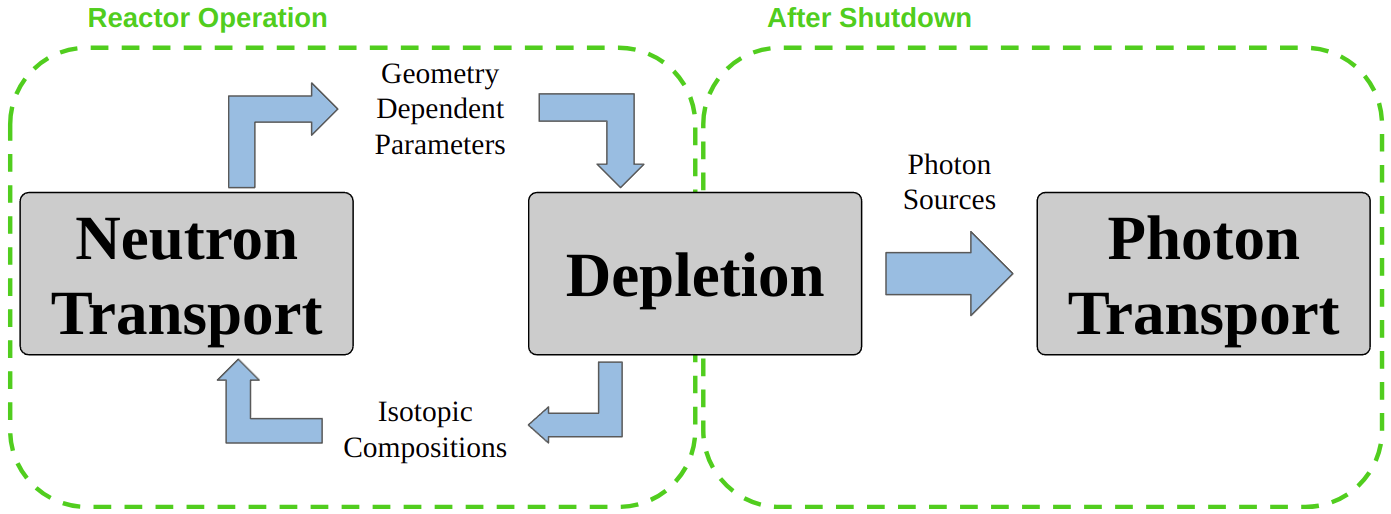
\includegraphics[width=0.80\linewidth]{figures/calc_w}
  \end{center}
  \caption{Calculation workflow diagram.}
  \label{fig:workflow_0}
\end{figure}

The delayed heating calculation can be separated into two parts.
The first part calculates the deposition of energy from charged particles $H_{ch}$.
This part includes only the charged particles that originated in the geometry of the component of interest and assumes that all the particles with mass deposit their energy in the region of interest.
The following equations calculate $H_{ch}$ \cite{giot_decay_2018, endf, peterson-droogh_current_2018}:

\begin{align}
H_{T, L} &= \mathlarger{\sum}_j N_j \lambda_j \bar{E}_j \\
H_{\gamma, L} &= \mathlarger{\sum}_j N_j \lambda_j \bar{E}_{EM, j} \\
\bar{E} &= \bar{E}_{EM} + \bar{E}_{HP} + \bar{E}_{LP} \\
\bar{E}_{EM} &= \bar{E}_{\gamma} + \bar{E}_{X-ray} + \bar{E}_{annih.rad.} + ... \\
\bar{E}_{HP} &= \bar{E}_{\alpha} + \bar{E}_{SF} + \bar{E}_{p} + ... \\
\bar{E}_{LP} &= \bar{E}_{\beta^-} + \bar{E}_{\beta^+} + \bar{E}_{Ae^-} + ... \\
H_{ch} [W] &= H_{T, L} - H_{\gamma, L}
\end{align}
where $H_{T, L}$ is the total decay heat, $N_j$ is the number of nuclei $j$, $\lambda_j$ is the decay constant of nucleus $j$, $\bar{E}_j$ is the total energy available (excluding neutrino energies) per decay of nucleus $j$, $H_{\gamma, L}$ is the total gamma heating, $\bar{E}_{EM}$ is the electromagnetic component, $\bar{E}_{HP}$ is the heavy particle component, $\bar{E}_{LP}$ is the light particle component, $\bar{E}_{\gamma}$ is the average gamma-ray energy, $\bar{E}_{x-ray}$ is the average X-ray energy, $\bar{E}_{annih.rad.}$ is the average annihilation energy, $\bar{E}_{\alpha}$ is the average $\alpha$ energy, $\bar{E}_{SF}$ is the average spontaneous fission energy, $\bar{E}_{p}$ is the average proton energy, $\bar{E}_{\beta^-}$ is the average $\beta^-$ energy, $\bar{E}_{\beta^+}$ is the average $\beta^+$ energy, and $\bar{E}_{Ae^-}$ is the average Auger-electron energy.

The second part calculates the deposition of energy from photons $H_{\gamma, Tr}$.
Because photons deposit their energy globally, photon transport is required, and this includes the photons originating from across the reactor.
The following equations describe the delayed heating
\begin{align}
H_{T} [W] &= H_{ch} + H_{\gamma, Tr}  \label{eq-heat} \\
H_{\gamma, Tr} [W] &= 1.6022 \times 10^{-13} \times \: ^* \! F8 [MeV] \times \mathlarger{\sum}_i S_i \label{eq-ga-tr} \\
S_i[\gamma/s] &= \int_{E} \varphi^\gamma_i(E) dE \\
s_i [-] &= S_i / \mathlarger{\sum}_j S_j \label{eq-emiprob}
\end{align}
where $H_{T}$ is the total heat deposited in the region of interest, $H_{ch}$ is the energy deposited in the region of interest by charged particles, $H_{\gamma, Tr}$ is the energy deposited in the region of interest resulting from the photon transport, $^\ast F8$ is the energy deposition calculated by an $^\ast$F8 tally, $S_i$ is the total photon emission rate from the region $i$, $\varphi^\gamma_i(E)$ the photon source energy distribution from region $i$, and $s_i$ is the source cell emission probability.

Overall, the calculation scheme follows the formal 3-step process, in which MOAA conducts the first two steps, and multiple MCNP photon-transport simulations conduct the third step, calculating the delayed gamma heating.
Figure \ref{fig:workflow_3} shows the calculation workflow.
MOAA calculates $H_{T,L}$ and $H_{\gamma, L}$ in the component of interest assuming those to be locally deposited.

\begin{figure}[htbp!]
  \begin{center}
    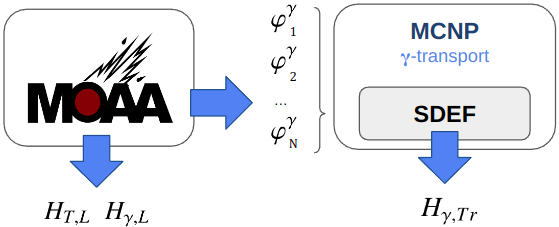
\includegraphics[width=0.70\linewidth]{figures/heat-flow}
  \end{center}
  \caption{Delayed heating calculation scheme relying on MOAA.}
  \label{fig:workflow_3}
\end{figure}

MOAA calculates $\varphi^\gamma_i(E)$ for all the cells defined by the user as contributors to the delayed heating.
The MCNP photon-transport simulations require the definition of a fixed source for these cells.
The source energy distribution is specified with $\varphi^\gamma_i(E)$.

The photon-transport calculation can be performed with multiple simulations, in which one simulation obtains the heat contribution for one source cell, or with one simulation, in which the simulation obtains the heat contribution for all the source cells simultaneously.
While the former determines the individual contributions from the different cells, the latter is computationally less expensive.
Nonetheless, the latter requires the definition of the cell emission probabilities $s_i$ using Equation \ref{eq-emiprob}.

The source spatial distribution is assumed uniform in each source cell.
For uniformly sampling the birth of a particle in a cell, MCNP uses the enclosing volume rejection method, which requires the user definition of a volume enveloping the source cell.
The randomly sampled points in the volume are accepted as source points only if they fall inside the source cell.
Finally, the photon transport estimates $^\ast F8$, which allows the calculation of $H_{\gamma, Tr}$ (Eq. \ref{eq-ga-tr}).


\subsection{Simulation Specification}

The calculation workflow requires the MOAA UIF and at least one MCNP input file defining the problem geometry.
However, the user may want to use different geometries for the neutron and photon transport and both MCNP input files should be defined.
This feature gives the calculation workflow great flexibility, allowing the user to model more complex scenarios.
For example, a study case can be the delayed heating sensitivity to long burnup in a reactor where there is fuel assembly shuffling.
Additionally, Chapter \ref{ch:sdr} studies cases where nuclear fuel is burned in the core, but the focus of the study is the shutdown dose rate for the \gls*{PIE}.

The delayed heating calculation requires two additional scripts: \texttt{run\_case.py} and \texttt{source\_gen.py}.
The script \texttt{run\_case.py} is the main workflow driver, and its role is summarized into Algorithm \ref{dh_flow}.

\begin{algorithm}
  \caption{Delayed heating main algorithm.}
  \label{dh_flow}
  \begin{algorithmic}[1]
    \State initializes delayed heating object
    \State reads source information
    \State creates neutron transport input files
    \State runs MOAA
    \State assigns lattice numbers to cells in repeated structures
    \State processes photon sources
    \State divides sources into batches
    \State creates photon transport input files
    \State runs MCNP for photon transport
    \State processes results
  \end{algorithmic}
\end{algorithm}

The script \texttt{source\_gen.py} allows for the automation of the photon source geometry definition.
This script defines the dimensions of the source where the particle birth is randomly sampled.
In the workflow described here, the user can define either a parallelepiped or a cylinder as the source geometry.
Appendix \ref{ap:mcnp_fixed} provides further details on the use of the delayed heating calculation workflow.


% Delayed Heating Results
\section{Results}
\label{sec:results}

This section presents and discusses the results of four exercises.
The first exercise is a code-to-code comparison between the workflow presented here and the Serpent Monte Carlo tool \cite{leppanen_serpent_2015}.
The second exercise demonstrates the calculation workflow for a simple case geometry.
The third exercise consists of the delayed heating calculation of an ATR experiment.
Finally, the fourth exercise analyzes the delayed heating in various structures in the RA-6 reactor.


\subsection{Delayed Gamma in a Uranium Sphere}

% Intro
This exercise studies the delayed gamma heating in a sphere of uranium.
The purpose of this study is to understand the foundation of the method by comparing the results with Serpent.
The Serpent Monte Carlo tool is a three-dimensional continuous-energy neutron transport application developed by the VTT Technical Research Centre of Finland, and it has been in public distribution since 2009.
This work uses Serpent 2.1.32 and the cross-section library ENDF/B-VII.0 for the calculations.
The choice of nuclear data was based on their availability.
This work uses Serpent because of its built-in burnup calculation routine.
Moreover, Serpent is capable of calculating delayed gamma heating in a two-step process.
The first step consists of a transport/depletion calculation that saves the radioactive material composition in a binary restart file.
The second step is a photon-transport simulation that generates the photon source based on the binary restart file.
This second simulation creates a \textit{\_gsrc.m} file specifying the gamma source distribution (see Appendix \ref{ap:serpent_gsrc} for further details).

The problem geometry includes a sphere of uranium surrounded by water, and it is shown in Figure \ref{fig:exp}.
The study focuses on the last component of equation \ref{eq-heat}, the heat generated by the transported gamma radiation $H_{\gamma, Tr}$.
% Describe model
The gamma heating is calculated after a 50 day-burnup at a constant power of 5 MW.

\begin{figure}[htbp!]
  \begin{center}
    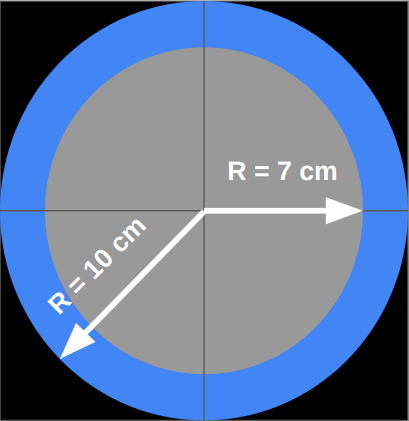
\includegraphics[width=0.35\textwidth]{figures/axial-view2}
  \end{center}
  \caption{Geometry of a sphere of uranium surrounded by water.}
  \label{fig:exp}
\end{figure}

% Results
The exercise compares the results of the nuclear heating calculation scheme developed here and Serpent.
Serpent provides the reference values for calculating the relative difference employing the following equation.
\begin{equation}
\textrm{Rel. Difference } [\%] = \frac{R_{\textrm{Serpent}} - R_{\textrm{MOAA}}}{R_{\textrm{Serpent}}} \times 100
\label{eq-rel-diff}
\end{equation}
where $R$ is the result of interest, which can be the integral flux, the mass of a nuclide, or gamma source intensity.

Table \ref{tab:gam-heat-results} summarizes the main results for different stages of the calculation.
The first stage is the burnup calculation.
The relative difference for the total neutron flux before burnup is below 1\%.
After burnup, the relative difference for the masses of U-235 and U-238 is below 1\% as well.

% Table
\begin{table}[htbp!]
  \centering
  \caption{Summary of the main results of the delayed heating calculation. $^1$ Before burnup. $^2$ After burnup.}
  \label{tab:gam-heat-results}
  \begin{tabular}{ccccc}
  % \begin{tabularx}{\textwidth}{ @{} L C{0.4} C{0.4} C{0.4} @{}}
    \toprule
                                & Units                     & MOAA/ MCNP & Serpent & Rel. Diff. [\%] \\
    \midrule
    $^1$Tot. neutron flux       & $10^{-3}/cm^{-2}/source$  & 3.9376  & 3.9284  & 0.24    \\
    $^2$U-235 mass              & $kg$                      & 25.279  & 25.279  & 0.01    \\
    $^2$U-238 mass              & $kg$                      & 2.835   & 2.835   & 0.01    \\
    $^2$Photon source intensity & $10^{17}\gamma/s$         & 10.16   & 4.65    & 118.40  \\
    $^2$Tot. gamma flux         & $10^{14}/cm^{-2}/s$       & 2.6464  & 1.7805  & 48.63   \\
    $^2$H$_{\gamma, Tr}$        & $kW$                      & 73.969  & 48.037  & 53.98   \\
    $^2$H$_{\gamma, Tr}/source$ & $10^{-14} \cdot J/source$ & 7.283   & 10.332  & -29.51  \\
    \bottomrule
  \end{tabular}
\end{table}

Figure \ref{fig:g-source} displays the gamma source distribution from radioactive decay after burnup.
MOAA uses 101 groups to obtain the source energy distribution and Serpent's data are formulated in the form of discrete lines.
There are some clear discrepancies around 10 keV between Serpent and MOAA caused by the Bremsstrahlung radiation.
While ORIGEN accounts for the photons originated by the deceleration of charged particles, Serpent considers only the photons originated directly from radioactive decays.
In opposition, the upper range of the source distribution shows better agreement.

MOAA predicts a photon source intensity more than two times greater than Serpent, as shown in Table \ref{tab:gam-heat-results}.
The origin of this discrepancy is mainly attributed to the consideration of the Bremsstrahlung radiation into the calculations.
Additionally, understanding the discrepancies requires some grasp of the algorithms in MOAA and Serpent.
In MOAA, COUPLE provides ORIGEN with the cross-section library necessary for the depletion calculation.
COUPLE creates by default spectrum-averaged cross-sections based on JEFF-3.0/A and replaces them with the cross-sections generated from the MCNP neutron transport calculation.
The cross-section values that are not replaced still use the JEFF spectrum-averaged cross-sections.
Monte Carlo solvers, such as MCNP and Serpent, track all necessary reaction rates and follow all the isotopes available in the nuclear data.
While MOAA relies primarily on ENDF/B-VII.1, it still depends on JEFF-3.0/A.
Consequently, MOAA and Serpent predict different after-burnup compositions, which translate into different photon source intensities.

\begin{figure}[htbp!] %or H 
    \centering
    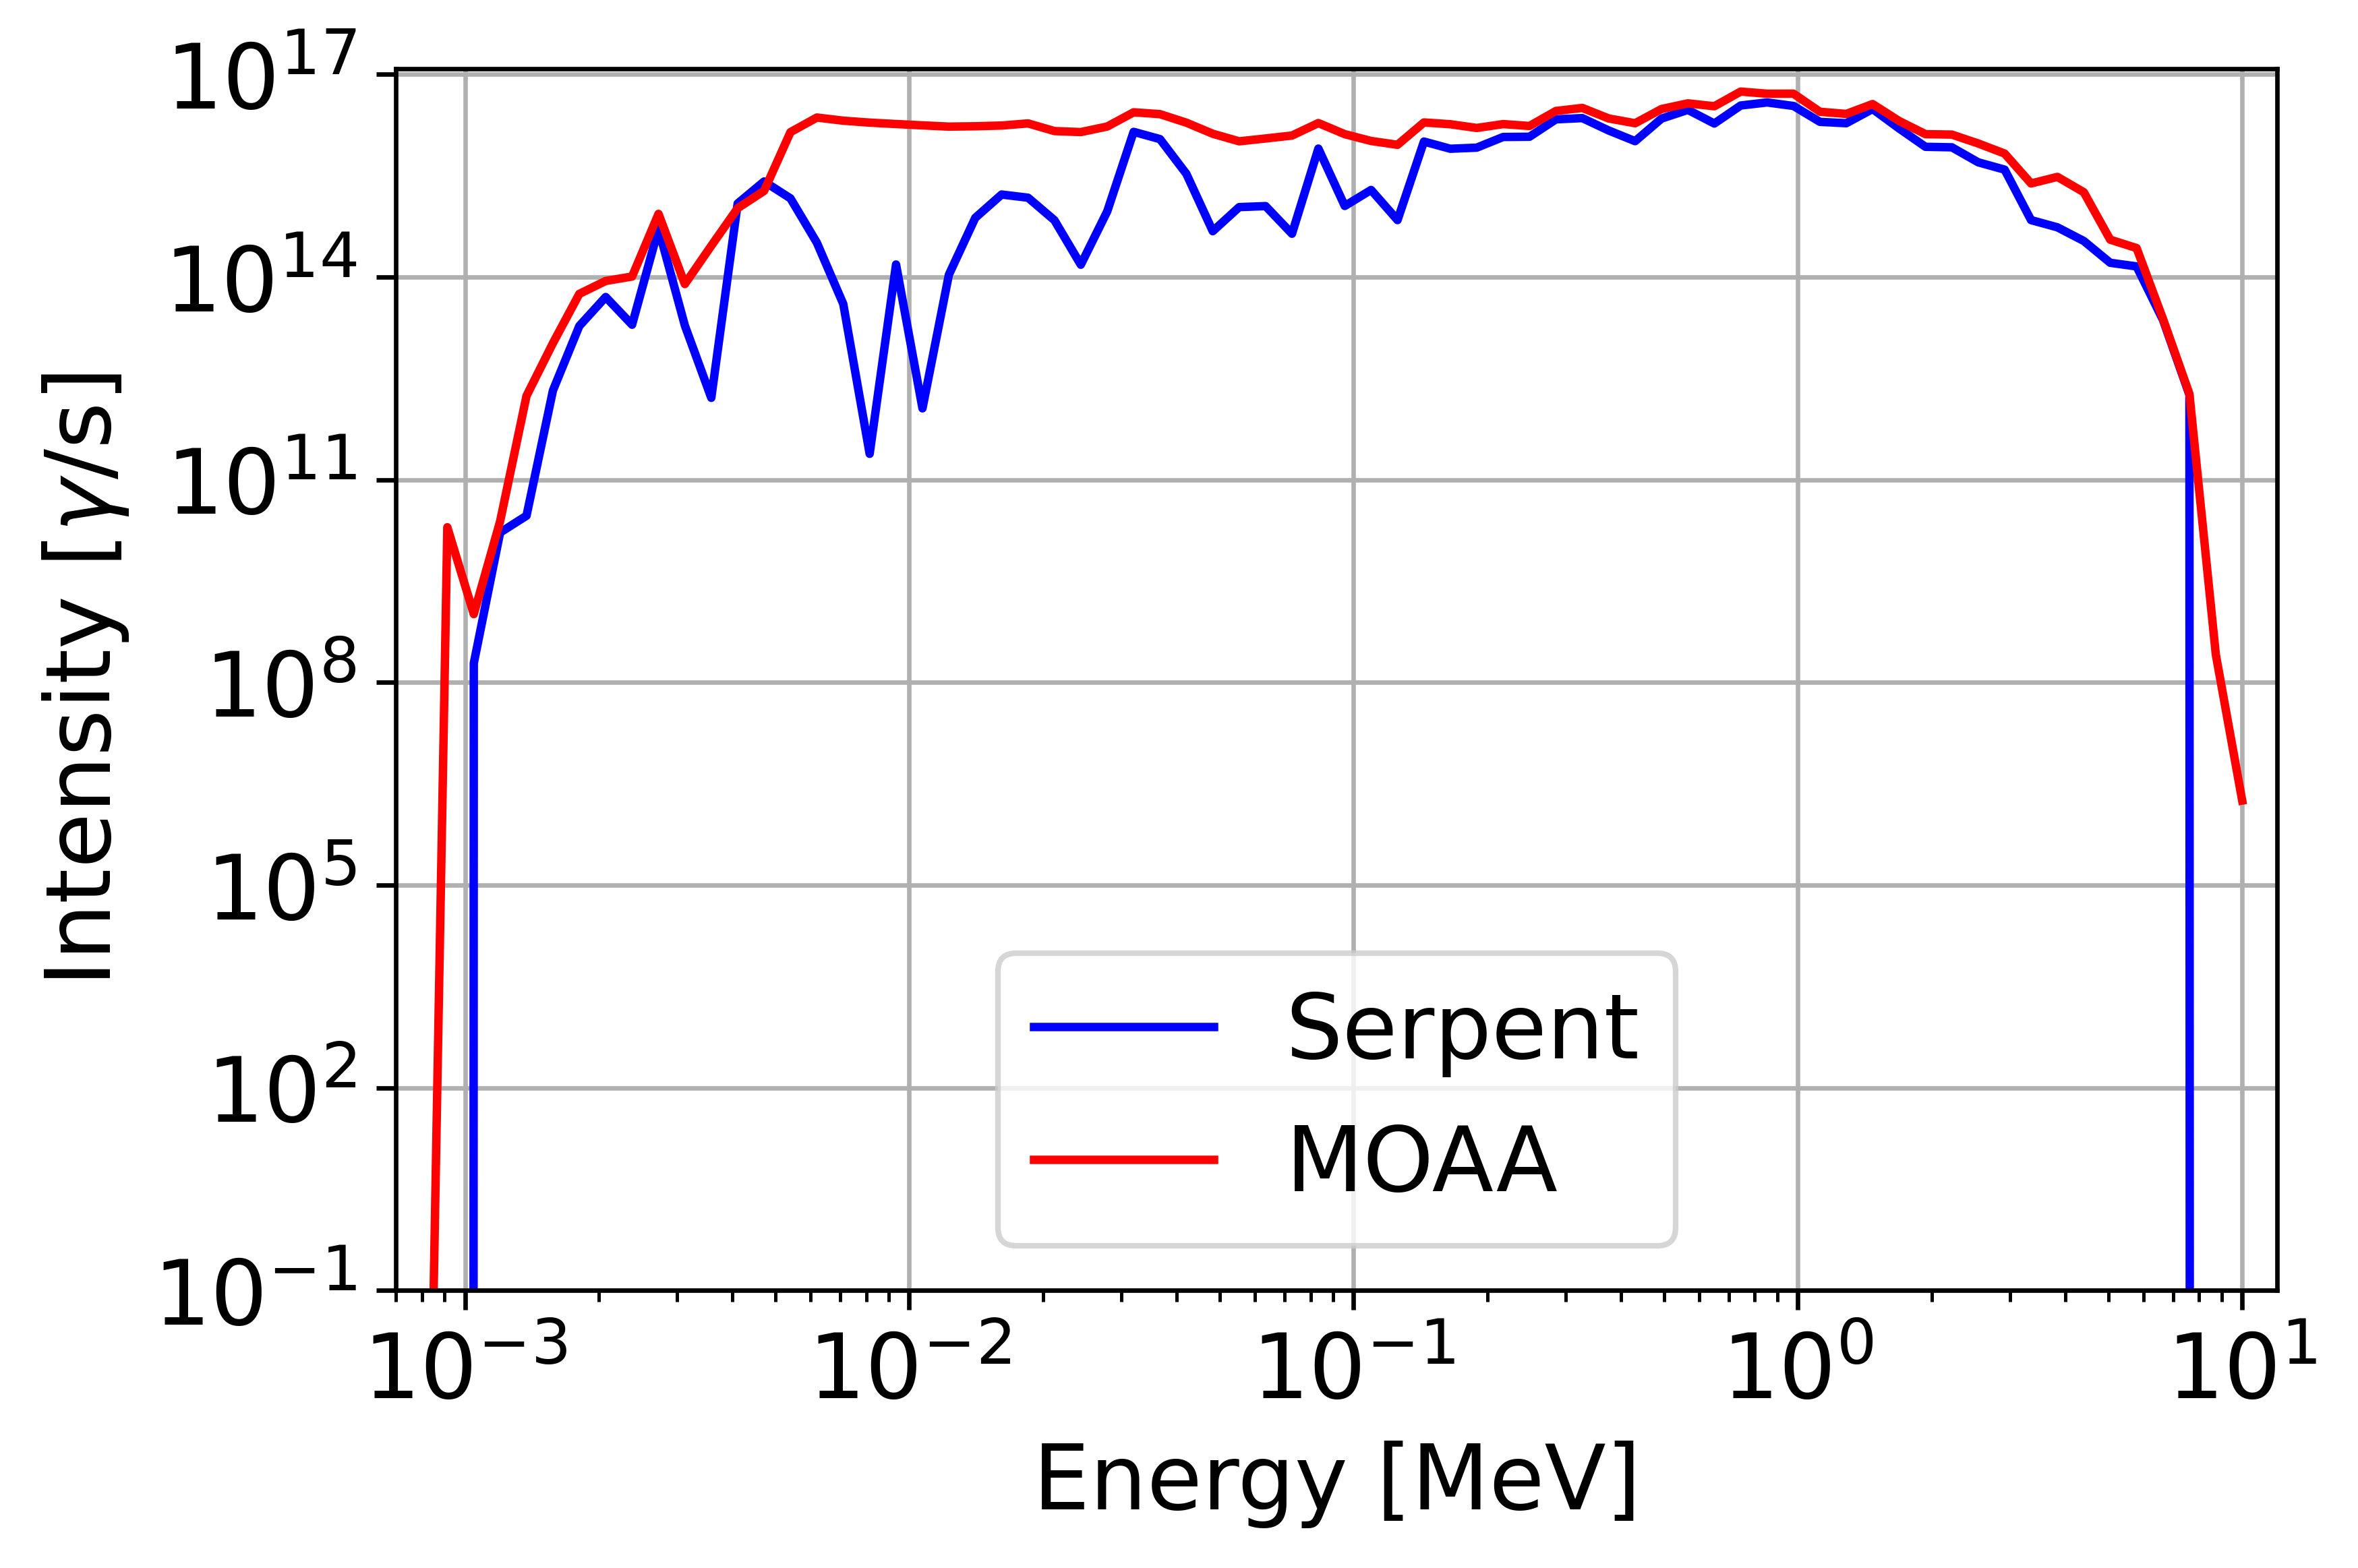
\includegraphics[width=0.6\linewidth]{figures/g-source.png}
    \hfill
    \caption{MOAA and Serpent photon source distributions.}
    \label{fig:g-source}
\end{figure}

Figure \ref{fig:g-spectra} displays the gamma spectra.
The largest discrepancy in the spectra is close to 10 keV.
MCNP fails to resolve some of the peaks in that area.
Additionally, the differences in gamma source distributions are carried over. 
Table \ref{tab:gam-heat-results} shows the results for the total gamma flux and the gamma heating.
Overall, the MCNP results are approximately 50\% larger than Serpent's.

Calculating the gamma heating per source particle, we can isolate the effects of the source intensity and source energy distribution on the results.
$H_{\gamma, Tr}/source$ in Table \ref{tab:gam-heat-results} shows the effects of the source energy distribution.
The MCNP value is 30\% smaller than Serpent's.
This last result confirms that the discrepancies in the total gamma flux and gamma heating are caused by the differences in both the source energy distribution and the source intensity.

% Gamma spectra
\begin{figure}[htbp!] %or H 
    \centering
    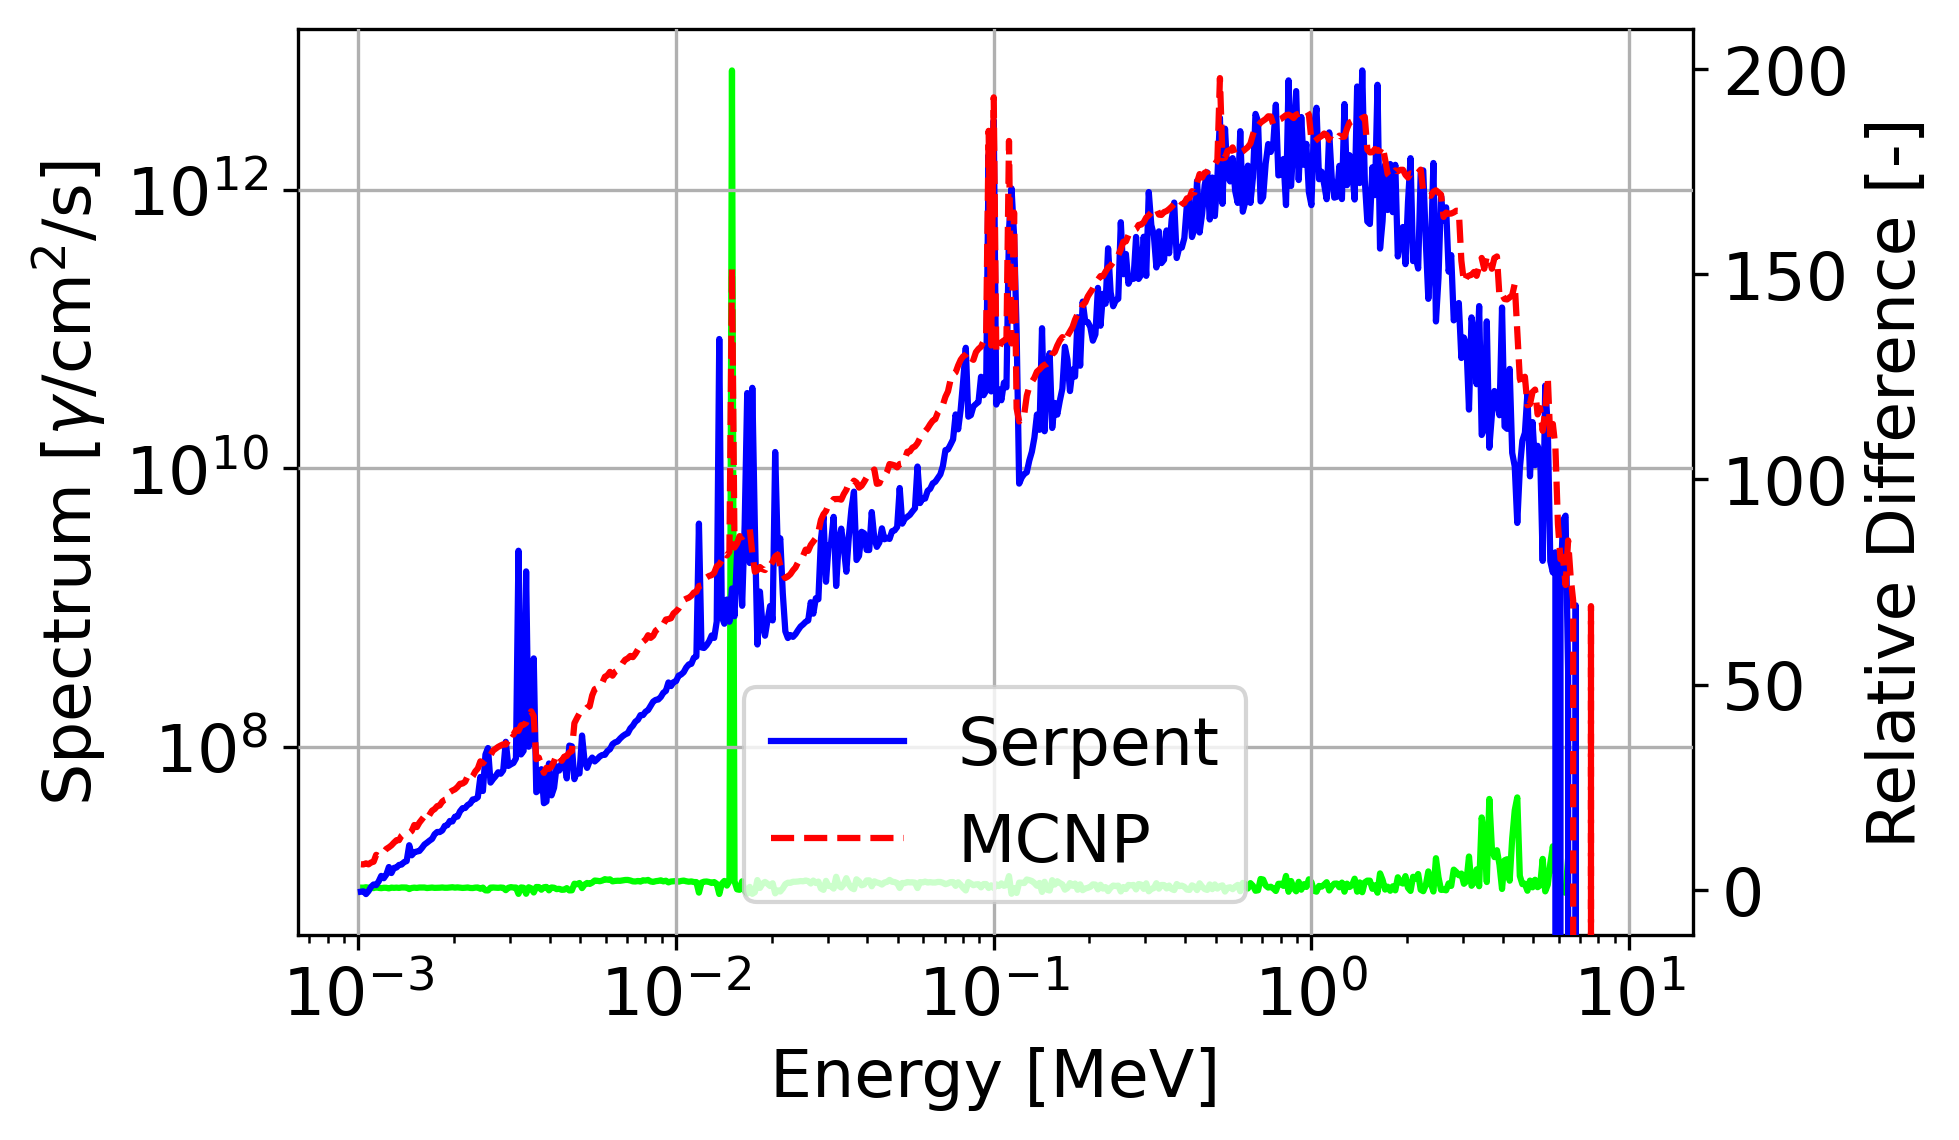
\includegraphics[width=0.65\linewidth]{figures/g-spect.png}
    \hfill
    \caption{MCNP and Serpent photon spectra.}
    \label{fig:g-spectra}
\end{figure}


\subsection{Demonstration Problem}
\label{sec:demo}
% From 14-

A top view of the exercise geometry and its dimensions are shown in Figure \ref{fig:toy-geo}.
The experiment center is located 8.2 cm away from the reactor center.
The fuel element and experiment heights are 14.8 and 24 cm, respectively.
The reactor encompasses the following materials: 85\% enriched uranium with a density of 19 g/cm$^3$ for the fuel elements, light water with a density of 1 g/cm$^3$ for the moderator, and iron with a density of 7.87 g/cm$^3$ for the experiment.

\begin{figure}[htbp!] %or H 
    \centering
    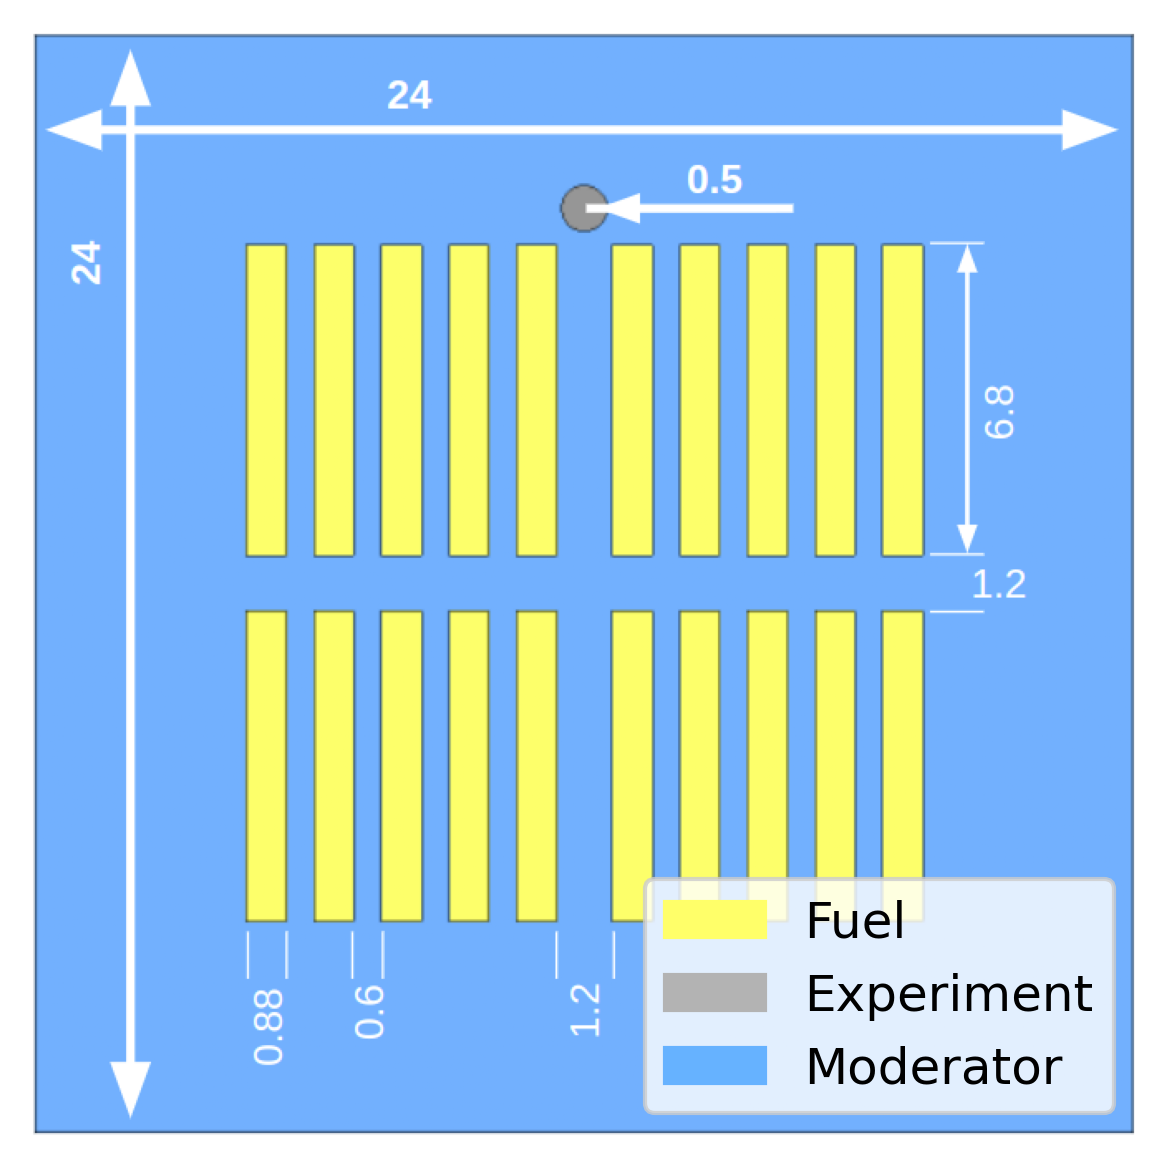
\includegraphics[width=0.50\linewidth]{figures/neutronics2-geo-legend}
    \hfill
    \caption{Geometry of the demonstration problem.}
    \label{fig:toy-geo}
\end{figure}

The experiment is irradiated for a period of 50 days with the reactor operating at a constant power of 5 MWth.
% TODO: Cross-section libraries?
After that period, the reactor shuts down, and the heat deposited in the experiment is calculated immediately after shutdown (to avoid the prompt-gamma contributions, this step is taken 1 sec after shutdown).
The reactor regions considered to contribute to the experiment heating are the fuel elements and the same experiment, while the activation of the moderator is neglected.


% This two figures could be grouped together
% total heating over time
\begin{figure}[htbp!] %or H 
    \centering
    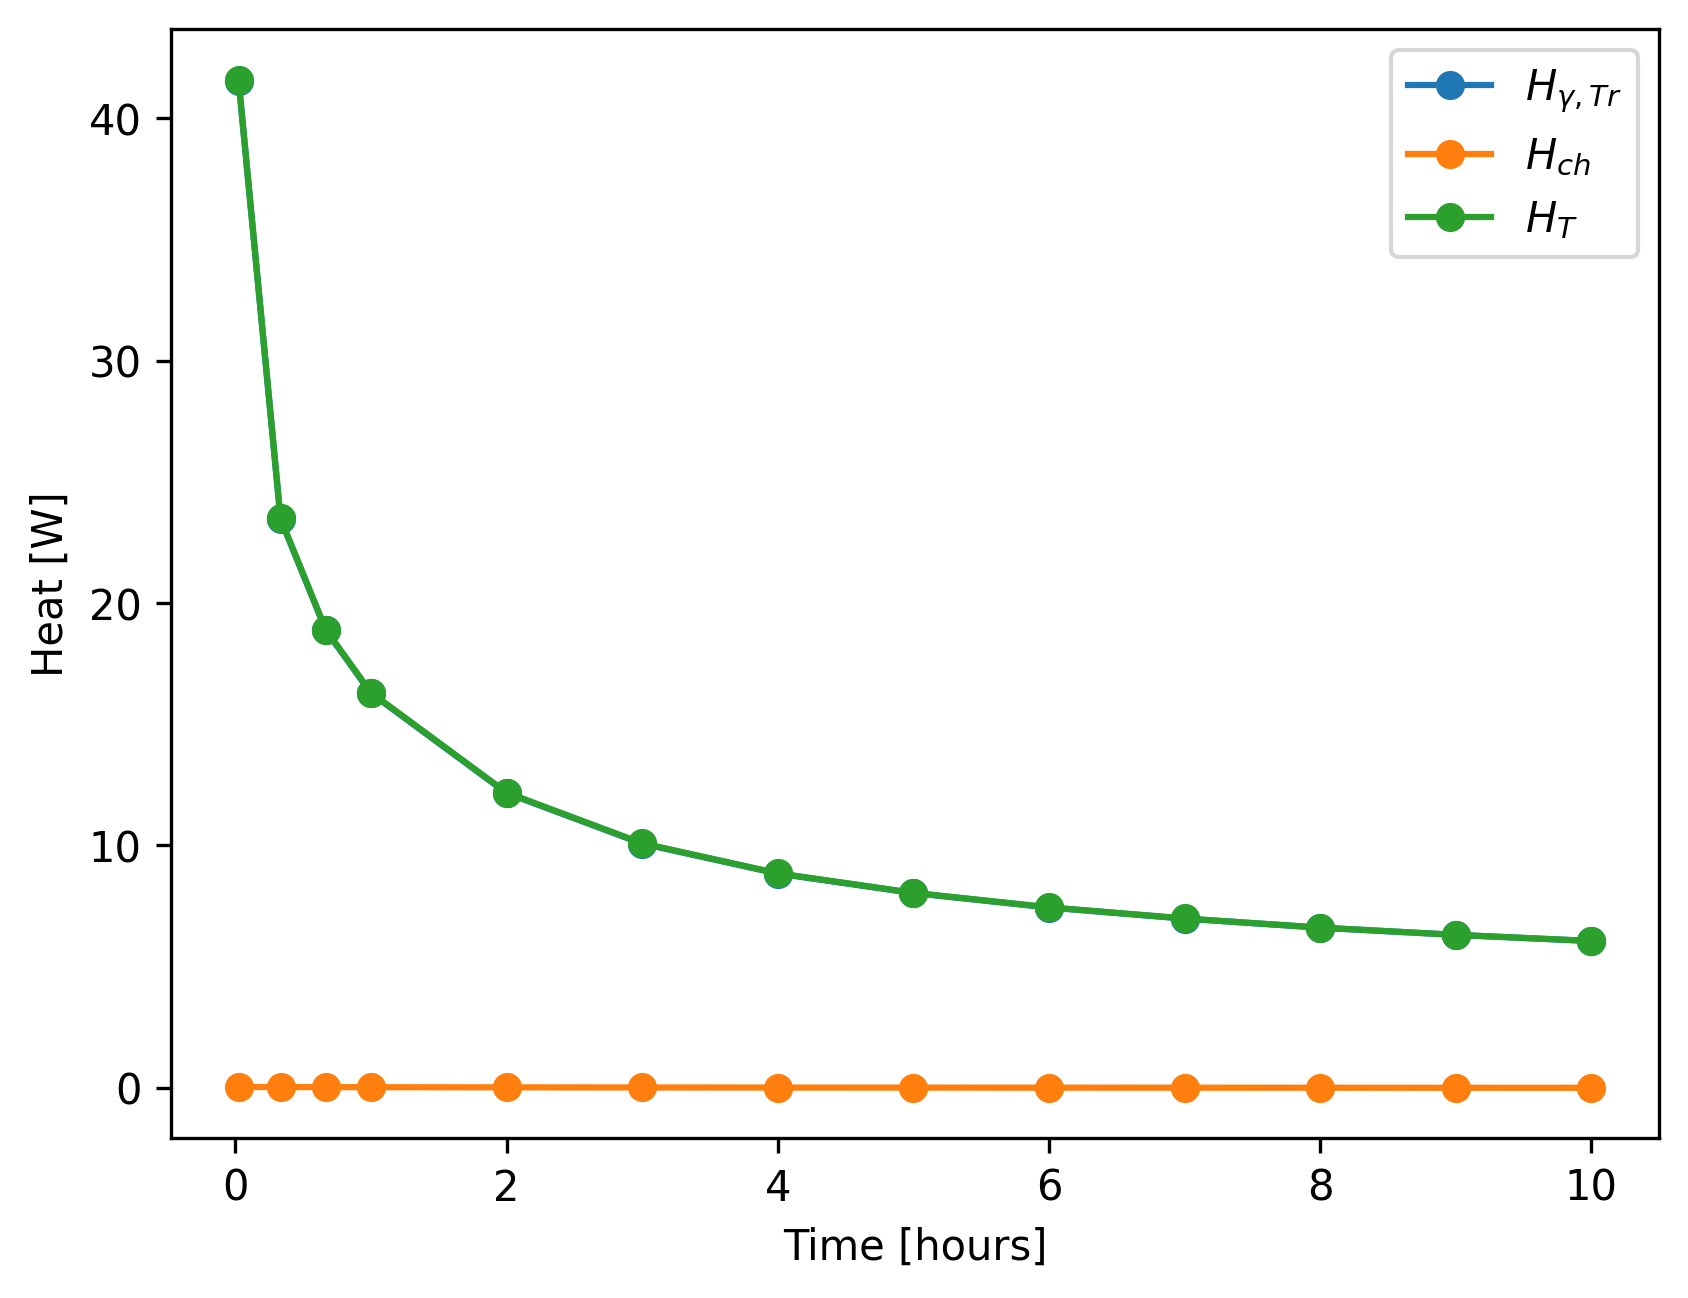
\includegraphics[width=0.55\linewidth]{figures/reference-decay-over-time}
    \hfill
    \caption{Heat production in experiment over time for the demonstration exercise.}
    \label{fig:demo-time}
\end{figure}

Figure \ref{fig:demo-time} displays the heat production over time in the experiment.
The heat produced in the experiment immediately after shutdown is 41.58 W, which is less than 0.001\% of the reactor total power.
As expected, the heat deposition has a decaying shape.
The curve has a half-life lower than 1 second, and after 4 seconds the heat production becomes smaller than 10 W.

% heat contribution by source
\begin{figure}[htbp!] %or H 
    \centering
    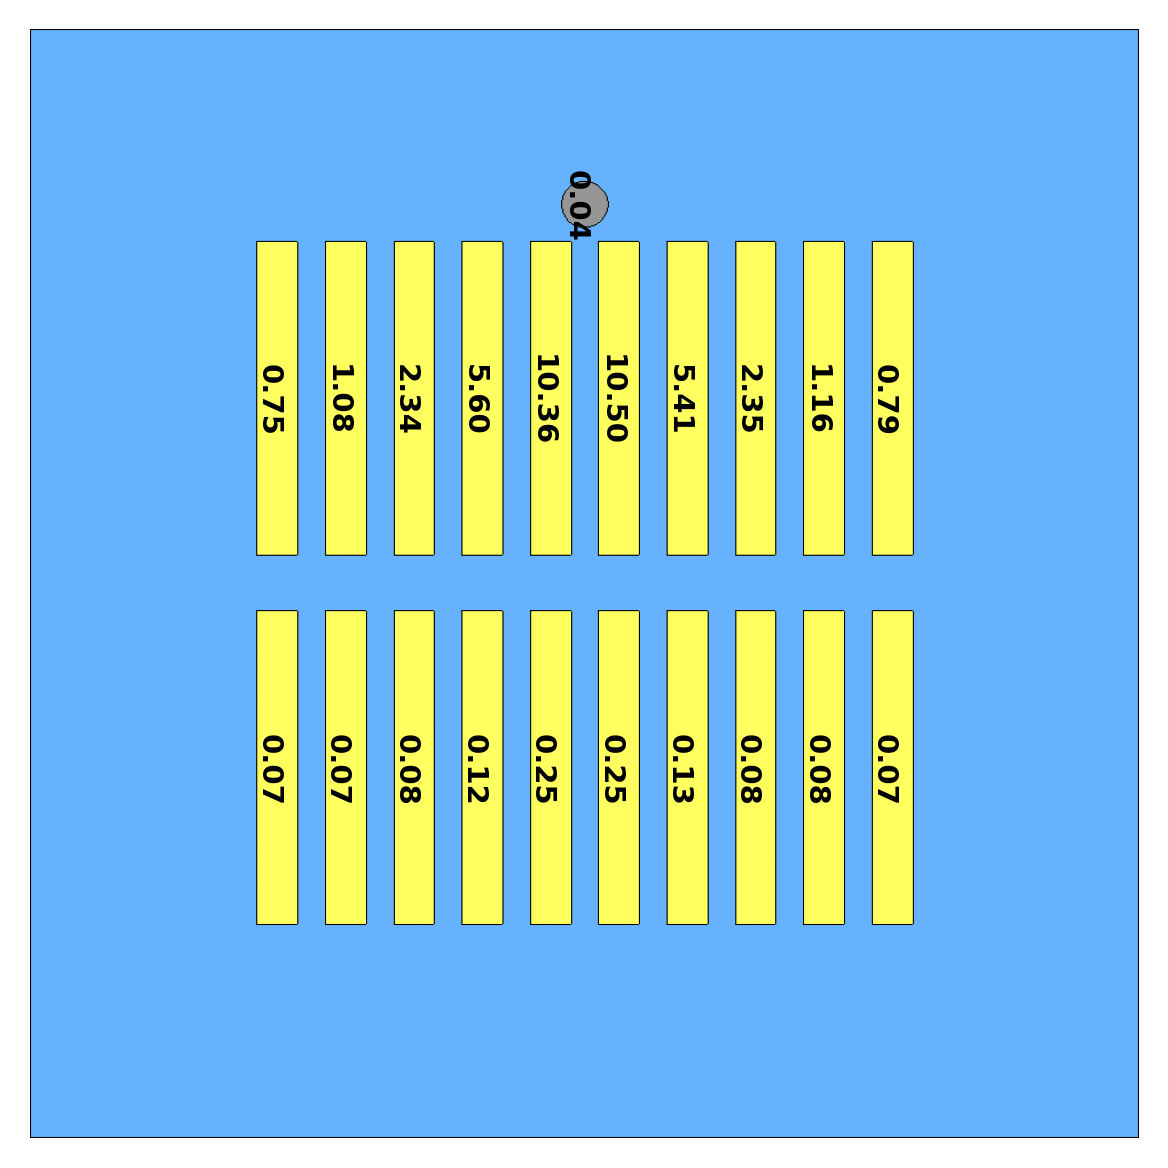
\includegraphics[width=0.70\linewidth]{figures/reference-contribs}
    \hfill
    \caption{Heat contribution by each source immediately after shutdown. Values expressed in \textit{W}.}
    \label{fig:demo-contrib}
\end{figure}

Figure \ref{fig:demo-contrib} shows the heat contribution by source.
The fuel elements contribute to the experiment heating via the deposition of the gamma radiation that originates in them.
The largest contribution to the heat deposition is originated in the closest fuel elements to the experiment.
The experiment self-heating is a combination of the energy deposition of the charged particles and gamma radiation originating in the same experiment.
The experiment material is not considerably activated during the irradiation period, and the self-heating contribution is deemed negligible.


\subsection{ATR experiment}
\label{sec:atrexp}

% % TO INCLUDE SOMEWHERE:
% % tomberlin_advanced_2002
% Two general types of experiments:
% A pressurized water loop (PWL) type of experiment that circulates water at typical pressure and temperature of an LWR.
% Capsule experiments irradiated inside the reactor pressure vessel, which rely on the reactor primary coolant for heat dissipation.

% Capsules may be any length up to 122 cm.

% % noauthor_i-loop_2019
% (1) pressurized water loop in-pile tube (IPT) experiment assemblies,
% (2) drop-in capsule irradiation assemblies
% (3) instrumented lead capsule assemblies.

% The first experiment type is positioned in an IPT that isolates the experiment from the reactor coolant and provides a way to control the experiment environment in terms of pressure, temperature, coolant flow, and chemistry.
% The second is a drop-in capsule fixed in a core or a capsule irradiation tank position and cooled by reactor primary coolant.
% The third type is a lead capsule experiment fixed in a core or a capsule irradiation tank position with instrumentation lines that exit the experiment and the reactor vessel and are connected to a control system for monitoring and controlling operating parameters.

% Intro - Why do we care about this.
The calculation scheme presented in this work is reactor-agnostic, meaning that it can be tailored to any research reactor.
Section \ref{sec:demo} calculated the delayed heating in a simple configuration, which eases the visualization of the calculation scheme.
This section demonstrates the calculation scheme for a full-scale research reactor, the \gls*{ATR}.

% ATR: Intro
The \gls*{ATR} is a 250-MWth high flux test reactor located at the Reactor Technology Complex of the \gls*{INL}.
The ATR was designed to provide an irradiation test environment for conducting a variety of experiments, to study the effects of radiation on reactor structural and fuel materials, and to produce medical and industrial isotopes \cite{ICSBEP, tomberlin_advanced_2002}.

% ATR: reactor description
The ATR core contains 40 fuel elements arranged in a serpentine annulus between and around nine flux traps, as shown in Figure \ref{fig:atr}.
Each fuel element consists of 19 parallel, curved, aluminum-clad fuel plates forming a 45-degree sector of a right circular cylinder.
The fuel arrangement gives the reactor core a clover-leaf configuration, which allows the \gls*{ATR} to be operated at different power levels in the corner lobes, allowing for independent testing conditions within the same operating cycle.
Within each fuel plate, the fuel meat consists of highly enriched (93 wt\%) uranium aluminide (UAl$_x$) fuel powder dispersed in aluminum.
Plates 1 through 4 and 16 through 19 contain natural boron carbide (B$_4$C) powder as a burnable poison.

% ATR figure of the model
\begin{figure}[htbp!] %or H 
    \centering
    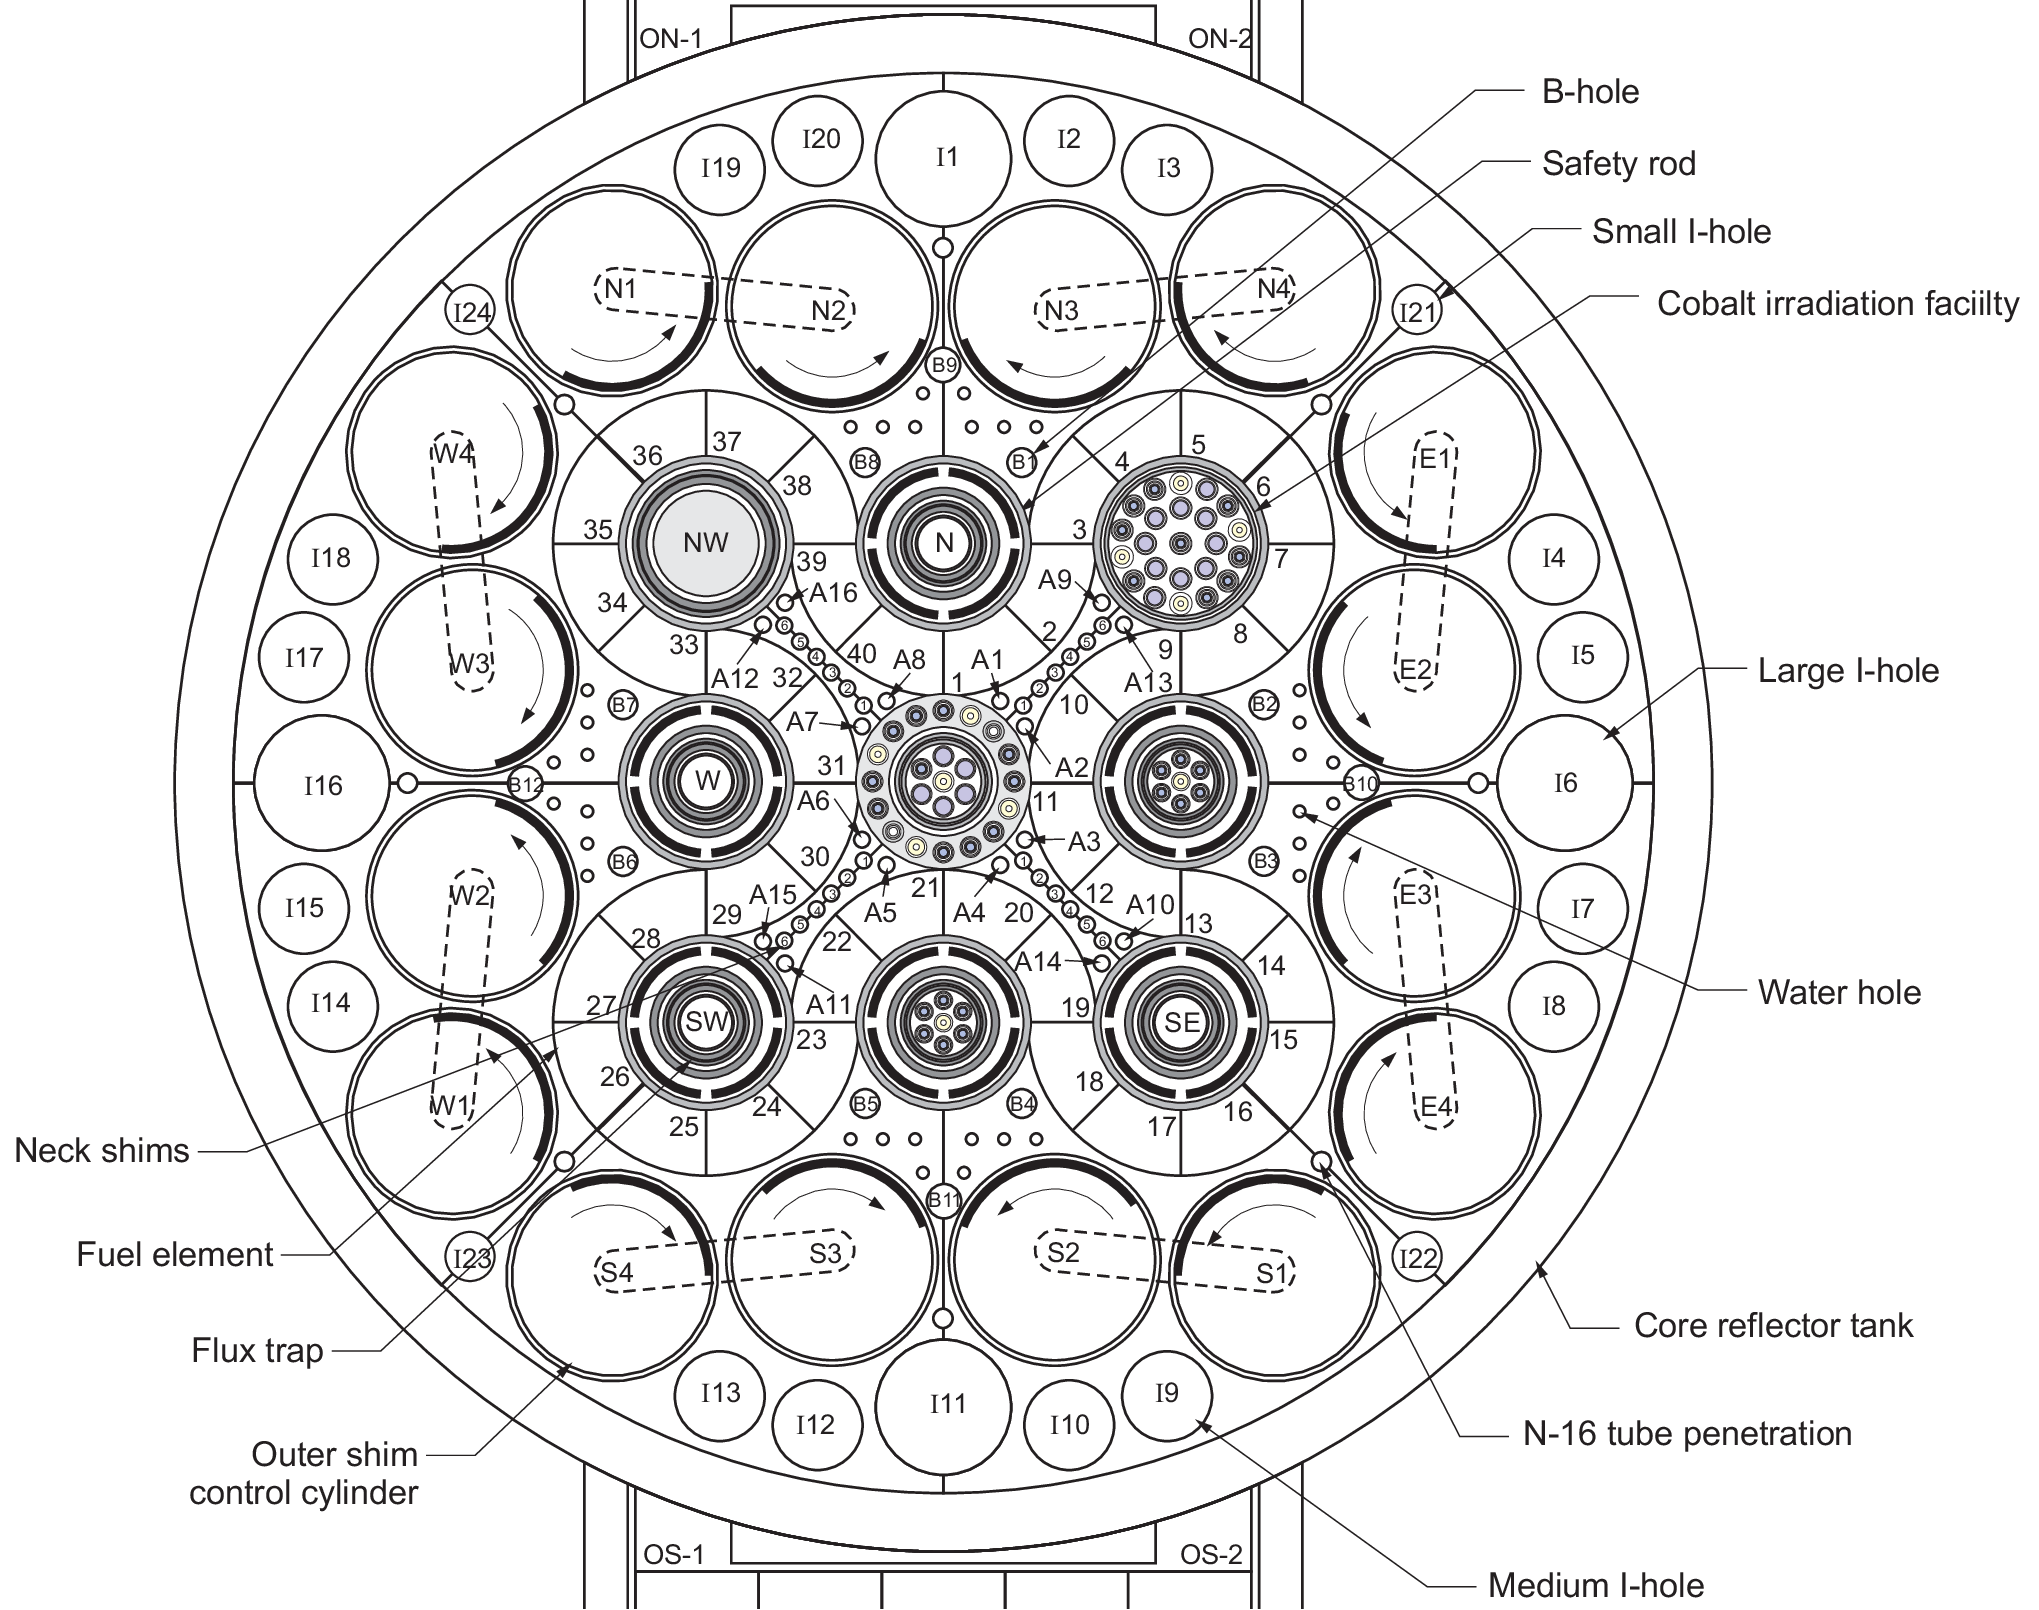
\includegraphics[width=0.85\linewidth]{figures/atr2}
    \hfill
    \caption{Top view of the ATR. Image reproduced from \cite{ICSBEP}.}
    \label{fig:atr}
\end{figure}

% Experiment positions
The reactor has 9 flux trap positions and 68 additional irradiation positions inside the reactor core reflector tank.
The center capsule facility is surrounded by the H-hole irradiation facility, which contains 10 cobalt baskets, 4 flux monitor holders, and 2 N-16 flow tubes.
The neck shim housing is the structural guide for the 24 neck shim and regulating rods, as well as 8 inner and 8 outer A-holes.
The beryllium reflector fills the space between the fuel annulus and the core reflector tank, and it hosts the outer shim control cylinders (OSCC), irradiation holes, and water holes.
The irradiation holes include a total of 8 small B-holes, 4 large B-holes, 4 small I-holes, 16 medium I-holes, 4 large I-holes, and 4 round and 4 square N-16 monitor holes.

% Describe model
This work uses an MCNP model representing the ATR critical experiment evaluation designated as Cycle 103A-2 that was performed in 1994.
This critical evaluation was part of a nuclear re-qualification program that followed the core internals change-out.
The critical configuration was defined by the following parameters: 40 fresh fuel elements, OSCC set to 51.8 degrees, 22 shim rods fully inserted, 2 regulating rods fully withdrawn, and 6 safety rods fully withdrawn.

The ATR critical evaluation was published by the OECD NEA Nuclear Science Committee in the September 2005 Edition of the International Handbook of Evaluated Criticality Safety Benchmark Experiments (ICSBEP Handbook) \cite{ICSBEP}.
% ATR-FUND-RESR-001 was approved by the IRPhEP in October of 2008 and is published in the International Handbook of Evaluated Reactor Physics Benchmark Experiments under its ICSBEP Identifier, HEU-MET-THERM-022.
% % The report is published in the original ICSBEP format and contains only evaluation of the critical state measurement.
The original benchmark model uses the evaluated continuous energy ENDF/B-V cross-section data for 27 $^{\circ}$C.
% TODO/MAYBE: make sure that I am using this cross-section library
This work uses the ENDF/B-VIII.0 cross-section library for the isotopes included in it.
The remaining isotopes use the cross-section data of the original model.
% The benchmark model 
The model uses 10$^4$ histories per generation with 250 and 3750 inactive and active cycles.
This work considers the reactor composition at the \gls*{BOC} based on the available ATR model.

% Problem definition
This demonstration exercise focuses on the delayed heating of the A1 experiment position.
The A1 experiment position is an inner A-hole, and it is hosted by the neck shim housing.
The diameter of the hole is 0.625 in.
This exercise considers an experiment sample made of aluminum.

% POWER
Although the ATR maximum power rating is 250 MWth, most contemporary experiments do not require such a level, and the reactor operates at a much lower power.
This work considers for the calculations a total operating power of 110 MWth that is equally distributed among the 5 lobes.
% Irradiation time
The irradiation time is 30 days, and the decay is recorded in seven non-uniformly distributed steps up to 12 hours after shutdown.
% This work considers the reactor composition at the \gls*{BOC} based on the available ATR model.
% However, nuclear heating tends to increase throughout the core depletion \cite{ilas_impact_2013}.
% A more conservative approach would then use the \gls*{MOC} or \gls*{EOC} configurations.

% Contributing cells
As the experiment position is in the core region between the fuel assemblies, the calculations assume that the fission products generate a much higher gamma source intensity than the activation products in the neighboring cells.
Hence, the contribution of the reactor components surrounding the experiment is neglected.
The only considered contributors to the heating are all the fuel plates and the experiment itself.


% ATR results
\subsection{ATR results}

% CHANGES IN MCNP INPUT
To accommodate the MOAA calculations, the MCNP input file underwent the following modifications.
The ATR model defines 19 different material compositions that all fuel elements share for their 19 different fuel plates.
The material definitions of each fuel plate were duplicated for each fuel element to allow for their independent definition.
Additionally, the volume of each fuel plate was calculated and added into the MCNP input file.

Figure \ref{fig:atr-time} presents the experiment heat production over time.
$H_{\gamma,Tr}$ was calculated for 41 independent photon-transport simulations, wherein each simulation accounts for the contribution to delayed gamma heating of each fuel assembly and the experiment itself.

The gamma heating immediately after shutdown was 849.2 W, and the heating due to charged particles was 56.32 W, which equals to 6.6\% of the total heating in the experiment.
The self-gamma heating was 5.8 W, which is equal to 0.73\% of the total delayed gamma contribution and 0.68\% of the total heating.
These results show that the self-heating in aluminum is very low and validate the initial simplification of neglecting the surrounding structure contributions given that both the experiment and the structures are made of aluminum.

Additionally, the heating due to charged particles decays much faster than the gamma heating and becomes negligible one hour after shutdown.
The gamma heating decays to 100 W at approximately six hours after shutdown.

\begin{figure}[htbp!] %or H 
    \centering
    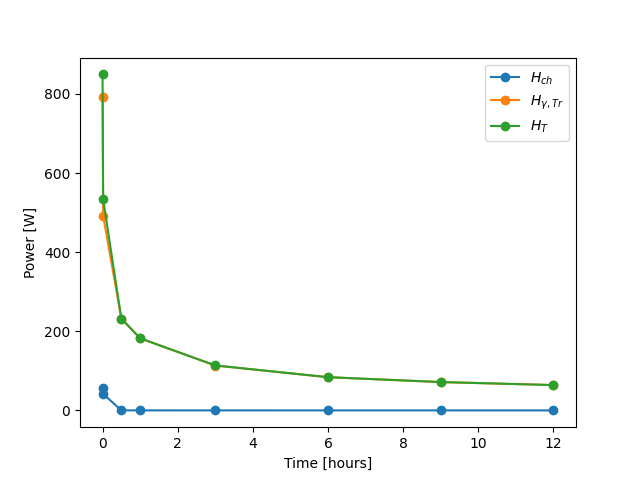
\includegraphics[width=0.65\linewidth]{figures/atr-decay-heat-time}
    \hfill
    \caption{Shutdown heating rate over time in the ATR A1 experiment position for an aluminum sample.}
    \label{fig:atr-time}
\end{figure}

Figure \ref{fig:atr-contrib} shows the contribution to the total heat in percentage by each fuel assembly and the experiment immediately after shutdown.
The largest contributions to the heating in the sample come from the fuel assemblies 1, 10, 40, 2, 11, 9 with contributions of more than 3\%.
These assemblies are the closest in distance to the experiment position.
Additionally, the sample produced a self-heating of 7.3\%, from which 6.6\% came from the charged particles, and 0.7\% from the gamma particles.
% This confirms the assumption that the gamma heating from the fission products is considerably larger than the gamma heating from activation products in the vicinity of the fuel assemblies.

% Maybe talk about the following:
% The neck shim housing has an elongated shape.
% So, several of the gammas originated here will not be deposited in the experiment position but in the fuel elements.
% Additionally, our method considers that the gamma are originated uniformly across the cell geometry.
% Which in this case a mesh based approach may be more accurate.

\begin{figure}[htbp!] %or H 
    \centering
    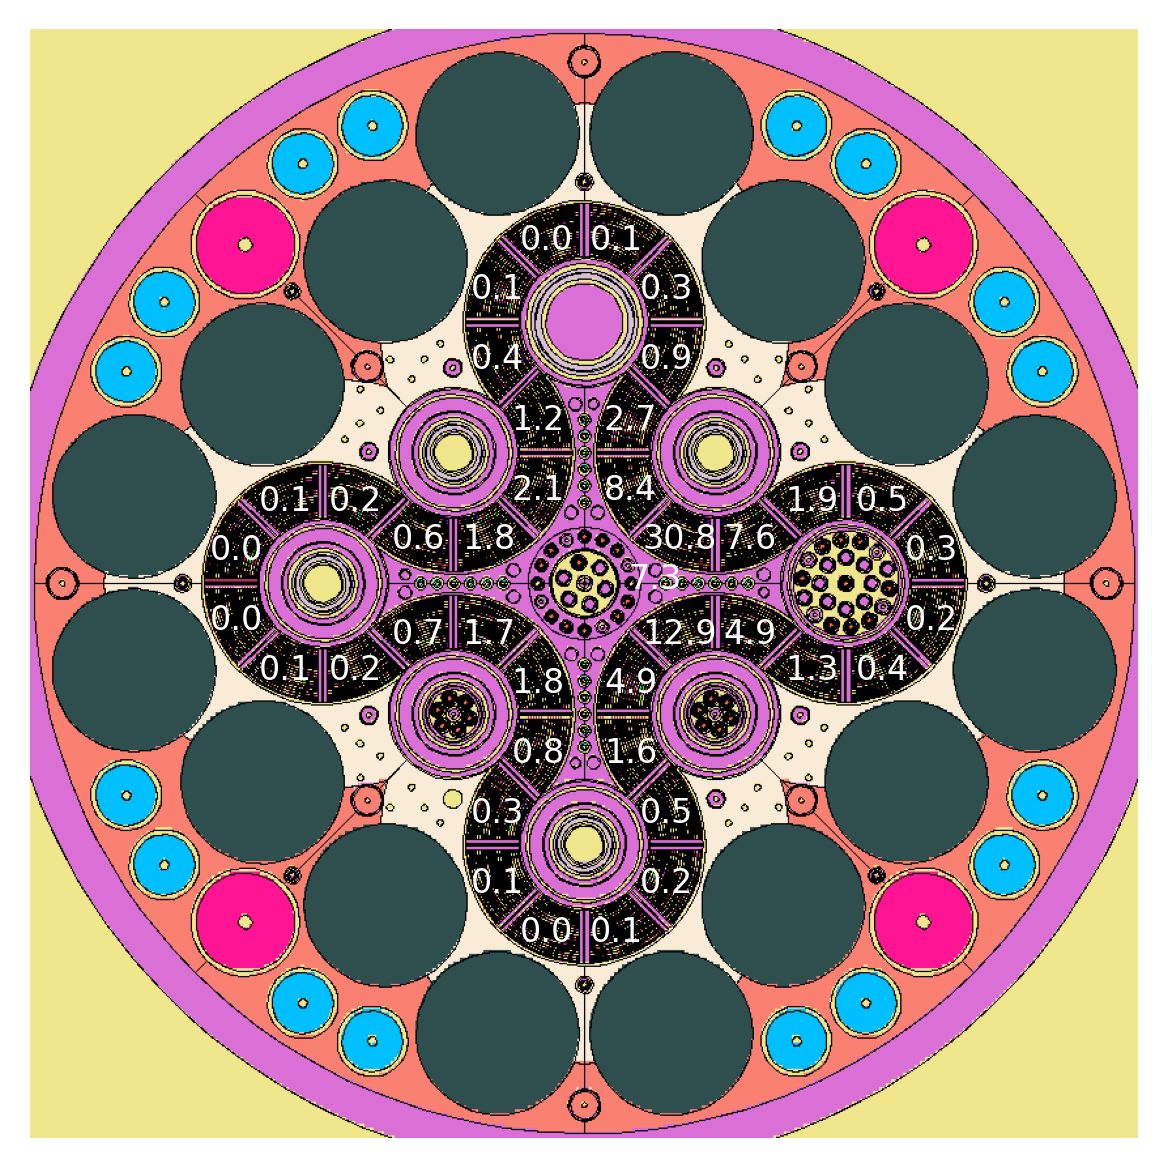
\includegraphics[width=0.90\linewidth]{figures/atr-contributions}
    \hfill
    \caption{Contribution by each source to the A1 experiment heat rate immediately after reactor shutdown, with the values expressed in (\%). The Figure is based on the MCNP model geometry, which is rotated 45$^{\circ}$ clockwise with respect to Figure \ref{fig:atr}.}
    \label{fig:atr-contrib}
\end{figure}


\subsection{RA-6 structures}

% Intro
The RA-6 is a 3-MWth open pool research reactor located at the Bariloche Atomic Center (CAB), a research and development center of the Argentine National Atomic Energy Commission (CNEA) \cite{ICSBEP}.
It was originally conceived as a teaching tool to support student training at the Balseiro Institute before its uses became diversified.
Current applications include neutron activation analysis, neutron radiography, and \gls*{BNCT}, among others.

% The reactor
The reactor core is composed of a fuel element arrangement, as shown in Figure \ref{fig:ra6-1}, that rests on a support grid inside a 2.4-m-diameter, 10.4-m-high stainless-steel tank.
The tank is filled with demineralized light water, which acts as a coolant, moderator, and reflector.
The fuel elements are Material Test Reactor (MTR) type, composed of rectangular fuel plates with aluminum side plates.
The fuel meat consists of 19.7\% enriched uranium silicide (U$_3$Si$_2$) dispersed in an aluminum matrix.
There are two types of fuel elements: Normal Fuel Elements (NFEs) and Control Fuel Elements (CFEs).
While an NFE is composed of 17 internal and two external fuel plates, a CFE is composed of 14 internal and 4 control guide plates.

% Support grid
The bottom plane of the core assembly rests 8.9-meters-deep on the support grid, which is a 20 cm-thick slab of 99.5\% pure aluminum.
Primary and secondary cylindrical holes allow the cooling of the internal and external fuel plates, respectively.
The primary holes have a diameter of 6.179 cm and are arranged in a rectangular 8x10 array with 7.7-cm pitch in the x-direction and 8.1-cm pitch in the y-direction.
The secondary holes have a diameter of 2.225 cm and are centered between the primary holes.

% BNCT filter
On a side of the fuel element arrangement, there is a neutron filter that works as a source for \gls*{BNCT}, as shown in Figure \ref{fig:ra6-2}.
The neutron filter for the \gls*{BNCT} facility is an 87.6-cm-long, 77.1-cm-wide, 82.35-cm-high aluminum container.
The filter is filled along the 87.6-cm dimension with the following materials: 17 cm of aluminum bricks, a 0.15-cm-thick cadmium sheet, 10 cm of aluminum, a 0.15-cm-thick cadmium sheet, and the rest is filled with alumina bricks.

\begin{figure}[htbp!] %or H 
    \centering
    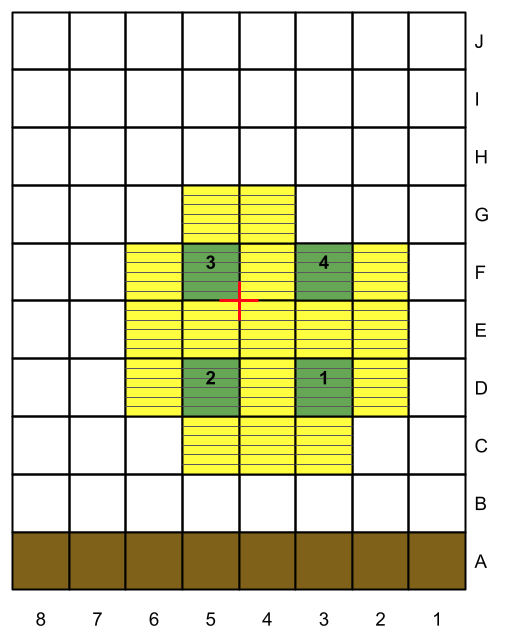
\includegraphics[width=0.50\linewidth]{figures/ra6-core2}
    \hfill
    \caption{Top view of the RA-6 critical configuration. NFEs in yellow, CFEs in green, and BNCT filter in brown. Red cross denotes the center of the reactor pool. Image reproduced from \cite{ICSBEP}.}
    \label{fig:ra6-1}
\end{figure}

\begin{figure}[htbp!] %or H 
    \centering
    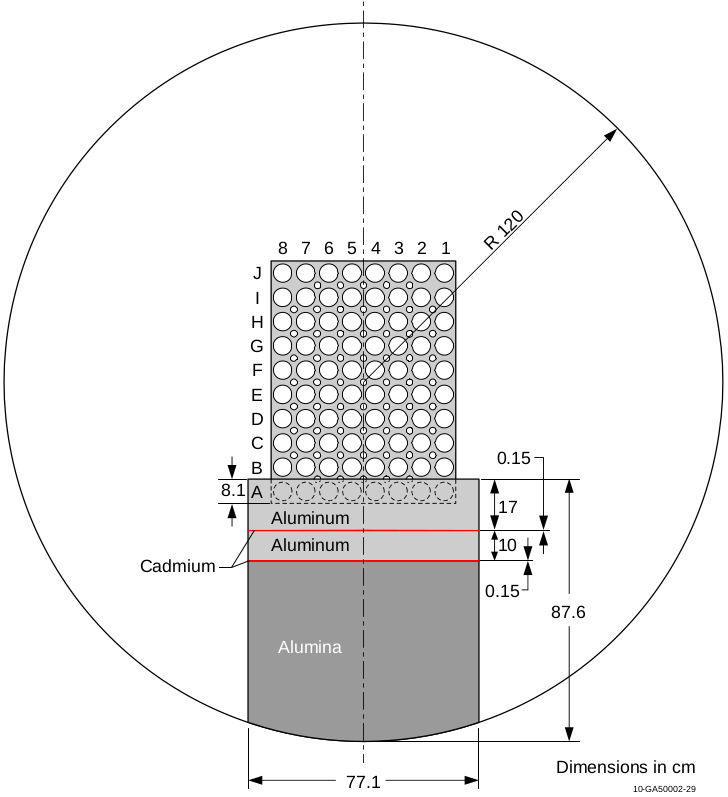
\includegraphics[width=0.65\linewidth]{figures/bnct}
    \hfill
    \caption{Top view of the RA-6 support grid and BNCT filter. Image reproduced from \cite{ICSBEP}.}
    \label{fig:ra6-2}
\end{figure}

% The model
The RA-6 reactor operated for 20 years with spent \gls*{HEU} fuel from a higher power reactor and was converted to \gls*{LEU} fuel in 2008.
The RA-6 critical experiment reported in this evaluation corresponds to the 2008 configuration utilized in the startup program.
% RA6-FUND-RESR-001 
This critical evaluation was published by the OECD NEA Nuclear Science Committee in the September 2010 Edition of the ICSBEP Handbook.
% RA6-FUND-RESR-001 was first published by the IRPhEP in the March 2013 Edition of the International Handbook of Evaluated Reactor Physics Benchmark Experiments under its ICSBEP Indentifier, IEU-COMP-THERM-014.
% The report contains only an evaluation of the critical state measurement.
This work considers the reactor composition at the \gls*{BOC} based on the available RA-6 model and uses the evaluated continuous energy ENDF66 cross-section data for 27 $^{\circ}$C, which is defined in the original benchmark model.
% % TODO/MAYBE: make sure that I am using this cross-section library
% This work uses the ENDF/B-VII.1 cross-section library for the isotopes included in it.
% The remaining isotopes use the original model cross-section data.
% The benchmark model 
The simulation uses 10$^4$ histories per generation with 50 and 4000 inactive and active cycles.

% The calculations
Although not shown in the MCNP model, the reactor core has several surrounding components, such as primary pipes, the stainless-steel tank, and neutron beam extraction tubes.
The analysis of delayed heating in these components could be worthwhile but was omitted as the MCNP model excluded them.
Hence, this work calculates the delayed heating on the most important structural components in the model, i.e., the support grid and the BNCT filter.

% POWER
The RA-6 was originally designed to operate at 1 MWth and the 2008 startup program included a reactor power upgrade to 3 MWth.
Although the RA-6 maximum power rating is 3 MWth, it normally operates at a lower power.
This work considers operating powers of 1 and 3 MWth and compared their respective results.
% Irradiation time
In this work, the rector operated for 1 year and the depletion was calculated in four 3-month steps.
% Contributing cells
The considered contributors to the heating are the fuel plates, the support grid, and the BNCT filter.


\subsection{RA-6 results}

% CHANGES IN MCNP INPUT
To accommodate the MOAA calculations, the MCNP input file underwent the following modifications.
First, even though the RA-6 model distinguishes between five different types of fuel plates: internal plates in the nuclear fuel elements (NFEs), internal plates with burnable poisons in the NFEs, external plates in the NFEs, fuel plate with burnable poisons in the control fuel elements (CFEs), and fuel plate without burnable poisons in the CFEs, the original MCNP input file defines all of them with the same material definition.
Additionally, several layers of the BNCT filter and the support grid are made of pure aluminum, and the original MCNP input file defines the material aluminum only once.
The BNCT filter also uses two cadmium layers that share the same material definition in the original MCNP input file.
All material definitions of these components were duplicated to allow for their independent definition.
Second, the original MCNP input file defines the four CFEs using nested structures with independent cells, but as their definition is identical, a minimal universe renumbering allowed for their simultaneous modeling in MOAA.
Third, the volume of each fuel plate type, the volume of the different BNCT filter layers, and the volume of the support grid were calculated and added into the MCNP input file.

Figure \ref{fig:ra6-3} shows the delayed heating in the support grid and the different BNCT filter layers for operating powers of 1 and 3 MWth, and Table \ref{tab:ra6-res} shows the deposited heat density in the different structures.
The highest deposited heat occurs in the first BNCT layer, while the highest deposited heat density occurs in the second BNCT layer, which is the first cadmium layer in the filter.
For the first, third, and fifth layers of the BNCT filter, the deposited heat density decreases due to an increase in the spatial distance from the core.
However, the fifth layer has a larger deposited heat than the third layer due to its considerably larger volume.
The deposited heat in the cadmium sheets is considerably smaller than for the rest of the BNCT layers due to their smaller volume.
Table \ref{tab:ra6-res} also shows the comparison between the results for 1 and 3 MWth.
An increase in operation power of 200\% translated into an increase in delayed heating of between 160-190\% for the reactor structures.

\begin{figure}[htbp!] %or H 
    \centering
    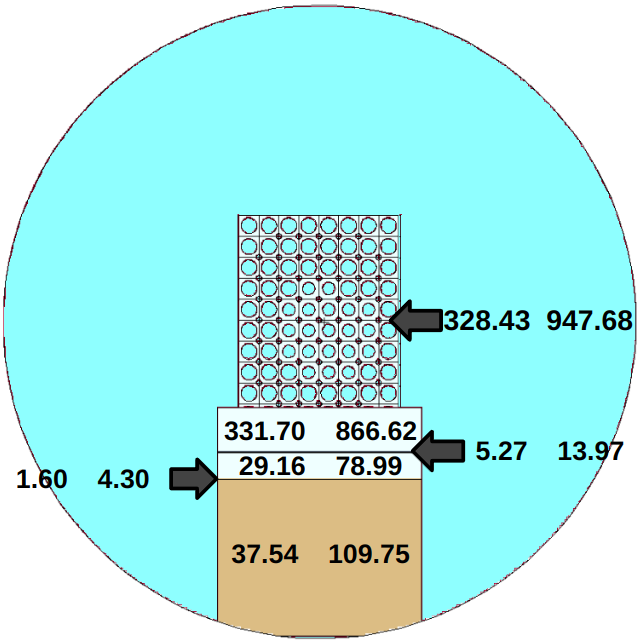
\includegraphics[width=0.75\linewidth]{figures/results_b}
    \hfill
    \caption{Delayed heating in the RA-6 reactor structures. Values expressed in $W$. Left: values corresponding to 1 MWth. Right: values corresponding to 3 MWth.}
    \label{fig:ra6-3}
\end{figure}

\begin{table}[htbp!]
  \centering
  \caption{Main results for delayed heating in the RA-6 reactor structures for operating powers of 1 and 3 MWth.}
  \label{tab:ra6-res}
  \begin{tabular}{cccc}
    \toprule
                    % & $H_{T, 1MW}/V [W/m^3]$  & $H_{T, 3MW}/V [W/m^3]$  & $ \frac{H_{T, 3MW}}{H_{T, 1MW}} - 1$  \\
                    & $H_{T, 1MW}/V [W/m^3]$  & $H_{T, 3MW}/V [W/m^3]$  & Rel. Diff. [\%]  \\
    \midrule
    Support grid    &  3291.14                &  9496.55                &  189 \%   \\
    BNCT 1st layer  &  3073.12                &  8029.02                &  161 \%   \\
    BNCT 2nd layer  &  5533.52                & 14668.54                &  165 \%   \\
    BNCT 3rd layer  &   459.27                &  1244.10                &  171 \%   \\
    BNCT 4th layer  &  1680.01                &  4515.01                &  169 \%   \\
    BNCT 5th layer  &   102.13                &  298.57                 &  192 \%   \\
    \bottomrule
  \end{tabular}
\end{table}


\section{Conclusions}

% Use conclusions from prelim and 8 and make specific to this thesis
% FROM 8-
% Intro
Safety analyses in research reactors require the estimation of heat deposited in experiments and reactor structures after reactor shutdown.
These analyses establish the heat-source term of those components, and the subsequent thermal-hydraulics calculations determine if an accident could jeopardize their integrity.
Additionally, detailed calculations help guide the optimization process of the design of irradiation targets.

In general, existing research reactor safety analyses have a strong focus on the reactor core and assume that the energy released after shutdown is deposited locally in the region of interest.
Moreover, many software packages rely on the same assumption, which may be inadequate in some cases.
On the other hand, an accurate assessment of the deposited energy across the reactor geometry allows for better determination of the heat removal requirements and ensures an effective cool down.
Instead of assuming locally deposited heat, this work utilizes detailed methods to target the specific reactor regions.

% Background
Chapter \ref{ch:lit} discussed various delayed heating calculation methods, and several publications relying on them.
The fact that the formal 3-step process accounts for the activation product decay and the time evolution after shutdown makes it better suited for this thesis than other methods.
Therefore, this chapter introduced a delayed heating calculation workflow based on the formal 3-step process that relies on MOAA.

% MOAA
MOAA is a Python package that couples MCNP and ORIGEN to streamline the calculation of the experiment source terms for experimental reactors.
This chapter described MOAA's workflow and the delayed heating calculation workflow and several practical aspects of the simulations.
The delayed heating calculation relies on MOAA for conducting the first two steps of the process, while the third step is conducted by multiple MCNP photon transport simulations.

% Results
Finally, this chapter demonstrated the delayed heating calculation capabilities by presenting four exercises.
The first exercise consisted of a code-to-code comparison between the workflow presented here and the Serpent Monte Carlo tool.
The purpose of this exercise was to understand the foundation of the method by comparing the results with Serpent.
The second exercise demonstrated the calculation workflow for a simple case geometry.
This exercise allows to better visualize the method and current capabilities.
The third and fourth exercises focus on full-size reactor exercises.
These exercises include the delayed heating in an ATR experiment and the RA-6 structures.
For the ATR experiment, the results showed the time evolution of the delayed heating up to 12 hours after shutdown, as well as the contribution to the heating from the different sources in the reactor.
For the RA-6 structures, the results displayed the delayed heating in several of the structural components and the comparison of the heating values for different power levels.

% Conclusions
As discussed in the results section, the calculation workflow can accommodate almost any MCNP input file, with some minimal modifications.
This workflow streamlines the calculation of delayed heating in research reactor experiments necessary for the development of experiment safety analysis.
Overall, this chapter presented delayed heating capabilities that rely on MOAA and that can be applied to any reactor.


\chapter{Shutdown Dose Rate}
\label{ch:sdr}

% Intro
While previous work utilized MOAA for delayed heating calculations \cite{fairhurst_decay_2022, fairhurst_demonstration_2022, fairhurst_database_2022}, a modification to the calculation workflow allows it to obtain the shutdown-dose rate.
The calculation workflow for the shutdown dose rate and delayed gamma heating is very similar, and they only change in how the deposition of energy manifests, either dose or heat.

% Motivation
The purpose of this chapter is to demonstrate the shutdown dose rate calculation workflow.
The development of experiment safety analysis also requires the determination of a \gls*{PIE} strategy, including the estimation of the dose rate in the surroundings of the experiments.
A capability like this allows to establish a \gls*{PIE} of an experiment from the dose rate standpoint, as well as design optimization.
% 
The equivalent dose rate from delayed gamma radiation is also an important factor for safely conducting work after reactor shutdown, such as periodic maintenance, fuel shuffling, among others \cite{ho_calculation_2022}.

Motivated by the calculation of shutdown dose rates in experiments, one experiment conducted at \gls*{ATR}, the \gls*{AGR1} \cite{sterbentz_agr1_2018}, requires special attention.
The \gls*{AGR1} was an experiment fueled with \gls*{TRISO} particles, which is a type of fuel form that is commonly found in \glspl*{HTGR}.
So, in order to properly model the AGR-1 experiment, it is insightful to understand the calculation workflow for shutdown dose rates in \glspl*{HTGR}.

% Shutdown dose rate in LWRs
Many publications have studied the shutdown dose rate in \glspl*{LWR}.
%
For example, Abrefah et al. \cite{abrefah_estimation_2018} estimated the dose rate of the spent fuel of the Ghana Research Reactor-1 (GHARR-1) to establish a proper unloading strategy for the \gls*{HEU} to \gls*{LEU} conversion of the reactor.
% The calculations used ORIGEN-S and MCNP6.
%
In another work, Ambrozic and Snoj \cite{ambrozic_JSIR2S_2020} studied the dose rate in the Jozef Stefan Institute (JSI) TRIGA reactor and validated their results against experimental measurements during normal operation and after shutdown.
% coupling MCNP6.2 and FISPACT-II
%
Bagheri et al. \cite{bagheri_gamma_2021} determined the dose rate from the spent fuel of the Tehran Research Reactor (TRR), validated their calculations against experimental measurements, and studied the photon emission rate of several isotopes for different fuel burnup values.
% Their calculations used ORIGEN2.1 and MCNPX2.7.

Although the shutdown dose rate associated with LWRs has been extensively studied, there are not many publicly available studies that focus on \glspl*{HTGR}.
%
For example, Suwoto et al. \cite{suwoto_neutron_2018} calculated the neutron dose rate in the working areas outside the \gls*{RPV} of the HTGR-10 reactor, concluding that the dose rates were compliant with the stipulated limits.
% MCNP5
% 
Ueta et al. \cite{ueta_shielding_2016} studied the shielding performance for the upper structure of the \gls*{HTTR} during normal operation.
Their study considered the active core, spent fuel, and equipment installed in the primary circuit as neutron and gamma radiation sources, and concluded that the neutron contribution to the dose was over 90\%.
% The spent fuel source was evaluated with ORIGEN2.
% 
Another study by Hamzah et al. \cite{hamzah_preliminary_2019} analyzed the dose rate distribution in the Reaktor Daya Eksperimental (RDE), a 10 MWth experimental pebble-bed reactor, during normal operation and after shutdown.
Their study estimated the dose rates in the working area and outside the RDE reactor building, concluding that the calculated values were below the stipulated limits.
% The latter relied on ORIGEN2 to determine the source strength of the decay gamma radiation.
%
% Conclusion
% Option 1
Ho et al. \cite{ho_calculation_2022} calculated the shutdown gamma distribution in the \gls*{HTTR}, relying on MCNP6 \cite{mcnp} and ORIGEN2 \cite{croff_origen2_1980} to obtain the gamma source distribution and MCNP6 to conduct the gamma transport at multiple cooling times.
Their work utilized the repeated structures from MCNP6 to model the decay sources from all the fuel rods explicitly, with the gamma radiation emitted from each rod with a uniform spatial distribution.
Most of the studies described above focus on the dose rates during normal operation or perform some level of homogenization to avoid the explicit modeling of the TRISO particles as decay radiation source.
% Option 2
% Up to this point, most of the studies described above focus mainly on the dose rates during normal operation or do not provide a thorough description of their methods for taking into account the decay gammas as a radiation source.
% % ho_calculation_2022
% In contrast, Ho et al. \cite{ho_calculation_2022} calculated the shutdown gamma distribution in the \gls*{HTTR} and provides a rigorous description of their implementation.
% Their calculations relied on MCNP6 \cite{mcnp} and ORIGEN2 \cite{croff_origen2_1980} to obtain the gamma source distribution and then their energy deposition was calculated using MCNP6 for different cooling times.
% Their work utilized the repeated structures from MCNP6 to model the sources from all the fuel rods explicitly with the gamma radiation emitted from each rod with a uniform spatial distribution.
% % Most of the studies focus mainly on the dose rates during normal operation or perform some sort of homogenization, neglecting the double heterogeneity of the fuel.

The objective of this work is to introduce a new shutdown dose rate calculation capability for TRISO-fueled experiments and HTGRs.
The modeling of HTGRs is challenging due to the fuel double heterogeneity, a distinctive characteristic in this type of reactor due to its fuel nature - i.e., the \gls*{TRISO} particles.
Previous work \cite{fairhurst_decay_2022, fairhurst_demonstration_2022, fairhurst_database_2022} utilized MOAA to calculate delayed heating by treating each depleted cell as an independent source of radiation.
However, one single HTGR core contains millions of TRISO particles, meaning that modeling each cell independently is not realistically possible.
This chapter of the thesis investigates the modeling of the AGR-1 experiment using the repeated structures from MCNP to explicitly model the TRISO particles as decay radiation source.

This chapter is organized as follows.
Section \ref{sec:methodology} details the main aspects of the calculation workflow.
Section \ref{sec:verif} introduces a verification exercise consisting of the delayed heating calculation of a simple geometry.
Section \ref{sec:agr} discusses an exercise studying the shutdown-dose rates of the \gls*{AGR1} experiment.
% \cite{fairhurst_sdr_2023}
Additionally, Section \ref{sec:micro} uses the workflow described here to study potential decommissioning strategies of a high-temperature gas-cooled microreactor.


\section{Methodology}
\label{sec:methodology}

% Intro: MOAA as the main solver
The calculations use the formal 3-step process to obtain the shutdown dose rates, consisting of the following three steps:
\begin{itemize}
  \item First, a neutron-transport simulation determines the neutron flux spatial and energy distribution during reactor operation.
  \item Second, an activation calculation estimates the energy distribution and emission probability of the decay photon sources after reactor shutdown.
  \item Third, a photon-transport simulation evaluates the dose rate.
\end{itemize}

% Workflow
As we can see, the calculation workflow for the shutdown dose rate and delayed gamma heating (Sec. \ref{sec:delheat}) is identical, and the only change is the evaluation of energy deposition resulting from the photon transport.
Overall, the calculation scheme, shown in Figure \ref{fig:workflow_4}, follows the formal 3-step process, in which MOAA conducts the first two steps, and an MCNP photon-transport simulation carries out the third step and estimates the dose rate with the following formula
% Photons deposit their energy globally thus requiring a transport simulation \cite{peterson-droogh_current_2018}.

% Formulas
% 1.6022 \times 10^{-19} \times 3600
\begin{align}
\dot{D}[Sv/h] &=  F4\!:\!p [pSv/src] \times \mathlarger{\sum}_i S_i \times 3.6 \times 10^{-9} \label{eq-dose} \\
S_i[\gamma/s] &= \int_{E} \varphi^\gamma_i(E) dE \\
s_i [-] &= S_i / \mathlarger{\sum}_j S_j
\end{align}
where $\dot{D}$ is the dose rate, $F4\!\!:\!\!p$ is the F4 tally for photons, $S_i$ is the total photon emission rate from region $i$, $\varphi^\gamma_i(E)$ is the photon source energy distribution from region $i$, and $s_i$ is the source emission probability of region $i$.
$F4\!\!:\!\!p$ result is expressed in $pSV$ per source particle by adding fluence-to-dose conversion factors \cite{icrp_116} to the MCNP input file.
The conversion factors consider an antero-posterior exposure to photons.

\begin{figure}[htbp!]
  \begin{center}
    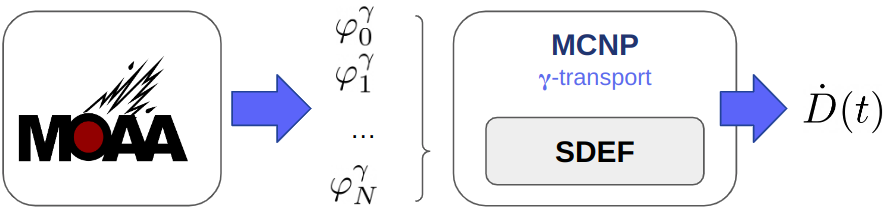
\includegraphics[width=0.85\linewidth]{figures/dose-flow}
  \end{center}
  \caption{Shutdown dose rate calculation scheme.}
  \label{fig:workflow_4}
\end{figure}


\section{Verification}
\label{sec:verif}

% Intro
This exercise consists of the delayed gamma heating calculation in a simple geometry.
The calculation workflow for the shutdown dose rate and delayed gamma heating is identical, and they only change in how the deposition of energy manifests, either dose or heat.
Three calculations were performed for this exercise.
The first calculation employs the explicit independent definition of each cell and provides the reference values.
The second calculation utilizes the repeated structures' approach.

The following equation calculates the delayed gamma heating
\begin{align}
H_{\gamma, Tr} [W] &= 1.6022 \times 10^{-13} \times \: ^* \! F8 [MeV] \times \mathlarger{\sum}_i S_i
\end{align}
where $H_{\gamma, Tr}$ is the energy deposited in the region of interest resulting from the photon transport, $^\ast F8$ is the energy deposition calculated by an $^\ast$F8 tally, and $S_i$ is the total photon emission rate from the region $i$ (see Eq. \ref{eq-ga-tr}).

% OLD RESULTS
% % Problem definition
% % Geometry
% The problem geometry is displayed in Figure \ref{fig:toy-geo2}.
% The core consists of a 4x4 array of fuel pins of 2.5 cm radius with an 8 cm pitch, and it is separated from the reflector tank by an inner shell of aluminum.
% The shell dimensions are an inner side length of 32 cm and a 2 cm thickness.
% The reflector tank is filled with light water, and its radius is 40 cm.
% The whole geometry has an 80 cm height.
% The fuel is 7.8\%-enriched uranium with a density of 10.5 g/cm$^3$, the inner shell is made of pure aluminum with a density of 2.7 g/cm$^3$, and the light water has a density of 1.0 g/cm$^3$.

% \begin{figure}[htbp!] %or H 
%     \centering
%     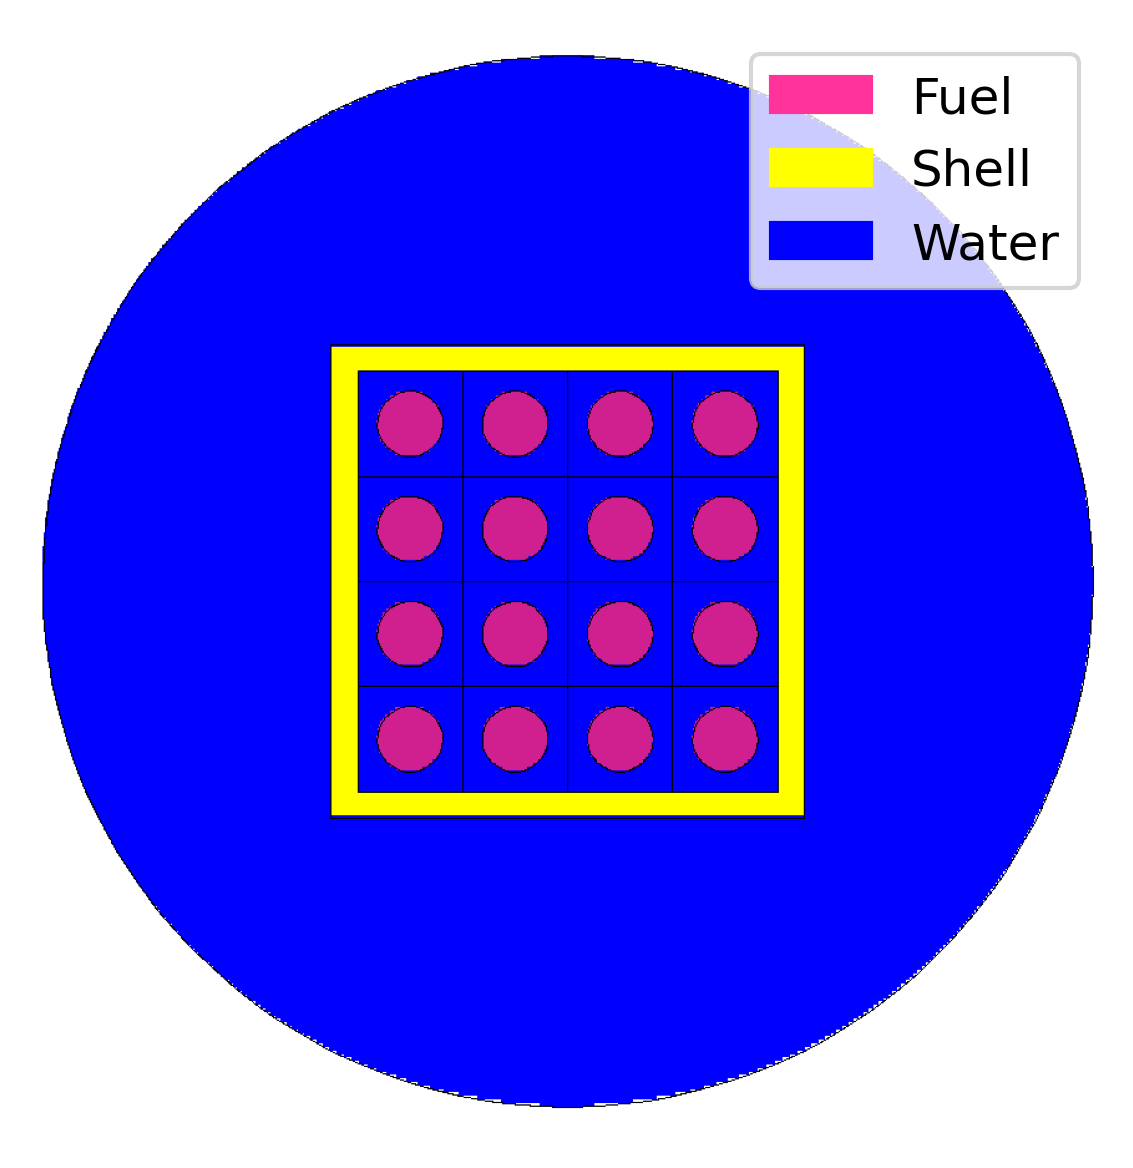
\includegraphics[width=0.60\linewidth]{figures/toy-problem.png}
%     \hfill
%     \caption{Verification problem geometry. The delayed gamma heating is calculated in the core inner shell.}
%     \label{fig:toy-geo2}
% \end{figure}

% % The Problem
% The main objective of the calculation is the estimation of the delayed gamma heating in the core inner shell, considering all the fuel pins as the radiation source.
% The delayed heating is calculated after a reactor operation at a 1 MW constant power for a 12-month cycle.

% % Results
% Table \ref{table:verif} summarizes the main results at the end of irradiation.
% While the heating equals 616.1 W in the reference case, the repeated structures' case predicts a heating of 685.2 W, which is 11.2\% larger than the reference value.
% To understand this result, we need to investigate other quantities in the results.
% The average neutron flux and total photon intensity show a relative difference smaller than 0.1\%.
% Figure \ref{fig:ver-comp} displays the uranium composition evolution during irradiation.
% The uranium evolution displays a relative difference smaller than 0.1\%.

% \begin{table}[!htb]
%   \centering
%   \caption{End of irradiation integral results.}
%   \label{table:verif} 
%   \begin{tabular}{l|cc|c}
%   \toprule
%           & Reference & Rep. Struct. & Rel. Diff. [\%] \\ % (RS/REF - 1)*100
%   \midrule
%    Delayed gamma heating [W]           &  616.1  &  685.2  & 11.2 \\
%    Ave. neutron flux [10$^{13}$ n/cm2/s] &  2.377  &  2.375  & 0.08 \\
%    Tot. photon intensity [10$^{17}$ $\gamma$/s] &  3.672  &  3.672  & 0.01 \\
%   \bottomrule
%   \end{tabular}
% \end{table}

% \begin{figure}[htbp!] %or H 
%     \centering
%     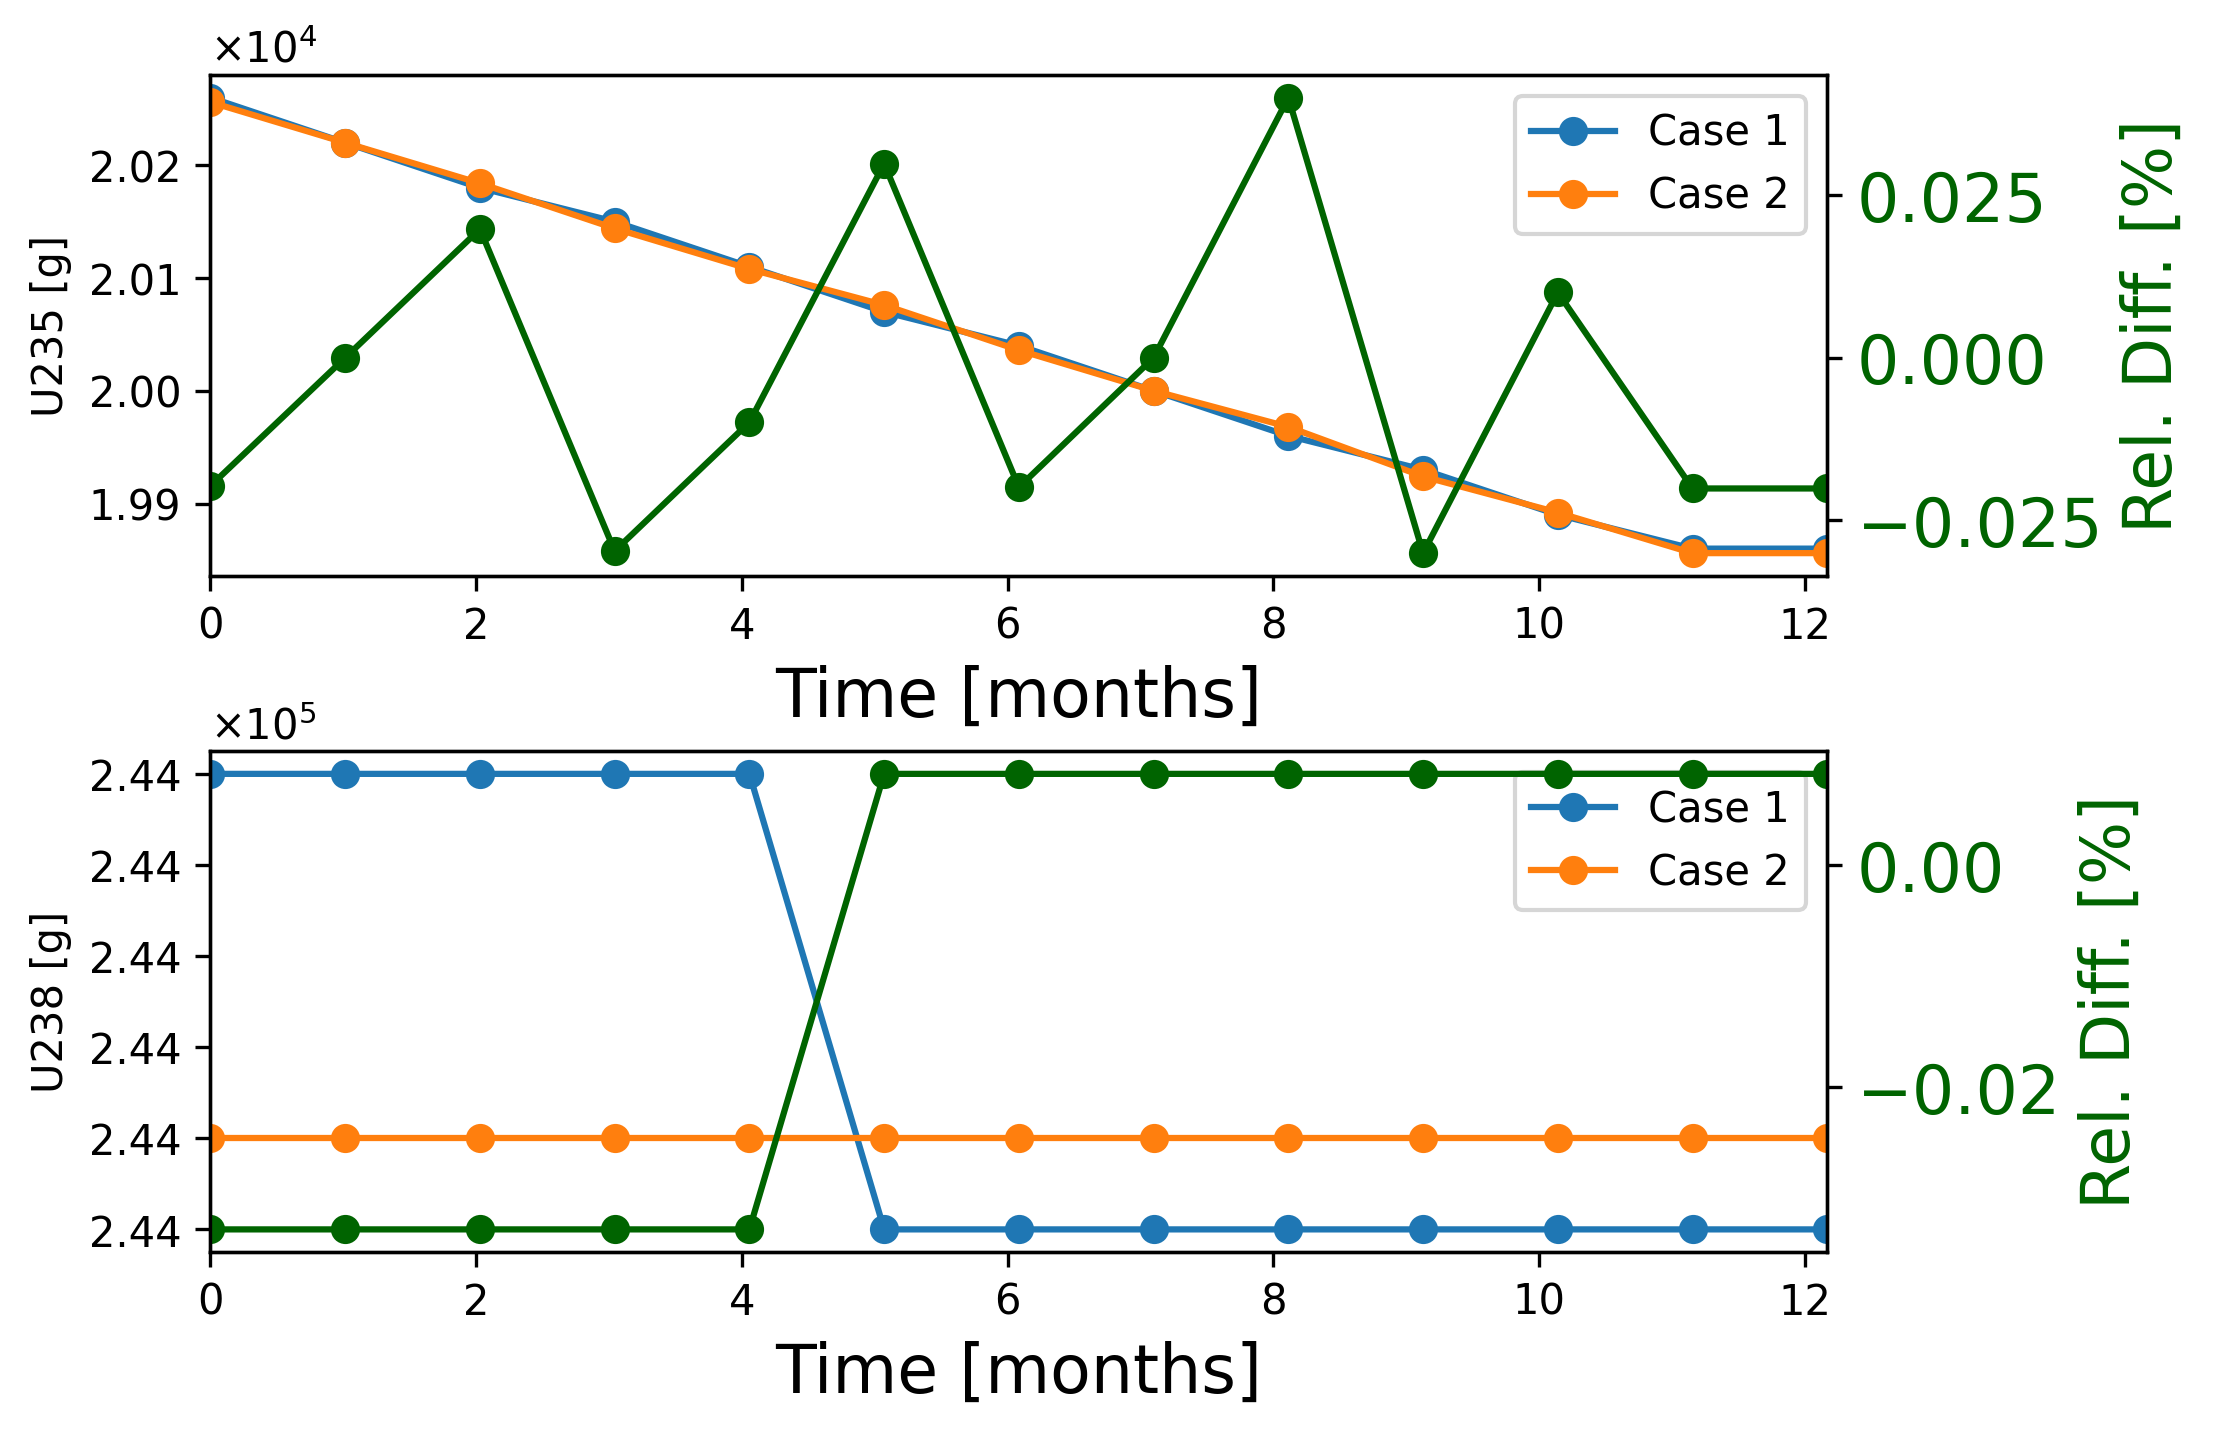
\includegraphics[width=0.98\linewidth]{figures/composition-time}
%     \hfill
%     \caption{Comparison of the uranium mass during reactor operation.}
%     \label{fig:ver-comp}
% \end{figure}

% % gamma intensity
% Figure \ref{fig:gamma-sources} displays a comparison between the repeated structures and the reference cases of the gamma source intensities in the fuel pins.
% The sources in the repeated structures' case have a uniform value across the geometry.
% The definition of the repeated structures requires the utilization of universes, and all the cells defined by the same universe are subject to the same flux level, an average value, and hence their depletion is uniform.
% The sources in the reference case are strongest in the center of the core and decrease towards the periphery, due to the flux shape, which is strongest in the center.
% Finally, given that in the repeated structures' case, the gamma source intensities are stronger in the periphery than in the reference case, and these pins contribute the most to the heating due to their proximity, the delayed heating in the core inner shell is higher.

% \begin{figure}[htbp!] %or H 
%     \centering
%     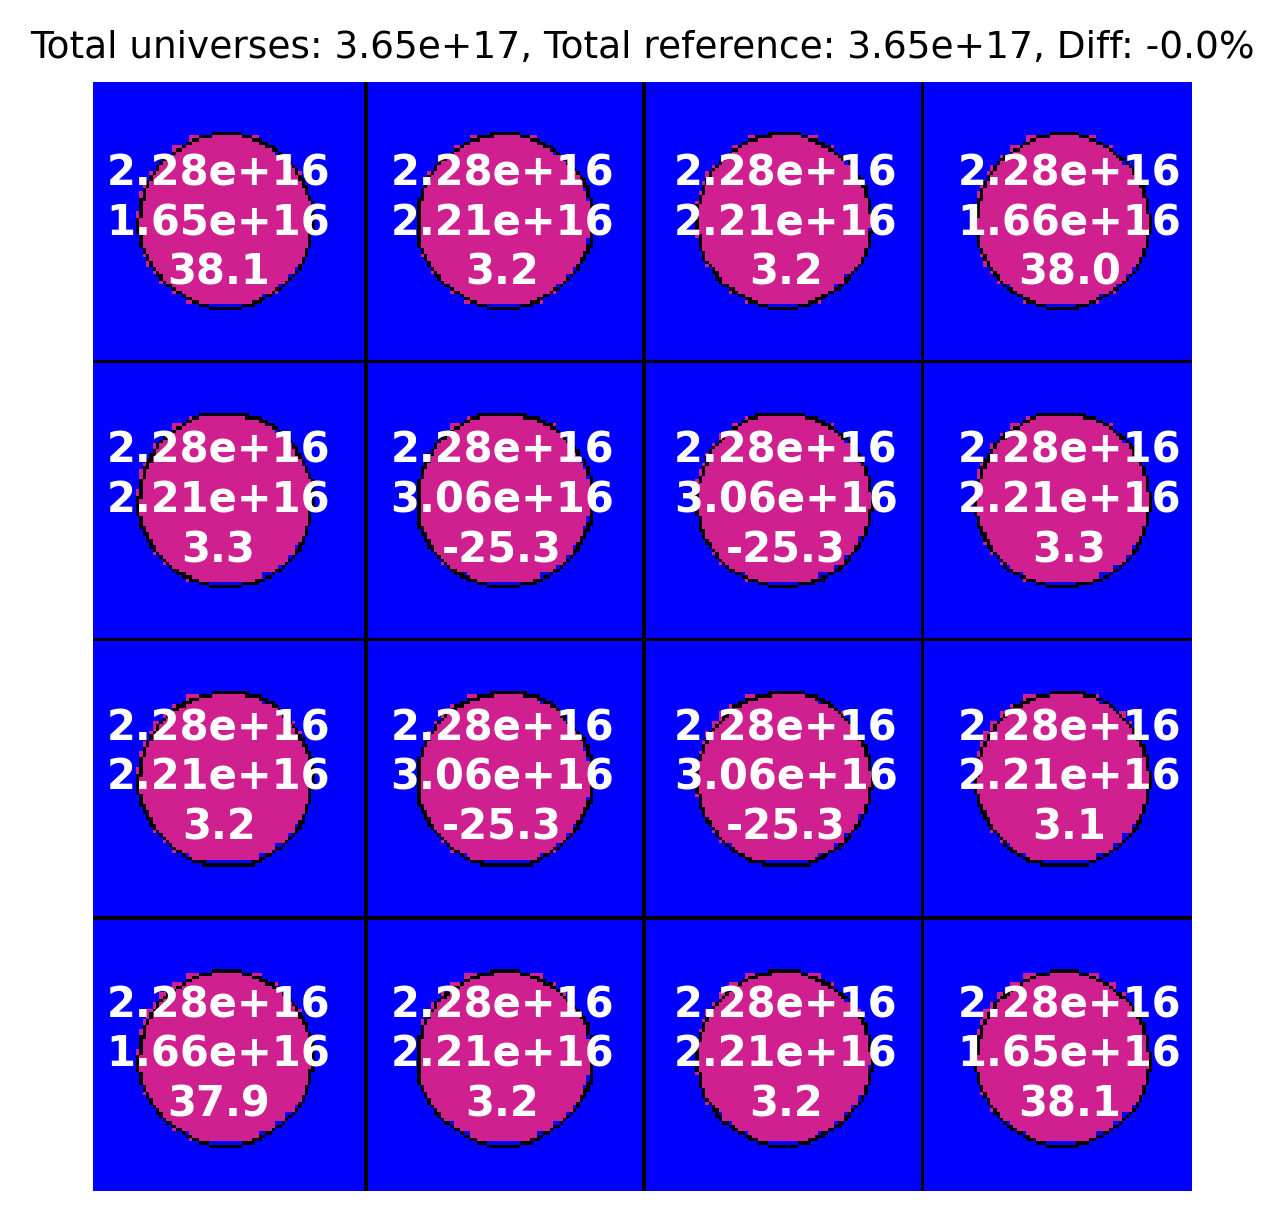
\includegraphics[width=0.80\linewidth]{figures/moaa-ref-uni-gamma-intens}
%     \hfill
%     \caption{Comparison of the intensity of the gamma sources in the fuel pins. Top value corresponds to the input file defined with repeated structures. Intermediate value corresponds to the reference intensities. Intensities expressed in decays per second. Lower value corresponds to the relative difference in \%.}
%     \label{fig:gamma-sources}
% \end{figure}

% % Conclusions from 13-
% This exercise studied the delayed heating calculation in repeated structures, such as the ones that are necessary to define HTGR models.
% Taking advantage of the MCNP input definition using repeated structures allows for simplifying the definition of cells contributing to the delayed heating/shutdown dose rates.
% Even though the results for the repeated structures' case show an overestimation of the delayed heating, the approach seems to yield a reasonable approximation.
% The results and conclusions drawn from this exercise set the path forward for the next exercises, which use the same approach for calculating the shutdown dose rate in HTGRs.

% Problem definition
% Geometry
The problem geometry is displayed in Figure \ref{fig:toy-geo2}.
The core consists of an 8x8 array of fuel pins of 1.25 cm radius with a 4 cm pitch, and it is separated from the reflector tank by an inner shell of aluminum.
The shell dimensions are an inner side length of 32 cm and 2 cm thickness.
The reflector tank is filled with light water, and its radius is 40 cm.
The whole geometry is 80 cm high.
The fuel is 7.8\%-enriched uranium with a density of 10.5 g/cm$^3$, the inner shell is made of pure aluminum with a density of 2.7 g/cm$^3$, and the water has a density of 1.0 g/cm$^3$.

\begin{figure}[htbp!] %or H 
    \centering
    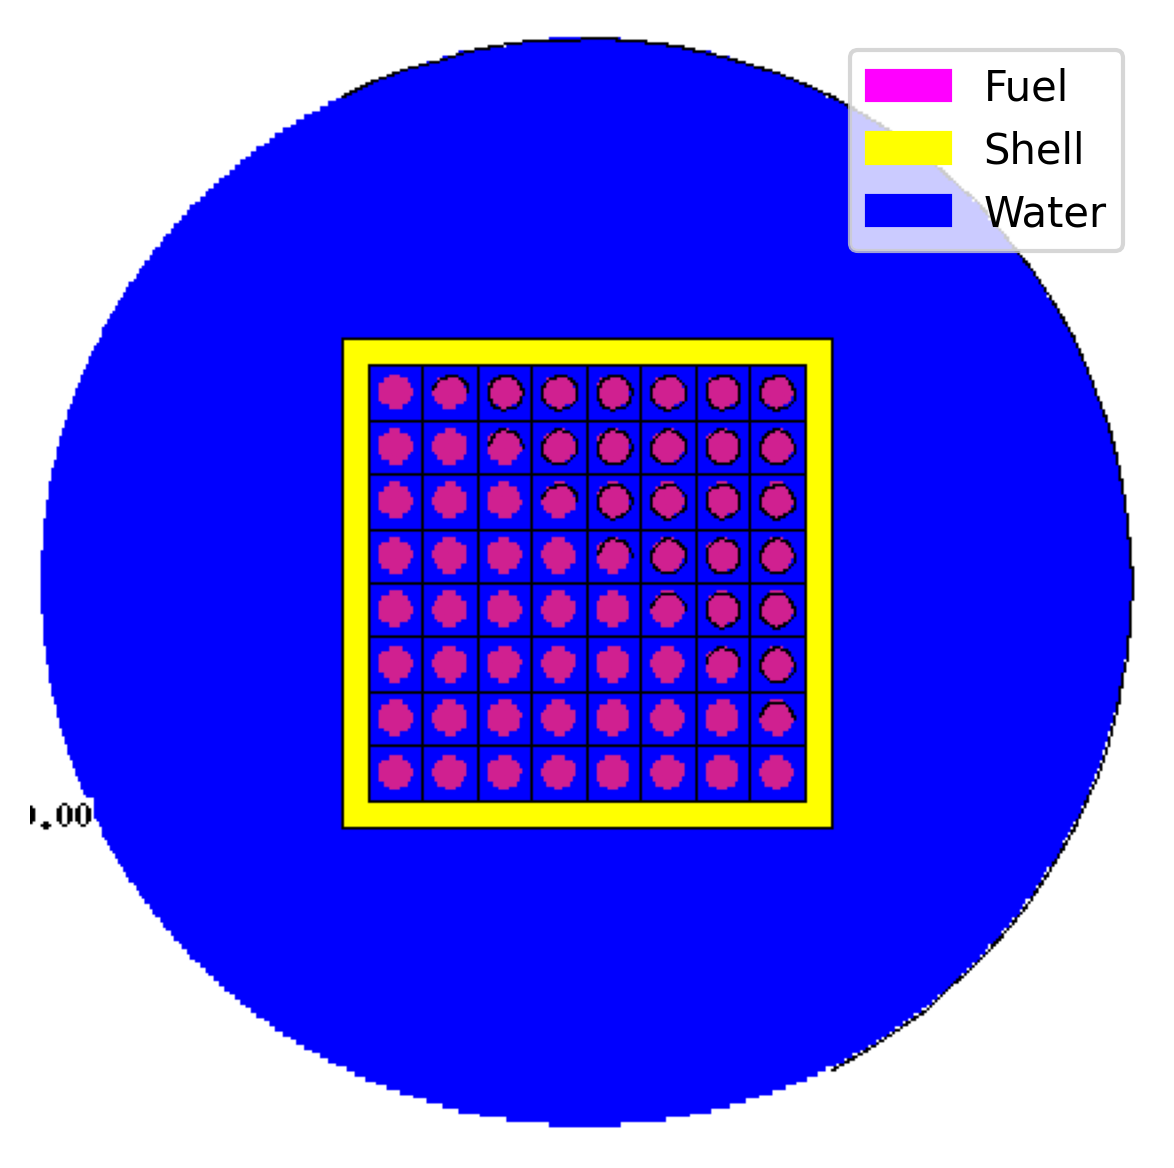
\includegraphics[width=0.6\linewidth]{figures/toy-problem-b.png}
    \hfill
    \caption{Verification problem geometry. The delayed gamma heating is calculated in the core inner shell.}
    \label{fig:toy-geo2}
\end{figure}

% The Problem
The main objective of the calculation is the estimation of the delayed gamma heating in the core inner shell, considering all the fuel pins as the radiation source.
The delayed heating is calculated after a reactor operation at a 1 MW constant power for a 12-month cycle.

% Results
Table \ref{table:verif} summarizes the main results at the end of irradiation.
While the heating equals 675.0 W in the reference case, the repeated structures' case predicts a heating of 780.4 W, which is 15.6\% larger than the reference value.
To understand this result, we need to investigate other quantities.
The average neutron flux and total photon intensity show a relative difference smaller than 0.1\%.
Figure \ref{fig:ver-comp} displays the uranium composition evolution during irradiation.
The uranium evolution displays a relative difference smaller than 0.1\%.

\begin{table}[!htb]
  \centering
  \caption{Comparison of end of irradiation integral results for the reference and repeated structure approaches.}
  \label{table:verif}
  \begin{tabular}{l|cc|c}
  \toprule
                                           & Reference  & Rep. Struct. & Rel. Diff. [\%] \\ % (RS/REF - 1)*100
  \midrule
   Delayed gamma heating [W]               & 675.0      & 780.4        & 15.6 \\
   Ave. neutron flux [10$^{13}$ n/cm2/s]   & 1.868      & 1.867        & 0.07 \\
   Tot. photon intensity [10$^{17}$ $\gamma$/s] &  3.666  &  3.668     & 0.04 \\
  \bottomrule
  \end{tabular}
\end{table}

\begin{figure}[htbp!] %or H 
    \centering
    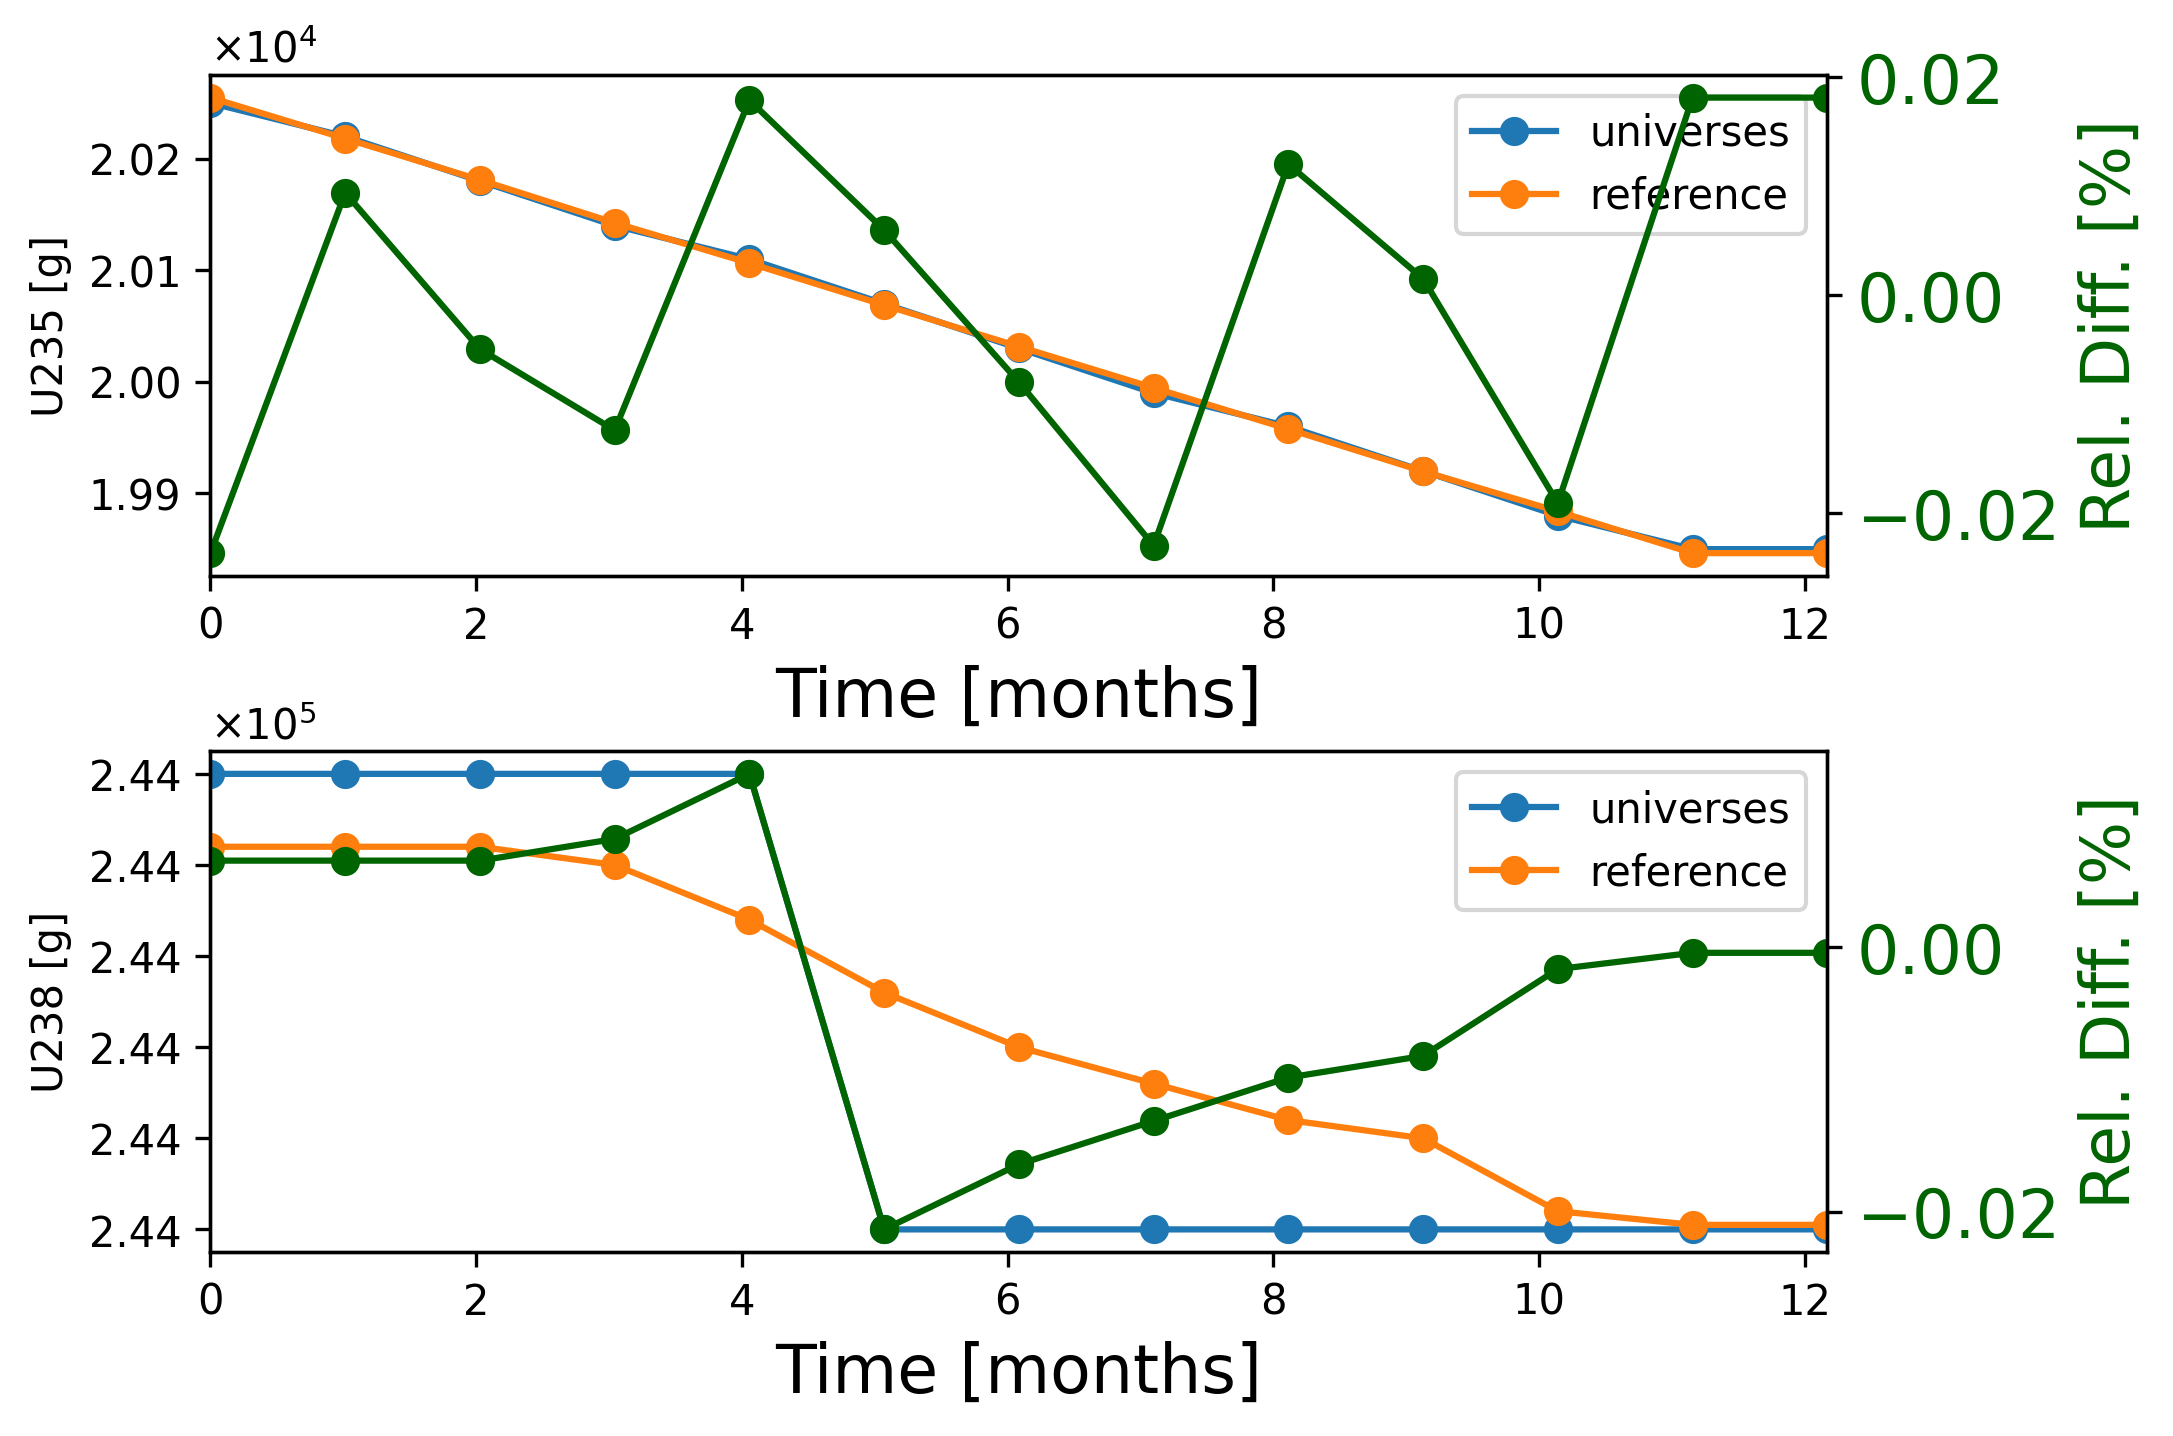
\includegraphics[width=0.65\linewidth]{figures/moaa-ref-uni-composition-time-b}
    \hfill
    \caption{Comparison of the uranium mass during reactor operation.}
    \label{fig:ver-comp}
\end{figure}

% gamma intensity
Figure \ref{fig:gamma-sources} displays a comparison between the repeated structures and the reference cases of the gamma source intensities in the fuel pins.
The sources in the repeated structures' case have a uniform value across the geometry.
The definition of the repeated structures requires the utilization of universes, and all the cells defined by the same universe are subject to the same flux level, an average value, and hence their depletion is uniform.
The sources in the reference case are strongest in the center of the core and decrease towards the periphery, due to the flux shape, which is strongest in the center.
Finally, the gamma source intensities in the repeated structures' case are stronger in the periphery than in the reference case.
As these pins contribute the most to the heating of the shell due to their proximity, the delayed heating in the core inner shell is higher.

\begin{figure}[htbp!] %or H 
    \centering
    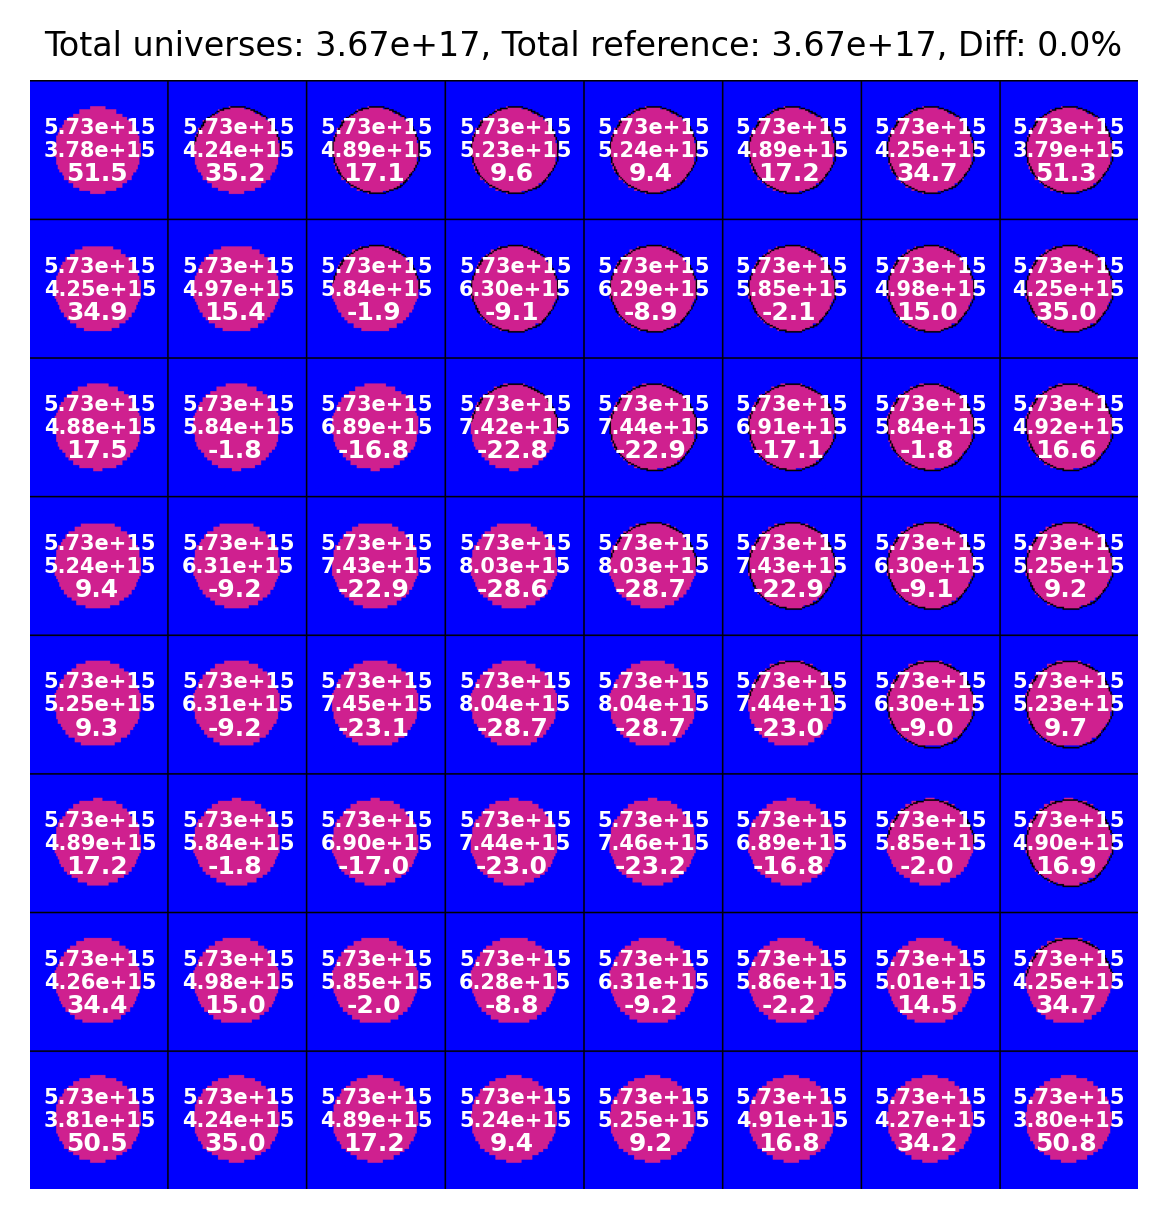
\includegraphics[width=0.65\linewidth]{figures/moaa-ref-uni-gamma-intens-b}
    \hfill
    \caption{Comparison of the intensity of the gamma sources in the fuel pins. The top value corresponds to the repeated structure approach. The intermediate value corresponds to the reference values. Intensities expressed in decays per second. The lower value corresponds to the relative difference in \%.}
    \label{fig:gamma-sources}
\end{figure}

As shown in Figure \ref{fig:gamma-sources}, the accuracy of the repeated structure approach is affected when the problem shows a strong spatial effect.
This suggests that using a repeated structure that comprehends the whole core is not the right approach.
Instead, a better approach would consider the flux shape variation to choose the repeated structures.
This exercise was also conducted using repeated structures but arranging the fuel pins in groups of 4.
Table \ref{table:verif2} displays the results for that case.
The relative difference for the delayed gamma heating is 4.3\%, while the rest of the results do not change considerably.
The results show that grouping the structures based on the location, and hence similar flux levels, yields better results.

\begin{table}[!htb]
  \centering
  \caption{Comparison of end of irradiation integral results for the reference and repeated structure approaches.}
  \label{table:verif2}
  \begin{tabular}{l|cc|c}
  \toprule
                                           & Reference  & Rep. Struct. & Rel. Diff. [\%] \\ % (RS/REF - 1)*100
  \midrule
   Delayed gamma heating [W]               & 675.0       & 704.3       &  4.3  \\
   Ave. neutron flux [10$^{13}$ n/cm2/s]   & 1.868       & 1.867       & -0.03 \\
   Tot. photon intensity [10$^{17}$ $\gamma$/s] &  3.666 & 3.667       &  0.03 \\
  \bottomrule
  \end{tabular}
\end{table}

% Conclusions from 13-
This exercise studied the delayed heating calculation in repeated structures, such as the ones that are necessary to define HTGR models.
Taking advantage of the MCNP input definition using repeated structures allows for simplifying the definition of cells contributing to the delayed heating/shutdown dose rates.
Even though the results for the repeated structures' case show an overestimation of the delayed heating, the approach yields a reasonable approximation when considering the flux spatial variation.
The results and conclusions drawn from this exercise set the path forward for the next exercises, which use the same approach for calculating the shutdown dose rate in HTGRs.


\section{AGR-1}
\label{sec:agr}

% Depletion results: AGR1 benchmark

% AGR-1
The \gls*{AGR1} \cite{sterbentz_agr1_2018} was a TRISO-particle irradiation test in the \gls*{ATR}, a 250-MWth high flux test reactor located at the Reactor Technology Complex of the \gls*{INL}.
This experiment was part of the \gls*{DOE} Advanced Gas Reactor Fuel Development and Qualification Program to support the \gls*{NGNP} program.

% ATR: reactor description
Figure \ref{fig:atrq} shows the MCNP quarter model of ATR, which represents the core east quadrant, which is used for the simulations.
This model simplifies the reactor geometry by grouping the fuel plates into three radial zones.
% AGR-1 in ATR
The AGR-1 experiment was placed in the B-10 position and irradiated over 13 power cycles for a period corresponding to three years.

% ATR figure of the model
\begin{figure}[htbp!] %or H 
    \centering
    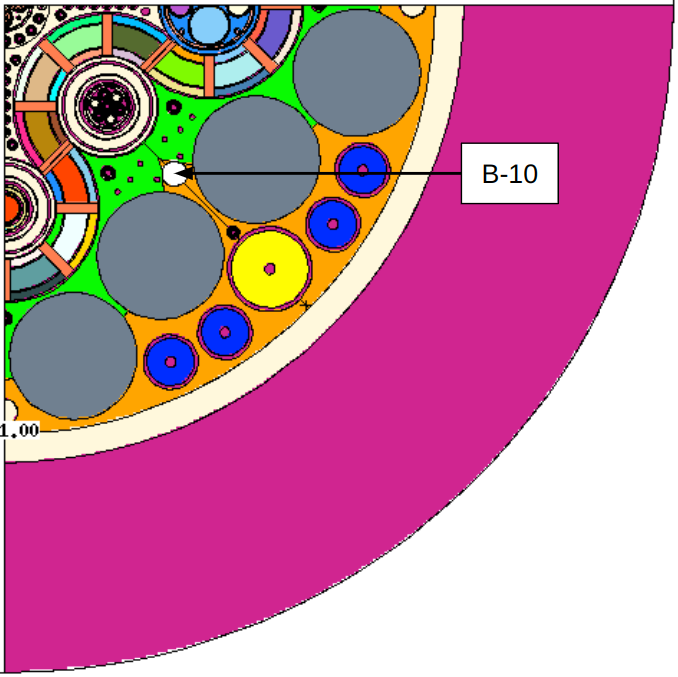
\includegraphics[width=0.70\linewidth]{figures/atr-quarter2}
    \hfill
    \caption{MCNP quarter model of ATR.}
    \label{fig:atrq}
\end{figure}

% Benchmark
The AGR-1 Depletion Benchmark \cite{sterbentz_agr1_2018} describes the experiment test train, shown in Figure \ref{fig:agr-geo}.
The test train consists of six cylindrical capsules vertically stacked, wherein the compacts are separated into three columns, with each column containing four compacts, adding up to a total of 72 compacts.
The experiment includes four different types of compact.
Capsules 3 and 6 contain the baseline compact, capsule 5 contains variant 1, capsule 2 contains variant 2, and capsules 1 and 4 contain variant 3.
The difference between compact types is that the particle layers change slightly in thickness and density, while the fuel kernel remains the same.
Additionally, each type of compact has a different number of embedded particles.
The main model simplifications are that the hafnium (Hf) shroud surrounds the whole circumference of the capsule, the gas lines, thermocouples, and thru-tubes are neglected, and the TRISO particles are arranged in a regular lattice.

\begin{figure}[htbp!] %or H
  \centering
  \begin{subfigure}{0.49\textwidth}
    \centering
    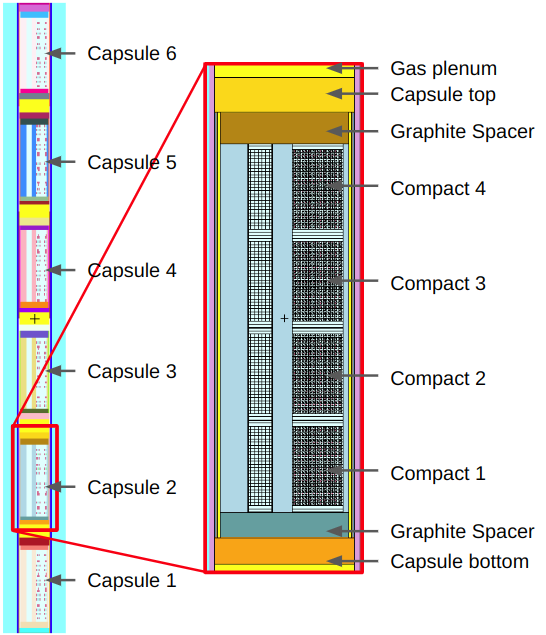
\includegraphics[width=0.9\linewidth]{figures/agr-paper-1}
    \caption{Axial view.}
    \label{fig:agr-a}
  \end{subfigure}
  \begin{subfigure}{0.49\textwidth}
    \centering
    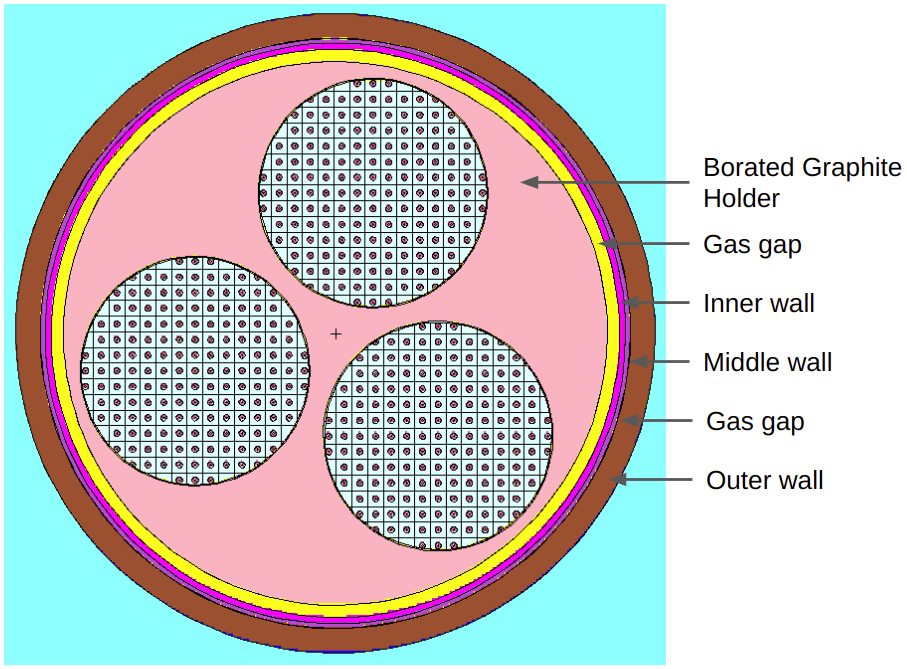
\includegraphics[width=0.9\linewidth]{figures/agr-paper-2}
    \caption{Top view.}
    \label{fig:agr-b}
  \end{subfigure}
  \caption[benchmark]{AGR-1 experiment geometry.}
  \label{fig:agr-geo}
\end{figure}

% \begin{figure}[htbp!] %or H 
%     \centering
%     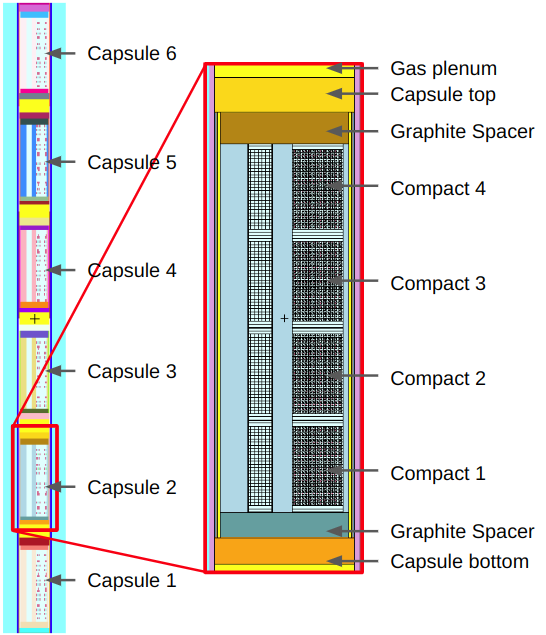
\includegraphics[width=0.90\linewidth]{figures/agr-paper-1}
%     \hfill
%     \caption{Axial view of the AGR-1 experiment.}
%     \label{fig:agr-1}
% \end{figure}

% \begin{figure}[htbp!] %or H 
%     \centering
%     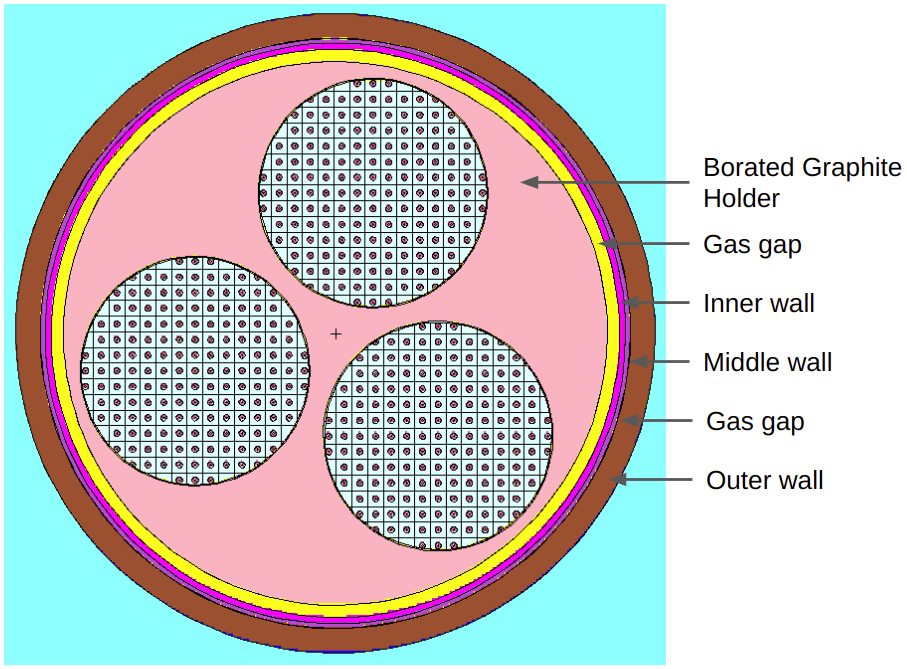
\includegraphics[width=0.90\linewidth]{figures/agr-paper-2}
%     \hfill
%     \caption{Top view of the AGR-1 experiment.}
%     \label{fig:agr-2}
% \end{figure}

The benchmark data includes for each time step: the lobe power, the OSCC positions, and the neck shim insertion condition.
Figure \ref{fig:agr-data} shows the benchmark data for the first irradiation cycle or cycle 138B.
Because the data includes 662 time steps, and to reduce the complexity of the model, this work considers the power, OSCC position, and neck shim insertion condition to take the cycle average value.
For the neck shim insertion, the average value is considered the cycle predominant insertion condition.
For example, if the NE 1 rod is inserted through most of the cycle, this work assumes that it is inserted throughout the whole cycle length.
For tally normalization, the B-10 position tally data is typically normalized to an east lobe power defined as the average of the northeast, center, and southeast lobe powers.
For the fuel composition, the MCNP model defines the driver fuel for the \gls*{BOC} 145A and assumes it to be appropriate for the \gls*{BOC} of all the cycles.
This work takes that assumption one step further and considers the driver fuel composition to remain constant during all the simulations.

\begin{figure}[htbp!] %or H
  \centering
  \begin{subfigure}{1\textwidth}
    \centering
    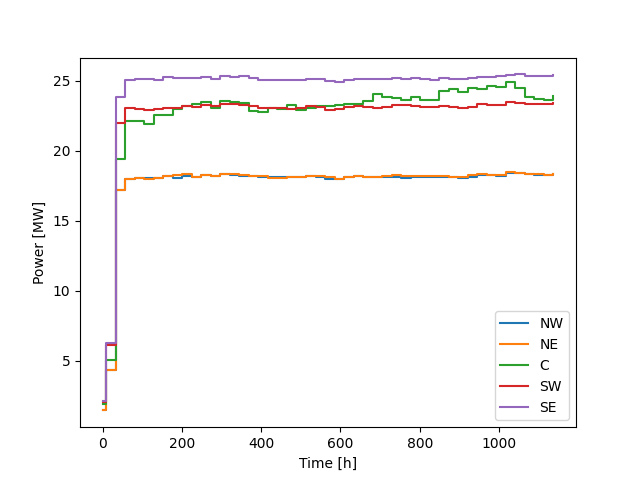
\includegraphics[width=0.55\linewidth]{figures/power_cycle_138B}
    \caption{Lobe power.}
    \label{fig:agrd-a}
  \end{subfigure}
  \begin{subfigure}{1\textwidth}
    \centering
    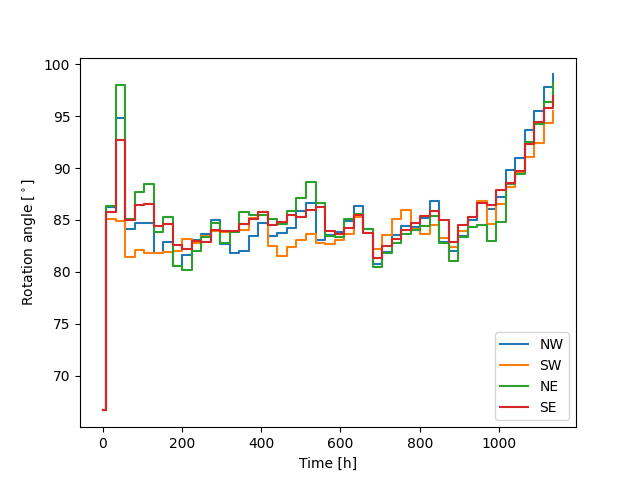
\includegraphics[width=0.55\linewidth]{figures/oscc_cycle_138B}
    \caption{OSCC rotation angle.}
    \label{fig:agrd-b}
  \end{subfigure}
  \begin{subfigure}{1\textwidth}
    \centering
    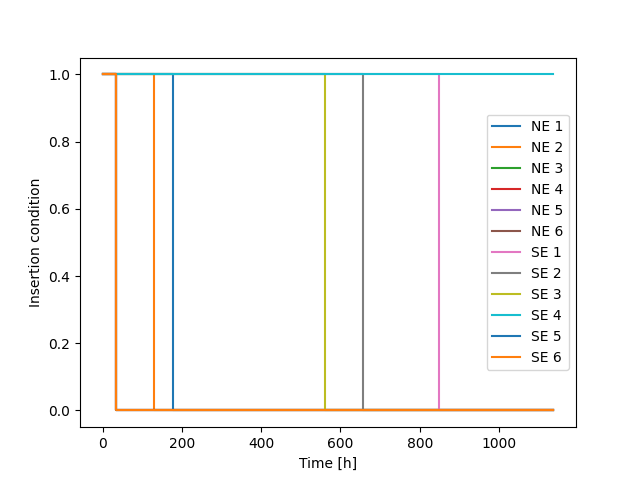
\includegraphics[width=0.55\linewidth]{figures/neck_cycle_138B}
    \caption{Neck shim insertion condition, where $0/1$ means withdrawn/inserted.}
    \label{fig:agrd-c}
  \end{subfigure}
  \caption[benchmark]{AGR-1 benchmark data for first irradiation cycle (cycle 138B).}
  \label{fig:agr-data}
\end{figure}


% Results
Figure \ref{fig:agr-deplet} displays the experiment burnup as a function of the axial position.
This figure compares this work's results versus the benchmark results.
As the raw data from benchmark results are not available, this figure shows both results overlapped, allowing for the visualization of the following phenomena.
The benchmark results include more data points than this work.
While the benchmark subdivides each capsule into eight pieces, this work considers only one average value.
Stacks 1 and 2 show the largest burnup values, as they are the closest to the reactor center.
This work results agree on this aspect with the benchmark results.
The burnup shape for each capsule displays higher values in the bottom and top ends.
The reason for this is the presence of the graphite spacers in the bottom and top regions of each capsule.
This result is also consistent with the benchmark results.
Finally, this work predicts a lower burnup than the benchmark results.
The reason for this is the modeling simplification of considering the average values for each cycle, and most importantly, utilizing the cycle average power.
Although not shown here, some cycles include a reactor shutdown, in which the reactor total power becomes zero (even for 40 days).
For these cycles, the average cycle values simplification is expected to underpredict the cycle burnup.
For future reference, this simplification should not be used when trying to follow the benchmark formally.
However, for the purpose of this work focusing on shutdown dose rates, this simplification and consistent results are deemed valid. 

\begin{figure}[htbp!] %or H 
    \centering
    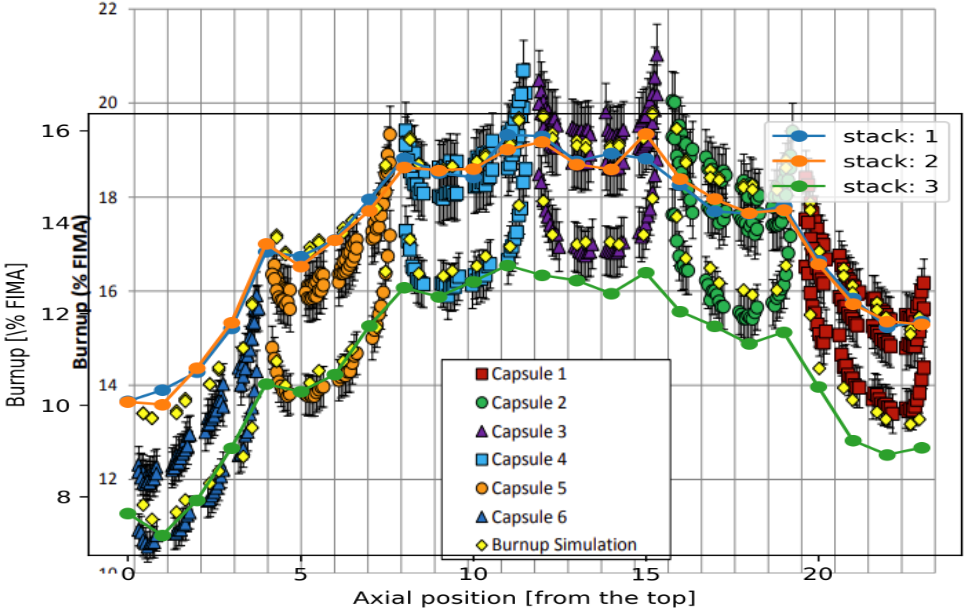
\includegraphics[width=0.9\linewidth]{figures/agr-depletion}
    \hfill
    \caption{AGR-1 experiment burnup as a function of the axial position.}
    \label{fig:agr-deplet}
\end{figure}

Table \ref{table:agr-contr} shows the contribution from all the photon sources at different decay times.
The graphite spacers and holders have the smallest contribution.
The holders contain boron and hence have a higher contribution than the spacers.
After one day, the largest contribution comes from fuel at 53.19\% followed by the Hf shroud with a contribution of 41.64\%.
After 30 days, the contribution from the fuel decreases to 30.03\% while the Hf shroud contribution of 62.11\% becomes predominant.
After 365 days, the Hf shroud contribution drops, and the largest contributor becomes the fuel at 56.95\%, followed by the structures of stainless steel which add up to 42.54\%. 
The total source intensities decrease two orders of magnitude after a 365-day decay.

\begin{table}[!htb]
  \centering
  \caption{Photon source contribution by decay time.}
  \label{table:agr-contr} 
  \begin{tabular}{lcccc}
  \toprule
  Contribution                 & Units  & 1 day        & 30 days        & 365 days      \\
  \midrule
  Fuel                         & \%     & 53.19         & 30.03          & 56.95         \\
  Bottom support SS316L        & \%     & 0.76          & 1.17           & 6.47          \\
  Inner wall SS316L            & \%     & 0.43          & 0.63           & 3.07          \\
  Top support SS316L           & \%     & 0.85          & 1.3            & 7.10          \\
  Outer wall SS316L            & \%     & 3.13          & 4.77           & 25.9          \\
  Low graphite spacer          & \%     & 6.93$\times$10$^{-10}$  & 2.56$\times$10$^{-9}$  & 6.37$\times$10$^{-8}$  \\
  Upper graphite spacer        & \%     & 8.04$\times$10$^{-10}$  & 2.96$\times$10$^{-9}$  & 7.38$\times$10$^{-8}$  \\
  Borated graphite holder      & \%     & 7.59$\times$10$^{-7}$   & 2.77$\times$10$^{-6}$  & 6.14$\times$10$^{-5}$  \\
  Hf shroud                    & \%     & 41.64         & 62.11          & 0.50          \\ \hline
  Total                        & $\gamma$/s  & 1.199$\times$10$^{15}$  & 3.2529$\times$10$^{14}$  & 1.305$\times$10$^{13}$  \\
  \bottomrule
\end{tabular}
\end{table}

% Figure \ref{fig:agr-dose} displays the dose rate surrounding the AGR test train during the \gls*{PIE}.
% The dose rate is calculated for the experiment located in a 1x1 m box at different decay times.
% % shape:
% The dose rate is plotted over the red line shown in the 2D plot, and as expected it has a $1/r^2$ shape.
% The highest value is in the proximity of the experiment for all the decay times.
% % max values over time
% After one day, the highest value is greater than 600 Sv/h, and it decreases to 30 Sv/h at 1 m from the experiment.
% After 30 days, the values are reduced about four times, and the highest value is slightly greater than 175 Sv/h, and it decreases to 5 Sv/h at 1 m from the experiment.
% After 365 days, the values are reduced about 200 times, and the highest value is slightly greater than 3.5 Sv/h, and it decreases to 0.2 Sv/h at 1 m from the experiment.

% \begin{figure}[htbp!] %or H
%   \centering
%   \begin{subfigure}{.9\textwidth}
%     \centering
%     \includegraphics[width=1\linewidth]{dose_1}
%     \caption{}
%   \end{subfigure}
%   \begin{subfigure}{.9\textwidth}
%     \centering
%     \includegraphics[width=1\linewidth]{dose_30}
%     \caption{}
%   \end{subfigure}
%   \begin{subfigure}{.9\textwidth}
%     \centering
%     \includegraphics[width=1\linewidth]{dose_365}
%     \caption{}
%   \end{subfigure}
%   \caption[Three solutions]{Dose rate for the PIE of AGR in a 1x1 m room and the values over the line denoted in red. Dose rates for different decay times: (a) 1 day, (b) 30 days, (c) 365 days.}
%   \label{fig:agr-dose}
% \end{figure}

Table \ref{table:agr-dose} shows the dose rate at different distances from the center of the AGR test train by decay time.
% Discussion
The results show that even after one year decay, and at 98 cm distance from the experiment, the exposure from the experiment decay is high.
For that reason, the experiment \gls*{PIE} would need to await more than 1 year to be conducted or utilize a hot cell with the appropriate shielding to prevent any unnecessary exposure of the personnel.

\begin{table}[!htb]
  \centering
  \caption{Dose rate at different distances from the center of the experiment by decay time. Values expressed in Sv/h.}
  \label{table:agr-dose} 
  \begin{tabular}{lcccc}
  \toprule
  Distance   & 1 day        & 30 days        & 365 days      \\
  \midrule
  6 cm       & 666.2         & 190.3          & 3.7           \\
  46 cm      & 72.7          & 20.4           & 0.4           \\
  98 cm      & 25.4          & 7.3            & 0.1           \\
  \bottomrule
\end{tabular}
\end{table}


\section{The $\mu$HTGR}
\label{sec:micro}


% Intro to HTGRs
% Motivation - from 12-
\Glspl*{HTGR} have gained a lot of attention in the past few decades.
% VHTR 
In 2002, the \gls*{VHTR} was proposed as one of the Generation-IV nuclear energy systems for the co-generation of electricity and hydrogen \cite{doe_vhtr_2002}.
% NGNP
In 2006, the \gls*{DOE} and the \gls*{INL} established the \gls*{NGNP} project to develop, license, build, and operate a prototype modular \gls*{HTGR} to produce hydrogen while generating electric power \cite{ngnp}.
% Add more examples of HTGRs built/developed in the past couple of decades, maybe another micro-reactor ?
More recent examples of HTGRs are new microreactor designs.
% StarCore
StarCore Nuclear has partnered with the local government of Pinawa, Canada to demonstrate the powering of off-grid communities and mining companies with an HTGR \cite{starcore}.
% BWXT
The \gls*{DOD} has recently awarded a contract to BWXT to deliver a transportable 1-5 MWe HTGR to be completed and delivered by 2024 \cite{bwxt}.
% USNC
The \gls*{UIUC} has partnered with the \gls*{USNC} to build a microreactor on its campus, a 10 MWth \gls*{HTGR} \cite{uiuc-mmr2}.
The new reactor facility will offer UIUC a diverse set of opportunities for research, including instrumentation and control, multi-physics validation, reactor prototype testing, and micro-grid operations.

HTGR technology presents many distinct features from the current \gls*{LWR} fleet, and potential decommissioning strategies should take them into consideration.
After reactor shutdown, the ongoing decay may inflict dose on workers and equipment in the reactor surroundings.
In \glspl*{LWR}, the common strategy entails flooding the entire reactor cavity to remove the spent fuel, as the water column between the assemblies and the operators provides enough shielding.
% High-temperature graphite oxidation
HTGRs cannot, however, implement such a strategy because of the presence of large volumes of high-temperature graphite in the core, and this could lead to graphite oxidation \cite{oxidation}, degrading its structural and functional properties.
Nevertheless, the proper characterization of the shutdown dose rates can guide establishing a suitable decommissioning strategy.

% % More motivation
% Furthermore, some of the microreactor designs envision core lifetimes of more than 10 years, which will allow their continuous operation without refueling outages \cite{usnc_mmr}.
% On the other hand, a long reactor lifetime is a feature that may require additional planning.
% A long reactor lifetime may bring along a high activation of the core components, requiring modeling capabilities to determine suitable decommissioning strategies.

% % Even more motivation, is similar to what I described above
% % ho_calculation_2022
% Decay gamma and its equivalent dose rate are also one of the important factors for safely conducting various works after reactor shutdown such as periodic maintenance, fuel shuffling, removing spent fuel at the end of cycle, etc.
% Therefore, the information of decay gamma distribution in the entire core would also be beneficial to optimize the shielding design of the HTGR.



% Intro
This exercise uses the shutdown dose rate calculation workflow described above to study a decommissioning strategy for a model based on an early version of the \gls*{USNC} \gls*{MMR} design \cite{uiuc-mmr2}, hereby referred to as $\mu$HTGR \cite{fairhurst_sdr_2023}.
Because most of the technical details of the MMR are not public, the $\mu$HTGR model is based on the publicly available information of the reactor \cite{uiuc-mmr2, usnc_mmr, chalk_mmr, neup_mmr}.

The decommissioning strategy places the reactor in a safe shutdown state and allows it to cool down for three months \cite{usnc_mmr}.
The plan continues with the removal of the reactor lid at the citadel floor, control rod driving mechanisms, \gls*{RPV} lid, and upper core restraint structures to allow for the fuel assembly unloading before removing the vessel itself.
This exercise intends to quantify the dose rate that a worker would experience if standing at ground level on the citadel floor above the reactor top while the reactor core is exposed.

% Problem definition
Figure \ref{fig:model-1} displays the $\mu$HTGR core layout.
The core region consists of 24 fuel assemblies, 12 control assemblies, and one reserved shutdown assembly in the center.
The assembly pitch is 30 cm.
Four layers of assemblies stacked on top of each other encompass the core in the axial direction.
Additionally, the reactor has a radial, bottom, and top reflectors of graphite.
The assemblies and the bottom and top reflectors are 68 cm high and the radial reflector has a 134 cm radius.
The model considers a graphite density of 1.75 g/cm$^3$ for the assemblies and reflector regions.
% The assemblies
Within the assemblies, the fuel and coolant channels have 1.15 cm and 0.775 cm radius, respectively, with a channel pitch of 3.2 cm.
While each control assembly has a 4 cm-radius control rod hole, the reserved shutdown assembly has a 6 cm-radius control rod hole.

\begin{figure}[htbp!]
  \begin{center}
    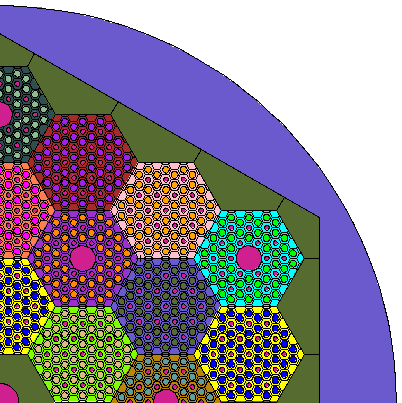
\includegraphics[width=0.60\linewidth]{figures/mcnp-diagram-1}
  \end{center}
  \caption{Quarter section of the $\mu$HTGR core.}
  \label{fig:model-1}
\end{figure}

% The compact
A column of fuel compacts fills out each fuel channel.
The compacts are made of SiC, have a density of 3.2 g/cm$^3$, and hold TRISO particles with a 40\% packing fraction.
The model considers the particles to be uniformly distributed with a particle pitch of 0.1 cm.
Table \ref{table:description} summarizes the characteristics of the TRISO particles.

\begin{table}[!htb]
  \centering
  \caption{TRISO particle definition.}
  \label{table:description} 
  \begin{tabular}{cccc}
  \toprule
   Layer  & Thickness [cm] & Material & Density [g/cm$^3$] \\
  \midrule
   Kernel & 0.0250 & UO2 ($\varepsilon$=19.75\%) & 10.8 \\
   Buffer & 0.0100 & C & 0.98 \\
   IPyC   & 0.0040 & C & 1.85 \\
   SiC    & 0.0035 & SiC & 3.20 \\
   OPyC   & 0.0040 & C & 1.86 \\
  \bottomrule
  \end{tabular}
\end{table}

% SDR calculations
Figure \ref{fig:model-2} displays the side view of the MCNP model.
In the radial direction, the model neglects the presence of the RPV side wall and considers the reactor to be in a cavity of Portland concrete (2.3 g/cm$^3$ density).
The concrete wall is located 191 cm away from the radial reflector and has a 100 cm-thickness.
In the axial direction, the cavity is limited by the citadel floor of Portland concrete with a 70 cm-thickness.
The distance from the top of the reactor to the citadel floor (ground level) is 700 cm.
The remaining volumes are filled with air (80 vol\% nitrogen, 20 vol\% oxygen).

\begin{figure}[htbp!]
  \begin{center}
    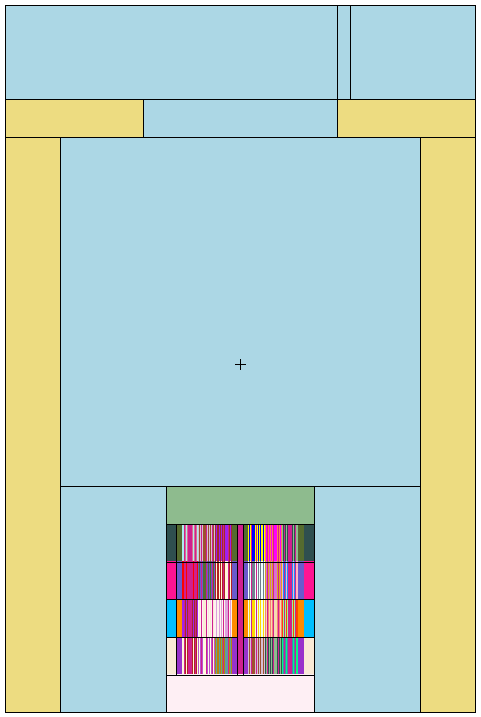
\includegraphics[width=0.40\linewidth]{figures/mcnp-diagram-2}
  \end{center}
  \caption{Side view of the MCNP model including reactor core, reactor cavity, side walls, and citadel.}
  \label{fig:model-2}
\end{figure}

The dose rate is calculated for a worker standing at ground level on the citadel floor.
The calculations use a standard person (often called ``reference man'') of 70 kg weight and 170 cm height, which is represented by an equivalent cylinder.
Considering an average human density of 0.985 g/cm$^3$ yields an equivalent cylinder of 11.53 cm radius.

The calculations consider as radiation sources the fuel in the TRISO particles in all the assemblies and the bottom, top, and radial reflectors.
A sensitivity study determined that the radiation contribution from the fuel particles is approximately 8 orders of magnitude larger than the contribution from the graphite in the assemblies.
The TRISO particle contribution is separated by assembly, for which each assembly has an independent depletion.
% CHANGES IN MCNP INPUT
% To accommodate the MOAA calculations, the MCNP input file took into account the following considerations.
% First, each assembly had an independent material definition in the MCNP input file to allow for their independent depletion.
Finally, the isotope definitions in the MCNP model used the ENDF/B-VIII.0 cross-sections at room temperature.

% Results
% Burnup results
Figure \ref{fig:res-1} displays the $K_{eff}$ time evolution.
The core has an initial $K_{eff}$ of 1.26797 and reaches the end of life at 16.07 years.
Although the original reactor is expected to run for 20 years, the $\mu$HTGR is a simplified version and several of its defining parameters are assumed, as the original parameters are not publicly available.
However, for the purposes of this discussion, the assumptions considered yield an adequate model.

\begin{figure}[htbp!]
  \begin{center}
    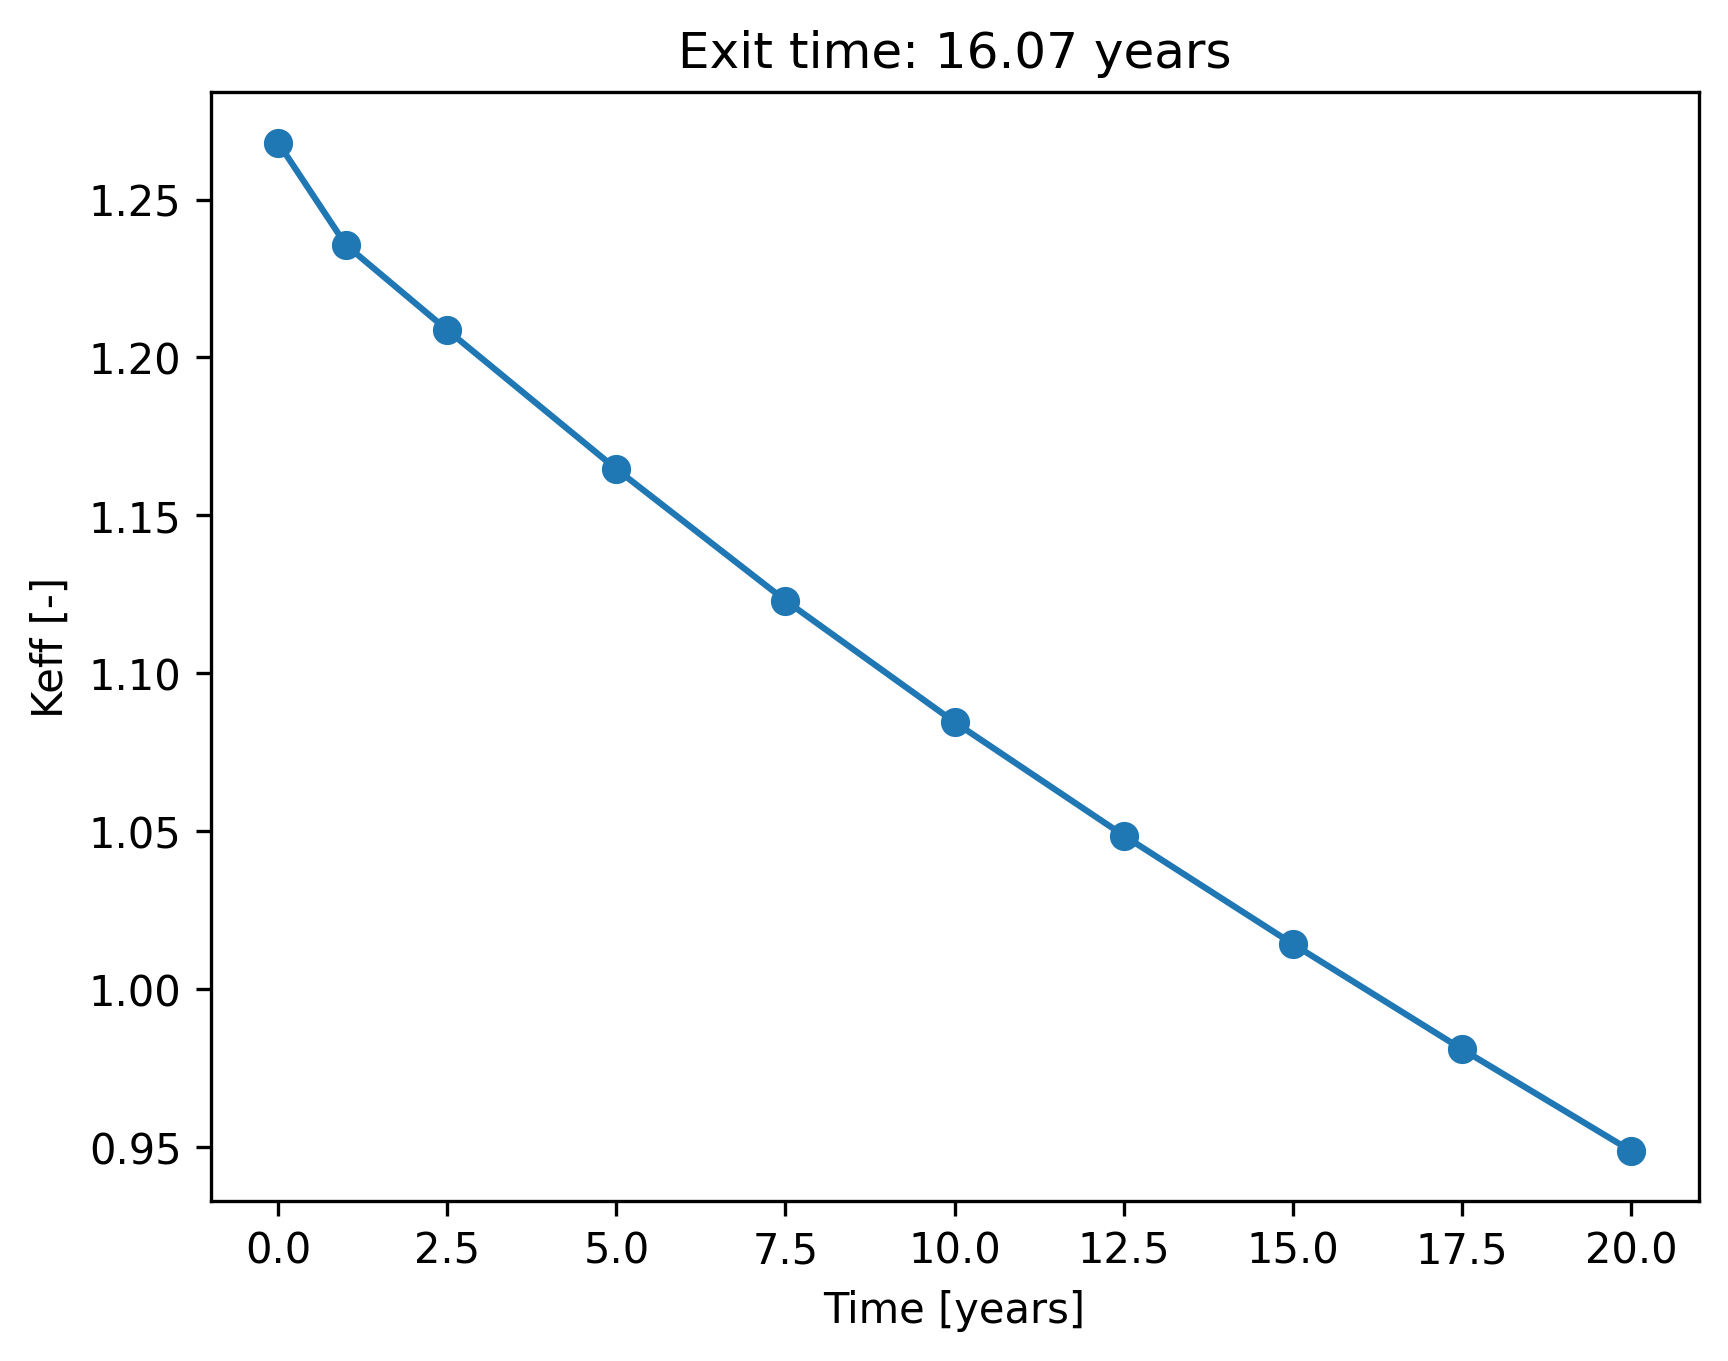
\includegraphics[width=0.55\linewidth]{figures/keff-irrad-time}
  \end{center}
  \caption{$\mu$HTGR $K_{eff}$ time evolution.}
  \label{fig:res-1}
\end{figure}

% heterogenous model results
Figure \ref{fig:res-2} shows the dose rate map at the citadel after a 3-month cool-down.
The region directly above the reactor core shows the largest values, some of them being above 40 mSv/h.
The dose rate in the standard person is 6.48 +/- 1.04 mSv/h.

\begin{figure}[htbp!]
  \begin{center}
    \includegraphics[width=0.60\linewidth]{figures/meshtal4}
  \end{center}
  \caption{Dose rate map at the citadel after 3 month-cool-down.}
  \label{fig:res-2}
\end{figure}

% Discussion
% Title 10, Part 20, of the Code of Federal Regulations (10 CFR Part 20) "Standards for Protection against Radiation".
% https://www.nrc.gov/about-nrc/radiation/health-effects/info.html#dose
The annual total effective dose equivalent for the whole body is 50 mSv for radiation workers.
Although the calculated dose rate is below this limit, other considerations need to be considered, such as exposure time and worker's distance.
These working conditions would allow a radiation worker to perform their tasks for less than 8 hours per year.
Additionally, the calculations consider a vertical distance of 7 m between the top of the core and the worker.
However, while the assemblies are being removed, such a distance will be considerably smaller, and the dose rate will increase accordingly.
For this reason, other decommissioning strategies should be considered to minimize unnecessary exposure.
% Conclusions 10-
Future work should analyze those strategies, adding shielding to the reactor core/assemblies and allowing for a longer cool-down time.


\section{Conclusions}
\label{sec:conclusion}

% Intro
This chapter focuses on the shutdown-dose rate calculations, which are necessary for the determination of suitable \gls*{PIE} strategies for experiment irradiation.
Benefiting from similar workflows, a minimal modification of the workflow allows to obtain both delayed heating and shutdown dose rate.

Motivated by the calculation of shutdown dose rates in experiments, the \gls*{AGR1} experiment sets the path forward for the application of this workflow to \glspl*{HTGR}.
To properly model the AGR-1 experiment, it is insightful to understand the calculation workflow for HTGRs.
% 13- Intro
Additionally, as \gls*{HTGR} technology has distinct features from \glspl*{LWR}, their decommissioning requires new strategies that can be guided by the shutdown dose rate calculations.

% 13- Background
The current available literature on dose rate calculations of HTGRs is scarce, and it focuses on the normal operation regime.
Additionally, previous work on shutdown dose rates of HTGRs lacks the definition of a formal methodology that considers the double heterogeneity of the TRISO fuel.
This thesis introduces a new shutdown dose rate calculation capability for HTGRs that relies on MOAA and the MCNP repeated structures to explicitly model the decay radiation emitted from the TRISO particles.
% 13 - Method
MOAA is responsible for conducting the first two steps of the process, while the third step is conducted by an MCNP photon transport simulation.

% 13- Results
This work introduces a simple exercise to verify the workflow.
For this exercise, one calculation employs the explicit independent definition of each source cell and provides the reference values, while a second calculation utilizes the repeated structures' approach.
% Even though the results for the repeated structures' case show an overestimation of the delayed heating, which is mainly attributed to the problem geometry, the approach seems to yield a reasonable approximation.
The results for the repeated structures' case show that the approach yields a reasonable approximation when the flux spatial variations are considered.

% 13- Results
Finally, this chapter showcases the shutdown dose rate calculation capabilities by presenting two exercises.
These exercises calculate the shutdown dose rate of the AGR-1 TRISO-fueled experiment and a high-temperature gas-cooled microreactor, the $\mu$HTGR.
For the AGR-1 experiment, the results showed that the largest contributor to the dose is the fuel for most decay times.
However, for different decay times, some of the structures produce comparable intensities to the fuel, such as the Hf shroud and the stainless steel structures.
Additionally, the results lead to the recommendation of allowing a decay time of more than one year and the addition of appropriate shielding for conducting the PIE.
For the $\mu$HTGR, the results showed that the proposed decommissioning strategy is feasible but not ideal, as it would lead to very high exposures.
Hence, these results open the door for future studies, which consider the addition of shielding to the reactor core/assemblies and allowing for a longer cool-down time.


\chapter{Generic Irradiation Database}
\label{ch:database}

This chapter investigates different methods to accelerate the delayed heating calculation for experiments of arbitrary material composition.
The most computationally expensive step in the delayed heating calculation is the neutron-transport simulation during experiment irradiation.
This step determines the geometry-dependent parameters, i.e., total neutron flux, neutron spectrum, and reaction rates.
Section \ref{sec:fast} introduces a \textit{fast calculation} method and investigates the possibility of avoiding the repeated run of the neutron-transport simulation to save on computational resources.

Based on the fast calculation results, Section \ref{sec:irradatabase} introduces the \textit{Generic Irradiation Database} method and discusses the results of two applications.
The first application verifies the generic material irradiation database method for the simple demonstration exercise introduced in Section \ref{sec:demo}.
The second application is the verification of the method for an ATR experiment.

\section{Fast Calculation}
\label{sec:fast}

This method solves the neutron-transport problem only once for a specific experiment material to obtain the geometry-dependent parameters.
Then, these parameters are fixed and become the input to the rest of the delayed heating calculation workflow regardless of the experiment composition.
The depletion calculation utilizes these fixed parameters to obtain the charged particle heating and photon source intensity.
The method underlying assumption is that the experiment volume is small enough to perturb the neutron flux in the reactor, and that for all experiment materials the neutron flux is approximately the same.
% As shown in Figure \ref{fig:atr-flux}, the total neutron flux in experiments of different chemical elements is bounded between 3.4 to 6.0 $\times$ 10$^{14} n/cm^2/s$.
As shown in Figure \ref{fig:atr-flux}, the total neutron flux in experiments of different chemical elements is bounded between 3.2 to 5.1 $\times$ 10$^{14} n/cm^2/s$.
These results show that the total neutron flux in the experiment does not vary strongly and always remains in the same order of magnitude.
As the first step of the delayed heating calculation obtains the neutron flux, fixing its value within the range shown in the figure may allow for a sufficiently accurate delayed heating calculation.

\begin{figure}[htbp!]
  \begin{center}
    \includegraphics[width=0.60\linewidth]{figures/demo-materials-flux}
  \end{center}
  \caption{Total neutron flux vs. atomic number of the experiment material.}
  \label{fig:atr-flux}
\end{figure}

As the neutron-transport simulation must be run at least once to fix the geometry-dependent parameters, the question that remains unanswered is what experiment material should be chosen for the simulation.
Two materials are studied: one that considerably perturbs the flux, which is 20\%-enriched uranium, and one that barely perturbs the flux, which is carbon.
Although not shown here, when utilizing the geometry-dependent parameters from the neutron-transport simulation for an experiment of uranium, the delayed heating results are not accurate.
That is because perturbing the reactor flux to obtain the fixed geometry-dependent parameters is not desirable as originally expected.
When perturbing the flux, as the reactor power remains constant, the flux in the experiment increases, while the flux in the fuel assemblies decreases.
Hence, the fuel assemblies are subject to a lower depletion, and consequently they produce a lower delayed gamma emission rate.
As a result, choosing carbon as the experiment material is more favorable because it does not considerably perturb the flux.

To better understand the effects of the geometry-dependent parameters on the delayed heating, this section presents a sensitivity analysis on some key magnitudes in the calculation workflow, i.e., the energy deposited by charged particles ($H_{ch}$) and the photon emission rate ($S_i$).
The calculations use the demonstration exercise from Section \ref{sec:demo}.
The reference calculation is based on the delayed heating calculation workflow for an  experiment of arbitrary material, while the fast calculation uses the values from the neutron-transport simulation for the experiment of carbon.
Figures \ref{fig:sens-al} to \ref{fig:sens-w} show a sensitivity analysis of the $H_{ch}$ and $S_i$ for different total flux levels and selected experiment materials.
These results show that the fast calculation overestimates the results for all cases.
The overestimation for the experiment of aluminum is minimal, while the overestimation for other cases, such as the experiment of enriched uranium, is relatively large.

\begin{figure}[htbp!] % or H
  \centering
  \begin{subfigure}[b]{0.49\textwidth}
    \centering
    \includegraphics[width=0.7\textwidth]{figures/fast-res13_hch}
    \caption{Energy deposited by charged particles.}
  \end{subfigure}
  \hfill
  \begin{subfigure}[b]{0.49\textwidth}
    \centering
    \includegraphics[width=0.7\textwidth]{figures/fast-res13_Si}
    \caption{Photon emission rate.}
  \end{subfigure}
  \hfill
  \caption{Sensitivity analysis for aluminum.}
  \label{fig:sens-al}
\end{figure}

\begin{figure}[htbp!] % or H
  \centering
  \begin{subfigure}[b]{0.49\textwidth}
    \centering
    \includegraphics[width=0.7\textwidth]{figures/fast-res25_hch}
    \caption{Energy deposited by charged particles.}
  \end{subfigure}
  \hfill
  \begin{subfigure}[b]{0.49\textwidth}
    \centering
    \includegraphics[width=0.7\textwidth]{figures/fast-res25_Si}
    \caption{Photon emission rate.}
  \end{subfigure}
  \hfill
  \caption{Sensitivity analysis for manganese.}
  \label{fig:sens-mn}
\end{figure}

\begin{figure}[htbp!] % or H
  \centering
  \begin{subfigure}[b]{0.49\textwidth}
    \centering
    \includegraphics[width=0.7\textwidth]{figures/fast-res40_hch}
    \caption{Energy deposited by charged particles.}
  \end{subfigure}
  \hfill
  \begin{subfigure}[b]{0.49\textwidth}
    \centering
    \includegraphics[width=0.7\textwidth]{figures/fast-res40_Si}
    \caption{Photon emission rate.}
  \end{subfigure}
  \hfill
  \caption{Sensitivity analysis for zirconium.}
  \label{fig:sens-zr}
\end{figure}

\begin{figure}[htbp!] % or H
  \centering
  \begin{subfigure}[b]{0.49\textwidth}
    \centering
    \includegraphics[width=0.7\textwidth]{figures/fast-res74_hch}
    \caption{Energy deposited by charged particles.}
  \end{subfigure}
  \hfill
  \begin{subfigure}[b]{0.49\textwidth}
    \centering
    \includegraphics[width=0.7\textwidth]{figures/fast-res74_Si}
    \caption{Photon emission rate.}
  \end{subfigure}
  \hfill
  \caption{Sensitivity analysis for tungsten.}
  \label{fig:sens-w}
\end{figure}

\begin{figure}[htbp!] % or H
  \centering
  \begin{subfigure}[b]{0.49\textwidth}
    \centering
    \includegraphics[width=0.7\textwidth]{figures/fast-res92_4_4_hch}
    \caption{Energy deposited by charged particles.}
  \end{subfigure}
  \hfill
  \begin{subfigure}[b]{0.49\textwidth}
    \centering
    \includegraphics[width=0.7\textwidth]{figures/fast-res92_4_4_Si}
    \caption{Photon emission rate.}
  \end{subfigure}
  \hfill
  \caption{Sensitivity analysis for 20\%-enriched uranium.}
  \label{fig:sens-u}
\end{figure}

% Results
Table \ref{tab:fast-calc} compares the results using the fast calculation and the reference results obtained using the delayed heating calculation workflow.
The fast calculation method overestimates the delayed heating.
And while for some materials, such as aluminum and zirconium, the overestimation is minimal, for other materials, such as manganese, tungsten, and uranium, the overestimation is considerably larger.
The last step in the comparison is the delayed heating over time, shown in Figures \ref{fig:time-1} to \ref{fig:time-3}.
The delayed heating results confirm the observations in the sensitivity analysis, shown above.
The fast calculation yields accurate results for aluminum and zirconium, while it overestimates the delayed heating in experiments of manganese, tungsten, and uranium.

% Table
\begin{table}[htbp!]
  \centering
  \caption{Comparison of total heat deposited in experiments of selected materials for the fast calculation and the reference results of the delayed heating calculation workflow.}
  \label{tab:fast-calc}
  \begin{tabular}{ccccc}
    \toprule
    Material     & Atomic Number  & Fast [W]   & Reference [W]   & Rel. Diff. [\%] \\
    \midrule
    Aluminum     & 13             & 18.35      & 18.20           & 0.87            \\
    Manganese    & 25             & 375.1      & 169.37          & 121.49          \\
    Zirconium    & 40             & 38.36      & 38.24           & 0.31            \\
    Tungsten     & 74             & 356.19     & 164.46          & 116.58          \\
    Uranium ($\varepsilon$ = 20\%) & 92  & 5880.80  & 994.52     & 491.31          \\
    \bottomrule
  \end{tabular}
\end{table}

\begin{figure}[htbp!] % or H
  \centering
  \begin{subfigure}[b]{0.49\textwidth}
    \centering
    \includegraphics[width=0.7\textwidth]{figures/fast-13_overtime}
    \caption{Aluminum.}
  \end{subfigure}
  \hfill
  \begin{subfigure}[b]{0.49\textwidth}
    \centering
    \includegraphics[width=0.7\textwidth]{figures/fast-25_overtime}
    \caption{Manganese.}
  \end{subfigure}
  \hfill
  \caption{Comparison of the delayed heating over time for the reference workflow and the fast calculation for experiments of selected materials.}
  \label{fig:time-1}
\end{figure}

\begin{figure}[htbp!] % or H
  \centering
  \begin{subfigure}[b]{0.49\textwidth}
    \centering
    \includegraphics[width=0.7\textwidth]{figures/fast-40_overtime}
    \caption{Zirconium.}
  \end{subfigure}
  \hfill
  \begin{subfigure}[b]{0.49\textwidth}
    \centering
    \includegraphics[width=0.7\textwidth]{figures/fast-74_overtime}
    \caption{Tungsten.}
  \end{subfigure}
  \hfill
  \caption{Comparison of the delayed heating over time for the reference workflow and the fast calculation for experiments of selected materials.}
  \label{fig:time-2}
\end{figure}

\begin{figure}[htbp!]
  \begin{center}
    \includegraphics[width=0.42\linewidth]{figures/fast-92_4_4_overtime}
  \end{center}
  \caption{Comparison of the delayed heating over time for the reference workflow and the fast calculation for an experiment of 20\%-enriched uranium.}
  \label{fig:time-3}
\end{figure}

% Conclusion
These results show that the fast calculation is accurate for some cases and excessively conservative for others.
While a conservative approach may be desirable for some cases, this thesis investigates more accurate calculation methods.
Consequently, this section shows that the fast calculation is not suitable for this work's objectives, concluding that the neutron-transport simulations cannot be avoided.
The next section introduces a different approach and investigates its suitability.


\section{Generic Material Irradiation Database}
\label{sec:irradatabase}

% Intro to method
This section proposes the creation of a generic material irradiation database to decrease the burden of the delayed heating calculation in research reactor experiments.
The database is created by utilizing the calculation workflow defined in Chapter \ref{ch:delayedheat} repeatedly to obtain the delayed heating in experiments composed of pure chemical elements.
Nevertheless, an experiment is usually made of a mix of materials.
Hence, this work establishes a method using the database to calculate the delayed heating in experiments of arbitrary material composition.
This method enables the delayed heating calculation based on pre-computed values instead of re-doing the calculations.

% The following formula calculates the delayed heating in an experiment composed of several materials
% \begin{align}
% H_{j,M} &= \mathlarger{\sum}_i H_{j,i}(\rho_i)  \label{eq:data-1} \\
% H_{j,i}(\rho_i) &= \rho_i f(\rho_i)  \label{eq:data-2} \\
% f_{non-fiss}(\rho_i) &= H_{j,i}^o / \rho_i^o  \label{eq:data-3} \\
% f_{fiss}(\rho_i) &= H_{j,i}^k / \rho_i^k  \label{eq:data-4}
% \end{align}
% where $H_{j, M}$ is the heating component $j$ of the mix and $\rho$ is the density.
% The heating component $j$ could be either the charged particles, transported gammas, or total contributions.
% $H_{j,i}$ and $\rho_i$ correspond to the heating values and density of material $i$ in the mix.
% The formula contemplates two cases, fissile and non-fissile materials.
% The calculation of $H_{j,i}(\rho_i)$ requires a functional form for $f(\rho_i)$, being constant for non-fissile (Eq. \ref{eq:data-3}) and density-dependent for fissile materials (Eq. \ref{eq:data-4}).
% $H_{j,i}^o$ corresponds to the heating values for an experiment made of material $i$ only with a density value equal to its theoretical density $\rho_i^o$.
% $H_{j,i}^k$ corresponds to the heating values for an experiment made of material $i$ only with a density value equal to $\rho_i^k$.
% As $f_{fiss}$ is density-dependent, it requires multiple samples of $H_{i,j}^k/\rho_i^k$ for interpolating between adjacent values.

The following formula calculates the delayed heating in an experiment composed of several materials
\begin{align}
H_{j,M} &= \mathlarger{\sum}_i H_{j,i}(m_i)  \label{eq:data-1} \\
H_{j,i}(m_i) &= m_i f(m_i)  \label{eq:data-2} \\
f_{non-fiss}(m_i) &= H_{j,i}^o / m_i^o  \label{eq:data-3} \\
f_{fiss}(m_i) &= H_{j,i}^k / m_i^k  \label{eq:data-4}
\end{align}
where $H_{j, M}$ is the heating component $j$ of the mix, which could be either the charged particles, transported gammas, or total contributions.
$H_{j,i}$ and $m_i$ correspond to the heating values and mass of material $i$ in the mix.
The formula contemplates two cases: fissile and non-fissile materials.
The calculation of $H_{j,i}(m_i)$ requires a functional form for $f(m_i)$, being constant for non-fissile (Equation \ref{eq:data-3}) and mass-dependent for fissile materials (Equation \ref{eq:data-4}).
$H_{j,i}^o$ corresponds to the heating values for an experiment made of material $i$ and mass $m_i^o$, which is the mass of an experiment with density equal to the material's theoretical density $\rho_i^o$.
$H_{j,i}^k$ corresponds to the heating values for an experiment made of material $i$ and mass $m_i^k$, which is an arbitrary value.
As $f_{fiss}$ is mass-dependent, it requires multiple samples of $H_{i,j}^k/m_i^k$ for interpolating between adjacent values.

Because the Equations \ref{eq:data-2} to \ref{eq:data-4} consider a mass ratio, when the volume of the database and the experiment is the same, the mass ratio can be simplified into a density ratio.
The following exercises consider this case, and the calculations are based on the experiment density instead of experiment mass.

% TODO: Need to talk about the combination of fissile material. What results to show ?


\subsection{Demonstration exercise}

The exercise configuration and dimensions can be found in Section \ref{sec:demo}.
The experiment is irradiated for a period of 50 days with the reactor operating at a constant power of 5 MWth.
After that period, the reactor shuts down, and the heat deposited in the experiment is calculated immediately after shutdown.
To avoid the prompt-gamma contributions (emitted within 5 $\times$ 10$^{-8}$ seconds \cite{ilas_impact_2013}), the first step is taken 1 second after shutdown.
The reactor regions considered contributing to the experiment heating are the fuel elements and the experiment itself, while the activation of the moderator is neglected.

% Results from 14-
% Bronze
The following analyses focus on the delayed heating calculation for a mix of materials.
The first analysis considers an experiment of an arbitrary alloy: bronze, which is an alloy of copper and tin.
Bronze has a density of 8.73 g/cm$^3$, and the weight fractions are 88\% and 12\% for copper and tin, respectively.
Table \ref{tab:demo-brz} summarizes the results for the energy deposited by charged particles ($H_{ch}$), energy deposited by photon transport ($H_{\gamma, Tr}$), and total heat deposited ($H_{T}$).
The results from the generic material irradiation database method are based on the delayed heating of samples of pure copper (8.96 g/cm$^3$) and pure tin (5.75 g/cm$^3$).
The calculated values coincide with the reference values.
The relative difference for $H_{ch}$ is the largest, but it is still smaller than 5\%.

\begin{table}[htbp!]
  \centering
  \caption{Comparison of delayed heating for the generic material irradiation database method and reference calculation for an experiment of bronze.}
  \label{tab:demo-brz}
  \begin{tabular}{cccc}
    \toprule
                    & \multicolumn{1}{c}{\begin{tabular}[c]{@{}c@{}}Irradiation  database\\method [W]\end{tabular}} & \multicolumn{1}{c}{\begin{tabular}[c]{@{}c@{}}Reference\\calculation [W]\end{tabular}} & Rel. Diff [\%] \\
    \midrule
    $H_{ch}$            & 15.54   & 16.24   & -4.31  \\
    $H_{\gamma, Tr}$    & 49.75   & 50.17   & -0.84  \\
    $H_{T}$             & 65.30   & 66.41   & -1.67  \\
    \bottomrule
  \end{tabular}
\end{table}

% Bronze, why it works
The following analysis demonstrates why a constant function representing $f_{non-fiss}$ yields a good approximation.
Figure \ref{fig:H_rho1} displays $H_{j,i}/\rho_i$ as a function of $\rho$ for experiments of copper and tin.
The densities considered for copper are 2.25, 4.5, 6.75, and 8.96 g/cm$^3$ and for tin 1.5, 3.0, 4.5, and 5.75 g/cm$^3$.
These values represent approximately 25, 50, 75, and 100\% of the theoretical density for each material.
$H_{ch}$ represents less than 30\% and less than 2\% of $H_T$ for all densities for copper and tin, respectively.
For copper, the slope formed between the first and last values are -24\%, -9\%, and -13\% for $H_{ch}$, $H_{\gamma, Tr}$, and $H_{T}$, respectively.
For tin, the slope formed between the first and last values are -14\%, -16\%, and -16\% for $H_{ch}$, $H_{\gamma, Tr}$, and $H_{T}$, respectively.
The methodology introduced in this paper considers $H_{j,i}/\rho_i$ to be constant for non-fissile materials, as described by Equation \ref{eq:data-3}.
Although these curves have negative slopes, their magnitudes are relatively small, and as shown in Table \ref{tab:demo-brz}, a constant function still yields satisfactory results.

% H/\rho for non-fissile material
\begin{figure}[htbp!] %or H 
    \centering
    \includegraphics[width=0.55\linewidth]{figures/toy-Cu_Sn_rho}
    \hfill
    \caption{$H_{j}/\rho$ vs. $\rho$ for different experiment materials.}
    \label{fig:H_rho1}
\end{figure}

The following exercise considers an experiment including a fissile material, uranium nitride (UN).
This type of fuel has been extensively studied as one candidate accident tolerant fuel, due to its high thermal conductivity and high fissile element density \cite{un}.
Table \ref{tab:demo-un} summarizes the results for an experiment of UN.
The exercise adopts a 4\% enrichment for uranium.
The results from the generic material irradiation database correspond to the calculated value for uranium using a linear interpolation between database entries, while the contribution from nitrogen is considered negligible.
$H_T$ is calculated by adding together $H_{ch}$ and $H_{\gamma,Tr}$.
The relative difference of the results is less than 3\%, which confirms the choice of a linear interpolation to represent $f_{fiss}(\rho_i)$.

\begin{table}[htbp!]
  \centering
  \caption{Comparison of delayed heating for the generic material irradiation database method and reference calculation for an experiment of UN.}
  \label{tab:demo-un}
  \begin{tabular}{cccc}
    \toprule
                    & \multicolumn{1}{c}{\begin{tabular}[c]{@{}c@{}}Irradiation database\\method [W]\end{tabular}} & \multicolumn{1}{c}{\begin{tabular}[c]{@{}c@{}}Reference\\calculation [W]\end{tabular}} & Rel. Diff [\%] \\
    \midrule
    $H_{ch}$            & 273.1   & 267.0   &  2.3  \\
    $H_{\gamma, Tr}$    & 233.7   & 236.0   & -0.9  \\
    $H_{T}$             & 506.8   & 503.0   &  0.8  \\
    \bottomrule
  \end{tabular}
\end{table}

% UN, why it works
The following analysis demonstrates why the inclusion of a fissile material into the mix requires a linear interpolation between database entries to obtain $f_{fiss}$.
The exercise adopts the following uranium densities for the calculations: 1, 7, 13, and 19 g/cm$^3$.
The UN has a density of 13.5 g/cm$^3$, and the atomic fraction is 50\% for both elements.
Figure \ref{fig:H_rho2} displays $H_{j,i}/\rho_i$ as a function of $\rho$ for the experiment of uranium.
Only the values for the uranium are included because the delayed heating in a sample of pure nitrogen is negligible.
$H_{\gamma, Tr}/\rho$ is almost constant, while $H_{ch}/\rho$ decreases as the density increases.
% % Quadratic function R^2: 0.99
% % 0.07013153878082601 x^2 + -2.6293650151097636 x + 42.73063110509705

\begin{figure}[htbp!] %or H 
    \centering
    \includegraphics[width=0.55\linewidth]{figures/toy-U_rho}
    \hfill
    \caption{$H_{j}/\rho$ vs. $\rho$ for an experiment of 4\%-enriched uranium.}
    \label{fig:H_rho2}
\end{figure}

% Zirconium alloys
The following exercise considers three experiments of zirconium alloys: Zircaloy-2, Zircaloy-4, and ZrNb.
% Talk about the importance of these 3 alloys
Zirconium is a metal with excellent corrosion resistance, good mechanical properties, and very low thermal neutron cross-section \cite{zircaloy}.
Zircaloy-2 is composed of Zr-1.5Sn-0.15Fe-0.1Cr-0.05Ni and its primary use is as fuel cladding in \glspl*{BWR} and as calandria tubes in CANDU reactors.
Zircaloy-4 is composed of Zr-1.5Sn-0.2Fe-0.1Cr, which is a similar composition to Zircaloy-2 but removes the nickel and increases the iron weight for less hydrogen uptake, and it is used as fuel cladding in \gls*{PWR} and CANDU reactors.
ZrNb is composed of Zr-2.5Nb, wherein the niobium increases the alloy's strength, and it is used in pressure tubes in CANDU reactors.
%
Table \ref{tab:demo-zircaloy} displays the results for the three zirconium alloys.
The results from the generic material irradiation database method are based on the delayed heating of samples of pure zirconium (7.13 g/cm$^3$), pure tin (5.75 g/cm$^3$), pure iron (7.87 g/cm$^3$), pure chromium (7.18 g/cm$^3$), pure nickel (8.90 g/cm$^3$), and pure niobium (8.57 g/cm$^3$).
The reference calculation considers an experiment density of 6.56 g/cm$^3$, 6.56 g/cm$^3$, and 6.44 g/cm$^3$, for Zircaloy-2, Zircaloy-4, and ZrNb, respectively.
The calculated values show good agreement with respect to the reference values.
The relative difference for $H_{ch}$ is the largest for Zircaloy-2, while all the other relative differences are below 3\%.

\begin{table}[htbp!]
  \centering
  \caption{Comparison of delayed heating for the generic material irradiation database method and reference calculation for multiple experiments.}
  \label{tab:demo-zircaloy}
  \begin{tabular}{cccc}
    \toprule
                    & \multicolumn{1}{c}{\begin{tabular}[c]{@{}c@{}}Irradiation Database\\method [W]\end{tabular}} & \multicolumn{1}{c}{\begin{tabular}[c]{@{}c@{}}Reference\\calculation [W]\end{tabular}} & Rel. Diff [\%] \\
    \midrule
    \multicolumn{4}{c}{Zircaloy-2}                    \\
    \midrule
    $H_{ch}$            &  0.19   &  0.18   &  5.84   \\
    $H_{\gamma, Tr}$    & 38.42   & 38.39   &  0.07   \\
    $H_{T}$             & 38.61   & 38.57   &  0.10   \\
    \midrule
    \multicolumn{4}{c}{Zircaloy-4}                    \\
    \midrule
    $H_{ch}$            &  0.19   &  0.19   &  1.48   \\
    $H_{\gamma, Tr}$    & 38.42   & 38.40   &  0.06   \\
    $H_{T}$             & 38.61   & 38.58   &  0.06   \\
    \midrule
    \multicolumn{4}{c}{ZrNb}                          \\
    \midrule
    $H_{ch}$            &  0.19   &  0.19   &  2.49   \\
    $H_{\gamma, Tr}$    & 37.66   & 37.72   & -0.15   \\
    $H_{T}$             & 37.85   & 37.91   & -0.14   \\
    \midrule
    \multicolumn{4}{c}{U(nat)-Mo}                     \\
    \midrule
    $H_{ch}$            & 135.38   & 132.31  &  2.32  \\
    $H_{\gamma, Tr}$    & 196.06   & 191.66  &  2.30  \\
    $H_{T}$             & 331.44   & 323.97  &  2.31  \\
    \midrule
    \multicolumn{4}{c}{U(nat)-Nb}                     \\
    \midrule
    $H_{ch}$            & 129.13   & 127.35  &  1.39  \\
    $H_{\gamma, Tr}$    & 187.82   & 183.92  &  2.12  \\
    $H_{T}$             & 316.94   & 311.27  &  1.82  \\
    \midrule
    \multicolumn{4}{c}{U(20\%)3Si2Al}                 \\
    \midrule
    $H_{ch}$            & 254.96   & 247.48  &  3.02  \\
    $H_{\gamma, Tr}$    &  95.75   & 108.88  &-12.05  \\
    $H_{T}$             & 350.71   & 356.35  & -1.58  \\
    \midrule
    \multicolumn{4}{c}{Tungsten alloy}    \\
    \midrule
    $H_{ch}$            &  21.35   &  22.52  & -5.22  \\
    $H_{\gamma, Tr}$    & 129.20   & 132.33  & -2.37  \\
    $H_{T}$             & 150.54   & 154.85  & -2.78  \\
    \bottomrule
  \end{tabular}
\end{table}

% Uranium alloys
The following exercise considers three experiments containing uranium.
The first two are uranium-based alloys: U-9Mo and U-10Nb.
It is common for fissionable materials to exhibit anisotropic growth during neutron irradiation.
However, alloying uranium with elements such as molybdenum and niobium, causes the alloy to retain the metastable gamma phase during irradiation, and the anisotropic growth can be eliminated \cite{bleiberg_2004}.
% hutagaol_2022 - U3Si2Al
The third experiment is composed of U$_3$Si$_2$/Al, which is a typical material utilized in \gls*{MTR}-fuel plates.
% 
Table \ref{tab:demo-zircaloy} displays the results for the experiments containing uranium.

The calculations consider a natural uranium composition for the experiments of UMo and UNb and a 20\%-enriched uranium for the experiment of U$_3$Si$_2$/Al.
The results from the generic material irradiation database method are based on the delayed heating of samples of pure uranium, pure molybdenum, pure niobium, pure silicon, and pure aluminum.
The exercise adopts the following uranium densities for the calculations: 1, 7, 13, and 19 g/cm$^3$.
For molybdenum, niobium, silicon, and aluminum, the exercise uses densities of 10.22, 8.57, 2.33, and 2.70 g/cm$^3$, respectively.
The reference calculation considers an experiment density of 17.35, 16.51, and 5.76 g/cm$^3$, for UMo, UNb, and U$_3$Si$_2$/Al, respectively.
Most of the calculated values show good agreement with respect to the reference values, showing relative differences below 3\%, except $H_{ch}$ and $H_{\gamma, Tr}$ for U$_3$Si$_2$/Al.
The latter shows a relative difference of approximately 12\%, but as the charged particles have a larger contribution to the heating, the total heat is within 2\% of the reference value.

% Tungsten alloy
The following exercise considers an experiment of tungsten-nickel-iron alloy.
% 
Tungsten alloys are good candidates for fusion applications, due to tungsten's high melting point.
However, tungsten alone can be very brittle, and including small amounts of other metals, such as nickel and iron, creates a tougher alloy while retaining the high melting temperature \cite{wong_metals_2023}.
The alloy composition considered in this work is W-3.5Ni-1.5Fe.
%
Table \ref{tab:demo-zircaloy} displays the results for this alloy.
The calculated values show good agreement with respect to the reference values.
The largest relative difference is for $H_{ch}$, being around 5\%, while the rest of the relative differences are within 3\%.
% The largest contribution to the delayed heating comes from the gamma particles.

% % FeCrAl
% The following exercise considers two experiments of iron-chromium-aluminum (FeCrAl) alloys.
% % Talk about the importance of this alloy
% This type of alloy exhibits enhanced oxidation resistance in elevated temperature steam environments when compared to Zr-based alloys, making it a good cladding candidate for accident tolerant fuel in \glspl{LWR} \cite{field_accident_2017}.
% Additionally, it is stress corrosion cracking resistant and irradiation induced swelling resistant.
% The typical content ranges from 10 to 22\% for Cr, and from 4 to 8\% for Al.
% This exercise uses the following two compositions: Fe-22\%Cr-8\%Al and Fe-10\%Cr-4\%Al.

% %
% Table \ref{tab:demo-FeCrAl} displays the results for these two alloys.
% The results from the database method are based on the delayed heating of samples of pure Fe ($\rho_{Fe}$ = 7.87 g/cm$^3$), pure Cr ($\rho_{Cr}$ = 7.18 g/cm$^3$), and pure Al ($\rho_{Al}$ = 2.70 g/cm$^3$).
% The reference calculations consider an experiment density of 8 g/cm$^3$ for both alloys.
% The calculated values for $H_{\gamma, Tr}$ and $H_{T}$ show good agreement with respect to the reference values.
% The relative difference for $H_{ch}$ is the largest, being approximately 23\% for the first alloy.
% Because the material is not highly activated, this large relative difference does not affect the total heat deposition, having a relative difference below 1\%.

% \begin{table}[htbp!]
%   \centering
%   \caption{.}
%   \label{tab:demo-FeCrAl}
%   \begin{tabular}{cccc}
%     \toprule
%                     & \multicolumn{1}{c}{\begin{tabular}[c]{@{}c@{}}Database\\method [W]\end{tabular}} & \multicolumn{1}{c}{\begin{tabular}[c]{@{}c@{}}Reference\\calculation [W]\end{tabular}} & Rel. Diff [\%] \\
%     \midrule
%     \multicolumn{4}{c}{70\% Fe, 22\% Cr, 8\% Al}      \\
%     $H_{ch}$            &  0.82   &  0.67   & 22.77   \\
%     $H_{\gamma, Tr}$    & 42.23   & 42.00   &  0.56   \\
%     $H_{T}$             & 43.06   & 42.67   &  0.91   \\
%     \multicolumn{4}{c}{86\% Fe, 10\% Cr, 4\% Al}      \\
%     $H_{ch}$            &  0.43   &  0.35   & 21.24   \\
%     $H_{\gamma, Tr}$    & 42.20   & 42.09   &  0.27   \\
%     $H_{T}$             & 42.63   & 42.45   &  0.44   \\
%     \bottomrule
%   \end{tabular}
% \end{table}

% % RAFM
% The following exercise considers an experiment of reduced activation ferritic-martensitic (RAFM) steel, which is a promising material for fusion reactor structural applications due to its properties such as a reduced activation and elastic and thermal properties that do not differ from Grade91 steel, commonly used in power plants because of its low thermal expansion coefficient and high thermal conductivity \cite{tanigawa_2017}.
% This works considers the following composition Fe-9\%Cr–1\%W–0.2\%V–0.1\%Ta for the steel.

% % results
% Table \ref{tab:demo-RAFM} displays the results for this alloy.
% The results from the database method are based on the delayed heating of samples of pure Fe ($\rho_{Fe}$ = 7.87 g/cm$^3$), pure Cr ($\rho_{Cr}$ = 7.18 g/cm$^3$), pure W ($\rho_{W}$ = 19.3 g/cm$^3$), pure V ($\rho_{V}$ = 6.11 g/cm$^3$), and pure Ta ($\rho_{Ta}$ = 16.654 g/cm$^3$).
% The reference calculations consider an experiment density of 7.80 g/cm$^3$ for the alloy.
% The calculated values for $H_{\gamma, Tr}$ and $H_{T}$ show good agreement with respect to the reference values.
% The relative difference for $H_{ch}$ is the largest, being approximately 53\%.
% Because the material is not highly activated, this large relative difference does not affect the total heat deposition, having a relative difference below 2\%.

% \begin{table}[htbp!]
%   \centering
%   \caption{.}
%   \label{tab:demo-RAFM}
%   \begin{tabular}{cccc}
%     \toprule
%                     & \multicolumn{1}{c}{\begin{tabular}[c]{@{}c@{}}Database\\method [W]\end{tabular}} & \multicolumn{1}{c}{\begin{tabular}[c]{@{}c@{}}Reference\\calculation [W]\end{tabular}} & Rel. Diff [\%] \\
%     \midrule
%     \multicolumn{4}{c}{RAFM}         \\
%     $H_{ch}$            &  0.34   &  0.73   & -53.31  \\
%     $H_{\gamma, Tr}$    & 41.27   & 41.70   &  -1.04  \\
%     $H_{T}$             & 41.61   & 42.43   &  -1.94  \\
%     \bottomrule
%   \end{tabular}
% \end{table}

\subsection{ATR experiment}

% prelim
% \section{ATR Nuclear Heating Database Construction}
% ATR database
% % Maybe plot heating values vs Z/A/rho and see if there are any interesting patterns
% % I think these results will require to separate the fissile materials from the non-fissile materials

This exercise focuses on the delayed heating in the A1 experiment position, which is an inner A-hole that is hosted by the neck shim housing.
This work considers for the calculations a total operating power of 110 MWth that is equally distributed among the 5 lobes.
% Irradiation time
The irradiation time is 30 days, and the decay is recorded in eight non-uniformly distributed steps up to 12 hours after shutdown.
% Contributing cells
As the experiment position is in the core region between the fuel assemblies, the calculations assume that the fission products generate a much higher gamma source intensity than the activation products in the neighboring cells.
Hence, the contribution of the reactor components surrounding the experiment is neglected.
The only considered contributors to the heating are all the fuel plates and the experiment itself.
Section \ref{sec:atrexp} provides more details of the model and modeling assumptions.

% Delayed Heating vs Burnup
% From ilas_impact_2013
% As mentioned in Section 4, the heating calculations for each region have been performed using a
% middle of cycle time (15 days into the operating cycle, MOC_15). Choosing this time in the cycle as a
% representative time for the entire cycle is more conservative, as demonstrated in Fig. 13, than
% previous heating calculations [5] performed with fresh fuel and control elements withdrawn at 22 in.
% The heating rate results at MOC_15 are interpreted to be the average heating rate for the entire cycle.
The generic material irradiation database is based on the delayed heating calculation for the \gls*{MOC} values, which is a conservative approach \cite{ilas_impact_2013}.
Each ATR power cycle typically lasts for 40 to 60 days \cite{sterbentz_agr1_2018}, and this work considers an irradiation time of 30 days.

% % The following will not be shown... I think ...
% The following study investigates the effects of burnup on the delayed heating.
% The delayed heating is calculated in two ATR experiment positions: A2 and I5.
% The A1 and I5 experiment positions host an aluminum and a beryllium filler, respectively.
% Figure \ref{fig:dh-bu} shows the delayed heating vs burnup.
% The delayed heating in I5 is higher than in A2.
% This is most likely due to the filler volumes, and I5's filler is larger in size than A2's.
% Additionally, the highest delayed heat occurs after 10 days of irradiation.
% While the delayed heating remains almost constant in the I5 position, the values decrease as the burnup increases in the A2 position.

% Figure \ref{fig:flux-bu} intends to explain the variation of delayed heat with burnup by showing the average neutron flux and total photon intensity in the fuel assemblies closest to the experiment positions.
% For the A2 position, the fuel assembly closest to the experiment is element 10.
% The total photon intensity decreases with respect to burnup.
% The reason for this is the neutron flux distribution in the core.
% Element 10 has the largest neutron flux as it is closest to the reactor center, and hence it burns faster than other assemblies.
% Contrarily, assemblies in the periphery, such as elements 6 and 15, are subject to a lower flux level, and both the neutron flux and total photon intensity increase with burnup.

% \begin{figure}[htbp!]
%   \begin{center}
%     \includegraphics[width=0.90\linewidth]{figures/dh-bu-res3}
%   \end{center}
%   \caption{Delayed heating vs burnup for A2 (cell 22080) and I5 (cell 65008) experiment position.}
%   \label{fig:dh-bu}
% \end{figure}

% \begin{figure}[htbp!] % or H
%   \centering
%   \begin{subfigure}[b]{0.49\textwidth}
%     \centering
%     \includegraphics[width=0.7\textwidth]{figures/dh-bu-res1}
%     \caption{Average neutron flux.}
%   \end{subfigure}
%   \hfill
%   \begin{subfigure}[b]{0.49\textwidth}
%     \centering
%     \includegraphics[width=0.7\textwidth]{figures/dh-bu-res2}
%     \caption{Total photon intensity.}
%   \end{subfigure}
%   \hfill
%   \caption{Magnitudes in the fuel assemblies closest to the experiment positions.}
%   \label{fig:flux-bu}
% \end{figure}

Figure \ref{fig:atr-data} displays $H_j(Z)$ and $H_j(\rho)$ for all the chemical elements included in the irradiation database.
$H_j(M)$ was plotted as well but the plot is not presented here.
As the relationship between $Z$ and $M$ is linear, the plots are very similar, and $H_j(M)$ does not convey any further information.
$H_{\gamma, Tr}(Z)$ increases with an increasing Z, but not monotonically.
For example, bromine (Z=35), cesium (Z=55), and mercury (Z=80) have lower heating values than the subsequent materials.
$H_{ch}(Z)$ does not present a clear trend with respect to Z.
The general trend for $H_j(\rho)$ is to increase with an increasing $\rho$.
This trend is clearer for the transported photon component than for the charged particle component.
$H_{ch}(\rho)$ is close to zero for densities smaller than 5 g/cm$^3$, has an increasing trend after 15 g/cm$^3$, and oscillates between 0 and 2 kW for the intermediate values.

\begin{figure}[htbp!] % or H
  \centering
  \begin{subfigure}[b]{0.49\textwidth}
    \centering
    \includegraphics[width=0.95\textwidth]{figures/data-H_Z}
    \caption{$H_j(Z)$.}
  \end{subfigure}
  \hfill
  \begin{subfigure}[b]{0.49\textwidth}
    \centering
    \includegraphics[width=0.95\textwidth]{figures/data-H_rho}
    \caption{$H_j(\rho)$.}
  \end{subfigure}
  \hfill
  \caption{Generic material irradiation database values for the ATR A1 experiment position.}
  \label{fig:atr-data}
\end{figure}

% Results from 14-
% Results
% Zircaloy-2
Figure \ref{fig:atr-time-zirc} presents the experiment heat production over time in an experiment of Zircaloy-2.
The reference curve is for an experiment of Zircaloy-2 with a density of 6.56 g/cm$^3$ and the following composition Zr-1.5Sn-0.15Fe-0.1Cr-0.05Ni.
The calculated curve corresponds to the results from the database method and are based on the delayed heating of samples of pure zirconium (7.13 g/cm$^3$), pure tin (5.75 g/cm$^3$), pure iron (7.87 g/cm$^3$), pure chromium (7.18 g/cm$^3$), and pure nickel (8.90 g/cm$^3$).
The delayed heating is 2.36 kW 1 second after shutdown, which is less than 0.01 \% of the total power during operation, and it decays below 500 W within 2 hours.
The calculated curve shows good agreement with the reference curve, having a relative difference smaller than 1\%.

\begin{figure}[htbp!] %or H 
    \centering
    \includegraphics[width=0.60\linewidth]{figures/zircaloy2-tot-vs-t}
    \hfill
    \caption{Heat production over time in an experiment of Zircaloy-2.}
    \label{fig:atr-time-zirc}
\end{figure}

% decay step 0
% \begin{table}[htbp!]
%   \centering
%   \caption{.}
%   \label{tab:atr-zircaloy}
%   \begin{tabular}{cccc}
%     \toprule
%                     & \multicolumn{1}{c}{\begin{tabular}[c]{@{}c@{}}Database\\method [W]\end{tabular}} & \multicolumn{1}{c}{\begin{tabular}[c]{@{}c@{}}Reference\\calculation [W]\end{tabular}} & Rel. Diff [\%] \\
%     \midrule
%     \multicolumn{4}{c}{Zircaloy-2}                        \\
%     $H_{ch}$            &    2.95   &    2.96   & -0.10   \\
%     $H_{\gamma, Tr}$    & 2357.88   & 2345.41   &  0.53   \\
%     $H_{T}$             & 2360.83   & 2348.37   &  0.53   \\
%     \multicolumn{4}{c}{Zircaloy-4}                        \\
%     $H_{ch}$            &    2.95   &    2.96   & -0.29   \\
%     $H_{\gamma, Tr}$    & 2357.86   & 2345.63   &  0.52   \\
%     $H_{T}$             & 2360.82   & 2348.59   &  0.52   \\
%     \multicolumn{4}{c}{ZrNb}                              \\
%     $H_{ch}$            &    2.99   &    3.31   & -9.75   \\
%     $H_{\gamma, Tr}$    & 2307.60   & 2314.60   & -0.30   \\
%     $H_{T}$             & 2310.59   & 2317.92   & -0.32   \\
%     \bottomrule
%   \end{tabular}
% \end{table}

% FeCrAl
The following exercise considers an experiment of iron-chromium-aluminum (FeCrAl) alloy.
This type of alloy exhibits enhanced oxidation resistance in elevated temperature steam environments when compared to Zr-based alloys, making it a good cladding candidate for accident tolerant fuel in \glspl*{LWR} \cite{field_accident_2017}.
Additionally, it is stress corrosion cracking resistant and irradiation induced swelling resistant.
The typical content ranges from 10 to 22\% for chromium, and from 4 to 8\% for aluminum.
Figure \ref{fig:atr-time-fecral} presents the experiment heat production over time in the experiment of FeCrAl.
The reference curve is for an experiment of FeCrAl with a density of 8 g/cm$^3$ and the following composition Fe-22Cr-8Al.
The calculated curve corresponds to the results from the generic material irradiation database method and are based on the delayed heating of samples of pure iron (7.87 g/cm$^3$), pure chromium (7.18 g/cm$^3$), and pure aluminum (2.70 g/cm$^3$).
The delayed heating is 2.38 kW 1 second after shutdown, which is less than 0.01\% of the total power during operation, and it decays below 500 W within 2 hours.
The calculated curve shows good agreement with the reference curve, having a relative difference smaller than 1\%.

\begin{figure}[htbp!] %or H 
    \centering
    \includegraphics[width=0.60\linewidth]{figures/FeCrAl1-tot-vs-t}
    \hfill
    \caption{Heat production over time in an experiment of FeCrAl.}
    \label{fig:atr-time-fecral}
\end{figure}

% decay step 0
% \begin{table}[htbp!]
%   \centering
%   \caption{.}
%   \label{tab:atr-FeCrAl}
%   \begin{tabular}{cccc}
%     \toprule
%                     & \multicolumn{1}{c}{\begin{tabular}[c]{@{}c@{}}Database\\method [W]\end{tabular}} & \multicolumn{1}{c}{\begin{tabular}[c]{@{}c@{}}Reference\\calculation [W]\end{tabular}} & Rel. Diff [\%] \\
%     \midrule
%     \multicolumn{4}{c}{70\% Fe, 22\% Cr, 8\% Al}         \\
%     $H_{ch}$            &   14.87  &   12.21   & 21.80   \\
%     $H_{\gamma, Tr}$    & 2369.97  & 2358.40   &  0.49   \\
%     $H_{T}$             & 2384.84  & 2370.62   &  0.60   \\
%     \multicolumn{4}{c}{86\% Fe, 10\% Cr, 4\% Al}         \\
%     $H_{ch}$            &    7.57  &    6.24   & 21.39   \\
%     $H_{\gamma, Tr}$    & 2374.85  & 2367.56   &  0.31   \\
%     $H_{T}$             & 2382.42  & 2372.80   &  0.36   \\
%     \bottomrule
%   \end{tabular}
% \end{table}

% UMo
The following exercise considers an experiment of UMo with natural uranium.
Figure \ref{fig:atr-time-umo} presents the experiment heat production over time in the experiment of UMo.
The reference curve is for an experiment of UMo with a density of 17.35 g/cm$^3$.
The calculated curve corresponds to the results from the database method and are based on the delayed heating of samples of pure uranium and pure molybdenum.
The exercise adopts the following uranium densities for the calculations: 1, 7, 13, and 19 g/cm$^3$, and a molybdenum density of 10.22 g/cm$^3$.
The delayed heating is 11.29 kW 1 second after shutdown, which is 0.01 \% of the total power during operation, and it decays below 2 kW within 3 hours.
The calculated curve shows good agreement with the reference curve, having a relative difference of approximately 5\%.

\begin{figure}[htbp!] %or H 
    \centering
    \includegraphics[width=0.60\linewidth]{figures/u-mo-tot-vs-t}
    \hfill
    \caption{Heat production over time in an experiment of UMo.}
    \label{fig:atr-time-umo}
\end{figure}

% decay step 0
% \begin{table}[htbp!]
%   \centering
%   \caption{.}
%   \label{tab:atr-Ualloys}
%   \begin{tabular}{cccc}
%     \toprule
%                     & \multicolumn{1}{c}{\begin{tabular}[c]{@{}c@{}}Database\\method [W]\end{tabular}} & \multicolumn{1}{c}{\begin{tabular}[c]{@{}c@{}}Reference\\calculation [W]\end{tabular}} & Rel. Diff [\%] \\
%     \midrule
%     \multicolumn{4}{c}{U(nat)-Mo}         \\
%     $H_{ch}$            &  3507.04   &  3416.95  &  2.64   \\
%     $H_{\gamma, Tr}$    &  7780.91   &  7358.50  &  5.74   \\
%     $H_{T}$             & 11287.95   & 10775.45  &  4.76   \\
%     \multicolumn{4}{c}{U(nat)-Nb}         \\
%     $H_{ch}$            &  3345.27   &  3306.49  &  1.17   \\
%     $H_{\gamma, Tr}$    &  7592.19   &  7156.94  &  6.08   \\
%     $H_{T}$             & 10937.46   & 10463.43  &  4.53   \\
%     \multicolumn{4}{c}{U(20\%)3Si2Al}     \\
%     $H_{ch}$            &  7783.68   &  7527.87  &  3.40   \\
%     $H_{\gamma, Tr}$    &  4690.24   &  4830.27  & -2.90   \\
%     $H_{T}$             & 12473.92   & 12358.14  & -0.94   \\
%     \bottomrule
%   \end{tabular}
% \end{table}


% % Other results
% The following analyses focus on the delayed heating over time for a mix of materials.
% % Bronze
% Figure \ref{fig:atr-time-brz} presents the experiment heat production over time in an experiment of bronze.
% The delayed heating is 2.97 kW 1 second after shutdown, which is less than 0.01 \% of the total power during operation, and it decays to 500 W after approximately 3 hours later.
% The calculated curve shows good agreement with the reference curve, having a relative difference smaller than 2\%.
% The reference curve is for an experiment of bronze with a density of 8.73 g/cm$^3$, and the weight fractions are 88\% and 12\% for copper and tin, respectively.
% The calculated curve corresponds to the results from the database method and are based on the delayed heating of samples of pure copper (8.96 g/cm$^3$) and pure tin (5.75 g/cm$^3$).

% \begin{figure}[htbp!] %or H 
%     \centering
%     \includegraphics[width=0.80\linewidth]{figures/bronze-tot-vs-t}
%     \hfill
%     \caption{Heat production over time in an experiment of bronze.}
%     \label{fig:atr-time-brz}
% \end{figure}

% % decay step 0
% % \begin{table}[htbp!]
% %   \centering
% %   \caption{.}
% %   \label{tab:atr-brz}
% %   \begin{tabular}{cccc}
% %     \toprule
% %                     & \multicolumn{1}{c}{\begin{tabular}[c]{@{}c@{}}Database\\method [W]\end{tabular}} & \multicolumn{1}{c}{\begin{tabular}[c]{@{}c@{}}Reference\\calculation [W]\end{tabular}} & Rel. Diff [\%] \\
% %     \midrule
% %     \multicolumn{4}{c}{Bronze}        \\
% %     $H_{ch}$            &  229.95   &  237.10  & -3.02  \\
% %     $H_{\gamma, Tr}$    & 2743.96   & 2754.34  & -0.38  \\
% %     $H_{T}$             & 2973.91   & 2991.44  & -0.59  \\
% %     \bottomrule
% %   \end{tabular}
% % \end{table}

% \begin{table}[htbp!]
%   \centering
%   \caption{.}
%   \label{tab:atr-sic}
%   \begin{tabular}{cccc}
%     \toprule
%                     & \multicolumn{1}{c}{\begin{tabular}[c]{@{}c@{}}Database\\method [W]\end{tabular}} & \multicolumn{1}{c}{\begin{tabular}[c]{@{}c@{}}Reference\\calculation [W]\end{tabular}} & Rel. Diff [\%] \\
%     \midrule
%     \multicolumn{4}{c}{SiC}        \\
%     $H_{ch}$            &    2.25  &    2.28  & -1.31  \\
%     $H_{\gamma, Tr}$    &  958.36  &  939.10  &  2.05  \\
%     $H_{T}$             &  960.60  &  941.38  &  2.04  \\
%     \bottomrule
%   \end{tabular}
% \end{table}

% \begin{table}[htbp!]
%   \centering
%   \caption{.}
%   \label{tab:atr-ss}
%   \begin{tabular}{cccc}
%     \toprule
%                     & \multicolumn{1}{c}{\begin{tabular}[c]{@{}c@{}}Database\\method [W]\end{tabular}} & \multicolumn{1}{c}{\begin{tabular}[c]{@{}c@{}}Reference\\calculation [W]\end{tabular}} & Rel. Diff [\%] \\
%     \midrule
%     \multicolumn{4}{c}{SS}        \\
%     $H_{ch}$            &   54.70  &   57.28  &  -4.51  \\
%     $H_{\gamma, Tr}$    & 2401.44  & 2402.40  &  -0.04  \\
%     $H_{T}$             & 2456.14  & 2459.68  &  -0.14  \\
%     \bottomrule
%   \end{tabular}
% \end{table}

% \begin{table}[htbp!]
%   \centering
%   \caption{.}
%   \label{tab:atr-w}
%   \begin{tabular}{cccc}
%     \toprule
%                     & \multicolumn{1}{c}{\begin{tabular}[c]{@{}c@{}}Database\\method [W]\end{tabular}} & \multicolumn{1}{c}{\begin{tabular}[c]{@{}c@{}}Reference\\calculation [W]\end{tabular}} & Rel. Diff [\%] \\
%     \midrule
%     \multicolumn{4}{c}{95\%-W, 3.5\%-Ni, 1.5\%-Fe}      \\ % Double check the composition
%     $H_{ch}$            &  310.55  &  329.49  & -5.75   \\
%     $H_{\gamma, Tr}$    & 5463.04  & 5671.29  & -3.67   \\
%     $H_{T}$             & 5773.59  & 6000.78  & -3.79   \\
%     \bottomrule
%   \end{tabular}
% \end{table}

% \begin{table}[htbp!]
%   \centering
%   \caption{.}
%   \label{tab:atr-RAFM}
%   \begin{tabular}{cccc}
%     \toprule
%                     & \multicolumn{1}{c}{\begin{tabular}[c]{@{}c@{}}Database\\method [W]\end{tabular}} & \multicolumn{1}{c}{\begin{tabular}[c]{@{}c@{}}Reference\\calculation [W]\end{tabular}} & Rel. Diff [\%] \\
%     \midrule
%     \multicolumn{4}{c}{RAFM}         \\
%     $H_{ch}$            &    9.01  &   12.66  & -28.83   \\
%     $H_{\gamma, Tr}$    & 2381.76  & 2369.79  &   0.51   \\
%     $H_{T}$             & 2390.77  & 2382.45  &   0.35   \\
%     \bottomrule
%   \end{tabular}
% \end{table}

\section{Conclusions}

% From 14-
% Intro
Safety analyses in research reactors require the estimation of heat deposited in experiments and reactor structures after shutdown.
Research reactors enable the irradiation of a wide variety of unique experiments, requiring the development of safety analyses on a case-by-case basis, which often proves to be effort- and time-consuming.
This chapter studies two methods using previous knowledge to expedite the process.

First, the chapter investigates the feasibility of reducing the calculation burden by solving the neutron-transport problem only once.
This fast method utilizes the geometry-dependent parameters from the neutron-transport problem for an experiment of carbon, which is a material that does not considerably perturb the neutron flux.
Then, the depletion calculation utilizes these parameters to obtain the charged particle heating and photon source intensity.
Some cases are studied for selected materials and the results compared to the results obtained with the delayed heating calculation workflow.
The results show that the fast calculation is accurate for some cases while excessively conservative for others.
Additionally, the study concludes that this approach is not suitable to this thesis' objectives and that neutron-transport simulations cannot be avoided.

Second, this chapter also describes the generic material irradiation database method, which relies on the delayed heating calculation to obtain the heat produced in experiments of individual chemical elements and through their combination calculate the heat produced in experiments of arbitrary material composition.
% Results
Finally, this chapter demonstrates the generic material irradiation database method by presenting two exercises.
These exercises include the delayed heating calculation of experiments for a demonstration exercise and ATR.
The results verify the method by showing a wide variety of combinations of materials that could integrate a research reactor experiment.
Additionally, for the case of the ATR exercise, the heat production over time is shown for several experiments.
Overall, the results exhibit good agreement between the calculated and reference values.

% Future work
% Further investigation is needed to understant the perfomance of this method on experiments comprising a mix of heavy/fissile elements. 

\chapter{Thermal-Fluids and Machine Learning}
\label{ch:tf}

% Describe how this Ch is organized
This chapter examines the applicability of machine learning to capture the behavior of an experiment during the transient provided its thermal properties are known.
Data-based modeling, which relies on machine learning, extracts features from data generated with the physics-based model and predicts the behavior of new data.
Hence, a thermal-fluids solver is necessary to determine the thermal behavior of the experiment and generate the required data to train and test the data-based model.
Section \ref{sec:tf} describes the thermal-fluids solvers utilized in this work.
Additionally, this work compares the performance of different data-based strategies.
Section \ref{sec:ML} introduces briefly the machine learning algorithms utilized in this work, Section \ref{sec:simpl-model} introduces a simplified thermal-fluids model, its verification, and it investigates the performance of the different data-based approaches and machine learning algorithms.
Section \ref{sec:datapros} discusses some necessary changes in the data processing to implement the data-based modeling for an experiment subject to delayed heating.
Finally, Section \ref{sec:atr} demonstrates the data-based modeling of an ATR experiment undergoing the accident.


\section{Thermal-Fluids Solvers}
\label{sec:tf}

\subsection{MOOSE}

% fairhurst-agosta_machine_2_2022
The \gls*{MOOSE} \cite{gaston_moose_2009}, originally released in 2008, is an open-source \gls*{FEM} framework that supports engineering analysis applications, targeting systems of non-linear partial differential equations.
The MOOSE applications define weak forms of the governing equations and modularize the physics expressions into \textit{kernels}.
The kernels are C++ classes containing methods for computing the residual and Jacobian contributions of individual pieces of the governing equations.
All the software built on the MOOSE framework shares the same \gls*{API}.
This feature facilitates a relatively easy coupling between different phenomena.
Additionally, the framework and its applications use \gls*{MPI} for parallel communication and can be deployed on massively parallel cluster-computing platforms.

% MOOSE role in the calculations
In this work, MOOSE solves a simplified thermal-fluids model (Section \ref{sec:simpl-model}) to examine the applicability of machine learning to capture the experiment thermal behavior.
Three reasons motivated the choice of MOOSE for such a study.
First, the author's familiarity with the software made it the natural choice.
% Second, the MOOSE input sequence consists of only one script, while OpenFOAM’s comprises several scripts.
Second, the MOOSE input sequence consists of only one script, which reduces the burden of handling a large number of files.
Third, the MOOSE model uses the Boussinesq approximation to reduce the computational expense of the simulation.
The approximation considers that the density-variation effects are only present in the body force term of the conservation of momentum equations.
% MOOSE / Equations
% fairhurst-agosta_machine_2_2022
This approximation reduces the system of equations in the fluid region to three equations for solving the motion and temperature
% Equations
\begin{align}
& \nabla \cdot \vec{u} = 0 \\
& \rho \left( \frac{\partial \vec{u}}{\partial t} + (\vec{u} \cdot \nabla)\vec{u} \right) + \nabla p - \rho \vec{g} + \rho \vec{g} \beta (T - T_{ref}) - \mu \Delta \vec{u}= 0 \\
& \rho c_p \left( \frac{\partial T}{\partial t} + (\vec{u} \cdot \nabla) T \right) - k \Delta T - q''' = 0  
\end{align}
where $\vec{u}$ is the velocity, $\rho$ is the density, $p$ is the pressure, $\vec{g}$ is the gravity, $\beta$ is the thermal expansion coefficient, $T$ is the temperature, $T_{ref}$ is the reference temperature, $\mu$ is the dynamic viscosity, $c_p$ is the specific heat capacity, and $k$ is the thermal conductivity.
MOOSE solves the heat conduction equation to obtain the temperature in the solid regions
\begin{align}
& \rho c_p \frac{\partial T}{\partial t} - k \Delta T - q''' = 0 \\
& q'''(t)[W/m^3] = q_0 e^{-t/\tau}
\end{align}
where $q'''$ is the heat source which is uniformly distributed across the experiment volume and is defined by a decaying exponential representing the delayed heating.


\subsection{OpenFOAM}

% Equations: solve the air density
% https://caefn.com/openfoam/solvers-buoyantpimplefoam
% More equations:
% https://cfd.direct/openfoam/energy-equation/
% https://doc.cfd.direct/openfoam/user-guide-v6/thermophysical
% https://www.openfoam.com/documentation/guides/latest/api/hConstThermoI_8H_source.html
% https://github.com/OpenFOAM/OpenFOAM-dev/blob/master/src/thermophysicalModels/basic/rhoThermo/heRhoThermo.C
% https://www.cfd-online.com/Forums/openfoam-programming-development/222965-temperature-calculation-enthalpy.html

% fairhurst-agosta_machine_2_2022
OpenFOAM \cite{weller_tensorial_1998} is a \gls*{FVM} C++ class library originally released as the Field Operation And Manipulation (FOAM) library in 1989, becoming open source in 2004.
It comprises an extensible range of libraries, solvers, and pre- and post-processing tools, for which the developers intended to make the top-level syntax of the code as close as possible to conventional mathematical notation.
The result is a C++ class library capable of modeling continuum-mechanics phenomena, such as compressible and incompressible flow, multiphase flow, including various turbulence modeling techniques.
Although it primarily targets \gls*{CFD} problems, it solves other continuum-mechanics problems as well, such as structural mechanics \cite{weller_tensorial_1998} or molecular dynamics \cite{longshaw_mdfoam_2018}.
Moreover, it supports parallelization via domain decomposition, in which each available processor runs the code in each mesh subdomain.

Further inspection of the thermal-fluids model revealed that even when MOOSE uses the Boussinesq approximation and OpenFOAM does not, OpenFOAM simulations are considerably faster.
This reason motivated the choice of OpenFOAM as the main solver for more detailed models.
Furthermore, OpenFOAM has several turbulence models readily available and is capable of solving the density, motion, and temperature of the fluid.

% OpenFOAM calculates the capsule temperature during the channel draining event by solving the mass, momentum, and energy conservation equations (Equation \ref{eq:consv-mass}-\ref{eq:consv-ene-f}) along with the equation of state (Equation \ref{eq:state}) in the air regions, and the heat conduction equation (Equation \ref{eq:consv-ene-s}) to solve the temperature in the solid regions \cite{weller_tensorial_1998}
OpenFOAM calculates the capsule temperature during the channel draining event by solving the mass, momentum, and energy conservation equations along with the equation of state in the air regions, and the heat conduction equation to solve the temperature in the solid regions \cite{weller_tensorial_1998}
\begin{align}
& \frac{\partial}{\partial t} \rho + \nabla \cdot (\rho \bar{u}) = 0  \label{eq:consv-mass} \\
& \left( \frac{\partial}{\partial t} (\rho \bar{u}) + \nabla \cdot \left( \rho \bar{u u} \right) \right) + \nabla p - \rho \bar{g} - \mu \Delta \bar{u} = 0 \label{eq:consv-mom} \\
& \left( \frac{\partial}{\partial t} (\rho h) + \nabla \cdot \left( \rho \bar{u} h \right) \right) + \frac{\partial}{\partial t} \left( \rho \frac{|\bar{u}|^2}{2} \right) + \nabla \cdot \left( \rho \bar{u} \frac{|\bar{u}|^2}{2} \right) - \frac{\partial}{\partial t}p - \alpha \Delta h - \rho \bar{g} \cdot \bar{u} = 0 \label{eq:consv-ene-f} \\
& p = \rho R T \label{eq:state} \\
& h = c_p T \\
& \rho c_p \frac{\partial}{\partial t} T - k \Delta T - q''' = 0 \label{eq:consv-ene-s}
\end{align}
where $\rho$ is the density, $\bar{u}$ is the velocity, $p$ is the pressure, $\bar{g}$ is the gravity, $\mu$ is the dynamic viscosity, $h$ is the enthalpy, $\alpha$ is the thermal diffusivity, $R$ is the ideal gas constant, $c_p$ is the specific heat capacity, $T$ is the temperature, $k$ is the thermal conductivity, and $q'''$ is the volumetric heat source.
While the air and capsule thermal properties are fixed, the experiment thermal properties are defined by the user and are specific to each experiment.
The function for the volumetric heat source is provided by the delayed heating calculation workflow.

% https://openfoamwiki.net/index.php/ChtMultiRegionFoam
% https://www.tfd.chalmers.se/~hani/kurser/OS_CFD_2016/TuroValikangas/Report_Turo.pdf
The calculations use OpenFOAM v2012 (December 2020 release) and the application \textit{chtMultiRegionFoam}.
This application solves transient fluid flow and solid heat conduction with conjugate heat transfer between regions.
The solver follows a segregated solution strategy, wherein the equations for each characteristic variable are solved sequentially and their solution inserted in the subsequent equations.
The coupling between fluid and solid follows a similar approach, wherein the fluid equations are solved using the solid temperatures from the previous iteration as the boundary condition.
Then, the equation for the solid is solved using the temperature of the fluid of the previous iteration as the boundary condition.
And this process is repeated until convergence.

% Turbulence ?
% Radiation Heat Transfer ?

% Fluid regions
% rho
% Ux
% Uy
% Uz
% h
% G
% p_rgh
% rho

% Solid regions
% h

% p_rgh = p - rho g h

% TO DO, need to work a bit more on this explanation

\section{Machine Learning}
\label{sec:ML}

% Classification
This work uses several classification algorithms to determine if the capsule encasing the experiment melts in case of a channel draining event.
Classification is the process of recognizing certain patterns in a dataset and grouping the samples into categories based on those patterns.
Machine learning classification algorithms use training data to determine such categories and then predict the likelihood that subsequent data points will fall into them.
This work utilizes the following classification techniques: \Gls*{SVM}, \Gls*{DT}, \Gls*{RF}, \Gls*{KNN}, \Gls*{LogR}, and \Glspl*{FNN}.

% Regression
Additionally, this work utilizes several methods to predict the time evolution of the capsule temperature.
These methods rely on the following algorithms: \Gls*{DTR}, \Gls*{RFR}, \Glspl*{FNN}, and \Glspl*{LSTM}.
% Packages
The implementation of the FNNs and LSTMs utilizes \textit{Keras} \cite{chollet_keras_2015} and the rest of the models
utilize \textit{scikit-learn} \cite{pedregosa_scikit-learn_2011}.
This section presents a brief introduction to the different machine learning algorithms.


\subsection{Support Vector Machine}

% https://scikit-learn.org/stable/modules/svm.html#mathematical-formulation
% see http://web.mit.edu/6.034/wwwbob/svm-notes-long-08.pdf
% bae_calculation_2008
% fletcher_support_2008

This algorithm searches for a hyperplane that separates the dataset, as shown in Figure \ref{fig:svm}.
The support vectors are a small subset of the training samples that are closest to this hyperplane.
The method determines the hyperplane that maximizes the distance or margin to the support vectors \cite{pedregosa_scikit-learn_2011}.

\begin{figure}[htbp!] %htbp! or H
  \centering
  \includegraphics[width=0.5\linewidth]{figures/svr}
  \caption{Visualization of SVM classification.}
  \label{fig:svm}
\end{figure}

Equation \ref{eq-svm-1} defines the hyperplane, and Equation \ref{eq-svm-2} defines the hyperplanes of the support vectors, where $\phi(x)$ is the transformation from feature to kernel space that allows for non-linear solutions.
The margin between hyperplanes is equal to $1/||w||$, and then maximizing the margin is equivalent to minimizing $||w||$.
The optimization problem is solved by minimizing $J(w)$ in Equation \ref{eq-svm-3}:
\begin{align}
&w \cdot \phi(x_i) + b = 0    \label{eq-svm-1} \\
&w \cdot \phi(x_i) + b = \pm1 \label{eq-svm-2} \\
J(w) &= \frac{1}{2} ||w||^2 + C \sum_i \xi_i \label{eq-svm-3} \\
\intertext{such that}
y_i(&w \cdot \phi(x_i) + b) \geq 1-\xi_i \\
& \xi_i \geq 0
\end{align}
where $C$ is the regularization factor, which gives more weight to minimizing the flatness or the error, $\xi_i$ is the slack variable, which guards against outliers.
Some problems are not perfectly separable with a hyperplane.
The optimization of Equation \ref{eq-svm-3} allows some samples to be at a $\xi_i$ distance from their correct boundary.
A larger regularization parameter penalizes the approximation error, leading to its decrease during the optimization.
% An increase in the regularization parameter leads to a decrease of the approximation error.
% A larger $\epsilon$ decreases the number of support vectors, reducing the accuracy of the approximation.


\subsection{Decision Tree}

% steorts_tree_2017-1
% https://scikit-learn.org/stable/modules/tree.html#mathematical-formulation

The algorithm divides the predictor space into simple regions.
The set of splitting rules segmenting the predictor space can be visualized as an inverted tree, as shown in Figure \ref{fig:dt}.
Its branches connect internal nodes where a test determines in which sub-branch to continue.
The end of the tree contains the leaf nodes which make the final predictions.
The leaf nodes assign the most commonly occurring class of the training observations to new observations falling into those regions.

\begin{figure}[htbp!] %htbp! or H
  \centering
  \includegraphics[width=0.5\linewidth]{figures/dt}
  \caption{Visualization of a decision tree.}
  \label{fig:dt}
\end{figure}

\Gls*{DT} uses a recursive binary split to grow the tree by minimizing an impurity function, which in this case is the Gini index \cite{pedregosa_scikit-learn_2011}, defined as
\begin{align}
& G = \sum_k p_{mk}(1-p_{mk}) \label{eq-dt}
\end{align}
where $p_{mk}$ is the proportion of class $k$ observations in the region node $m$.
A low Gini index indicates that a node contains predominantly observations from a single class.
Other measures of impurity include entropy and misclassification.
The package \textit{scikit-learn} uses the Gini index by default.

%The advantages of \glspl{DT} are that they are easy to interpret and that require little data preparation.
%Their main disadvantage is that complex trees are prone to overfitting.
%Predictions of decision trees are not continuous, but piecewise constant approximations.
%Therefore, they are not good at extrapolation.

% DTR
The algorithm for \gls*{DTR} is slightly different.
The tree can be visualized as a piecewise constant approximation.
For every new observation falling into the same space subregion, the leaf nodes assign the same prediction value, which is the average value of the training observations.
The training algorithm minimizes the \gls*{MSE} \cite{pedregosa_scikit-learn_2011}
\begin{align}
& MSE = \frac{1}{n_m} \sum_{y \in Q_m} \left( y - \bar{y}_m \right)^2 \label{eq-dtr} \\
& \bar{y}_m = \frac{1}{n_m} \sum_{y \in Q_m} y
\end{align}
where $\bar{y}_m$ is the learned mean value of the node.
$Q_m$ represents the data at node $m$ with $n_m$ samples.


\subsection{Random Forest}

% pedregosa_scikit-learn_2011

This method improves the performance of a single tree, as individual DTs may exhibit high variance.
This method reduces the overfitting and increases its precision.
The algorithm consists of a collection of decision trees.
It is based on the bootstrap aggregating method or \textit{bagging} \cite{breiman_bagging_1996}, which chooses the training data for each decision tree at random with replacement, fits the \glspl*{DT}, and then combines their results by voting.
The purpose of the randomness is to decrease the variance of the forest and decouple the prediction error \cite{pedregosa_scikit-learn_2011}.
% RFR
The algorithm for \gls*{RFR} is very similar, but instead of combining the different DT results by voting, the result is an average of the predictions of the different trees.


\subsection{K-Nearest Neighbors}

% https://scikit-learn.org/stable/modules/neighbors.html#classification

Neighbors-based classification does not create a model, but instead it stores instances of the training data \cite{pedregosa_scikit-learn_2011}.
Then, the algorithm classifies new samples based on the stored instances.
The KNNs are the $K$ training observations closest in distance to a new observation.
The Euclidean distance is the most common choice for measuring the distance between observations.
When classifying a new observation, the method assigns the data class which has the most representatives within the nearest neighbors of the point.
\gls*{KNN} is often successful in classification situations where the decision boundary is very irregular.

Figure \ref{fig:knn} displays an example of KNN classification, where the green dot is the sample to classify.
For a K value equal to three, the method uses the three closest samples to the green dot.
Two values are blue, and one is orange.
As the majority of the samples is blue, the method assigns the blue category to the new sample.

\begin{figure}[htbp!] %htbp! or H
  \centering
  \includegraphics[width=0.5\linewidth]{figures/knns}
  \caption{Visualization of KNN classification.}
  \label{fig:knn}
\end{figure}

\subsection{Logistic Regression}

% https://scikit-learn.org/stable/modules/linear_model.html#logistic-regression

This type of regression determines the relationship between a binary dependent variable and a set of independent variables.
The method utilizes the sigmoid function, shown in Equation \ref{eq:logR-1}, to determine the likelihood of an observation to fall within each category.
The method determines the coefficients of the sigmoid function by minimizing a certain cost function.
This work uses the default setting of \textit{scikit-learn} which is to minimize the $L_2$-penalized cost function $J(w)$
% What loss? also, L2 regularization
\begin{align}
& \sigma(x_i) = \frac{1}{1+e^{-(w \cdot x_i + b)}} \label{eq:logR-1} \\
& J(w) = \frac{1}{2} ||w||^2 + C \sum_i log(exp(-y_i(w \cdot x_i + b))+1) \label{eq:logR-2}
\end{align}
where $C$ is the regularization factor.
% Like in support vector machines, smaller values specify stronger regularization.
Like in SVM, a larger regularization factor decreases the approximation error during the optimization.

Figure \ref{fig:logR} displays an example of logistic regression.
Most of the orange samples are located in the lower range of the independent variable $X$ while the blue samples are located in the upper range.
Then, training the model will assign values to the sigmoid function coefficients such that for new samples in the lower range of $X$, it will predict the $0$ category, while for new samples in the upper range of $X$, it will predict the $1$ category.

\begin{figure}[htbp!] %htbp! or H
  \centering
  \includegraphics[width=0.5\linewidth]{figures/LogR}
  \caption{Visualization of logistic regression classification.}
  \label{fig:logR}
\end{figure}


\subsection{Feed-forward Neural Networks}

\Glspl*{FNN} are deep-learning architectures that learn complex relationships between inputs and outputs by mimicking biological networks of neurons.
A network consists of an input and output layer, and $M$ hidden layers of neurons, as shown in Figure \ref{fig:3-fnn}.

\begin{figure}[htbp!] % or H
  \centering
  \begin{subfigure}[b]{0.51\textwidth}
    \centering
    \includegraphics[width=1.0\textwidth]{figures/fnn-1}
    \caption{}
  \end{subfigure}
  \hfill
  \begin{subfigure}[b]{0.47\textwidth}
    \centering
    \includegraphics[width=0.65\textwidth]{figures/fnn-2}
    \caption{}
  \end{subfigure}
  \hfill
  \caption{Example of an FNN.}
  \label{fig:3-fnn}
\end{figure}

A neuron is connected to the neurons of the previous layer by weights.
Each neuron adds together the product of the neuron values in the previous layer and the weights connecting them plus a bias.
This summation serves as input to the next layer after applying an activation function, as stated in the following equation
\begin{align}
& y_{l, i} = f(w_{l, i}^T y_{l-1} + b_{l, i}) \label{eq-fnn-1} \\
& H = -\frac{1}{N} \sum_i y_i log(p(y_i)) + (1 - y_i) log(1 - p(y_i)) \label{eq-fnn-2}
\end{align}
where $y_{l, i}$ is the output of the node $i$ in layer $l$, $y_{l-1}$ output values of layer $l$-$1$, $f$ the activation function, and $w_{l, i}$ and $b_{l, i}$ the weights and biases connecting layer $l$-$1$ to the node $i$ of layer $l$.

Training the network sets the values of the connecting weights and biases by minimizing an error metric.
For the classification problem, the error metric is the binary cross-entropy, shown in Equation \ref{eq-fnn-2}, where $y_i$ is the label, $p(y_i)$ is the predicted probability of the point to be \textit{true}, and $N$ is the number of samples.

% FNNs for regression
When using the FNN for regression, the algorithm trains the network by minimizing the MSE
\begin{align}
MSE = \frac{1}{N} \sum_i (Y_i - \hat{Y_i})^2 \label{eq-MSE}
\end{align}
where $\hat{Y_i}$ is the predicted output of the node $i$ of the output layer of the network, $Y_i$ is the target value, and $N$ is the number of nodes in the output layer times the number of samples.


\subsection{Long-Short Term Memory Networks}
\label{sec:lstm}

% LSTMs
% https://colah.github.io/posts/2015-08-Understanding-LSTMs/
% https://www.analyticsvidhya.com/blog/2021/03/introduction-to-long-short-term-memory-lstm/
Although RNNs are neural networks that handle inputs and outputs correlated as part of a sequence, they cannot learn long-term dependencies.
When training the network, the back-propagated gradients may grow or shrink significantly at each time step.
Therefore, the gradients may vanish or explode for time series with long duration.
LSTMs are a special kind of RNN that were explicitly designed to avoid the vanishing gradient problem and are able to learn long-term dependencies.

% LSTM - Structure
The LSTM cell consists of three parts, better known as gates: the forget gate, the input gate, and the output gate, shown in Figure \ref{fig:lstm}.
The forget gate determines if the information from the previous timestamp is forgotten, the input gate controls the flow of new information, and the output gate updates the information into the next timestamp.
The gates allow the LSTM to add or remove information to the cell state $C_t$ and hidden state $h_t$.
The cell and hidden states are also known as long-term and short-term memory, respectively.

\begin{figure}[htbp!] %htbp! or H
  \centering
  \includegraphics[width=0.5\linewidth]{figures/lstm}
  \caption{LSTM structure.}
  \label{fig:lstm}
\end{figure}

% Equations
The following sets of equations are the mathematical definition of the LSTM cell
\begin{align}
f_t &= \sigma \left( W_f h_{t-1} + U_f x_t + b_f \right)  \label{eq:lstm1} \\
i_t &= \sigma \left( W_i h_{t-1} + U_i x_t + b_i \right)  \label{eq:lstm2} \\
\tilde{C}_t &= tanh \left( W_C h_{t-1} + U_C x_t + b_C \right)  \label{eq:lstm3} \\
C_t &= f_t \cdot C_{t-1} + i_t \cdot \tilde{C}_t          \label{eq:lstm3} \\
o_t &= \sigma \left( W_o h_{t-1} + U_o x_t + b_o \right)  \label{eq:lstm4} \\
h_t &= o_t \cdot tanh \left( C_t \right)                  \label{eq:lstm5}
\end{align}
where $W$ and $b$ are the weights and biases for the different layers as in any other type of network.
The forget gate output $f_t$ is a number between 0 and 1, wherein a value of 0 means forget everything, and a value of 1, forget nothing.
In the input gate, $i_t$ defines which values to update, and $\tilde{C}_t$ comprises the candidate values that can be added into the cell state.
The cell state $C_t$ is calculated as the addition of the values not forgotten from the previous cell state $C_{t-1}$ and the new updated values $\tilde{C}_t$.
Finally, the hidden state $h_t$ is a filtered version of the cell state $C_t$, and $o_t$ decides what information is included.
% This technique is able to consider additional explanatory variables while learning across time-series \cite{calkoen_traditional_2021}.

Overall, the network can be visualized as a mathematical function whose inputs are the time-dependent features $x_t$ which produce the time-dependent outputs $h_t$.
The training of the network is a bit more cumbersome than for other neural networks.
As both the features and outputs are time-dependent, the common training strategy converts the time-dependent problem into a static supervised problem, wherein the output of previous time steps act as input to the next time step.
The supervised problem separates the data into \textit{look-back} and \textit{look-forward} steps.
The look-back steps are the number of steps that the network uses to predict a certain number of look-forward steps at a time.
Figure \ref{fig:lstm-convert} displays an example of the conversion process.
For the output time-series $h$, with $N_t$ time steps, the input and output of the supervised problem take the shape $(N_t-N_{lb}-N_{lf}) \times N_{lb}$ and $(N_t-N_{lb}-N_{lf}) \times N_{lf}$, respectively, where $N_{lb}$ and $N_{lf}$ are the number of look-back and look-forward steps.
Additionally, the network is able to learn a dependency on the features $x_t$ by adding this information to the inputs of the supervised problem.
Assuming static features $x_t = x$, the input of the supervised problem takes the shape $(N_t-N_{lb}-N_{lf}) \times (N_x + N_{lb})$, where $N_x$ is the number of features.

% Conversion from unsupervised to supervised problem
% y_test = [N_samples x (len_t_series-lookback-lookforward) x lookforward]
% N = N_samples x (len_t_series-lookback-lookforward) x lookforward
\begin{figure}[htbp!] %or H 
  \centering
  \includegraphics[width=0.50\linewidth]{figures/lstm_convert}
  \hfill
  \caption{Example of conversion of a time-series into a supervised problem.}
  \label{fig:lstm-convert}
\end{figure}

Finally, training the network sets the values of the connecting weights and biases by minimizing an error metric.
This work uses the \gls*{MAE}
\begin{align}
MAE = \frac{1}{N_{samples} \times (N_t-N_{lb}-N_{lf}) \times N_{lf}} \sum_i | Y_i - \hat{Y_i} | \label{eq-MAE}
\end{align}
where $\hat{Y_i}$ is predicted output, $Y_i$ is the output of the supervised problem or target value, and $N_{samples}$ is the number of samples.


\subsection{Optimization}
\label{sec:opt}

% https://distill.pub/2020/bayesian-optimization/
% https://mlconf.com/blog/lets-talk-bayesian-optimization/

Some of the machine learning algorithms described above allow the user to specify their hyperparameter values to improve the results.
To obtain the best result, this work uses Bayesian optimization for the hyperparameter tuning.

% BAYESIAN OPTIMIZATION USING GAUSSIAN PROCESSES
Bayesian optimization targets systems where the objective function $f$ does not have a closed form or is expensive to evaluate.
The idea of Bayesian methods is to update the current hypothesis as new information becomes available.
The process initialization uses a Gaussian process as a prior probability distribution.
In Gaussian processes, every finite collection of random variables has a multivariate normal distribution.

The prior probability represents what is originally believed before new evidence is introduced.
The routine updates a posterior probability distribution of $f$ every time a new function evaluation is reported.
This posterior model is a simpler surrogate function $\hat{f}$ approximating the objective function. 

The surrogate is easier to optimize than the objective function.
The method finds the sample that performs best on the surrogate function to evaluate it on the objective function.
An acquisition function guides the selection of the next sample from the search space.
The \textit{expected improvement} is one of the most common acquisition functions, and it indicates the region of the search space that is most likely to improve.
Overall, this method reduces the number of evaluations necessary to determine the optimal parameters.

In summary, the algorithm can be itemized as follows
\begin{enumerate}
\item Place a Gaussian process prior on $f$.
\item Observe $f$ for random samples of the search space.
\item Update the $\hat{f}$ using all the available data.
\item Find the point in the search space $x_i$ that maximizes the acquisition function.
\item Get a new observation of $f$ at $x_i$.
\item Repeat 3- to 5- until convergence.
\end{enumerate}

\begin{figure}[htbp!] % or H
  \centering
  \begin{subfigure}[b]{0.49\textwidth}
    \centering
    \includegraphics[width=0.85\textwidth]{figures/BO-GP-1}
    \caption{}
  \end{subfigure}
  \hfill
  \begin{subfigure}[b]{0.49\textwidth}
    \centering
    \includegraphics[width=0.85\textwidth]{figures/BO-GP-2}
    \caption{}
  \end{subfigure}
  \par
  \begin{subfigure}[b]{0.49\textwidth}
    \centering
    \includegraphics[width=0.85\textwidth]{figures/BO-GP-3}
    \caption{}
  \end{subfigure}
  \caption{Example of Bayesian Optimization process. Image reproduced from \cite{ravikumar_lets_2018}.}
  \label{fig:3-bo}
\end{figure}

Figure \ref{fig:3-bo} displays items 3- to 5-, where $\hat{f}$ is updated with all the available data, the process finds the point $x_i$ that maximizes the acquisition function, and finally, $f$ is evaluated at the new observation point $x_i$. 
This work utilizes Bayesian optimization using Gaussian processes implemented through the \textit{gp\_minimize} function \cite{scikit_optimize} to optimize the different machine learning algorithms.


\section{Simplified Model}
\label{sec:simpl-model}

% Intro
This section introduces a simplified physics-based model to investigate the feasibility of training and testing a data-based model that can capture the physics of the problem.
% Model description
The model represents a post-irradiation experiment that is cooled by the natural circulation of air, and it comprises a conjugate heat transfer problem characterized by a cavity filled with air and a multi-region solid, as shown in Figure \ref{fig:tf-geo}.
The solid consists of an experiment embedded in a capsule.
To decrease the computational burden, the model is reduced to a two-dimensional problem.
This model neglects the heat production ($q''' = 0$) in the capsule to simplify the analysis.
This assumption is justified by the fact that the volume of the experiment is considerably larger than the capsule's.
% This is a conservative assumption.
% In the three-dimensional problem, the experimental device has a larger surface-area-to-volume ratio, and therefore, a higher heat loss rate and lower temperatures.
% BC and ICs
The boundary conditions defining the problem are adiabatic walls on the side and top edges, while the temperature at the bottom of the geometry is fixed at room temperature (298 K or 25 $^\circ$C), as shown in Figure \ref{fig:tf-geo}.
The initial condition is room temperature for the whole geometry.

\begin{figure}[htbp!] %or H 
    \centering
    \includegraphics[width=0.5\linewidth]{figures/tf-geo-simple2}
    \hfill
    \caption{Two-dimensional geometry of a post-irradiation experiment cooled by the natural circulation of air. All dimensions are expressed in $cm$.}
    \label{fig:tf-geo}
\end{figure}

% Laminar flow
This model assumes a laminar flow for solving the equations of motion and temperature of the air.
The following correlation defines the transition to the turbulence regime for a vertical plate in natural circulation \cite{incropera_fundamentals_2006}
\begin{equation}
Ra_{x,c} = \frac{g \beta \Delta T x^3}{\nu \alpha} \approx 10^9,
\end{equation}
where $Ra_{x,c}$ is the critical Rayleigh number at $x$ distance from the bottom, $g$ is the acceleration due to gravity, $\beta$ is the thermal expansion coefficient, $\Delta T$ is the difference between the surface temperature and the air reference temperature, $\nu$ is the kinematic viscosity of the air, and $\alpha$ is the thermal diffusivity of the air.
For these simulations, the Rayleigh number is well below 10$^9$.


\subsection{Model Verification}

This exercise uses MOOSE to solve the physics-based model and OpenFOAM to verify it.
% fairhurst-agosta_machine_2022 & fairhurst-agosta_machine_2_2022 
As mentioned earlier, MOOSE relies on the Boussinesq approximation for solving the equations of motion and temperature of the air.
This approximation may be inaccurate for large gradients of temperature in the fluid.
For this reason, this section compares the results from MOOSE and OpenFOAM, which solves the motion and temperature of the air as well as its density without approximation.
Additionally, even though the Boussinesq approximation may yield an inaccurate fluid temperature, the comparison metric is the time evolution of the highest temperature in the capsule.
MOOSE and OpenFOAM determine the point in the capsule's geometry with the highest temperature, and this work refers to it as the highest temperature in the capsule.

% the exercise
% material properties
Table \ref{tab:tf-mat} specifies the material properties of the different regions included in the model.
For simplicity, both the capsule and the experiment are made of iron.
Note that the properties of the fluid for the thermal-fluid solvers differ, as MOOSE solves the Boussinesq equations while OpenFOAM solves for the density.
% source details
The experiment heat source decays with respect to time with the shape of 1.25 $\times$ 10$^9$ W/m$^3$ $e^{-t}$ whose initial value is equivalent to 10 kW.

\begin{table}[htbp!]
  \centering
  \caption{Material properties of the thermal-fluids model.}
  \label{tab:tf-mat}
  \begin{tabular}{cccccc}
    \toprule
      Properties & Units    & Capsule              & Experiment            & Air MOOSE                & Air OpenFOAM \\
    \midrule
      $\rho$     & kg/m$^3$ & 8 $\times$ 10$^{3}$  & 2.7 $\times$ 10$^{3}$ & 1.2                      & - \\
      $k$        & W/m/K    & 80                   & 80                    & 2.6 $\times$ 10$^{-2}$   & - \\
      $c_p$      & J/kg/K   & 450                  & 450                   & 1000                     & 1000 \\
      $\mu$      & kg/m/s   & -                    & -                     & 1.8 $\times$ 10$^{-5}$   & 1.8 $\times$ 10$^{-5}$ \\
      Pr         & -        & -                    & -                     & -                        & 0.7 \\
      $\beta$    & 1/K      & -                    & -                     & 3.356 $\times$ 10$^{-3}$ & - \\
    \bottomrule
  \end{tabular}
\end{table}

% Results
Figure \ref{fig:tf-val} shows the time evolution of the highest temperature in the capsule calculated by MOOSE and OpenFOAM.
The temperature in the capsule increases sharply from the initial condition of 298 K.
The maximum temperature is 562 K and is reached at 4.2 s of the simulation start.
Both MOOSE and OpenFOAM predict an almost identical time evolution, demonstrating that MOOSE predicts an accurate temperature evolution.

\begin{figure}[htbp!] %or H 
    \centering
    \includegraphics[width=0.45\linewidth]{figures/verification}
    \hfill
    \caption{Time evolution of the highest temperature in the capsule calculated by MOOSE and OpenFOAM.}
    \label{fig:tf-val}
\end{figure}

Figure \ref{fig:tf-tfin} displays the temperature distribution in the experiment and the capsule when the capsule reaches the peak temperature.
The highest temperature in the capsule is located in the half top, at 1.85 cm from the top.
% The original expectation was to find the highest temperature on top of the experiment.
% However, the heat released in the radial direction is greater than in the axial direction, due to the geometries of the experiment and the capsule.
In the radial direction, and as expected, the highest temperature is located on the inner wall, where the capsule wall meets the experiment.
As the experiment produces heat, it is natural to consider that its temperature will be above the capsule temperature.
Hence, the highest temperature in the capsule is in the region closest to the experiment.

\begin{figure}[htbp!] %or H 
    \centering
    \includegraphics[width=0.27\linewidth]{figures/T_tmax}
    \hfill
    \caption{Temperature distribution in the experiment and capsule when the capsule reaches the peak temperature. The red square highlights the location of the highest temperature in the capsule.}
    \label{fig:tf-tfin}
\end{figure}

% Conclusions
% Let's add more figures and draw conclusions from them, like we shouldn't have an adiabatic BC on the top.
The model used in this exercise is generic and reactor-agnostic, meaning that it can be tailored to any research reactor.
Additionally, this exercise considers an adiabatic boundary condition on the top of the geometry, which does not allow for heat removal or fluid flow in case of a real accident.
The final dimensions and boundary conditions of the model are specific to each experiment/reactor configuration and should be tailored accordingly.
% radiation and turbulence
Moreover, the large temperature shown in the results highlights that radiation heat transfer needs to be included in the model to obtain a more accurate representation of the experiments.
Furthermore, the turbulence regime is highly dependent upon the geometry of the experiment, which is specific to the reactor under study.
Hence, the assessment of the turbulence regime for each specific geometry is necessary.
Although this model has certain limitations, this exercise intends to simplify the creation and understanding of a data-based model as well as drawing some useful conclusions.


\subsection{Data Processing and Model Training}
\label{sec:datapros}

Machine learning derives relationships from data, allowing data-based models to solve complex problems quickly.
In this exercise, the collected data comprises the time evolution of the highest temperature in the capsule for certain material properties: density $\rho$, thermal conductivity $k$, and heat capacity $c_p$; and the coefficients defining the delayed heating: initial value $q0$ and decay time $\tau$.
These five coefficients are the input variables or \textit{features} of the model, and the highest temperature in the capsule is the output or \textit{label}.
The thermal properties values correspond to the 33 first materials that are shown in Appendix \ref{ap:mat_props}, including all materials from aluminum to iridium.
$q_0$ comprises 45 uniformly distributed values between 10$^7$ and 10$^8$ W/m$^3$, and 20 between 10$^8$ and 5 $\times$ 10$^8$ W/m$^3$, totaling 65 unique values.
$\tau$ comprises five uniformly distributed values between 20 and 100 seconds.
The combination of all these variables leads to a total of 10725 samples.

The simulation time of the physics-based model was 500 seconds, recording the time evolution in 51 non-uniformly distributed time steps.
In summary, the data constitute the input variable $X$ and the output variable $Y$, having shapes of $N_{samples} \times N_{features}$ and $N_{samples} \times N_{timesteps}$, respectively, with $N_{samples}$=10725, $N_{features}$=5, and $N_{timesteps}$=51.
Figure \ref{fig:tf-data1} provides a visual representation of the input/output pairs of the physics-based model.

\begin{figure}[htbp!] %or H 
    \centering
    \includegraphics[width=0.85\linewidth]{figures/data-process}
    \hfill
    \caption{Physics-based model input/output pairs.}
    \label{fig:tf-data1}
\end{figure}

The prediction of the capsule state considered two different strategies.
The first strategy forecasts only whether the capsule melts or not.
This is a binary classification problem, in which the two possible outcomes are \textit{melt} and \textit{does not melt}.
The second strategy solves a time-evolution prediction problem, which determines if the capsule melts as well as the time of occurrence.
The time of occurrence can better guide the operators’ countermeasures in case of an accident.
% Such a study could guide operators' preventive actions in the event of an accident.
When the melting time is a required feature of the model, the data-based model has to forecast the entire time evolution of the highest temperature in the capsule.
Once the model predicts the time evolution, it becomes straightforward to resolve if the capsule melts and determine the melting time.

% Performance metrics
The chosen performance metrics are the accuracy, recall, and training time for the classification problems, and the accuracy, recall, mean melting-time relative error, and maximum melting-time relative error for the time-evolution prediction problem.
The accuracy and recall are calculated as follows
\begin{align}
Accuracy &= \frac{TN + TP}{TN + FN + TP + FP} \\
Recall &= \frac{TP}{TP + FN}
\end{align}
where $TN$ is the number of true negative results, $TP$ is the number of true positive results, $FN$ is the number of false negative results, and $FP$ is the number of false positive results.

The accuracy is the ratio of the correctly classified samples over the total number of samples.
The recall is the ratio between correctly classified relevant samples over the total number of relevant samples.
The accuracy does not provide information on the distribution of the correctly classified samples.
The recall resolves this issue, indicating the quality of the classification within each category.
This work uses the recall of the melting category, which is the ratio between the number of samples predicted to melt over the total number of samples that melt.
This approach is more conservative than using the recall of the non-melting category.
If the model predicts that a sample melts when it does not, any consequential corrective measure will not trigger a radioactive material release.
The confusion matrix, shown in Figure \ref{fig:conf-matrix}, aids in the visualization of the performance of classification algorithms.

\begin{figure}[htbp!] %htbp! or H
  \centering
  \includegraphics[width=0.7\linewidth]{figures/confusion_matrix}
  \caption{Confusion matrix. T: True, F: False, N: Negative, P: Positive.}
  \label{fig:conf-matrix}
\end{figure}

The data handling process for the classification problem is summarized in Figure \ref{fig:data-class}.
The output variable $Y$ is transformed into the binary variable $\bar{Y}$, in which $0$ represents that the capsule \textit{does not melt} and $1$ that it \textit{melts}.
If the temperature of a sample goes over the capsule melting temperature, then, $\bar{Y}$ takes the value 1, and 0 otherwise.
This work considers a capsule melting temperature of 923 K (650 $^{\circ}$C).

\begin{figure}[htbp!] %htbp! or H
  \centering
  \includegraphics[width=0.7\linewidth]{figures/data-pross-classification}
  \caption{Classification problem data handling.}
  \label{fig:data-class}
\end{figure}

The pre-processing of the data involves the splitting and standardization.
The samples are randomly split into training and testing datasets.
Of the samples, 80\% integrate the training dataset, and the remaining 20\%, the testing dataset.
The standardization method scales the datasets by subtracting the mean value $\mu$ of the samples and dividing the result by the standard deviation $\sigma$ for each feature $j$

\begin{align}
\tilde{X}^j = (X^j - \mu^j) / \sigma^j.
\end{align}

Standardization is a feature scaling technique that is a common requirement for many machine learning estimators.
If a feature has a variance that is orders of magnitude larger than the others, it might dominate the objective function, falling within a local minimum during training and making the estimator unable to learn as expected.
After the data pre-processing, the data-based model is trained using the training dataset for the standardized input and output variables $\tilde{X}_{train}$ and $\bar{Y}_{train}$.
The data-based model uses the following machine learning techniques: DT, FNN, KNN, LogR, RF, and SVM.
Once the model is trained, the model can predict the outcome of the transient by reading the material properties of a specific sample and coefficients defining the delayed heating, as shown in Figure \ref{fig:data-class0}.

\begin{figure}[htbp!] %htbp! or H
  \centering
  \includegraphics[width=0.7\linewidth]{figures/data-prediction}
  \caption{Visualization of classification prediction.}
  \label{fig:data-class0}
\end{figure}

The only optimized methods were the KNNs and the FNNs, while the rest of the methods utilized the \textit{scikit-learn} default parameters.
The optimization of the KNN was carried out via grid search and explored different numbers of N-nearest neighbors to maximize the recall.
The optimization of the FNN was based on Bayesian optimization using Gaussian Processes (Section \ref{sec:opt}) to maximize the recall.
The training of the network used the Adam optimizer to minimize binary cross-entropy.
The FNN number of layers was fixed to four, for which the input and output layers had five and one node, respectively, and the two hidden layers had a variable number of nodes.
The optimization of the FNN determined the number of nodes and training batch size.
The optimal configuration was 104 and 155 nodes for the hidden layers, and a batch size of 16.

% Strategy from fairhurst-agosta_machine_2_2022
Figure \ref{fig:data-class1} displays the prediction of the time-evolution prediction problem.
The output is the whole time evolution of the highest temperature in the capsule, which is translated into $\bar{Y}$ containing the \textit{melt}/\textit{does not melt} outcome as well as the capsule's melting time.
This work uses three different approaches to predict the time evolution, and the data handling process is slightly different for each of them.

\begin{figure}[htbp!] %htbp! or H
  \centering
  \includegraphics[width=0.7\linewidth]{figures/data-prediction-t}
  \caption{Visualization of time-evolution prediction.}
  \label{fig:data-class1}
\end{figure}

The first method is based on the regression of non-linear fitting coefficients defining the time evolution.
As a decaying exponential defines the heat production in the experimental device, it is natural to assume that the temporal behavior of the sample temperature is also a combination of decaying exponentials, and the curve $A (e^{-\lambda_1 t} - e^{-\lambda_2 t})$ approximates the temperature response well.
A non-linear curve fitting uses the \textit{curve\_fit} function \cite{2020SciPy-NMeth} to determine the coefficients of the curve $A$, $\lambda_1$, and $\lambda_2$.
Figure \ref{fig:nlin-fit} displays an example of the non-linear curve fitting to discretize the capsule temperature evolution.

\begin{figure}[htbp!] %htbp! or H
  \centering
  \includegraphics[width=0.50\linewidth]{figures/non-linear-fit}
  \caption{Example of the non-linear curve fitting to discretize the capsule temperature evolution.}
  \label{fig:nlin-fit}
\end{figure}

\begin{figure}[htbp!] %htbp! or H
  \centering
  \includegraphics[width=0.7\linewidth]{figures/data-pross-regression}
  \caption{Data handling process for the time-evolution prediction using regression of non-linear fitting coefficients.}
  \label{fig:data-reg}
\end{figure}

The data handling process for this method is summarized in Figure \ref{fig:data-reg}.
The coefficients $A$, $\lambda_1$, and $\lambda_2$ compose an intermediate output variable $\hat{Y}$ with shape $N_{samples} \times 3$.
The samples are separated into an 80-20 training-testing split, and standardization is applied.
The data-based model is trained with the standardized input and output variables, $\tilde{X}_{train}$ and $\tilde{Y}_{train}$.
Once the model is trained, the model can predict the outcome of the transient by reading the material properties of a specific sample and coefficients defining the delayed heating, as shown in Figure \ref{fig:data-reg1}.
Then, the trained model predicts $\tilde{Y}$ that is used to reconstruct the temperature time evolution $Y$, and obtain the output variable $\bar{Y}$.
This work uses \gls*{LR}, \gls*{SVR}, \gls*{DTR}, and \gls*{RFR} to build the data-based model.
However, some of these methods are unable to capture the non-linear behavior of the different curve fitting coefficients.
Section \ref{sec:comp} discusses the results for the best-performing methods -- \gls*{DTR} and \gls*{RFR}.
These models were not optimized and used \textit{scikit-learn} default parameters to reduce the complexity.

\begin{figure}[htbp!] %htbp! or H
  \centering
  \includegraphics[width=0.7\linewidth]{figures/data-prediction-tEvol-nlf}
  \caption{Visualization of time-evolution prediction using regression of non-linear fitting coefficients.}
  \label{fig:data-reg1}
\end{figure}

% FNN MODEL
The second method uses FNNs to predict the whole time evolution of the highest temperature in the capsule at once.
The data handling process for this method is summarized in Figure \ref{fig:data-fnn}.
The samples are separated into an 80-20 training-testing split.
After splitting the data into training and testing datasets, the datasets are scaled.
The input variables $X_{train}$ and $X_{test}$ are standardized, while the output variables $Y_{train}$ and $Y_{test}$ are normalized instead.
Normalization is a feature scaling technique that uses the maximum and minimum value of each feature to scale the data
\begin{align}
\tilde{X}^j = (X^j - X_{min}^j) / (X_{max}^j - X_{min}^j).
\end{align}

\begin{figure}[htbp!] %htbp! or H
  \centering
  \includegraphics[width=0.7\linewidth]{figures/data-pross-fnn}
  \caption{Data handling process for the time-evolution prediction using FNNs.}
  \label{fig:data-fnn}
\end{figure}

% Formula
% What is the standard approach
The network training used the Adam optimizer to minimize the \gls*{MAE}.
The neural network had a 5-node input layer, two hidden layers, and a 51-node output layer.
The network optimization set the number of nodes in the hidden layers, the training learning rate, and training batch size.
% Bayesian optimization
Bayesian optimization using Gaussian processes (Section \ref{sec:opt}) optimized the network by maximizing the $R^2$ score.
The optimal configuration was 169 and 133 nodes for the hidden layers, a learning rate of $6.9 \times 10^{-4}$, and a batch size of 49.
Once the model is trained, the model can predict the outcome of the transient by reading the material properties of a specific sample and coefficients defining the delayed heating, as shown in Figure \ref{fig:data-reg2}.
Then, the trained model predicts $\tilde{Y}$ that is de-normalized into $Y$, and translated into the output variable $\bar{Y}$.

\begin{figure}[htbp!] %htbp! or H
  \centering
  \includegraphics[width=0.7\linewidth]{figures/data-prediction-fnn}
  \caption{Visualization of time-evolution prediction using FNN.}
  \label{fig:data-reg2}
\end{figure}

% LSTM MODEL
The third method uses LSTMs to predict the whole time evolution of the highest temperature in the capsule at once.
The data handling process for this method is summarized in Figure \ref{fig:data-lstm}.
The first step in the LSTM implementation transforms the problem into a supervised one, as described in Section \ref{sec:lstm}.
The number of look-forward steps is fixed to 40, while the network optimization defines the number of look-back steps.
Then, the samples are normalized and separated into an 80-20 training-testing split.

\begin{figure}[htbp!] %htbp! or H
  \centering
  \includegraphics[width=0.7\linewidth]{figures/data-pross-lstm}
  \caption{Data handling process for the time-evolution prediction using LSTMs.}
  \label{fig:data-lstm}
\end{figure}

The network has four LSTM layers and one dense output layer.
The network optimization defines the number of nodes in the LSTM layers, the number of look-back steps, and the training batch size.
The training of the network uses the Adam optimizer to minimize the \gls*{MAE}, and the learning rate is fixed to $5 \times 10^{-4}$.
Bayesian optimization using Gaussian processes (Section \ref{sec:opt}) optimized the network by maximizing the $R^2$ score.
The optimal configuration was 167, 98, 62, and 139 nodes for the hidden layers, six look-back steps, and a batch size of 12.
Once the model is trained, the model can predict the outcome of the transient by reading the material properties of a specific sample and coefficients defining the delayed heating, as shown in Figure \ref{fig:data-reg3}.
Then, the trained model predicts $\tilde{Y}$ that is de-normalized into $\hat{Y}$, which is used to reconstruct the time-series $Y$ and translated into the output variable $\bar{Y}$.

\begin{figure}[htbp!] %htbp! or H
  \centering
  \includegraphics[width=0.7\linewidth]{figures/data-prediction-lstm}
  \caption{Visualization of time-evolution prediction using LSTM.}
  \label{fig:data-reg3}
\end{figure}


\subsection{Strategy Comparison}
\label{sec:comp}

This section compares the performance of the two different strategies described in Section \ref{sec:datapros}.
The first strategy relies on classification methods to predict the state of the experiment's capsule.
The second strategy uses several approaches to predict the time evolution of the capsule temperature.

% fairhurst-agosta_machine_2022
Table \ref{tab:results-1} summarizes the main results of the classification problem for the testing dataset.
In terms of accuracy, LogR and FNN are the worst and best-performing methods, respectively.
All the methods show an accuracy higher than 0.96.
When focusing on the recall, both methods show again the worst and best performances.
LogR is the only method with a recall lower than 0.97.
The last comparison metric is the model training time.
The FNN took longer to train than the other models.
All the methods are trained quickly in under 1 second, except for FNN which took almost half a minute.
This training time does not include the hyperparameter tuning, which takes a substantially longer time, in the order of 10 to 20 minutes.
Overall, all these values are small and acceptable, and the FNN remains the preferred method.
Figure \ref{fig:cnfm} displays the confusion matrix for the LogR and the FNN cases.
The comparison of both results shows a clear improvement from LogR to FNN in the mislabeled samples.

% Table
\begin{table}[htbp!]
  \centering
  \caption{Performance metrics of the machine learning techniques for the classification problem.}
  \label{tab:results-1}
  \begin{tabular}{lccc}
  % \begin{tabularx}{\textwidth}{@{}*4{>{\hsize=.56\hsize\centering\arraybackslash}X}@{}}
    \toprule
    Method & Accuracy & Recall & Train Time [sec] \\
    \midrule
    DT      & 0.9902 & 0.9705 & $<$1 \\
    FNN     & 0.9963 & 0.9937 & 27 \\
    KNN     & 0.9860 & 0.9747 & $<$1 \\
    LogR    & 0.9655 & 0.9116 & $<$1 \\
    RF      & 0.9911 & 0.9726 & $<$1 \\
    SVM     & 0.9841 & 0.9832 & $<$1 \\
    \bottomrule
  \end{tabular}
\end{table}

\begin{figure}[htbp!] %or H 
    \centering
    \includegraphics[width=0.45\linewidth]{figures/classification_cnfm.png}
    \hfill
    \caption{Confusion matrix for the LogR (top) and FNN (bottom) cases. The labels 1/0 represent \textit{melt}/\textit{does not melt}.}
    \label{fig:cnfm}
\end{figure}

% fairhurst-agosta_machine_2_2022
Table \ref{tab:results-2} summarizes the main results of the time-evolution prediction problem for the testing dataset.
Overall, all methods achieved high accuracy and recall.
DTR shows the worst performance, with an accuracy lower than 0.99, and a recall lower than 0.97.
The FNN shows the highest accuracy and recall.
In terms of melting-time relative error, all the methods show large maximum relative errors, in the order of 30 to 50\%.
The mean relative error, on the other hand, is low for the FNN and the LSTM.
The RFR shows the worst performance, with a mean relative error close to 18\%.

% show training time
% Table
\begin{table}[htbp!]
  \centering
  \caption{Performance metrics of the different methods for the time-evolution prediction problem.}
  \label{tab:results-2}
  \begin{tabular}{lcccc}
  % \begin{tabularx}{\textwidth}{@{}*5{>{\hsize=.56\hsize\centering\arraybackslash}X}@{}}
    \toprule
    Method & Accuracy & Recall & Mean t$_{Melt}$ Rel. Error & Max. t$_{Melt}$ Rel. Error \\
    \midrule
    DTR      & 0.9889 & 0.9617 &                     8.2 \% &                    43.0 \% \\
    FNN      & 0.9976 & 1.0000 &                     1.0 \% &                    31.1 \% \\
    LSTM     & 0.9952 & 0.9933 &                     3.4 \% &                    29.0 \% \\
    RFR      & 0.9928 & 0.9797 &                    17.6 \% &                    45.1 \% \\
    \bottomrule
  \end{tabular}
\end{table}

Regarding the accuracy, recall, and mean melting-time relative error, the FNN is the best-performing method.
LSTM has high accuracy and recall and a low mean melting-time relative error.
Hence, it is the second best performing method.
DTR and RFR are the worst-performing methods.

Depending on the final application of the models, one may benefit from choosing the regression or the deep-learning methods.
Although the tables do not present the training times, FNN and LSTM required optimization, which translates into high training times.
Another desirable feature can be visualization.
Deep-learning methods work in a ``black box"-fashion, where the visualization of the network does not provide much insight to the scientist.
The regression of the non-linear fitting coefficients, on the other hand, is a method relatively simple and easy to visualize.
However, the method contains multiple steps, wherein uncertainties could be introduced, deteriorating the quality of the final result.

Figure \ref{fig:t-evol} displays some examples of time-evolution prediction using the three approaches.
It is possible to discern the time discretization in all the curves.
As machine learning algorithms have to predict the temperature evolution, it simplifies the learning process to reduce the number of time steps.
For the most part, when trying to determine whether the capsule melts or not, a coarse time discretization is still enough to capture this behavior.
When trying to predict the exact time when the capsule melts, such a coarse time discretization introduces considerably large errors for some of the testing samples, which is the cause of the large maximum t$_{Melt}$ relative errors shown in Table \ref{tab:results-2}.  
Overall, the predicted values approximate well the expected values, and hence the mean t$_{Melt}$ relative error is low, as shown in Table \ref{tab:results-2}.

\begin{figure}[htbp!] % or H
  \centering
  \begin{subfigure}[b]{0.49\textwidth}
    \centering
    \includegraphics[width=1.0\textwidth]{figures/regression2_good_inspect}
    \caption{Regression of non-linear fitting coefficients.}
  \end{subfigure}
  \hfill
  \begin{subfigure}[b]{0.49\textwidth}
    \centering
    \includegraphics[width=0.85\textwidth]{figures/time_fnn_inspect}
    \caption{FNN.}
  \end{subfigure}
  \par
  \begin{subfigure}[b]{0.49\textwidth}
    \centering
    \includegraphics[width=0.85\textwidth]{figures/time_lstm_inspect}
    \caption{LSTM.}
  \end{subfigure}
  \caption{Example of time-evolution prediction using the three approaches.}
  \label{fig:t-evol}
\end{figure}


\subsection{Non-Dimensional Thermal Properties}

This section investigates an alternative for the classification problem to reduce the model complexity.
Instead of using all the material thermal properties (three features) to train and test the model, the model uses only one feature: the thermal diffusivity
\begin{align}
\alpha &= \frac{k}{\rho c_p}
\end{align}
where $k$ is the thermal conductivity, $\rho$ is the density, and $c_p$ is the specific heat capacity.
The motivation for this study is that reducing the number of features should allow the model to be trained more ``easily''.
The more features the model has, the more complex the relationship between input and outputs becomes.
By reducing the number of features, the input/output relationship should become simpler, and hence the model is easier to train.
This study intends to confirm/refuse this hypothesis by using the same data from the study from previous section.

Table \ref{tab:res-pre-alpha} summarizes the main results of the classification problem for the testing dataset.
In terms of accuracy, LogR and DT are the worst and best-performing methods, respectively.
All the methods show an accuracy higher than 0.95.
When focusing on the recall, both methods show again the worst and best performances.
LogR is the only method with a recall lower than 0.95.
The last comparison metric is the model training time.
The FNN took longer to train than the other models.
All the methods are trained quickly in under 1 second, except for FNN which took 1 minute.
However, all these values are very small and acceptable, and the FNN remains as the preferred method.
Figure \ref{fig:pre-cnfm-alpha} displays the confusion matrix for the LogR and the DT cases.
The comparison of both results shows a clear improvement from LogR to DT in the mislabeled samples.

A comparison between the results from Section \ref{sec:comp} and these results shows that all methods perform better when considering all the thermal properties as features.
Although condensing the thermal properties into one value seems to decrease the complexity of the model, the accuracy and recall of the model worsen slightly.
This is because using the thermal diffusivity as a feature causes the model to lose some resolution, as the thermal diffusivity ``hides'' the variations in the thermal properties.
Figure \ref{fig:pre-cnfm-alpha-2} helps to visualize this phenomenon.
For example, if the model is trained with materials with extreme values - i.e., lithium and iridium, most of the materials' thermal properties fall within the lithium and iridium bounds.
If sodium becomes the testing sample, for the model trained with all the thermal properties, its thermal properties are within the bounds of the training data.
On the other hand, for the model trained with the thermal diffusivity, the sodium testing sample falls outside the bounds of the training data, deteriorating the model prediction.
Although these results suggest that training the model with all the thermal properties is best, the results do not worsen considerably, and more investigation should confirm/refuse this analysis.

% Table
\begin{table}[htbp!]
  \centering
  \caption{Performance metrics of the machine learning techniques for the classification problem using thermal diffusivity as a feature.}
  \label{tab:res-pre-alpha}
  \begin{tabular}{lccc}
    \toprule
    Method & Accuracy & Recall & Train Time [sec] \\
    \midrule
    DT      & 0.9883 & 0.9797 & $<$1 \\
    FNN     & 0.9739 & 0.9684 &   60 \\
    KNN     & 0.9776 & 0.9684 & $<$1 \\
    LogR    & 0.9585 & 0.8736 & $<$1 \\
    RF      & 0.9855 & 0.9729 & $<$1 \\
    SVM     & 0.9692 & 0.9503 & $<$1 \\
    \bottomrule
  \end{tabular}
\end{table}

\begin{figure}[htbp!] %or H 
    \centering
    \includegraphics[width=0.45\linewidth]{figures/classification-alpha_cnfm}
    \hfill
    \caption{Confusion matrix for the LogR (top) and DT (bottom) cases. The labels 1/0 represent \textit{melt}/\textit{does not melt}.}
    \label{fig:pre-cnfm-alpha}
\end{figure}

\begin{figure}[htbp!] %or H 
    \centering
    \includegraphics[width=0.65\linewidth]{figures/alpha}
    \hfill
    \caption{Thermal properties for selected materials. Values are normalized to maximum values of materials in the shown range.}
    \label{fig:pre-cnfm-alpha-2}
\end{figure}


\subsection{Synthetic Materials}
\label{sec:syn-mat}

% Increase statistics
This section investigates the training and testing of the models using synthetic thermal properties.
The motivation for this study is to augment the training and testing data to broaden the range of applicability of the data-based model to more possible irradiated materials.
These synthetic thermal properties are generated by randomly sampling each thermal property assuming a uniform distribution between the minimum and maximum values from the list of 82 real materials included in Appendix \ref{ap:mat_props}.

% New data format
The thermal properties values correspond to 200 synthetic materials and 82 real materials.
$q_0$ comprises 18 uniformly distributed values between 10$^7$ and 10$^8$ W/m$^3$, and 20 between 10$^8$ and 5 $\times$ 10$^8$ W/m$^3$, totaling 38 unique values.
$\tau$ comprises five uniformly distributed values between 20 and 100 seconds.
The combination of all these variables leads to a total of 53390 samples.
However, some of the samples were discarded because the simulations did not reach completion for uninvestigated reasons, and the total number of usable samples was 40550.

Table \ref{tab:res-pre-synt} summarizes the main results of the classification problem for the testing dataset.
In terms of accuracy, LogR and FNN are the worst and best-performing methods, respectively.
All the methods show an accuracy higher than 0.96.
When focusing on the recall, both methods show again the worst and best performances.
LogR is the only method with a recall lower than 0.94.
The last comparison metric is the model training time.
The FNN took longer to train than the other models.
All the methods are trained quickly in under 1 second, except for FNN which took over 4 minutes.
However, all these values are very small and acceptable, and the FNN remains as the preferred method.
Figure \ref{fig:pre-cnfm-syn} displays the confusion matrix for the LogR and the FNN cases.
The comparison of both results shows a clear improvement from LogR to FNN in the mislabeled samples.

A comparison between the results from Section \ref{sec:comp} and these results shows that all methods perform better when considering real data for the thermal properties.
Figure \ref{fig:pre-syn-mats} shows the relationship between thermal properties for selected real materials.
The plots show certain correlation between the different thermal properties.
The one most obvious is the relationship between heat capacity and density which follows a $1/x$-shape.
For the other thermal properties, the correlations are not so easily discernible.
However, a clear aspect is that the plotted values are not uniformly distributed, but concentrated in specific areas of the domain.
For example, the relationship between heat capacity and thermal conductivity shows only a few points above 1000 J/kg/K, while the rest of them are concentrated below 500 J/kg/K and below 100 W/m/K.
These figures prove that assuming a uniform distribution for the thermal properties between minimum and maximum values is not appropriate.
In conclusion, this assumption causes the models to learn the correlations between input features in areas of the domain that are not representative of reality and should be avoided.

% Table
\begin{table}[htbp!]
  \centering
  \caption{Performance metrics of the machine learning techniques for the classification problem.}
  \label{tab:res-pre-synt}
  \begin{tabular}{lccc}
    \toprule
    Method & Accuracy & Recall & Train Time [sec] \\
    \midrule
    DT      & 0.9861 & 0.9433 &   $<$1 \\
    FNN     & 0.9948 & 0.9808 & 4'26'' \\
    KNN     & 0.9847 & 0.9452 &   $<$1 \\
    LogR    & 0.9676 & 0.8528 &   $<$1 \\
    RF      & 0.9898 & 0.9525 &   $<$1 \\
    SVM     & 0.9938 & 0.9771 &   $<$1 \\
    \bottomrule
  \end{tabular}
\end{table}

\begin{figure}[htbp!] %or H 
    \centering
    \includegraphics[width=0.45\linewidth]{figures/classification-synth_cnfm}
    \hfill
    \caption{Confusion matrix for the LogR (top) and FNN (bottom) cases. The labels 1/0 represent \textit{melt}/\textit{does not melt}.}
    \label{fig:pre-cnfm-syn}
\end{figure}

\begin{figure}[htbp!] % or H
  \centering
  \begin{subfigure}[b]{0.49\textwidth}
    \centering
    \includegraphics[width=0.85\textwidth]{figures/rho_k}
    \caption{Thermal conductivity vs. density.}
  \end{subfigure}
  \hfill
  \begin{subfigure}[b]{0.49\textwidth}
    \centering
    \includegraphics[width=0.85\textwidth]{figures/rho_cp}
    \caption{Heat capacity vs. density.}
  \end{subfigure}
  \par
  \begin{subfigure}[b]{0.49\textwidth}
    \centering
    \includegraphics[width=0.85\textwidth]{figures/k_cp}
    \caption{Heat capacity vs. thermal conductivity.}
  \end{subfigure}
  \caption{Relationship between thermal properties for selected materials.}
  \label{fig:pre-syn-mats}
\end{figure}


\section{Source Decomposition}
\label{sec:sou_decomp}

% https://dsp.stackexchange.com/questions/66428/how-to-compute-laplace-transform-in-python
% https://stackoverflow.com/questions/38316225/numerical-laplace-transform-python
% https://stackoverflow.com/questions/58193209/function-to-determine-the-frequency-of-a-sinusoid
% https://physics.uncg.edu/hellen/pade_laplace/pade-laplace.html
% This one is very close: https://randorithms.com/2020/03/08/exponential-sum-fits.html

The analyses described above assume that the experiment produces heat with a source of shape $q_0 e^{-t/\tau}$.
Further inspection of the delayed heating results from Chapter \ref{ch:delayedheat} shows that the experiment heat does not follow the shape of a pure exponential decay.
Figure \ref{fig:one-exp} shows the delayed heating in the demonstration problem from Section \ref{sec:demo}.
This figure also shows the consequence of approximating the delayed heating with a pure exponential decay.
While the pure exponential is able to capture the mean behavior of the delayed heating, it does not capture the instant values.

\begin{figure}[htbp!] %or H 
    \centering
    \includegraphics[width=0.45\linewidth]{figures/pure-exponential-demo}
    \hfill
    \caption{Source representation with one pure exponential decay.}
    \label{fig:one-exp}
\end{figure}

This section studies the possibility of decomposing the delayed heating over time into a linear combination of exponential decay functions
\begin{align}
Q(t) &= \mathlarger{\sum}_i^N Q_i(t) \label{eq:decomp} \\
Q_i(t) &= Q_{i, 0} e^{(-t/\tau_i)}
\end{align}
where $Q_{i,0}$ is the initial value, $\tau$ is the decay constant, and $N$ the number of terms.
The result from some investigation in available algorithms to solve this problem highlights the Prony analysis developed in 1795.
More recent work on practical implementations of the method \cite{expsum1}\cite{expsum2} intended to solve the method's drawbacks.
Since the original method finds the exponential coefficients using the roots of a polynomial, the coefficients can be positive, negative, or complex-valued.
The newer methods still have some drawbacks, and some results show estimation errors in the order of 50 \% \cite{expsum0}.

For this reason, this work uses a slightly different approach where a function of variable number of terms is chosen and their coefficients are fitted to the delayed heating.
Then, by looking at the L$_2$-norm error between the reference values and the fitted functions, it is possible to determine the most appropriate number of terms.
The implementation uses the \textit{curve\_fit} function \cite{2020SciPy-NMeth}.

To investigate this source decomposition strategy, this study uses the delayed heating over time from the demonstration problem from Section \ref{sec:demo} and the ATR experiment from Section \ref{sec:atrexp}.
Figures \ref{fig:modes-demo} and \ref{fig:modes-atr} display the results for the demonstration case and the ATR experiment.
Figures \ref{fig:modes-demo-a} and \ref{fig:modes-atr-a} show the approximation to the original data using an increasing number of terms.
A function using three terms is good enough to represent the delayed heating over time.
Figures \ref{fig:modes-demo-b} and \ref{fig:modes-atr-b} confirm this by displaying the $L_2$-norm error for the cases with an increasing number of terms.
For the ATR case, the $L_2$-norm error for the 3-term and 4-term functions are equal.
The \textit{curve\_fit} function fails to resolve the coefficients of the 4th term because more delayed heating data points are required.

Figures \ref{fig:modes-demo-c} and \ref{fig:modes-atr-c} display the individual terms of the approximated delayed heating.
The delayed heating of the demonstration case is decomposed into the following functions
\begin{align}
Q_1(t)[W] &= 14.96 e^{(-t / 1.296 h)}  \\
Q_2(t)[W] &=  9.97 e^{(-t / 19.586 h)}  \\
Q_3(t)[W] &= 19.89 e^{(-t / 0.150 h)}
\end{align}
And the delayed heating of the ATR experiment is decomposed into the following functions
% atr-1
\begin{align}
Q_1(t)[W] &= 550.7 e^{(-t / 0.019 h)}  \\
Q_2(t)[W] &= 117.0 e^{(-t / 19.078 h)}  \\
Q_3(t)[W] &= 188.4 e^{(-t / 1.057 h)}
\end{align}
% atr-2
% \begin{align}
% Q_1(t)[W] &= 553.6 e^{(-t / 0.019 h)}  \\
% Q_2(t)[W] &= 122.6 e^{(-t / 18.196 h)}  \\
% Q_3(t)[W] &= 193.8 e^{(-t / 1.013 h)}
% \end{align}

Both cases are decomposed into three exponential decay functions.
Each of the functions represents the source behavior at different time periods: short, intermediate, and long.
Both cases show a sharp decay at the beginning of the transient and a slower decay at the end.
This behavior is captured by the functions with smallest and largest decay times, respectively.

% Demonstration case
\begin{figure}[htbp!] % or H
  \centering
  \begin{subfigure}[b]{0.48\textwidth}
    \centering
    \includegraphics[width=0.98\textwidth]{figures/demo-ft}
    \caption{Approximation to the original data for different number of terms}
    \label{fig:modes-demo-a}
  \end{subfigure}
  \hfill
  \begin{subfigure}[b]{0.48\textwidth}
    \centering
    \includegraphics[width=0.98\textwidth]{figures/demo-er}
    \caption{$L_2$-norm vs. number of terms}
    \label{fig:modes-demo-b}
  \end{subfigure}
  \hfill
  \begin{subfigure}[b]{0.48\textwidth}
    \centering
    \includegraphics[width=0.98\textwidth]{figures/demo-deco-2}
    \caption{Continuous representation of the original data using three terms}
    \label{fig:modes-demo-c}
  \end{subfigure}
  \caption{Delayed heating over time approximated by a linear combination of exponential decay functions for demonstration problem of Section \ref{sec:demo}.}
  \label{fig:modes-demo}
\end{figure}
% Q1 = 7.937e+05 W/m3 exp(-t / 4664.815 s), 1.496e+01 W, 1.296 h
% Q2 = 5.289e+05 W/m3 exp(-t / 70508.195 s), 9.969e+00 W, 19.586 h
% Q3 = 1.055e+06 W/m3 exp(-t / 538.910 s), 1.989e+01 W, 0.150 h

% ATR example
\begin{figure}[htbp!] % or H
  \centering
  \begin{subfigure}[b]{0.48\textwidth}
    \centering
    \includegraphics[width=0.98\textwidth]{figures/atr-13-ft}
    \caption{Approximation to the original data for different number of terms}
    \label{fig:modes-atr-a}
  \end{subfigure}
  \hfill
  \begin{subfigure}[b]{0.48\textwidth}
    \centering
    \includegraphics[width=0.98\textwidth]{figures/atr-13-er}
    \caption{$L_2$-norm vs. number of terms}
    \label{fig:modes-atr-b}
  \end{subfigure}
  \hfill
  \begin{subfigure}[b]{0.48\textwidth}
    \centering
    \includegraphics[width=0.98\textwidth]{figures/atr-13-deco-2}
    \caption{Continuous representation of the original data using three terms}
    \label{fig:modes-atr-c}
  \end{subfigure}
  \caption{Delayed heating over time approximated by a linear combination of exponential decay functions for ATR experiment of Section \ref{sec:atrexp}.}
  \label{fig:modes-atr}
\end{figure}

% Conclusions
These results show that the delayed heating can be approximated with a linear combination of exponential decay functions.
Utilizing three terms in the linear combination has proven a good approximation for the demonstration problem and the ATR experiment.
Additionally, the main implication from these results is that the data-based models utilized in the simplified problem from Section \ref{sec:simpl-model} are not directly applicable to a real experiment without a small modification.
Previously, the data-based models of the simplified model defined five input features - i.e., $\rho$, $c_p$, $k$, $q_0$, and $\tau$.
The new models should include the exponential coefficients defining all the terms in the delayed heating decomposition: $\rho$, $c_p$, $k$, $q_{1,0}$, $q_{2,0}$, $q_{3,0}$, $\tau_1$, $\tau_2$, and $\tau_3$.


\section{ATR Experiment}
\label{sec:atr}

This section studies the application of data-based modeling to a full-size experiment hosted by the ATR.
The training and testing data is the temperature evolution of the capsule during the channel draining event, and it is generated using OpenFOAM.
% fin vs unfinned
As the capsule specification for ATR is not openly available, the designs utilized in \gls*{HFIR} experiments guide the modeling assumptions.
Figure \ref{fig:hfir-rabbit} shows a typical finned rabbit design utilized in HFIR.
The term rabbit housing refers to the outer capsule, which is in direct contact with the reactor primary coolant, used to contain the sample material.

\begin{figure}[htbp!] %or H 
    \centering
    \includegraphics[width=0.30\linewidth]{figures/finned-rabbit}
    \hfill
    \caption{Typical finned capsule (also known as rabbit) design utilized in HFIR experiments. Image reproduced from \cite{hfir}.}
    \label{fig:hfir-rabbit}
\end{figure}

% \cite{hfir} Section 9.2
There are a total of six different rabbit housing designs approved for HFIR \cite{hfir}:
\begin{itemize}
  \item standard finned rabbit: this is the original design developed for use in a single tube hydraulic facility to conduct irradiations supporting isotope production.
  \item increased bore finned rabbit: similar to the standard finned rabbit with a larger inner diameter to provide larger volume for sample material.
  \item reduced bore finned rabbit: similar to standard finned rabbit with a decreased inner diameter to minimize sample temperature when irradiating small samples.
  \item un-finned rabbit: the whole concept of finned tubes is to increase the outside surface area of the tube in contact with the coolant and enhance its cooling. Un-finned rabbits allow for higher testing temperatures in the samples and are primarily used to conduct irradiations supporting material testing.
  \item un-finned selenium rabbit: similar to un-finned rabbit, with the specific use of selenium pellet irradiation.
  \item perforated rabbit: allows the reactor coolant to flow into the specimens to maintain test specimen temperature as low as possible. It is exclusively used for material irradiation testing when low testing temperatures are required.
\end{itemize}

% geometry description
This work adopts the un-finned rabbit capsule design as the problem geometry for the thermal-fluids model of the ATR experiment, as shown in Figure \ref{fig:atr-geo}.
The geometry uses a two-dimensional representation due to azimuthal symmetry, and it is represented as a wedge with a symmetric 2$^\circ$ opening with respect to the symmetry plane.
Two aspects should be mentioned about the modeling choice.
First, modeling azimuthal symmetry in OpenFOAM requires a wedge representation of the geometry as it is a \gls*{FVM} tool.
\gls*{FVM} tools require the definition of volumes in the mesh, while azimuthal symmetry is represented as a plane in \gls*{FEM} tools. 
Second, the choice of a two-dimensional representation for other rabbit designs that include fins may be inaccurate and should be investigated.

The dimensions of the geometry are based on the ATR experiment dimensions and typical dimensions of HFIR finned and un-finned rabbits.
This exercise focuses on the A1 experiment position which has a fixed 0.625'' diameter or 7.94 mm radius and sets the radius of the channel outer wall.
The gap between the capsule and channel outer walls is defined by the fin width which is 0.8 mm.
The thickness of the capsule is defined by the thickness of the increased bore finned rabbit which is 1.4 mm, and it is assumed for the capsule walls in the radial and axial direction.
Finally, the capsule length is set by the experiment position height, being 1.22 m \cite{inl_advanced_2009}.

% D_A1: 0.625" = 0.0079375 m
% Gap between capsule and channel wall: (0.5-0.437)" / 2 = 0.08 cm
% Experiment radius: 0.0071375 m
% Thickness comes from increased bore finned rabbit:
% (Outer diam: 0.437" - inner Diam: 0.324")/2 = 1.435 mm --> 0.0014 m

% Total height 1.22 m
% Capsule thickness 0.0014 m
% Experiment radius: 0.0057375 m
% Experiment height: 1.2172 m
% External channel radius: 0.0079375 m

\begin{figure}[htbp!] %or H 
    \centering
    \includegraphics[width=0.40\linewidth]{figures/atr-geometry}
    \hfill
    \caption{ATR experiment geometry for the thermal-fluids model. Dimensions not at scale to better display the model regions. Dimensions expressed in $m$.}
    \label{fig:atr-geo}
\end{figure}

% Material properties
The problem defines a multi-region geometry with two solid regions: capsule and experiment, and one fluid region: air.
The capsule is made of aluminum 6061-T6 \cite{inl_advanced_2009} with the material properties specified in Table \ref{tab:al-props}.
The emissivity of the aluminum is necessary when including a thermal radiation model.
Its value is highly dependent on the material surface conditions.
For highly polished aluminum, the emissivity ranges from 0.039 to 0.057, and this work assumes an average value of 0.05.
The air material properties assume a 323 K (50 $^\circ$C) temperature and 100 kPa pressure and are shown in Table \ref{tab:al-props}.
Since the experiment material is variable, its material properties are not fixed and are not included in the table.
Appendix \ref{ap:mat_props} shows all the materials included in the model and their properties.

\begin{table}[htbp!]
  \centering
  \caption{Material properties of capsule and air.}
  \label{tab:al-props}
  \begin{tabular}{cccc}
    \toprule
      Properties     & Units     & Capsule                & Air                    \\
    \midrule
      Molecular weight & g/mol   & 27                     & 28.9                   \\
      $\rho$         & kg/m$^3$  & 2.7 $\times$ 10$^{3}$  & -                      \\
      $k$            & W/m/K     & 167                    & -                      \\
      $c_p$          & J/kg/K    & 896                    & 1000                   \\
      $\varepsilon$  & -         & 0.05                   & -                      \\
      Melting temperature     & $^\circ$C & 650                    & -                      \\
      $\mu$          & kg/m/s    & -                      & 1.8 $\times$ 10$^{-5}$ \\
      $Pr$           & -         & -                      & 0.7                    \\
    \bottomrule
  \end{tabular}
\end{table}

% mesh
% https://www.openfoam.com/documentation/guides/latest/doc/guide-bcs-constraint-wedge.html
The mesh of the model was created with GMSH v4.10.5\cite{geuzaine_gmsh_2009} and is shown in Figure \ref{fig:atr-msh}.
It was created as coarse as possible to reduce the computation expense, while still allowing for a smooth representation of the temperature in the different regions.
The two-dimensional representation of the geometry in OpenFOAM requires the boundary surfaces to straddle the symmetry plane equally with a single layer of cells in the azimuthal direction, and the points on both surfaces should appear collocated when viewed in the symmetry plane normal direction.

\begin{figure}[htbp!] %or H 
  \centering
  \includegraphics[width=0.25\linewidth]{figures/atr-mesh}
  \hfill
  \caption{Mesh of the ATR experiment geometry for the thermal-fluids model.}
  \label{fig:atr-msh}
\end{figure}

% laminar vs turbulence
% g = 9.8
% beta = 1/T = 1/323
% Tinf = 323
% S = 0.0079375 - (0.0057375+0.0014) = 0.0008 m
% nu = 1.48e-5
% alpha = nu / (Pr = 0.7) = 2.1143e-5
% Ra_S(T=330 K) = 0.35
% Ra_S(T=2000 K) = 83.25
This model assumes a laminar flow for solving the equations of motion and temperature of the air.
The following correlation defines the transition to the turbulence regime for a vertical channel with natural circulation \cite{incropera_fundamentals_2006}
\begin{align}
Ra_S &= \frac{g \beta \Delta T S^3}{\alpha \nu}
\end{align}
where $Ra_{S}$ is the Rayleigh number, $g$ is the acceleration due to gravity, $\beta$ is the thermal expansion coefficient of air, $\Delta T$ is the difference between the surface temperature and air inlet temperature, $S$ is the channel thickness, $\alpha$ is the thermal diffusivity of air, and $\nu$ is the kinematic viscosity of air.
Assuming an air reference pressure and temperature of 100 kPa and 323 K (50 $^\circ$C), $\beta$, $\nu$ and $\alpha$ take the values 0.003096 1/K, 1.48$\times 10^{-5}$, and 2.114 $\times 10^{-5}$.
Assuming a capsule wall temperature of 2000 K, the $Ra_S$ is 83.
With a transition to turbulent occurring $Ra$ equal to 10$^9$, and a capsule melting temperature of 923 K, the flow in the channel remains laminar.
As discussed in Section \ref{sec:simpl-model}, the addition of a thermal radiation model is necessary.
The model of the ATR experiment includes the thermal radiation model P1 already available in OpenFOAM.

% boundary conditions
% https://www.openfoam.com/documentation/guides/latest/doc/guide-bcs-derived-outlet.html
% Discussion on p_rgh: https://www.cfd-online.com/Forums/openfoam-solving/80454-p_rgh-1-7-a.html
% Flux: phi: \rho \vec{u} \cdot \vec{A}
% pp = p0 - \frac{1}{2} |u|^2
% pp: boundary pressure
% p0: total pressure
% 1/2 |u|^2: dynamic pressure
% p0 is specified at 100 kPa
% Inlet: totalPressure w/ pressureInletOutletVelocity: https://www.cfd-online.com/Forums/openfoam-solving/222974-about-totalpressure-bc.html
The boundary conditions defining the problem are specified in Figure \ref{fig:atr-bcs}.
The two-dimensional representation with azimuthal symmetry in OpenFOAM uses the \textit{wedge} boundary condition in the surfaces on each side of the wedge.
This boundary condition applies to all the regions in the geometry.
The top and bottom surfaces of the capsule are insulated, which is defined in OpenFOAM with the \textit{zeroGradient} boundary condition.
In the fluid, OpenFOAM requires boundary conditions for the temperature $T$, velocity $U$, and incident radiation field $G$.
Additionally, OpenFOAM does not solve for the static pressure directly but solves for
\begin{align}
p\_rgh &= p - \rho g h
\end{align}
where $p$ is the static pressure and $\rho g h$ is the hydrostatic pressure.
The temperature in the channel wall is assumed to be fixed at 323 K (50 $^\circ$C), and it is defined with the \textit{fixedValue} boundary condition.
The channel and capsule walls consider a \textit{noSlip} boundary condition that sets the velocity equal to zero.
The $p\_rgh$ in the channel and capsule walls takes the \textit{fixedFluxPressure} boundary condition, which sets the pressure gradient to a provided value such that the flux on the boundary is that specified by the velocity boundary condition.
The temperature at the inlet and outlet uses the \textit{InletOutlet} boundary condition, which applies a zero gradient boundary condition to the outflow and fixes the temperature of the reverse flow (fixed at 323 K).
The inlet velocity uses the \textit{pressureInletOutletVelocity} boundary condition, which assigns a zero gradient boundary condition to the outflow and assigns a velocity based on the flux in the boundary-normal direction to the inflow.
The outlet velocity uses the \textit{InletOutlet} boundary condition, and it applies a fixed zero velocity for the reverse flow.
The $p\_rgh$ uses the \textit{totalPressure} and \textit{fixedValue} boundary conditions for the inlet and outlet, respectively.
% OF documentation for the subsonic compressible, even this is not technically compressible
The \textit{totalPressure} imposes a value of 100 kPa for the total pressure $p0$, and the value for $p\_rgh$ is calculated as $p0 - \frac{\rho \|U\|^2}{2}$.
The outlet $p\_rgh$ is fixed at 100 kPa.
All fluid boundaries assume the \textit{MarshakRadiation} boundary condition for the incident radiation field $G$.
The initial condition is room temperature (323 K) for the whole geometry.

\begin{figure}[htbp!] %or H 
  \centering
  \includegraphics[width=0.45\linewidth]{figures/atr-bcs}
  \hfill
  \caption{Boundary conditions applied to the ATR experiment model in OpenFOAM.}
  \label{fig:atr-bcs}
\end{figure}

% Source
The model considers that the experiment produces volumetric heat defined by the linear combination of three exponential decay functions
\begin{align}
q'''(t) &= q_{1, 0} e^{(-t/\tau_1)} + q_{2, 0} e^{(-t/\tau_2)} + q_{3, 0} e^{(-t/\tau_3)}.
\end{align}
The source is defined in OpenFOAM using the \textit{fvOptions} file and a \textit{scalarCodedSource} object.
This model neglects the heat production ($q''' = 0$) in the capsule to simplify the analysis.
This assumption is justified by the fact that the volume of the experiment is considerably larger than the capsule's.

% Serial vs Parallel runs
% https://www.openfoam.com/documentation/user-guide/3-running-applications/3.2-running-applications-in-parallel
As mentioned earlier, OpenFOAM supports the parallelization of the simulation via domain decomposition, wherein the mesh and associated fields are separated into pieces and allocated to separate processors for solution.
The parallelization involves: decomposition of mesh and fields (\textit{decomposePar} utility), running the application in parallel, and re-composition of the fields (\textit{reconstructPar} utility).
This work uses the \textit{scotch} method for the domain decomposition, which requires no geometric input from the user and attempts to minimize the number of boundaries.

To determine the best mesh discretization number of processors pair, Table \ref{tab:serial-parallel} shows the execution time for simulations running up to 100 second-simulation time with an increasing number of processors and four different meshes with increasing number of cells, which are labelled A through D.
For all the meshes, the execution time decreases for an increasing number of processors, up to eight processors.
After this number, the execution time increases.
For a small number of cells, the communication between processors may dominate the computations, which causes the execution time to increase.
Based on these results, the simulations running in parallel use the coarser mesh and eight processors.
However, the simulation with eight processors is only 3 times faster than the serial simulation, which means that in cases where the number of processors is limited, it is preferable to run eight simulations in serial simultaneously than eight simulations in parallel subsequently.
The parallel runs are reserved for \gls*{HPC} machines where the job scheduling is not based on the number of processors per node but the allocated number of nodes.

\begin{table}[htbp!]
  \centering
  \caption{Execution time in minutes for simulations with an increasing number of processors and four different meshes (labelled A through D) with increasing number of cells.}
  \label{tab:serial-parallel}
\begin{tabular}{c|ccccc}
 \toprule
    & \multicolumn{5}{c}{Number of processors}       \\
 \midrule
  mesh label  & 1      & 4      & 8      & 12    & 16     \\
 \midrule
  A & 26.53  & 12.45  &  9.41  &  9.73 &  9.98  \\
  B & 18.88  & 16.03  & 11.38  &  -    & 12.19  \\
  C & 37.74  & 25.22  & 18.21  &  -    & 18.41  \\
  D & 83.14  & 42.34  & 33.05  &  -    & 38.69  \\
 \bottomrule
\end{tabular}
\end{table}


\subsection{Results}

% Results from two example cases:
This section shows the results for two complete cases: first, for an experiment of aluminum, and second, for an experiment of $U_3Si_2/Al$ with a 20\% enrichment.
Figure \ref{fig:modes-atr-1b} shows the delayed heating in the experiment of aluminum.
The volumetric heat can be expressed as
% atr-1
\begin{align}
q'''(t) [W/m^3] &= 1.954 \times 10^6 e^{(-t/68.649 s)} + 4.150 \times 10^5 e^{(-t/68680.862 s)} + 6.682 \times 10^5 e^{(-t/3803.589 s)}.
\end{align}
% atr-2
% \begin{align}
% q'''(t) [W/m^3] &= 1.964 \times 10^6 e^{(-t/69.081 s)} + 4.348 \times 10^5 e^{(-t/65505.079 s)} + 6.874 \times 10^5 e^{(-t/3647.724 s)}.
% \end{align}


\begin{figure}[htbp!] %or H 
    \centering
    \includegraphics[width=0.45\linewidth]{figures/atr-13-deco-1}
    \hfill
    \caption{Delayed heating over time for ATR experiment of aluminum.}
    \label{fig:modes-atr-1b}
\end{figure}

The material properties of aluminum can be found in Table \ref{tab:al-props}.
Figure \ref{fig:atr-al} shows the evolution of the highest temperature in the capsule for the experiment of aluminum.
The capsule reaches the maximum temperature of 388.9 K at 580 seconds, and it is located in the capsule's inner wall at the middle of the total height.
The temperature exhibits quick and slow responses corresponding to the smallest and largest decay times of the volumetric heat.
Hence, the temperature increases rapidly from the initial condition, and after reaching the maximum, it decays slowly.
% The simulations used an adaptive time stepper between 8$\times$10$^{-4}$ and 2$\times$10$^{-3}$ s, and the total serial execution time was 1 hr 48 min.

\begin{figure}[htbp!] %or H 
    \centering
    \includegraphics[width=0.45\linewidth]{figures/atr-Al}
    \hfill
    \caption{Time evolution of the highest temperature in the capsule for ATR experiment of aluminum.}
    \label{fig:atr-al}
\end{figure}

Figure \ref{fig:modes-atr-2} shows the delayed heating in the experiment of $U_3Si_2/Al$.
The volumetric heat can be expressed as
\begin{align}
q'''(t) [W/m^3] &= 6.491 \times 10^6 e^{(-t/65308.004 s)} + 2.935 \times 10^7 e^{(-t/52.145 s)} + 8.485 \times 10^6 e^{(-t/3110.743 s)}.
\end{align}

\begin{figure}[htbp!] %or H 
    \centering
    \includegraphics[width=0.45\linewidth]{figures/atr-U3Si2Al-deco-1}
    \hfill
    \caption{Delayed heating over time for ATR experiment of $U_3(20\%)Si_2/Al$.}
    \label{fig:modes-atr-2}
\end{figure}

% U3Si2Al - Trying to reproduce the material properties:
% U-92: 0.2 * 235.0439 + 0.8 * 238.0508
% Si-14: 0.92223 * 27.9769 + 0.04685 * 28.9765 + 0.03092 * 29.9738
% Al-13: 26.9815385
% aluminum,13,al,2698.0,225.94,921
% U3Si2:  3/5 * 237.4494 + 2/5 * 28.085475408 = 153.7038 g/mol
% % https://www.osti.gov/servlets/purl/1478507
% Cp = 120 J/mol-K = 120/153.7038 = 0.78072 J/g/K = 780.72 J/kg/K
% k = 8 W/m/K
% rho = 11.54 g/cm3
% 0.5*153.7038 + 0.5*26.9815385 = 90.34 g/mol
% wU = 153.7038/(153.7038 + 26.9815385) = 0.85
% wAl = 26.9815385/(153.7038 + 26.9815385) = 0.15
% rho_T = wU * rho_U + wAl * rho_Al = ??
% rho_T = rho_U + rho_Al = ??
% I coudln't reproduce them ...
The material properties of $U_3Si_2/Al$ were calculated using \cite{U3Si2Al} as reference.
The molecular weight is 90.32 g/mol, the density is 5660 kg/m$^3$, the heat capacity is 1290 J/kg/K, and the thermal conductivity is 84 W/m/K.
Figure \ref{fig:atr-u3si2al} shows the evolution of the highest temperature in the capsule for the experiment of $U_3Si_2/Al$.
The capsule reaches the maximum temperature of 1047.6 K at 1200 seconds, and it is located in the capsule's inner wall at the middle of the total height.
The temperature in the capsule shows a similar behavior than for the experiment of aluminum.
The temperature exhibits quick and slow responses, corresponding to the smallest and largest decay times in the volumetric heat.
Hence, the temperature increases rapidly from the initial condition, and after reaching the maximum, it decays slowly.
% The simulations used an fixed time step between 8$\times$10$^{-4}$.

\begin{figure}[htbp!] %or H
    \centering
    \includegraphics[width=0.45\linewidth]{figures/atr-U3Si2Al}
    \hfill
    \caption{Time evolution of the highest temperature in the capsule for ATR experiment of $U_3Si_2/Al$.}
    \label{fig:atr-u3si2al}
\end{figure}

% data-based: classification
The next step is the creation of the data-based model.
This step requires the repeated run of the thermal-fluids model described above to create the training and testing data.
The data-based model relies on the classification strategy described in Section \ref{sec:datapros} to predict the state of the experiment's capsule.
Based on the results from Section \ref{sec:sou_decomp}, the features of the model are: $\rho$, $c_p$, $k$, $q_{1,0}$, $q_{2,0}$, $q_{3,0}$, $\tau_1$, $\tau_2$, and $\tau_3$.

% MATERIAL DATA: rho, cp, k: in cfd/material_decomposition.ipynb
% SOURCE DATA: cfd/source_decomposition.ipynb
The material data ($\rho$, $c_p$, $k$) is generated assuming a multivariate normal distribution centered on real material data, which is shown in Appendix \ref{ap:mat_props}.
Based on the results from Section \ref{sec:syn-mat}, the use of synthetic material data wherein the variables are independent reduces the accuracy of the model.
Hence, using a multivariate normal distribution preserves a certain correlation between the thermal properties.
The synthetic data is generated using the \textit{multivariate\_normal} function from the \textit{NumPy} \textit{random} package.
This function takes a mean value and covariance.
The mean value is given by the real material data at which the normal distribution is centered.
The covariance is calculated using all the real material data, and it is down-scaled to 1\% of the original value to reduce the spread around each sample.
Figure \ref{fig:atr-syn-mats-1} shows some examples of synthetic material properties, showing the correlation between thermal properties.

\begin{figure}[htbp!] % or H
  \centering
  \begin{subfigure}[b]{0.49\textwidth}
    \centering
    \includegraphics[width=0.85\textwidth]{figures/syn-rho_k}
    \caption{Thermal conductivity vs. density.}
  \end{subfigure}
  \hfill
  \begin{subfigure}[b]{0.49\textwidth}
    \centering
    \includegraphics[width=0.85\textwidth]{figures/syn-rho_cp}
    \caption{Heat capacity vs. density.}
  \end{subfigure}
  \par
  \begin{subfigure}[b]{0.49\textwidth}
    \centering
    \includegraphics[width=0.85\textwidth]{figures/syn-k_cp}
    \caption{Heat capacity vs. thermal conductivity.}
  \end{subfigure}
  \caption{Synthetic material properties.}
  \label{fig:atr-syn-mats-1}
\end{figure}

The source data ($q_{i,0}$, $\tau_i$) is created using the delayed heating workflow on the material experiments shown in Appendix \ref{ap:mat_props_neut}.
Figure \ref{fig:atr-source1} shows the relationship $q_{i,0}$ vs. $\tau_i$ for all samples.
The samples exhibit three clusters based on the values of $\tau_i$, and they can be grouped into slow, intermediate, and fast response.
The synthetic source data was generated using the \textit{multivariate\_normal} function, assuming a normal distribution for $q_{i,0}$ and $\tau_i$ centered around each cluster's mean value.
Figure \ref{fig:atr-source2} shows each of the clusters with the original and the generated data.

\begin{figure}[htbp!] %or H
  \centering
  \includegraphics[width=0.45\linewidth]{figures/q0_vs_tau}
  \hfill
  \caption{Relationship between $q_{i,0}$ and $\tau_i$.}
  \label{fig:atr-source1}
\end{figure}

\begin{figure}[htbp!] % or H
  \centering
  \begin{subfigure}[b]{0.49\textwidth}
    \centering
    \includegraphics[width=0.85\textwidth]{figures/q0_vs_tau_cl2}
    \caption{Fast response constants.}
  \end{subfigure}
  \hfill
  \begin{subfigure}[b]{0.49\textwidth}
    \centering
    \includegraphics[width=0.85\textwidth]{figures/q0_vs_tau_cl3}
    \caption{Intermediate response constants.}
  \end{subfigure}
  \par
  \begin{subfigure}[b]{0.49\textwidth}
    \centering
    \includegraphics[width=0.85\textwidth]{figures/q0_vs_tau_cl1}
    \caption{Slow response constants.}
  \end{subfigure}
  \caption{Synthetic source data.}
  \label{fig:atr-source2}
\end{figure}

% Data
The combination of the synthetic material properties and source data creates 1227 samples, giving the input data $X$ the shape 1227 $\times$ 9.
The output data is generated by running the thermal-fluids model.
The simulation time was two hours (7200 seconds) after the accident.
Because the simulations utilized an adaptive time stepper, the outputs were adjusted to give them a fixed length by linear interpolation.
The interpolation was calculated for 100 points from 0 to 500 seconds and 101 points from 500 to 7200 seconds.
Consequently, the shape of the output data $Y$ was 1227 $\times$ 201.
Finally, the data is prepared using the scheme described in Figure \ref{fig:data-class}.

% Results
Table \ref{tab:results-atr} summarizes the main results of the classification problem for the testing dataset.
In terms of accuracy, KNN is the worst-performing method, and DT, FNN, and LogR are the best-performing methods.
All the methods show an accuracy higher than 0.95.
When focusing on the recall, KNN shows the worst performance with a value below 1.
All the rest of the methods show a recall of 1.
The last comparison metric is the model training time.
All the methods are trained quickly in under 1 second, except for FNN which took 4 seconds (excluding hyperparameter tuning).
Although several methods show a recall of 1, high recall is only good in combination with high accuracy.
Hence, the best performance is achieved by DT, FNN, and LogR.
Finally, Figure \ref{fig:atr-class-1} displays the confusion matrix for the KNN and the FNN cases.
The comparison of both results shows a clear improvement from KNN to FNN in the mislabeled samples.

% Table
\begin{table}[htbp!]
  \centering
  \caption{Performance metrics of the machine learning techniques for the classification problem.}
  \label{tab:results-atr}
  \begin{tabular}{lccc}
    \toprule
    Method & Accuracy & Recall & Train Time [sec] \\
    \midrule
    DT      & 1.0000 & 1.0000 & $<$1 \\
    FNN     & 1.0000 & 1.0000 & 4 \\
    KNN     & 0.9593 & 0.9610 & $<$1 \\
    LogR    & 1.0000 & 1.0000 & $<$1 \\
    RF      & 0.9959 & 1.0000 & $<$1 \\
    SVM     & 0.9837 & 1.0000 & $<$1 \\
    \bottomrule
  \end{tabular}
\end{table}

\begin{figure}[htbp!] %or H
  \centering
  \includegraphics[width=0.45\linewidth]{figures/atr-classification_cnfm}
  \hfill
  \caption{Confusion matrix for the KNN (top) and FNN (bottom) cases. The labels 1/0 represent \textit{melt}/\textit{does not melt}.}
  \label{fig:atr-class-1}
\end{figure}


\section{Conclusions}

% Intro
The prediction of the temperature in selected locations of a nuclear reactor is of paramount importance to ensure component integrity during a transient.
This work focuses on the safety analysis of research reactor experiments.
This chapter studied the response of a simplified model of a experiment and an ATR experiment to the channel draining event, where the experiments are left uncovered and the natural circulation of air cools them down.

Additionally, this chapter investigated the applicability of data-based modeling and machine learning to forecast the state of an experiment's capsule during the accident.
The study focused first on the simplified model experiment to guide the choice of a method for the ATR experiment.
The study considered two different strategies.
The first strategy focused only on answering whether the capsule melted or not.
The second strategy added the answer to the question of when the capsule melted.
Both strategies obtained satisfactory results in terms of accuracy and recall.
The melting time prediction had large maximum relative errors, in the order of 30 to 50\%.
Nevertheless, the different methods showed low mean relative errors, showing an overall successful performance.
In general, this simplified model proved that data-based modeling enables the quick determination of whether the capsule melts or not for any given irradiated material provided its thermal properties are known.

Further analysis of the delayed heating results in Chapter \ref{ch:delayedheat} showed that the application of the data-based modeling to the ATR experiment required a slight modification to properly capture the heat evolution in the experiment.
Consequently, the delayed heating in the ATR experiment was modeled as the linear combination of three exponential decay functions.
This chapter also described the assumptions and simplifications considered in the making of the thermal-fluids model of the ATR experiment.
Two results were shown.
First, for an experiment of aluminum, and second, for an experiment of $U_3Si_2/Al$.
While the first case showed temperatures lower than the melting temperature, the second case showed a temperature exceeding 1000 K, which results in the capsule melting.

Finally, the repeated run of the thermal-fluids model with both synthetic material and source data generates data for the training and testing of a data-based model of the ATR experiment.
The results of the testing dataset show high accuracy and recall for most of the machine learning algorithms.
These results prove that this work's proposed method relying on data-based modeling decreases the computational expense and enables the fast determination of the accident outcome.

% ABOUT THE DECOMPOSITION OF THE PROBLEM INTO 3 FOR THE TEMPERATURE
% This section has a twofold purpose.
% First, to establish a decomposition strategy for the delayed heating over time.
% And second, to study if the temperature evolution of an experiment can be calculated as a linear combination of the temperature evolution of experiments using as sources the individual terms of the decomposed original source.

% % Second part
% The next step is to determine if the temperature of the experiment could be calculated from the temperature of experiments using as sources the individual terms of the original source.
% % Math justification
% The heat conduction equation solves the temperature in the solid with a time dependent-source $q'''_i(t)$
% \begin{align}
% & \rho cp \frac{\partial}{\partial t} T_i = \nabla^2 T_i + q'''_i \\
% \end{align}

% Let's add together the equations for sources with two terms:
% \begin{align}
% & \rho cp \frac{\partial}{\partial t}(T_1 + T_2) = \nabla^2 (T_1 + T_2) + q'''_1 + q'''_2 \label{eq:heat2} \\
% \end{align}
% where $q'''_1$ and $q'''_2$ compose the reference source $q'''_{REF}$.

% We consider that the reference temperature can be computed as a linear combination of the temperatures of the individual sources
% \begin{align}
% & \tilde{T}_{REF} = \tilde{T}_1 + \tilde{T}_2  \\
% & \tilde{T}_i = (T_i - T_{SS})/T_{SS}
% \end{align}
% where $\tilde{T}_i$ is the non-dimensional temperature, and $T_{SS}$ the steady-state value, and in this case the initial condition.
% Re-arranging the terms yields 
% \begin{align}
% T_{REF} = T_1 + T_2 - T_{SS}
% \end{align}
% and inserting this into Equation \ref{eq:heat2} produces the heat conduction equation for the reference case 
% \begin{align}
% & \rho cp \frac{\partial}{\partial t} T_{REF} = \nabla^2 T_{REF} + q'''_{REF} \\
% \end{align}
% proving that the solution of the individual cases can produced the solution of the reference case.

% % & \tilde{T}_{REF} = \tilde{T}_1 + \tilde{T}_2
% % & \tilde{T}_i = (T_i - T_{SS})/T_{SS}
% % (T_{REF} - T_{SS})/T_{SS} = (T_1 - T_{SS})/T_{SS} + (T_2 - T_{SS})/T_{SS}
% % T_{REF} - T_{SS} = (T_1 - T_{SS}) + (T_2 - T_{SS})
% % T_{REF} = (T_1 - T_{SS}) + (T_2 - T_{SS}) + T_{SS}
% % T_{REF} = T_1 + T_2 - T_{SS}

% The demonstration is complete once we consider the boundary conditions at the interfaces, which are temperature and heat flux continuity.
% As the initial condition is independent from the spatial coordinates, the separation of the non-dimensional reference temperature into modes is still valid.  

% % Then we just need to solve the interface BCs, which are temperature and heat flux continuity.
% % T_{REF,s} = T_{REF,f}
% % k_s \frac{\partial}{\partial n} T_{REF,s} = k_f \frac{\partial}{\partial n} T_{REF,f}
% % And the scaling applies to both T_{REF,s} and T_{REF,f}.

% % T_{REF,s} = T_{1,s} + T_{2,s} - T_{SS}
% % T_{REF,f} = T_{1,f} + T_{2,f} - T_{SS}
% % T_{1,s} + T_{2,s} - T_{SS} = T_{1,f} + T_{2,f} - T_{SS}
% % T_{1,s} = T_{1,f}
% % T_{2,s} = T_{2,f}

% % And the same for the heat flux.

% The following exercise intends to numerically verify this conclusion.
% Three different cases were considered:
% % Verification Examples
% \begin{enumerate} % Need to represent this with letters instead of numbers
% \item $q_{REF} = 10^9 exp( -t / 0.2) + 5 \times 10^8 exp( -t / 4)$
% \item $q_{REF} = 2 \times 10^9 exp( -t / 1) + 3 \times 10^8 exp( -t / 10)$
% \item $q_{REF} = 10^9 exp( -t / 4) + 4 \times 10^8 exp( -t / 20)$
% \begin{enumerate}

% Figure \ref{fig:modes-T} displays the results for the verification examples, where $T_{TOT}$ corresponds to the calculated temperature.
% There is good agreement between the calculated and reference results, demonstrating that this method is suitable for our purposes.

% \begin{figure}[htbp!] % or H
%   \centering
%   \begin{subfigure}[b]{0.48\textwidth}
%     \centering
%     \includegraphics[width=0.98\textwidth]{figures/modes1-T}
%     \caption{}
%   \end{subfigure}
%   \hfill
%   \begin{subfigure}[b]{0.48\textwidth}
%     \centering
%     \includegraphics[width=0.98\textwidth]{figures/modes2-T}
%     \caption{}
%   \end{subfigure}
%   \hfill
%   \begin{subfigure}[b]{0.48\textwidth}
%     \centering
%     \includegraphics[width=0.98\textwidth]{figures/modes3-T}
%     \caption{}
%   \end{subfigure}
%   \caption{Verification examples of source decomposition.}
%   \label{fig:modes-T}
% \end{figure}

% The last piece of the analysis should consider the addition of the data-based model.
% So far, this work has used two data-based modeling approaches, one using classification algorithms and the other relying on the temperature evolution prediction.
% For the second approach, the application of the source decomposition is straight forward as the solution of the approach is the temperature at each time step.
% For the first approach, additional considerations are necessary.
% ...

% Also, this method succeeds here as we are not including radiation.
% Once we do, this method remains as an approximation.

% ML should predict max T (regression) instead of melt/does not (classification)
% Take random combinations of samples (all should have the same material properties, but different decay curves).
% Sample 1 --> Max T Prediction 1
% Sample 2 --> Max T Prediction 2
% Sample 3 --> Max T Prediction 3
%              ------------------
%              Tot Temp --> Melt/Does Not

% Add together q1 + q2 + q3 --> run OF to calculate max T
% Use unseen material data
% 1 case that melts, 1 case that does not melt


% % Conclusions
% These results prove
% that the sources can be decomposed into different exponential decay functions,
% that the temperature of a case using a non-pure exponential decay can be computed as a combination of the temperature of the independent source modes,
% that the data-based models can be trained for pure exponential decay functions, and the outcome determined as a linear combination of the predictions for the independent modes.


\chapter{Conclusions}
\label{ch:concl}

% \section{Contribution}

% Ch 1: Intro
Nuclear research reactors enable a wide span of applications.
Consequently, a vast variety of materials can be inserted in a research reactor to meet the requirements of those applications.
These materials are usually contained within experiments, for which the development of safety analyses is often required.
Research reactor safety analyses have a strong focus on the reactor core, disregarding a thorough examination of their experiments.
However, the creation of a detailed safety analysis preceding the experiment irradiation is necessary to prove compliance with the safety margins in case of an accident.
This work investigates detailed methods to support the development of safety analyses for research reactor experiments.

Additionally, as experiments comprise unique combinations of materials, the creation of experiment safety analysis occurs on a case-by-case basis.
Such an approach becomes effort-consuming, time-consuming, and error-prone in the absence of a streamlined workflow.
Chapter \ref{ch:intro} laid out the motivation and objectives of this work and introduced a workflow to streamline the calculations for experiment safety analyses.
This work studied the most thermally challenging scenario for an experiment or bounding accident, i.e., a channel draining event.
These studies focused on the integrity of the experiment capsule during the accident, for which the creation of a delayed heating calculation workflow and a thermal-fluids model of the experiment were necessary.
Furthermore, this work investigated different approaches to decrease the computational burden of the calculations by looking into the construction of a generic material irradiation database and the feasibility of capturing the physics of the accident with data-based models, which rely on several machine learning algorithms.


% Ch 2:
Chapter \ref{ch:lit} summarized previous work in delayed heating calculations, transport/depletion solvers, and machine learning applied to nuclear engineering.
The survey concluded that the formal 3-step process is the only method that can fulfill the objectives of this work.
Two main reasons justify this conclusion.
First, the 3-step process has the flexibility to consider any photon sources, those being either fission or activation products.
Second, this work calculates the delayed heating evolution throughout time after the reactor shutdown, and other methods do not have such a capability.

% Transport/Depletion Solvers Background
Regarding the transport/depletion solvers, Chapter \ref{ch:lit} described several software packages developed in the past 25 years with such capabilities.
In general, the objectives of this work require a tool relying on the CRAM solver, which can be applied to ATR, which is actively maintained, and with relatively low computational requirements.
The survey concluded that the best fit for these requirements was MOAA.

% ML
Finally, the examination of previous work implementing machine learning to nuclear engineering problems gave some broad understanding of the state-of-the-art of the field.
The examination concluded that different machine learning algorithms have been applied to nuclear engineering to some extent, and although several similar studies have been conducted using machine learning, none had comparable objectives to our case.
Nevertheless, this examination allowed to find some algorithms compatible with these work objectives.


% Ch 3:
Chapter \ref{ch:delayedheat} defined the methodology to streamline the calculation of the delayed heating in any reactor location, including reactor structures and reactor experiments.
The chapter described all the developed and utilized computational tools necessary to create the workflow.
Overall, MOAA introduces a tool that controls MCNP tally card writing, reads MCNP tally information, automates ORIGEN input file creation, executes SCALE, and standardizes results post-processing.
This work establishes a delayed heating calculation workflow based on the formal three-step method that builds on top of MOAA.

This chapter demonstrated the delayed heating calculation capabilities by presenting four exercises.
Some of these exercises had the purpose to verify, demonstrate, and ease the visualization of the workflow.
Two of the exercises demonstrated the use of the delayed heating calculation workflow on full-size research reactors, wherein the focus of the calculations was the heat in the reactor structures and the heat in an experiment.
In general, the developments presented in this chapter meet this thesis objective of streamlining the calculation of delayed heating in experiments, which provides a volumetric heat source term to the thermal-fluids models introduced in the following chapters.


% Ch 4:
Chapter \ref{ch:sdr} builds on top of the developments from Chapter \ref{ch:delayedheat} and introduces a shutdown-dose rate calculation workflow as a value-added.
After an experiment was irradiated in a research reactor, the ongoing decay exposes the reactor surroundings, including workers and equipment.
Hence, the determination of the shutdown dose rates is required in safety analyses.

This chapter presented the shutdown dose rates of the AGR-1 experiment, which helped guide the PIE of the experiment.
The AGR-1 experiment was a TRISO-fueled experiment, and the workflow introduced here is also applicable to TRISO-fueled reactors, such as HTGRs.
This chapter also demonstrated the shutdown dose rate calculation in a high-temperature gas-cooled microreactor, relying on the explicit modeling of the TRISO particles and the repeated structures of MCNP.
Overall, the calculation workflow introduced in this chapter meets this thesis objective of creating a shutdown-dose rate calculation workflow and removes the need for the creation of an additional workflow.


% Ch 5:
Chapter \ref{ch:database} investigates different methods using previous knowledge to accelerate the calculation of delayed heating in experiments.
The first method investigates the feasibility of reducing the calculation burden by solving the neutron-transport problem only once.
This method relies on the delayed heating calculation for an experiment of carbon and uses the geometry-dependent parameters from the neutron transport-problem to solve the depletion problem of experiments of arbitrary material composition.
The results showed that this method is overly conservative, and the following sections introduce another method relying on a generic irradiation database.

The generic irradiation database method relies on the delayed heating calculation workflow to obtain the heat produced in experiments of individual chemical elements and through their combination calculate the heat produced in experiments of any material composition.
This chapter verified the method by presenting the results of a vast range of materials that could be introduced in a research reactor for study.
The verification of the method was done for a simple demonstration exercise and an ATR experiment, for which the delayed heating over time was also verified.
Overall, the generic material irradiation database introduced in this chapter meets this thesis objective of accelerating the calculation of delayed heating in experiments of any material composition.

% Ch 6:
Chapter \ref{ch:tf} investigated the applicability of machine learning algorithms to predict the state of the experiment capsule during a channel draining event.
Creating a data-based model allows to quickly determine whether the capsule melts for any given irradiated material.
The chapter also describes the thermal-fluids solvers and the solved equations that calculate the temperature in the experiment, capsule, and surrounding air.
Moreover, the chapter explains the different machine learning algorithms utilized to build the data-based models in the following studies.

The data-based modeling was demonstrated for a simplified thermal-fluids model.
Such a model consisted of a simple two-dimensional conjugate heat transfer problem representing an experimental device after irradiation and cooled by the natural circulation of air.
Additionally, this chapter summarizes the data preparation process necessary for the training and testing of the data-based model.
The analysis considered two strategies: one using classification to predict whether the capsule melts or not, and another one predicting the same outcome as well as the time of occurrence.
The main results compared the performance of the different methods, concluding that the machine learning algorithms were able to capture the physics of the problem and accurately predict the state of the capsule during the accident.

Moreover, the slight modification of the previous data-based model allowed for the modeling of a full-size research reactor experiment, an ATR experiment.
The repeated run of the thermal-fluids model with both synthetic material and source data generated output data for the training/testing of the data-based model.
The results presented in the chapter corroborate that data-based modeling of research reactor experiments is technically feasible.

Overall, the developments presented in this chapter meet this thesis objective of creating a CFD model of the experiment, and it was demonstrated for the case of the ATR experiment.
Additionally, this chapter also meets this thesis objective of building a data-based model of a research reactor experiment, and it was also demonstrated for the ATR experiment.

% Conclusion
In conclusion, this thesis introduces a workflow to streamline the delayed heating and shutdown-dose rate calculations to support the development of safety analysis for research reactor experiments.
Additionally, this thesis developed a method to quickly calculate the delayed heating in experiments of arbitrary material composition.
Finally, the determination of the capsule's integrity can be quickly performed by training a data-based model of the experiment.
Altogether, the results presented in this thesis prove that the proposed methodology decreases the computational burden and enables quick calculations for research reactor experiments.

% \section{Future Work}

% Potential continuation of this work.

% Study other accident scenarios.

% % Neutronics: data-base: enrichment
% Chapter \ref{ch:neut} exhibited the results for experiments composed of multiple materials.
% However, the calculation for a fissile material did not contemplate different enrichment levels, which will impact the results.
% For example, an experiment composed of pure U-238 is expected to produce less fission products, and hence a smaller $H_{ch}$, than an experiment of pure U-235.
% Additionally, the experiments could contain MOX fuel, and the method should be able to accommodate different Pu enrichment levels.


%%%%%%%%%%%%%%%%%%%%%%%%%%%%%%%%%%%%%%%%%%%%%%%%%%%%%%%%%%%%%%%%%%%%%%%%%%%%%%%
% per Graduate College preference, place the \appendix and the appendices content before the
% bibliography (here) only if the appendices contain references.
\backmatter
\printbibliography[heading=bibintoc, title={References}]

% the below lines are only needed if bibliography precedes appendices
% uses https://tex.stackexchange.com/a/440212 to continue page numbering
\clearpage
\setcounter{counterforappendices}{\value{page}}
\mainmatter
\setcounter{page}{\value{counterforappendices}}
\appendix

\chapter{MOAA execution}
\label{ref:moaa-exec}

\section{User Input File}
\label{sec:uif}

The creation of a MOAA application starts with the definition of a \gls*{UIF} in \textit{.xml} format.
The UIF contains a set of required and optional settings for MOAA.
The required settings are a list of irradiation cases, a list of decay times, and a list of cells.
Within the irradiation cases, the user must specify an associated MCNP input file, an irradiation time, and an irradiation power.

% Basic user input description
Listing \ref{uif1} displays a minimal MOAA input file which includes a single irradiation case, a single decay time step, and a single cell.
The irradiation case geometry and material definition are specified by the MCNP input file \texttt{test1.i} with an irradiation duration of 1 day and a reactor power of 100 MW.
The irradiation period is followed by a decay of 1 day.
The user-defined cell for the calculations is cell number $1$ of the MCNP input file.
\lstinputlisting[language=xml, caption={Example of a minimalistic MOAA UIF.}, label={uif1}, captionpos=b, xleftmargin=18pt]{./moaa-input-minimal.xml}


\section{ATR case}
\label{sec:atr}

% ATR input file
The required settings within the irradiation cases include an MCNP input file, an irradiation time, an irradiation power divided into five lobe powers: NW, NE, C, SW, SE.
Additionally, the user must provide the F7 tally identification number that will be used for adjusting the lobe powers.

Listing \ref{uif2} displays a typical UIF for an ATR irradiation experiment.
This application includes a single irradiation case, two decay times, and 1800 cells (only four are shown).
The irradiation case geometry and material definition are specified by the MCNP input file \texttt{ne71a.i1}, with an irradiation duration of 3 days, and a total reactor power of 120 MW, which is subdivided into five reactor lobes.
The irradiation period is followed by a decay of 12 hours.
The user-defined cells for the calculations are cells number $501101$, $501102$, $508459$, and $508460$ of the MCNP input file.
Finally, the adjusted lobe power calculation relies on tally number $7$.
\lstinputlisting[language=xml, caption={Example of a typical MOAA UIF for an ATR irradiation experiment.}, label={uif2}, captionpos=b, xleftmargin=18pt]{./moaa-input-atr.xml}


\section{Executing MOAA}

The execution of MOAA requires the installation of several common dependencies, such as \textit{NumPy} \cite{numpy} and \textit{Pandas} \cite{pandas}.
The recommended installation procedure is to create a Python virtual environment in \texttt{\$MOAA-VENV} for their installation.
The next step is the installation of the MOAA package.

After the installation, the user can choose to execute MOAA either in interactive or batch mode from the command line.
The only required positional argument is the UIF: \texttt{moaa input.xml}.
The environment path must include MCNP and SCALE executables for the successful run of the UIF.
Additionally, the UIF directory must contain a subdirectory holding the MCNP input files defining each irradiation case.
Running MOAA in batch mode uses a submission script for execution on a \gls*{HPC} cluster, as shown in Listing \ref{pbs}.

% PBS Script
\lstinputlisting[language=Bash, caption={HPC job submission script.}, label={pbs}, captionpos=b, xleftmargin=18pt]{./moaa_runner.pbs}

The execution of MOAA may include several optional arguments that give the user greater flexibility.
These arguments include the definition of a non-default output directory, a non-default log-file name, and the choice of different verbosity levels for the logged information.

% ASYNCIO
During the execution of MOAA, the generation and execution of the SCALE input files, as well as the parsing of the SCALE output file, occurs concurrently.
% Definition of concurrent (concurrent != parallel)
% Instead, a process might start, then once it's waiting on a specific instruction to finish, switch to a new task, only to come back once it's no longer waiting.
MOAA relies on the Python standard library \textit{Asyncio}, which is the foundation for Python asynchronous frameworks, allowing for the creation and execution of co-routines.
This feature allows for an overall reduction in the run times.


\section{Simulation output}
\label{sec:out}

Upon successful execution of a MOAA simulation, a number of files are created in the UIF directory based on the user-defined settings.
The most common files are an execution log-file \textit{MOAA.log} and a \textit{.xlsx} spreadsheet with the isotopic composition.

% Log File
MOAA leverages the Python built-in logging module for informing the user on the progression of the simulation.
The log-file contains all the logging messages produced during the execution, which may include warnings and errors.

% Excel files
The generated spreadsheets contain the isotopic composition at the end of the last irradiation step and after each decay step.
The different tabs of the spreadsheet separate the results by irradiation cell.
% Additional xlsx
The MOAA calculation may produce additional \textit{.xlsx} files containing the simulation results in the user-defined units of interest, such as Curies and Watts.

The choice of \textit{.xlsx} format for the output files comes from the fact that most experiment analysts and clients are familiar with spreadsheet editors.
The results in these files can be easily visualized with the editor's built-in plotting capabilities or with python using \textit{Pandas} and \textit{Matplotlib} \cite{matplotlib}.
An example of such visualization using the isotopic composition of the input file example from Section \ref{sec:uif} is presented in Figure \ref{fig:output-ex}.

% Example output figure
\begin{figure}[htbp!]
  \begin{center}
    \includegraphics[scale=0.60]{figures/test1_grams}
  \end{center}
  \caption{Example of an output processing with \textit{matplotlib}. Only the ten largest contributors to the total mass are displayed.}
  \label{fig:output-ex}
\end{figure}

Furthermore, MOAA has the ability to combine the results for a group of user-defined cells.
When several cells form a region of interest, MOAA combines the source term from all of them.
This feature is helpful in cases wherein an experiment capsule is defined by multiple cells and materials, for example.
This step allows for computing a source term for the whole capsule and thus easing the results post-processing.


% \section{Software structure}

% % Object oriented
% % Advantages of Object-Oriented Programming
% MOAA is a python package that leverages object-oriented programming, in which the code structure is divided into objects that bundle different steps of the calculations.
% This feature gives the code greater modularity which eases the software maintenance and  development.

% This section of the article provides an overview of the code and a brief description of some of the modules integrating MOAA.
% Figure \ref{fig:tree} displays the code structure of MOAA.
% The different modules contain the following:
% \begin{itemize}
% \item \textit{constants.py}: constants necessary for MOAA, such as the Avogadro's number and conversion factors between different units.
% \item \textit{errors.py}: definition of the classes handling the errors in MOAA, such as errors for an invalid UIF or wrong units choice.
% \item \textit{file.py}: definition of a base class for handling and parsing MCNP and SCALE files.
% \item \textit{irradiation\_case.py}: definition of the class \texttt{IrradiationCase} which handles all the information related to the irradiation cases.
% \item \textit{\_\_main\_\_.py}: MOAA main driver. It sets up the execution workflow of MOAA.
% \item \textit{material\_file.py}: definition of the class \texttt{MaterialFile} that parses and produces materials from \textit{.csv} data for MCNP and SCALE.
% \item \textit{moaa.py}: definition of the class \texttt{Moaa} which defines the main calculation workflow.
% \item \textit{moaa\_log.py}: MOAA logging configuration and associated functions.
% \item \textit{nuclide\_data.py}: the nuclide mass data constants necessary for MOAA.
% \item \textit{reaction\_rate.py}: definition of the class \texttt{ReactionRate} which stores minimal data to represent a reaction rate in a cell for a specific material.
% \item \textit{settings.py}: MOAA default settings that can be changed by the user.
% \item \textit{time\_increment.py}: definition of the class \texttt{TimeIncrement} which handles the conversion of time units.
% \item \textit{user\_input.py}: definition of the class \texttt{UserInput} that parses the UIF.
% \item \textit{utils.py}: several functions that support the execution of MOAA, such as the creation of new directories, and the definition of the asynchronous task handler.
% \item \textit{mcnp} and \textit{scale} directories contain the modules that define all the classes associated with the handling of the input and output files of MCNP and SCALE, respectively.
% \end{itemize}

% % Directory tree
% \begin{figure}[htbp!]
%   \begin{center}
%     \includegraphics[scale=0.33]{figures/moaa-directory}
%   \end{center}
%   \caption{MOAA directory tree.}
%   \label{fig:tree}
% \end{figure}


\chapter{Execution of Delayed Heating Calculation Workflow}
\label{ap:mcnp_fixed}

The calculation workflow requires the MOAA UIF and the \textit{mcnp} directory containing the MCNP input files for the burnup calculation, as shown in Figure \ref{fig:tree2}.

% Directory tree
\begin{figure}[htbp!]
  \begin{center}
    \includegraphics[width=0.23\linewidth]{figures/dh_case_directory}
  \end{center}
  \caption{Delayed heating case directory.}
  \label{fig:tree2}
\end{figure}

The delayed heating calculation requires two additional scripts: \texttt{run\_case.py} and \texttt{source\_gen.py}.
The user defines some of the calculation parameters in \texttt{run\_case.py}.
Some of these parameters include the name of the MOAA UIF, path to the MCNP neutron- and photon-transport input files, geometry cell numbers where to calculate the delayed heating, and photon-transport batch size - i.e., number of photon sources to be included in each photon-transport input file.
Section \ref{ap:batchsize} provides further details on the batch size.
If neutron and photon geometries are identical, the user must provide number of particles, and number of active and inactive cycles for the neutron-transport calculation.

% Execution
The execution of the workflow can be either interactive or batch mode from the command line by simply running \texttt{run\_case.py}.
An example of a submission script for execution on an \gls*{HPC} cluster can be found in Appendix \ref{ref:moaa-exec}, where instead of running MOAA, the user should run \texttt{run\_case.py}.
% Output
Upon successful execution, a \textit{.csv} is created summarizing the results.
The information is organized into rows and columns, where each row represents a decay step after shutdown, while each column contains the energy deposited by charged particles ($H_{ch}$), the energy deposited by photons ($H_{\gamma, Tr}$), and the total delayed heat ($H_T$), to mention a few.

% Description of the implementation
\section{Batch Size}
\label{ap:batchsize}

This work implements three different ways of calculating the delayed photon heating ($H_{\gamma, Tr}$):

\noindent
\textbf{First Method:} Runs one photon-transport simulation for each cell contributing to the gamma heating.
For a system composed by $N$ cells, the method obtains the contribution of each cell independently using the energy deposition tally $EDT_i$, and running $N$ simulations calculates the total gamma heating:
\begin{align}
H_{\gamma, Tr} [W] &= 1.6022 \times 10^{-13} \times \mathlarger{\sum}_{i \in N} EDT_i \; [MeV] \times S_i
\end{align}

\noindent
\textbf{Second Method:} Obtains all contributions to the gamma heating of all cells simultaneously using the energy deposition tally $EDT$, and then calculates the total gamma heating:
\begin{align}
H_{\gamma, Tr} [W] &= 1.6022 \times 10^{-13} \times EDT \; [MeV] \times \mathlarger{\sum}_{i \in N} S_i
\end{align}

\noindent
\textbf{Third Method:} Splits the calculation into $M$ simulations ($M < N$).
Each simulation includes $N_i$ cells ($N_i < N$).
The method calculates the contribution to the gamma heating of $N_i$ cells simultaneously using the energy deposition tally $EDT_i$, and then calculates the total gamma heating:
\begin{align}
H_{\gamma, Tr} [W] &= 1.6022 \times 10^{-13} \times \mathlarger{\sum}_{i \in M} \left[ EDT_i \; [MeV] \times \mathlarger{\sum}_{j \in N_i} S_j \right]
\end{align}

In this work, $EDT$ corresponds to the $^\ast$F8 tally in MCNP.
The first method runs $N$ photon-transport simulations, and in terms of computational expense, it is the most expensive.
However, this method can quantify the magnitude of the different gamma heating contributors.
Additionally, each individual fixed-source simulation is completed in a matter of seconds.
Only when a system comprises a large number of cells, then, the computational expense becomes restrictive.

The second method runs only one photon-transport simulation, making it the least computationally intensive.
However, this method is only applicable for systems with a small number of cells due to MCNP limitations.
% To sample the position of the particles in a cell, MCNP uses the enclosing volume rejection method \cite{mcnp_primer_2011}.
To sample the position of the particles in a cell, MCNP uses the enclosing volume rejection method.
MCNP randomly samples the position within the enclosing volume, if the points fall within the cell, they are accepted.

To define the enclosing volume, MCNP uses the SI$_i$ card, for which $i$ is restricted to values between 1 and 999.
Our method defines additional SI cards to sample the cell where the particle is born and the energy of the particle for each cell.
If the enclosing volume is a box, it requires three additional SI cards for the position and one for the energy for each cell.
Overall, MCNP can sample the photon particles in only 248 cells within one input file, if the enclosing volumes are boxes or cylinders.
This reason motivated the development of the third method, which computes the total gamma heating with a considerably lower computational expense than the first method.

Figure \ref{fig:atr-time2} displays the experiment heat production over time.
$H_{\gamma,Tr}$ was calculated for 761 and 4 independent photon-transport simulations.
Both results are identical within error bars.

% Describe the following figure
\begin{figure}[htbp!] %or H 
    \centering
    \includegraphics[width=0.55\linewidth]{figures/atr-decay-heat-time2}
    \hfill
    \caption{Heating rate over time in the ATR A1 experiment position for an aluminum sample.}
    \label{fig:atr-time2}
\end{figure}


\chapter{Serpent Gamma Source}
\label{ap:serpent_gsrc}
% Serpent _gsrc format

This section presents an example of a \textit{\_gsrc.m} file produced by Serpent.
The output file is divided into materials and their respective nuclides.
For this work, the following columns contain the most valuable information.
First column is the ZAI of the nuclide, third column is the total gamma emission rate of the nuclide, fifth column is the gamma emission energy, and seventh column is the emission rate cumulative fraction for the gamma emission energy specified in the fifth column.
Figure \ref{fig:example_gsrc} displays the gamma source distribution for each nuclide specified in this example.

\begin{lstlisting}
mat_m1 = [

% --- Te-132 :

521320 1.84967E+00 1.27871E+16 4.11726E-01 2.28160E-01 8.80000E-01 4.75762E-01
521320 1.84967E+00 1.27871E+16 4.11726E-01 2.86120E-02 3.77008E-01 6.79586E-01
521320 1.84967E+00 1.27871E+16 4.11726E-01 2.83170E-02 2.04754E-01 7.90284E-01
521320 1.84967E+00 1.27871E+16 4.11726E-01 4.97200E-02 1.49600E-01 8.71164E-01
521320 1.84967E+00 1.27871E+16 4.11726E-01 3.94000E-03 7.83222E-02 9.13508E-01
521320 1.84967E+00 1.27871E+16 4.11726E-01 3.22950E-02 6.77639E-02 9.50144E-01
521320 1.84967E+00 1.27871E+16 4.11726E-01 3.22390E-02 3.51007E-02 9.69120E-01
521320 1.84967E+00 1.27871E+16 4.11726E-01 3.30470E-02 2.00692E-02 9.79970E-01
521320 1.84967E+00 1.27871E+16 4.11726E-01 1.16300E-01 1.96240E-02 9.90580E-01
521320 1.84967E+00 1.27871E+16 4.11726E-01 1.11760E-01 1.74240E-02 1.00000E+00

% --- Sr-92 :

380920 1.03234E+00 9.11055E+15 6.39262E-01 1.38393E+00 9.00000E-01 8.71809E-01
380920 1.03234E+00 9.11055E+15 6.39262E-01 9.53310E-01 3.51900E-02 9.05897E-01
380920 1.03234E+00 9.11055E+15 6.39262E-01 4.30490E-01 3.27600E-02 9.37631E-01
380920 1.03234E+00 9.11055E+15 6.39262E-01 2.41560E-01 2.92500E-02 9.65965E-01
380920 1.03234E+00 9.11055E+15 6.39262E-01 1.14235E+00 2.79000E-02 9.92991E-01
380920 1.03234E+00 9.11055E+15 6.39262E-01 6.50800E-01 3.69000E-03 9.96565E-01
380920 1.03234E+00 9.11055E+15 6.39262E-01 4.91270E-01 2.74500E-03 9.99224E-01
380920 1.03234E+00 9.11055E+15 6.39262E-01 8.92680E-01 8.01000E-04 1.00000E+00

% --- Zr-95 :

400950 9.91185E-01 4.03323E+15 8.43173E-01 7.56725E-01 5.43800E-01 5.48636E-01
400950 9.91185E-01 4.03323E+15 8.43173E-01 7.24192E-01 4.42700E-01 9.95273E-01
400950 9.91185E-01 4.03323E+15 8.43173E-01 1.65210E-02 4.37482E-03 9.99687E-01
400950 9.91185E-01 4.03323E+15 8.43173E-01 2.17000E-03 3.10473E-04 1.00000E+00

% --- Pd-112 :

461120 3.07251E-01 4.66930E+13 9.98279E-01 1.85000E-02 2.72000E-01 8.85268E-01
461120 3.07251E-01 4.66930E+13 9.98279E-01 2.98000E-03 3.52514E-02 1.00000E+00

% --- Ra-225 :

882250 4.36388E-01 4.94167E-01 1.00000E+00 4.00000E-02 3.00000E-01 6.87461E-01
882250 4.36388E-01 4.94167E-01 1.00000E+00 1.27000E-02 1.36388E-01 1.00000E+00
];
\end{lstlisting}

\begin{figure}[htbp!] %htbp! or H
  \centering
  \includegraphics[width=0.75\linewidth]{figures/example_gsrc}
  \caption{Example of gamma source distribution produced by Serpent.}
  \label{fig:example_gsrc}
\end{figure}


% \chapter{Nuclear heating in material mixes}
% \label{ap:serpent_gsrc}
% Serpent _gsrc format

This section presents an example of a \textit{\_gsrc.m} file produced by Serpent.
The output file is divided into materials and their respective nuclides.
For this work, the following columns contain the most valuable information.
First column is the ZAI of the nuclide, third column is the total gamma emission rate of the nuclide, fifth column is the gamma emission energy, and seventh column is the emission rate cumulative fraction for the gamma emission energy specified in the fifth column.
Figure \ref{fig:example_gsrc} displays the gamma source distribution for each nuclide specified in this example.

\begin{lstlisting}
mat_m1 = [

% --- Te-132 :

521320 1.84967E+00 1.27871E+16 4.11726E-01 2.28160E-01 8.80000E-01 4.75762E-01
521320 1.84967E+00 1.27871E+16 4.11726E-01 2.86120E-02 3.77008E-01 6.79586E-01
521320 1.84967E+00 1.27871E+16 4.11726E-01 2.83170E-02 2.04754E-01 7.90284E-01
521320 1.84967E+00 1.27871E+16 4.11726E-01 4.97200E-02 1.49600E-01 8.71164E-01
521320 1.84967E+00 1.27871E+16 4.11726E-01 3.94000E-03 7.83222E-02 9.13508E-01
521320 1.84967E+00 1.27871E+16 4.11726E-01 3.22950E-02 6.77639E-02 9.50144E-01
521320 1.84967E+00 1.27871E+16 4.11726E-01 3.22390E-02 3.51007E-02 9.69120E-01
521320 1.84967E+00 1.27871E+16 4.11726E-01 3.30470E-02 2.00692E-02 9.79970E-01
521320 1.84967E+00 1.27871E+16 4.11726E-01 1.16300E-01 1.96240E-02 9.90580E-01
521320 1.84967E+00 1.27871E+16 4.11726E-01 1.11760E-01 1.74240E-02 1.00000E+00

% --- Sr-92 :

380920 1.03234E+00 9.11055E+15 6.39262E-01 1.38393E+00 9.00000E-01 8.71809E-01
380920 1.03234E+00 9.11055E+15 6.39262E-01 9.53310E-01 3.51900E-02 9.05897E-01
380920 1.03234E+00 9.11055E+15 6.39262E-01 4.30490E-01 3.27600E-02 9.37631E-01
380920 1.03234E+00 9.11055E+15 6.39262E-01 2.41560E-01 2.92500E-02 9.65965E-01
380920 1.03234E+00 9.11055E+15 6.39262E-01 1.14235E+00 2.79000E-02 9.92991E-01
380920 1.03234E+00 9.11055E+15 6.39262E-01 6.50800E-01 3.69000E-03 9.96565E-01
380920 1.03234E+00 9.11055E+15 6.39262E-01 4.91270E-01 2.74500E-03 9.99224E-01
380920 1.03234E+00 9.11055E+15 6.39262E-01 8.92680E-01 8.01000E-04 1.00000E+00

% --- Zr-95 :

400950 9.91185E-01 4.03323E+15 8.43173E-01 7.56725E-01 5.43800E-01 5.48636E-01
400950 9.91185E-01 4.03323E+15 8.43173E-01 7.24192E-01 4.42700E-01 9.95273E-01
400950 9.91185E-01 4.03323E+15 8.43173E-01 1.65210E-02 4.37482E-03 9.99687E-01
400950 9.91185E-01 4.03323E+15 8.43173E-01 2.17000E-03 3.10473E-04 1.00000E+00

% --- Pd-112 :

461120 3.07251E-01 4.66930E+13 9.98279E-01 1.85000E-02 2.72000E-01 8.85268E-01
461120 3.07251E-01 4.66930E+13 9.98279E-01 2.98000E-03 3.52514E-02 1.00000E+00

% --- Ra-225 :

882250 4.36388E-01 4.94167E-01 1.00000E+00 4.00000E-02 3.00000E-01 6.87461E-01
882250 4.36388E-01 4.94167E-01 1.00000E+00 1.27000E-02 1.36388E-01 1.00000E+00
];
\end{lstlisting}

\begin{figure}[htbp!] %htbp! or H
  \centering
  \includegraphics[width=0.75\linewidth]{figures/example_gsrc}
  \caption{Example of gamma source distribution produced by Serpent.}
  \label{fig:example_gsrc}
\end{figure}


\chapter{Experiment Material Properties for Neutronics Calculation}
\label{ap:mat_props}

% \begin{table}[htbp!]
%   \caption{Materials included in the ATR experiment model.}
%   \begin{tabular}{lccccc}%
%     \bfseries Material & \bfseries Z & \bfseries Symbol & \bfseries $\rho$ [kg/m$^3$] & \bfseries k [W/m/K] & \bfseries $c_p$ [J/kg/K] % specify table head
%     \csvreader[head to column names]{thermalpropertiesv3b.csv}{} % use head of csv as column names
%     {\\ \hline \material & \Z & \symbol & \rho & \k & \cp} % specify your coloumns here
%   \end{tabular}
% \end{table}

% \begin{longtable}{lccccc}%
%   \caption{Materials included in the ATR experiment model.} \\ \hline
%   \bfseries Material & \bfseries Z & \bfseries Symbol & \bfseries $\rho$ [kg/m$^3$] & \bfseries k [W/m/K] & \bfseries $c_p$ [J/kg/K] % specify table head
%   \\ \hline
%   \endhead
%   \csvreader[head to column names]{thermalpropertiesv3b.csv}{} % use head of csv as column names
%   {\\ \hline \material & \Z & \symbol & \rho & \k & \cp} % specify your coloumns here
% \end{longtable}

\begin{longtable}{lccccc}%
  \caption{Materials included in the ATR experiment model.} \\ \hline
  \bfseries Material & \bfseries Z & \bfseries Symbol & \bfseries $\rho$ [kg/m$^3$] & \bfseries k [W/m/K] & \bfseries $c_p$ [J/kg/K] % specify table head
  \\ \hline
  \endhead
  \csvreader[head to column names]{thermalpropertiesv3b.csv}{} % use head of csv as column names
  {\material & \Z & \symbol & \rho & \k & \cp \\ \hline} % specify your coloumns here
\end{longtable}


\chapter{Experiment Material Properties for Thermal-Fluids Model}
\label{ap:mat_props}

% \begin{tabular}{lccccc}%
%   \bfseries Material & \bfseries Z & \bfseries Symbol & \bfseries $\rho$ [kg/m$^3$] & \bfseries k [W/m/K] & \bfseries $c_p$ [J/kg/K] % specify table head
%   \csvreader[head to column names]{thermalpropertiesv3b.csv}{} % use head of csv as column names
%   {\\ \hline \material & \Z & \symbol & \rho & \k & \cp} % specify your coloumns here
% \end{tabular}

\begin{longtable}{lccccc}%
  \caption{Materials included in the ATR experiment model.} \\
  \bfseries Material & \bfseries Z & \bfseries Symbol & \bfseries $\rho$ [kg/m$^3$] & \bfseries k [W/m/K] & \bfseries $c_p$ [J/kg/K] % specify table head
  \csvreader[head to column names]{thermalpropertiesv3b.csv}{} % use head of csv as column names
  {\\ \hline \material & \Z & \symbol & \rho & \k & \cp} % specify your coloumns here
\end{longtable}



\end{document}
